\documentclass[aps,superscriptaddress,floatfix,nofootinbib,showpacs,amsmath,amssymb,altaffilletter,floatfix,11pt]{revtex4-1}
%---
%--- Packages
\usepackage[colorlinks=true,linkcolor=blue,citecolor=blue,urlcolor=blue]{hyperref}
\usepackage[separate-uncertainty,retain-explicit-plus,per-mode=symbol,binary-units]{siunitx}
\usepackage[export]{adjustbox}
\usepackage{wrapfig}
\usepackage{ragged2e}
\usepackage{array,mathtools,dcolumn}
\usepackage{amsmath,amssymb}
\usepackage{wasysym}
\usepackage{stmaryrd}
\usepackage[below]{placeins}
\usepackage[table]{xcolor}
\usepackage{soul}
\usepackage{tikz}
\usepackage{afterpage}
\usepackage{lineno}
\usepackage{listings}
\usepackage{array}
\usepackage[version=4]{mhchem}
\usepackage{multirow}
\usepackage{eurosym}
\usepackage{pagecolor}
\usepackage{fancyhdr}
\usepackage{etoolbox}
\usepackage{calc}
\usepackage{dcolumn}
\newcommand\bmmax{2}
\usepackage{bm}
\usepackage{xargs}
\usepackage{xfrac}
\usepackage[colorinlistoftodos,prependcaption,textsize=small]{todonotes}
\newcommandx{\unsure}[2][1=]{\todo[linecolor=red,backgroundcolor=red!25,bordercolor=red,#1]{#2}}
\newcommandx{\change}[2][1=]{\todo[linecolor=blue,backgroundcolor=blue!25,bordercolor=blue,#1]{#2}}
\newcommandx{\info}[2][1=]{\todo[linecolor=OliveGreen,backgroundcolor=OliveGreen!25,bordercolor=OliveGreen,#1]{#2}}
\newcommandx{\improvement}[2][1=]{\todo[linecolor=Plum,backgroundcolor=Plum!25,bordercolor=Plum,#1]{#2}}
\newcommandx{\thiswillnotshow}[2][1=]{\todo[disable,#1]{#2}}
\newcommand{\hatset}[1]{\accentset{\wedge}{#1}}
\newcommand{\refref}[1]{Ref.~\cite{#1}}
\newcommand{\reffig}[1]{Fig.~\ref{fig:#1}}
\newcommand{\reftab}[1]{Table~\ref{tab:#1}}
\newcommand{\refeqn}[1]{Eq.~(\ref{eq:#1})}
\newcommand{\refsec}[1]{Sec.~\ref{sec:#1}}
\newcommand{\refapp}[1]{\ref{app:#1}}
\usepackage{paralist}
\usepackage{tcolorbox}
\usepackage{pgfornament}
\usepackage{appendix}
%
%--- paralist
%\setlength\pltopsep{1in} 		% Space between first item and preceding paragraph
%\setlength\plpartopsep{1in} 	% Extra space added to \topsep when environment starts a new paragraph (is called in vmode).
%\setlength\plitemsep{0.5in}		% Space between successive items.
%\setlength\plparsep{0.5in}		% Space between paragraphs within an item Ð the \parskip for this environment.
%--- enumitem
\usepackage{enumitem}
\setdescription{itemsep=0pt,parsep=0pt,labelsep=.2cm,leftmargin=2.2cm,labelwidth=2cm,listparindent=.7cm}
\setlist{nolistsep,leftmargin=1cm}
\newlist{enumcompactitem}{itemize}{3}
\setlist[enumcompactitem]{topsep=0pt,partopsep=0pt,itemsep=0pt,parsep=0pt}
\setlist[enumcompactitem,1]{label=\textbullet}
\setlist[enumcompactitem,2]{label=---}
\setlist[enumcompactitem,3]{label=*}
\newlist{enumcompactdesc}{description}{3}
\setlist[enumcompactdesc]{topsep=0pt,partopsep=0pt,itemsep=0pt,parsep=0pt}
\newlist{enumcompactenum}{enumerate}{3}
\setlist[enumcompactenum]{topsep=0pt,partopsep=0pt,itemsep=0pt,parsep=0pt}
\setlist[enumcompactenum,1]{label=\arabic*}
\setlist[enumcompactenum,2]{label=\alph*}
\setlist[enumcompactenum,3]{label=\roman*}
%
\setlength\textwidth{6.5in}
\setlength\textheight{9in}
\setlength\oddsidemargin{(\paperwidth-\textwidth)/2 - 1in} 
\setlength\evensidemargin{(\paperwidth-\textwidth)/2 - 1in} 
\setlength\topmargin{(\paperheight-\textheight-\headheight-\headsep-\footskip)/2 - 1in}
%--- Language
\lstset{language=C++,basicstyle=\ttfamily}
%--- Floats Placement
\setlength\textfloatsep{5pt}
\setlength\abovecaptionskip{5pt}
%--- Counters
\newcounter{mylistcounter}
%--- Text and References
\newcommand{\myrefs}[2]{\href{http://dx.doi.org/#2}{#1}}
\newcommand{\mref}[1]{\href{http://#1}{#1}}
\newcommand{\elog}[1]{\href{https://blackhole.lngs.infn.it/DS-50kg/#1}{#1}}
\newcommand{\mrefsec}[1]{\href{https://#1}{#1}}
\newcommand{\mrefs}[2]{\href{http://#2}{#1}}
\newcommand{\arxiv}[1]{\href{http://arxiv.org/abs/#1}{arxiv:#1}}
\newcommand{\grant}[2]{#1-#2}
\newcommand{\docdb}[1]{\href{http://darkside-docdb.fnal.gov:8080/cgi-bin/ShowDocument?docid=#1}{\tt DS-DocDB\# #1}}
\newcommand{\hilight}[1]{\colorbox{yellow}{#1}}
\newcommand{\cmo}[1]{\indent{\tt \color{red}#1}}
\newcommand{\cmf}[1]{\indent{\tt \color{blue}#1}}
\newcommand{\cmt}[2]{\indent{\tt \color{blue}#1: \color{red}#2}}
\newcommand{\chk}[1]{{\tt \color{blue}To be checked:\color{red}~#1}}
\newcommand{\fchk}[1]{{\tt \color{red}Figure to be replaced:~#1}}
\newcommand{\tba}{{\tt \color{red}tba}}
\newcommand{\event}[2]{{\tt Event\# #1, Run\# #2}}
\newcommand{\wpo}[1]{{\tt WP\##1}}
\newcommand{\wpt}[2]{{\tt WP\##1-Task\##2}}
\newcommand{\wpf}[4]{{\tt WP\##1-Task\##2 (#3) #4}}
\newcommand{\minitab}[3]{\begin{tabular}{@{}#1@{}}{#2}\\{#3}\end{tabular}}
%--- Internal Reports
\newcommand{\scx}{``Standard Cuts''}
\newcommand{\qcx}{``Quality Cuts''}
\newcommand{\pcx}{``Physics Cuts''}
\newcommand{\zcx}{``Zero Time Gap Cut''}
\newcommand{\dma}{\mbox{\tt dma}}
\newcommand{\dmb}{\mbox{\tt dmb}}
\newcommand{\dwa}{\mbox{\tt dwa}}
\newcommand{\dwb}{\mbox{\tt dwb}}
\newcommand{\etal}{et al.}
\newcommand{\aq}[1]{Answer to Question~\ref{#1}}
\newcommand{\purposecri}[1]{\noindent{\bf Purpose of Criterion:} #1\\}
\newcommand{\purposecut}[1]{\noindent{\bf Purpose of Cut:} #1\\}
\newcommand{\definitioncri}[1]{\noindent{\bf Definition of Criterion:} #1\\}
\newcommand{\definitioncut}[1]{\noindent{\bf Definition of Cut:} #1\\}
\newcommand{\impactcut}[1]{\noindent{\bf Impact of Cut:} #1\\}
\newcommand{\discussioncut}[1]{\noindent{\bf Discussion of Cut:} #1\\}
\newcommand{\precut}[1]{\noindent{\bf Pre-Cuts in Use for Determination of Acceptance of Cut:} #1\\}
\newcommand{\determinationliv}[1]{\noindent{\bf Determination of Residual Livetime after Cut:} #1\\}
\newcommand{\determinationacc}[1]{\noindent{\bf Determination of Acceptance of Cut:} #1\\}
\newcommand{\determinationfid}[1]{\noindent{\bf Determination of Fiducial Mass Set by Cut:} #1\\}
\newcommand{\determinerrliv}[1]{\noindent{\bf Determination of Error on Residual Livetime after Cut:} #1\\}
\newcommand{\determinerracc}[1]{\noindent{\bf Determination of Error on Acceptance of Cut:} #1\\}
\newcommand{\determinerrfid}[1]{\noindent{\bf Determination of Error on Fiducial Mass Set by Cut:} #1\\}
\newcommand{\fiducialcut}[1]{\noindent{\bf Fiducial Mass Set by Cut:} #1\\}
\newcommand{\acceptancecut}[1]{\noindent{\bf Acceptance of Cut:} #1\\}
\newcommand{\livetimecut}[1]{\noindent{\bf Residual Livetime after Cut:} #1\\}
%--- Software Packages
\newcommand{\FLUKA}{\mbox{FLUKA}}
\newcommand{\Geant}{\mbox{Geant4}}
\newcommand{\GFDS}{\mbox{G4DS}}
\newcommand{\SOURCES}{\mbox{SOURCES4A}}
\newcommand{\TALYS}{\mbox{TALYS}}
\newcommand{\SRIM}{\mbox{SRIM}}
\newcommand{\LabVIEW}{\mbox{NI LabVIEW}}
\newcommand{\CERNRoot}{\mbox{Root}}
%--- Functions
\newcommand{\logten}{\ensuremath{\log_{10}}}
%--- Units
\DeclareSIUnit\c{\mbox{$c$}}
\DeclareSIUnit\magn{\mbox{$\times$}}
\DeclareSIUnit\min{min}
\DeclareSIUnit\week{week}
\DeclareSIUnit\month{mo}
\DeclareSIUnit\months{mos}
\DeclareSIUnit\year{yr}
\DeclareSIUnit\years{years}
\DeclareSIUnit\yr{yr}
\DeclareSIUnit\standard{std}
\DeclareSIUnit\str{sr}
\DeclareSIUnit\ppm{ppm}
\DeclareSIUnit\ppb{ppb}
\DeclareSIUnit\ppt{ppt}
\DeclareSIUnit\pe{PE}
\DeclareSIUnit\spe{SPE}
\DeclareSIUnit\pdm{PDM}
\DeclareSIUnit\ev{events}
\DeclareSIUnit\ct{counts}
\DeclareSIUnit\neutron{\mbox{$n$}}
\DeclareSIUnit\smp{samples}
\DeclareSIUnit\Sample{S}
\DeclareSIUnit\ch{ch}
\DeclareSIUnit\hit{hit}
\DeclareSIUnit\hits{hits}
\DeclareSIUnit\bin{(\mbox{5-PE}~bin)}
\DeclareSIUnit\sgm{\mbox{$\sigma$}}
\DeclareSIUnit\rms{RMS}
\DeclareSIUnit\keVee{\mbox{keV$_{e{\rm e}}$}}
\DeclareSIUnit\keVr{\mbox{keV$_{\rm nr}$}}
\DeclareSIUnit\eVee{\mbox{eV$_{\rm ee}$}}
\DeclareSIUnit\eVr{\mbox{eV$_{\rm nr}$}}
\DeclareSIUnit\ph{photon}
\DeclareSIUnit\el{\mbox{$e^-$}}
\DeclareSIUnit\pm{\mbox{PMT}}
\DeclareSIUnit\pixel{\mbox{pixel}}
\DeclareSIUnit\inch{''}
\DeclareSIUnit\foot{'}
\DeclareSIUnit\bit{bit}
\DeclareSIUnit\sample{samples}
\DeclareSIUnit\barn{barn}
\DeclareSIUnit\bara{bar}
\DeclareSIUnit\barg{barg}
\DeclareSIUnit\mlardepth{\mbox(meter~of~\LAr~depth)}
\DeclareSIUnit\Curie{Ci}
\DeclareSIUnit\psi{psi}
\DeclareSIUnit\psf{psf}
\DeclareSIUnit\pcf{pcf}
\DeclareSIUnit\parsec{pc}
\DeclareSIUnit\mwe{\mbox{m.w.e.}}
\DeclareSIUnit\liveday{\mbox{live-days}}
\DeclareSIUnit\days{\mbox{days}}
\DeclareSIUnit\miles{\mbox{miles}}
\DeclareSIUnit\lumens{\mbox{lm}}
\DeclareSIUnit\degreeC{\mbox{$^{\circ}$C}}
\DeclareSIUnit\degreeF{\mbox{$^{\circ}$F}}
\DeclareSIUnit\electron{\mbox{$e^-$}}
\DeclareSIUnit\Euro{\mbox{\euro}}
\DeclareSIUnit\cph{cph}
\DeclareSIUnit\neq{neq}
\DeclareSIUnit\normal{\mbox{N}}
%--- Energies, Branching Ratios, and Abundances
\newcommand{\BR}{\mbox{BR}}
\newcommand{\EC}{\mbox{EC}}
\newcommand{\IgIgMax}{\mbox{$I_\gamma/I_{\gamma,{\rm max}}$}}
\newcommand{\PositronAnnihilationGammaEnergy}{\SI{511}{\keV}}
\newcommand{\PbXRayEnergy}{\SI{46}{\keV}}
\newcommand{\HOneThermalNeutronCaptureCrossSection}{\SI{0.33}{\barn}}
\newcommand{\HOneNeutronCaptureGammaEnergy}{\SI{2223}{\keV}}
\newcommand{\HOneNeutronCaptureGammaEnergyFraction}{\SI{100}{\percent}}
\newcommand{\LiSixNaturalAbundance}{\SI{7.5}{\percent}}
\newcommand{\LiSixNeutronCaptureCrossSection}{\SI{941}{\barn}}
\newcommand{\LiSixNeutronCaptureTritonEnergy}{\SI{2.73}{\MeV}}
\newcommand{\LiSixNeutronCaptureAlphaEnergy}{\SI{2.05}{\MeV}}
\newcommand{\LiSixNeutronCaptureTritonAlphaQuenchedEnergy}{\SIrange[range-units=single]{400}{500}{\keVee}}
\newcommand{\BTenNaturalAbundance}{\SI{20}{\percent}}
\newcommand{\BTenNeutronCaptureCrossSection}{\SI{3840}{\barn}}
\newcommand{\BTenNeutronCaptureGroundDecayBR}{\SI{6.4}{\percent}}
\newcommand{\BTenNeutronCaptureGroundDecayAlphaEnergy}{\SI{1775}{\keV}}
\newcommand{\BTenNeutronCaptureGroundDecayLiSevenRecoilEnergy}{\SI{1015}{\keV}}
\newcommand{\BTenNeutronCaptureExcitedDecayBR}{\SI{93.6}{\percent}}
\newcommand{\BTenNeutronCaptureExcitedDecayGammaEnergy}{\SI{478}{\keV}}
\newcommand{\BTenNeutronCaptureExcitedDecayAlphaEnergy}{\SI{1471}{\keV}}
\newcommand{\BTenNeutronCaptureExcitedDecayLiSevenRecoilEnergy}{\SI{839}{\keV}}
\newcommand{\BTenNeutronCaptureExcitedDecayAlphaQuenchedEnergy}{\SIrange[range-units=single]{30}{35}{\keVee}}
\newcommand{\BTenNeutronCaptureExcitedDecayAlphaPE}{\SIrange[range-units=single]{25}{35}{\pe}}
\newcommand{\COneTwoThermalNeutronCaptureCrossSection}{\SI{0.0034}{\barn}}
\newcommand{\COneTwoNeutronCaptureGammaEnergyOne}{\SI{3090}{\keV}}
\newcommand{\COneTwoNeutronCaptureGammaEnergyOneFraction}{\SI{100}{\percent}}
\newcommand{\COneTwoNeutronCaptureGammaEnergyTwo}{\SI{4945}{\keV}}
\newcommand{\COneTwoNeutronCaptureGammaEnergyTwoFraction}{\SI{67}{\percent}}
\newcommand{\COneTwoNeutronCaptureGammaEnergyThree}{\SI{1860}{\keV}}
\newcommand{\COneTwoNeutronCaptureGammaEnergyThreeFraction}{\SI{57}{\percent}}
\newcommand{\COneFourQValue}{\SI{156}{\keV}}
\newcommand{\FOneNineNeutronCaptureGammaEnergy}{\SI{6.6}{\MeV}}
\newcommand{\FOneNineThermalNeutronCaptureCrossSection}{\SI{0.01}{\barn}}
\newcommand{\ArThreeSevenDecay}{\EC}
\newcommand{\ArThreeSevenBR}{\SI{100}{\percent}}
\newcommand{\ArThreeSevenQValue}{\SI{2.7}{\keV}}
\newcommand{\ArThreeSevenMeanLife}{\SI{50.51(3)}{\day}}
\newcommand{\ArThreeSevenHalfLife}{\SI{35.04}{\day}}
\newcommand{\ArThreeSevenKOneBR}{\SI{81.5}{\percent}}
\newcommand{\ArThreeSevenKTwoToFourBR}{\SI{8.7}{\percent}}
\newcommand{\ArThreeSevenLCaptureXRaysEnergy}{\SI{0.27}{\keV}}
\newcommand{\ArThreeSevenKCaptureXRaysEnergy}{\SI{2.82}{\keV}}
\newcommand{\ArThreeSevenLCapturetoKCaptureRatio}{\num{0.11(1)}}
\newcommand{\ArThreeNineQValue}{\SI{565}{\keV}}
\newcommand{\ArThreeNineMeanLife}{\SI{388}{\year}}
\newcommand{\KFourZeroHalfLife}{\SI{1.25E9}{\year}}
\newcommand{\KFourZeroNaturalAbundance}{\SI{0.012}{\percent}}
\newcommand{\KFourZeroBetaQValue}{\SI{1.31}{\MeV}}
\newcommand{\KFourZeroGammaEnergy}{\SI{1.46}{\MeV}}
\newcommand{\KFourZeroXRayEnergy}{\SI{2.66}{\keV}}
\newcommand{\KFourTwoQValue}{\SI{3.5}{\MeV}}
\newcommand{\KFourTwoGammaEnergy}{\SI{1.5}{\MeV}}
\newcommand{\KFourTwoGammaBR}{\SI{18}{\percent}}
\newcommand{\FeFiveSixNeutronCaptureGammaEnergy}{\SI{7.6}{\MeV}}
\newcommand{\FeFiveSixThermalNeutronCaptureCrossSection}{\SI{2.5}{\barn}}
\newcommand{\CoFiveSevenQValue}{\SI{122}{\keV}}
\newcommand{\CoSixZeroHalfLife}{\SI{5.27}{\year}}
\newcommand{\CoSixZeroGammaOneEnergy}{\SI{1.17}{\MeV}}
\newcommand{\CoSixZeroGammaTwoEnergy}{\SI{1.33}{\MeV}}
\newcommand{\RbEightThreeMeanLife}{\SI{124.4}{\day}}
\newcommand{\RbEightFiveMGammaEnergy}{\SI{514}{\keV}}
\newcommand{\RbEightFiveMMeanLife}{\SI{1.464}{\micro\s}}
\newcommand{\KrEightThreeQValue}{\SI{41.5}{\keV}}
\newcommand{\KrEightThreeMOneMeanLife}{\SI{2.64}{\hour}}
\newcommand{\KrEightThreeMOneECEnergy}{\SI{32.1}{\keV}}
\newcommand{\KrEightThreeMTwoMeanLife}{\SI{222}{\nano\second}}
\newcommand{\KrEightThreeMTwoECEnergy}{\SI{9.4}{\keV}}
\newcommand{\KrEightThreeMOneTwoECEnergy}{\SI{41.5}{\keV}}
\newcommand{\KrEightFiveHalfLife}{\SI{10.8}{\year}}
\newcommand{\KrEightFiveGroundDecayQValue}{\SI{687}{\keV}}
\newcommand{\KrEightFiveExcitedDecayBR}{\SI{0.43}{\percent}}
\newcommand{\KrEightFiveExcitedDecayQValue}{\SI{173}{\keV}}
\newcommand{\BaOneThreeThreeHalfLife}{\SI{13.16}{\day}}
\newcommand{\BaOneThreeThreeQValue}{\SI{356}{\keV}}
\newcommand{\CsOneThreeSixQValue}{\SI{2548}{\keV}}
\newcommand{\CsOneThreeSixHalfLife}{\SI{13.2}{\day}}
\newcommand{\XeOneThreeSixQValue}{\SI{2458}{\keV}}
\newcommand{\CsOneThreeSevenQValue}{\SI{662}{\keV}}
\newcommand{\XeOneThreeSevenQValue}{\SI{4173}{\keV}}
\newcommand{\GdNatNeutronCaptureCrossSection}{\SI{48890}{\barn}}
\newcommand{\GdOneFiveFiveNeutronCaptureCrossSection}{\SI{60700}{\barn}}
\newcommand{\GdOneFiveFiveNaturalAbundance}{\SI{14.8}{\percent}}
\newcommand{\GdOneFiveFiveGammaCascadeEnergy}{\SI{8.5}{\MeV}}
\newcommand{\GdOneFiveSevenNeutronCaptureCrossSection}{\SI{254000}{\barn}}
\newcommand{\GdOneFiveSevenNaturalAbundance}{\SI{15.7}{\percent}}
\newcommand{\GdOneFiveSevenGammaCascadeEnergy}{\SI{7.9}{\MeV}}
\newcommand{\TlTwoZeroEightGammaEnergy}{\SI{2614}{\keV}}
\newcommand{\PbTwoOneZeroHalfLife}{\SI{22.3}{\yr}}
\newcommand{\PbTwoOneZeroMeanLife}{\SI{32.0}{\yr}}
\newcommand{\PoTwoOneZeroAlphaEnergy}{\SI{5.3}{\MeV}}
\newcommand{\PoTwoOneTwoAlphaEnergy}{\SI{8.78}{\MeV}}
\newcommand{\BiTwoOneTwoAlphaOneEnergy}{\SI{6.09}{\MeV}}
\newcommand{\BiTwoOneTwoAlphaTwoEnergy}{\SI{6.05}{\MeV}}
\newcommand{\BiTwoOneTwoHalfLife}{\SI{10.6}{\hour}}
\newcommand{\BiTwoOneFourGammaEnergy}{\SI{2448}{\keV}}
\newcommand{\PoTwoOneSixAlphaEnergy}{\SI{6.78}{\MeV}}
\newcommand{\RnTwoTwoZeroHalfLife}{\SI{56}{\second}}
\newcommand{\RnTwoTwoZeroAlphaEnergy}{\SI{6.29}{\MeV}}
\newcommand{\RnTwoTwoTwoHalfLife}{\SI{3.8}{\day}}
\newcommand{\RaTwoTwoFourHalfLife}{\SI{3.6}{\day}}
\newcommand{\RaTwoTwoSixHalfLife}{\SI{1600}{\year}}
\newcommand{\ThTwoTwoEightHalfLife}{\SI{1.9}{\year}}
\newcommand{\ThTwoThreeTwoHalfLife}{\SI{1.4E10}{\year}}
\newcommand{\UTwoThreeFiveHalfLife}{\SI{4.47E9}{\year}}
\newcommand{\UTwoThreeEightHalfLife}{\SI{4.47E9}{\year}}
\newcommand{\UTwoThreeEightNaturalAbundance}{\SI{99.27}{\percent}}
\newcommand{\UTwoThreeEightSFAvgNeutronMult}{\num{2.01}}
\newcommand{\AmTwoFourGammaOneEnergy}{\SI{59.5}{\keV}}
\newcommand{\AmTwoFourOneGammaTwoBR}{\SI{56}{\percent}}
\newcommand{\AmBeGammaEnergy}{\SI{4.4}{\MeV}}
\newcommand{\AmBe}{\ce{^241AmBe}}
\newcommand{\AmC}{\ce{^241Am^13C}}
\newcommand{\AmLi}{\ce{^241AmLi}}
\newcommand{\AmCNeutronEnergy}{\SI{4}{\MeV}}
\newcommand{\DD}{\ce{^2D}-\ce{^2D}}
\newcommand{\DDNeutronEnergy}{\SI{2.45}{\MeV}}
\newcommand{\AArArThreeNineOverArFourZeroRatio}{\num{8E-16}}
\newcommand{\AArArThreeNineActivity}{\SI{1}{\becquerel\per\kg}}
\newcommand{\NeutronsPerChainDecayUTh}{\numrange{E-5}{E-7}}
\newcommand{\LArRadiogenicNeutronInteractionLength}{\SI{~10}{\cm}}
\newcommand{\alphan}{($\alpha$,$n$)}
%--- Cosmology
\newcommand{\LCDM}{\mbox{$\Lambda$CDM}}
%--- General Names
\newcommand{\DE}{\mbox{DE}}
\newcommand{\DM}{\mbox{DM}}
\newcommand{\IH}{\mbox{IH}}
\newcommand{\NH}{\mbox{NH}}
\newcommand{\SM}{\mbox{SM}}
\newcommand{\BSM}{\mbox{BSM}}
\newcommand{\STP}{\mbox{STP}}
\newcommand{\PDF}{\mbox{PDF}}
%--- Double Beta
\newcommand{\bb}{\mbox{$\beta\beta$}}
\newcommand{\tnbb}{\mbox{$2\nu\beta\beta$}}
\newcommand{\znbb}{\mbox{$0\nu\beta\beta$}}
\newcommand{\mnu}{\mbox{$m_{\nu}$}}
\newcommand{\mbb}{\mbox{$m_{\beta\beta}$}}
\newcommand{\Qbb}{\mbox{$Q_{\beta\beta}$}}
\newcommand{\tozn}{\mbox{$T^{0\nu}_{1/2}$}}
\newcommand{\totn}{\mbox{T$^{2\nu}_{1/2}$}}
\newcommand{\aSe}{\mbox{a-\ce{Se}}}
\newcommand{\eSiPM}{\mbox{eSiPM}}
\newcommand{\eSiPMs}{\mbox{eSiPMs}}
\newcommand{\tSiPM}{\mbox{tSiPM}}
\newcommand{\tSiPMs}{\mbox{tSiPMs}}
%--- Solar Neutrinos
\newcommand{\PP}{\mbox{$pp$}}
\newcommand{\PEP}{\mbox{$pep$}}
\newcommand{\CNO}{\mbox{CNO}}
\newcommand{\HEP}{\mbox{$hep$}}
\newcommand{\CEnNS}{\mbox{CE$\nu$NS}}
%--- Names
\newcommand{\DS}{\mbox{DarkSide}}
\newcommand{\DSt}{\mbox{DarkSide-10}}
\newcommand{\DSf}{\mbox{DarkSide-50}}
\newcommand{\DSp}{\mbox{DarkSide-Proto}}
\newcommand{\DSz}{\mbox{DarkSide-ProtoZero}}
\newcommand{\DSk}{\mbox{DarkSide-20k}}
\newcommand{\DSh}{\mbox{DarkSide-HighMass}}
\newcommand{\DSl}{\mbox{DarkSide-LowMass}}
\newcommand{\DSn}{\mbox{DarkNoon}}
\newcommand{\Argo}{\mbox{Argo}}
\newcommand{\DSs}{\mbox{DS}}
\newcommand{\DSts}{\mbox{DS-10}}
\newcommand{\DSfs}{\mbox{DS-50}}
\newcommand{\DSps}{\mbox{DS-Proto}}
\newcommand{\DSzs}{\mbox{DS-ProtoZero}}
\newcommand{\DSks}{\mbox{DS-20k}}
\newcommand{\DShs}{\mbox{DS-HM}}
\newcommand{\DSls}{\mbox{DS-LM}}
\newcommand{\DSns}{\mbox{DNoon}}
\newcommand{\JuTernesecche}{\ce{Ar}:\ce{CH_4}(:\ce{Xe})}
\newcommand{\JTS}{\JuTernesecche}
\newcommand{\JT}{\ce{Ar}:\ce{CH_4}}
\newcommand{\JS}{\ce{Ar}:\ce{Xe}}
\newcommand{\IAB}{\mbox{IAB}}
\newcommand{\OAB}{\mbox{OAB}}
\newcommand{\GdAS}{\mbox{\ce{Gd}AS}}
\newcommand{\DSCollaborators}{\num{\sim~350}}
\newcommand{\DSInstitutes}{\num{\sim~70}}
\newcommand{\DSCountries}{\num{15}}
\newcommand{\DSCERNCurrentUsers}{\num{\sim~50}}
\newcommand{\DSCERNFutureUsers}{\num{\sim~100}}
\newcommand{\WArP}{\mbox{WArP}}
\newcommand{\GADMC}{\mbox{GADMC}}
\newcommand{\DEAPOne}{\mbox{DEAP-1}}
\newcommand{\DEAP}{\mbox{DEAP-3600}}
\newcommand{\mCLEAN}{\mbox{MiniCLEAN}}
\newcommand{\ArDM}{\mbox{ArDM}}
\newcommand{\DArT}{\mbox{DArT}}
\newcommand{\EXO}{\mbox{EXO-200}}
\newcommand{\ThreeDPi}{\mbox{3D$\pi$}}
\newcommand{\DMNDS}{\mbox{DIAMONDS}}
\newcommand{\FBP}{\mbox{FBP}}
\newcommand{\BX}{\mbox{Borexino}}
\newcommand{\SNO}{\mbox{SNO}}
\newcommand{\SCENE}{\mbox{SCENE}}
\newcommand{\ReD}{\mbox{ReD}}
\newcommand{\ARIS}{\mbox{ARIS}}
\newcommand{\Urania}{\mbox{Urania}}
\newcommand{\Aria}{\mbox{Aria}}
\newcommand{\Seruci}{\mbox{Seruci}}
\newcommand{\SeruciZero}{\mbox{Seruci-0}}
\newcommand{\SeruciOne}{\mbox{Seruci-I}}
\newcommand{\SeruciTwo}{\mbox{Seruci-II}}
\newcommand{\LOGAN}{\mbox{LOGAN}}
\newcommand{\MAWG}{M\&A\,WG}
\newcommand{\CTF}{\mbox{CTF}}
\newcommand{\WBS}{\mbox{WBS}}
\newcommand{\CROne}{\mbox{CR1}}
\newcommand{\CRH}{\mbox{CRH}}
\newcommand{\LSV}{\mbox{LSV}}
\newcommand{\WCV}{\mbox{WCV}}
\newcommand{\PSV}{\mbox{PSV}}
\newcommand{\LArSV}{\mbox{LArSV}}
\newcommand{\OC}{\mbox{OC}}
\newcommand{\MLI}{\mbox{MLI}}
\newcommand{\CV}{\mbox{CV}}
\newcommand{\WT}{\mbox{WT}}
\newcommand{\TPC}{\mbox{TPC}}
\newcommand{\TPCs}{\mbox{TPCs}}
\newcommand{\LArTPC}{\mbox{LAr~TPC}}
\newcommand{\LArTPCs}{\mbox{LAr~TPCs}}
\newcommand{\IV}{\mbox{Inner~Vessel}}
\newcommand{\CALIS}{\mbox{CALIS}}
\newcommand{\UV}{\mbox{UV}}
\newcommand{\NUV}{\mbox{NUV}}
\newcommand{\TMF}{\mbox{TMF}}
\newcommand{\PMT}{\mbox{PMT}}
\newcommand{\PMTs}{\mbox{\PMT s}}
\newcommand{\MCP}{\mbox{MCP}}
\newcommand{\MCPPMT}{\mbox{\MCP-\PMT}}
\newcommand{\MCPPMTs}{\mbox{\MCPPMT s}}
\newcommand{\SiPM}{\mbox{SiPM}}
\newcommand{\SiPMs}{\mbox{SiPMs}}
\newcommand{\RGBHd}{\mbox{RGB-HD}}
\newcommand{\RGBHdSf}{\mbox{RGB-HD-SF}}
\newcommand{\RGBHdSfHRq}{\mbox{RGB-HD-HR$_q$}}
\newcommand{\RGBHdSfLRq}{\mbox{RGB-HD-LR$_q$}}
\newcommand{\NUVHd}{\mbox{NUV-HD}}
\newcommand{\NUVHdSf}{\mbox{NUV-HD-SF}}
\newcommand{\NUVHdLf}{\mbox{NUV-HD-LF}}
\newcommand{\NUVHdLfTdd}{\mbox{NUV-HD-LF-3dd}}
\newcommand{\NUVHdSfHRq}{\mbox{NUV-HD-SF-HR$_q$}}
\newcommand{\NUVHdSfLRq}{\mbox{NUV-HD-SF-LR$_q$}}
\newcommand{\NUVHdLfHRq}{\mbox{NUV-HD-LF-HR$_q$}}
\newcommand{\NUVHdLfLRq}{\mbox{NUV-HD-LF-LR$_q$}}
\newcommand{\HRq}{\mbox{HR$_q$}}
\newcommand{\LRq}{\mbox{LR$_q$}}
\newcommand{\HD}{\mbox{HD}}
\newcommand{\CTE}{\mbox{CTE}}
\newcommand{\PCB}{\mbox{PCB}}
\newcommand{\PCBs}{\mbox{PCBs}}
\newcommand{\TSV}{\mbox{TSV}}
\newcommand{\TSVs}{\mbox{TSVs}}
\newcommand{\tile}{\mbox{tile}}
\newcommand{\tiles}{\mbox{tiles}}
\newcommand{\SPAD}{\mbox{SPAD}}
\newcommand{\SPADs}{\mbox{SPADs}}
\newcommand{\QE}{\mbox{QE}}
\newcommand{\PDE}{\mbox{PDE}}
\newcommand{\OV}{\mbox{OV}}
\newcommand{\LV}{\mbox{LV}}
\newcommand{\SCR}{\mbox{SCR}}
\newcommand{\DCR}{\mbox{DCR}}
\newcommand{\DiCT}{\mbox{DiCT}}
\newcommand{\DeCT}{\mbox{DeCT}}
\newcommand{\AP}{\mbox{AP}}
\newcommand{\DLED}{\mbox{DLED}}
\newcommand{\TCNR}{\mbox{TCNR}}
\newcommand{\TCNP}{\mbox{TCNP}}
\newcommand{\CMOS}{\mbox{CMOS}}
\newcommand{\HLST}{\mbox{HLST}}
\newcommand{\SQB}{\mbox{SQB}}
\newcommand{\SQBs}{\mbox{\SQB s}}
\newcommand{\TRB}{\mbox{TRB}}
\newcommand{\TRBs}{\mbox{\TRB s}}
\newcommand{\WIMP}{\mbox{WIMP}}
\newcommand{\WIMPs}{\mbox{\WIMP s}}
\newcommand{\MC}{\mbox{MC}}
\newcommand{\DAQ}{\mbox{DAQ}}
\newcommand{\ADC}{\mbox{ADC}}
\newcommand{\ADCs}{\mbox{\ADC s}}
\newcommand{\DAC}{\mbox{DAC}}
\newcommand{\DACs}{\mbox{\DAC s}}
\newcommand{\TDC}{\mbox{TDC}}
\newcommand{\TDCs}{\mbox{\TDC s}}
\newcommand{\FPGA}{\mbox{FPGA}}
\newcommand{\FIFO}{\mbox{FIFO}}
\newcommand{\FIFOs}{\mbox{\FIFO s}}
\newcommand{\IO}{\mbox{I/O}}
\newcommand{\artdaq}{\mbox{artdaq}}
\newcommand{\TMB}{\mbox{TMB}}
\newcommand{\PC}{\mbox{PC}}
\newcommand{\PCTMB}{\mbox{\PC-\TMB}}
\newcommand{\PPO}{\mbox{PPO}}
\newcommand{\BisMSB}{\mbox{BisMSB}}
\newcommand{\POPOP}{\mbox{POPOP}}
\newcommand{\DIN}{\mbox{DIN}}
\newcommand{\LAB}{\mbox{LAB}}
\newcommand{\PXE}{\mbox{PXE}}
\newcommand{\ITO}{\mbox{ITO}}
\newcommand{\PTFE}{\mbox{PTFE}}
\newcommand{\FEP}{\mbox{FEP}}
\newcommand{\PMMA}{\mbox{PMMA}}
\newcommand{\ESR}{\mbox{ESR}}
\newcommand{\PUR}{\mbox{PUR}}
\newcommand{\TPB}{\mbox{TPB}}
\newcommand{\og}{\mbox{Operations Group}}
\newcommand{\VUV}{\mbox{VUV}}
\newcommand{\LAr}{\ce{LAr}}
\newcommand{\GAr}{\ce{GAr}}
\newcommand{\AAr}{\ce{AAr}}
\newcommand{\UAr}{\ce{UAr}}
\newcommand{\DAr}{\ce{DAr}}
\newcommand{\LRAr}{\ce{LRAr}}
\newcommand{\LIN}{\ce{LN2}}
\newcommand{\LXe}{\ce{LXe}}
\newcommand{\LNe}{\ce{LNe}}
\newcommand{\LHe}{\ce{LHe}}
\newcommand{\HPGe}{\mbox{HPGe}}
\newcommand{\NAA}{\mbox{NAA}}
\newcommand{\HVFT}{\mbox{HVFT}}
\newcommand{\UHMWPE}{\mbox{UHMWPE}}
\newcommand{\TOF}{\mbox{TOF}}
\newcommand{\PET}{\mbox{PET}}
\newcommand{\TOFPET}{\mbox{\TOF-\PET}}
\newcommand{\PETCT}{\mbox{\PET /CT}}
\newcommand{\FDG}{\mbox{\ce{^18F}-FDG}}
\newcommand{\LOR}{\mbox{LOR}}
\newcommand{\CT}{\mbox{CT}}
\newcommand{\CPU}{\mbox{CPU}}
\newcommand{\CPUs}{\mbox{CPUs}}
\newcommand{\STEM}{\mbox{STEM}}
\newcommand{\ROI}{\mbox{ROI}}
\newcommand{\SPE}{\mbox{SPE}}
\newcommand{\SNR}{\mbox{SNR}}
\newcommand{\SNRAmp}{\mbox{SNR$_{\rm Amplitude}$}}
\newcommand{\SNRCharge}{\mbox{SNR$_{\rm Charge}$}}
\newcommand{\SNRFast}{\mbox{SNR$_{\rm Fast}$}}
\newcommand{\SNRFilter}{\mbox{SNR$_{\rm Filtered}$}}
\newcommand{\OA}{\mbox{OA}}
\newcommand{\GBP}{\mbox{GBP}}
\newcommand{\TIA}{\mbox{TIA}}
\newcommand{\TIAs}{\mbox{\TIA s}}
\newcommand{\FEB}{\mbox{FEB}}
\newcommand{\FEBs}{\mbox{\FEB s}}
\newcommand{\VFEB}{\mbox{VFEB}}
\newcommand{\VFEBs}{\mbox{\VFEB s}}
\newcommand{\VDCB}{\mbox{VDCB}}
\newcommand{\VDCBs}{\mbox{\VDCB s}}
\newcommand{\AVol}{\mbox{$A_{\tiny\rm Vol}$}}
\newcommand{\NoG}{\mbox{NG}}
\newcommand{\NoGTrue}{\mbox{$\NoG_{\rm True}$}}
\newcommand{\Tz}{\mbox{$T_z$}}
\newcommand{\eno}{\mbox{$e_n$}}
\newcommand{\enot}{\mbox{$e_n^2$}}
\newcommand{\ino}{\mbox{$i_n$}}
\newcommand{\inot}{\mbox{$i_n^2$}}
\newcommand{\Vno}{\mbox{$V_n$}}
\newcommand{\Vnot}{\mbox{$V_n^2$}}
\newcommand{\VnoTot}{\mbox{$V_n^{\rm Tot}$}}
\newcommand{\fRes}{\mbox{$f_{\rm Res}$}}
\newcommand{\FTDb}{\mbox{$f_{\rm 3Db}$}}
\newcommand{\FSDb}{\mbox{$f_{\rm 6Db}$}}
\newcommand{\TDb}{\SI{3}{\decibel}}
\newcommand{\SDb}{\SI{6}{\decibel}}
\newcommand{\PSDno}{\mbox{$\rm PSD_{n}$}}
\newcommand{\PSDnoReferencePower}{\SI{1}{\milli\watt}}
\newcommand{\NSF}{\mbox{NSF}}
\newcommand{\RAS}{\mbox{RAS}}
\newcommand{\GSSI}{\mbox{GSSI}}
\newcommand{\INFN}{\mbox{INFN}}
\newcommand{\MIUR}{\mbox{MIUR}}
\newcommand{\CERN}{\mbox{CERN}}
\newcommand{\INDPT}{\mbox{IN2P3}}
\newcommand{\DOE}{\mbox{DOE}}
\newcommand{\BNL}{\mbox{BNL}}
\newcommand{\FNAL}{\mbox{FNAL}}
\newcommand{\Fermilab}{\mbox{Fermilab}}
\newcommand{\PNNL}{\mbox{PNNL}}
\newcommand{\IHEP}{\mbox{CAS-IHEP}}
\newcommand{\EOk}{\mbox{E-1000}}
\newcommand{\RETS}{\mbox{RE-37}}
\newcommand{\LHC}{\mbox{LHC}}
\newcommand{\HLLHC}{\mbox{HL-LHC}}
\newcommand{\ATLAS}{\mbox{ATLAS}}
\newcommand{\CMS}{\mbox{CMS}}
\newcommand{\BTL}{\mbox{BTL}}
\newcommand{\CFI}{\mbox{CFI}}
\newcommand{\NSERC}{\mbox{NSERC}}
\newcommand{\LNGS}{\mbox{LNGS}}
\newcommand{\LSC}{\mbox{LSC}}
\newcommand{\SNOLAB}{\mbox{SNOLAB}}
\newcommand{\TRIUMF}{\mbox{TRIUMF}}
\newcommand{\LNF}{\mbox{LNF}}
\newcommand{\LNS}{\mbox{LNS}}
\newcommand{\DUNE}{\mbox{DUNE}}
\newcommand{\pDUNE}{\mbox{ProtoDUNE}}
\newcommand{\nEXO}{\mbox{nEXO}}
\newcommand{\NEXT}{\mbox{NEXT}}
\newcommand{\XENON}{\mbox{XENON}}
\newcommand{\LZ}{\mbox{LZ}}
\newcommand{\DAMA}{\mbox{DAMA}}
\newcommand{\JUNO}{\mbox{JUNO}}
\newcommand{\CNAF}{\mbox{CNAF}}
\newcommand{\PoliMi}{\mbox{PoliMi}}
\newcommand{\FBKTIFPA}{\mbox{FBK/TIFPA}}
\newcommand{\FBK}{\mbox{FBK}}
\newcommand{\LFoundry}{\mbox{LFoundry}}
\newcommand{\CAEN}{\mbox{CAEN}}
\newcommand{\MPD}{\mbox{MPD}}
\newcommand{\HPK}{\mbox{Hamamatsu Photonics}}
\newcommand{\SensL}{\mbox{SensL}}
\newcommand{\NOA}{\mbox{NOA}}
\newcommand{\LSO}{\mbox{LSO}}
\newcommand{\LYSO}{\mbox{LYSO}}
\newcommand{\LYSOCe}{\mbox{LYSO:Ce}}
\newcommand{\CRT}{\mbox{CRT}}
\newcommand{\IC}{\mbox{IC}}
\newcommand{\ICs}{\mbox{ICs}}
\newcommand{\ASIC}{\mbox{ASIC}}
\newcommand{\ASICs}{\mbox{\ASIC s}}
\newcommand{\CAASIC}{\mbox{CA\ASIC}}
\newcommand{\CAASICs}{\mbox{\CAASIC s}}
\newcommand{\FTASIC}{\mbox{FT\ASIC}}
\newcommand{\FTASICs}{\mbox{\FTASIC s}}
\newcommand{\LED}{\mbox{LED}}
\newcommand{\LEDs}{\mbox{LEDs}}
\newcommand{\PSA}{\mbox{PSA}}
\newcommand{\UHV}{UHV}
\newcommand{\HalfLife}{\mbox{$\tau_{\frac{1}{2}}$}}
\newcommand{\ICPMS}{\mbox{ICP-MS}}
\newcommand{\LA}{\mbox{LA}}
\newcommand{\LAICPMS}{\mbox{\LA-\ICPMS}}
\newcommand{\GDMS}{\mbox{GDMS}}
\newcommand{\BiPo}{\mbox{BiPo-3}}
\newcommand{\PEB}{\mbox{PEB}}
\newcommand{\PEBs}{\mbox{PEBs}}
\newcommand{\MIDAS}{\mbox{MIDAS}}
\newcommand{\VO}{\mbox{VO}}
\newcommand{\LiDaR}{\mbox{LiDaR}}
\newcommand{\ArlonFiveFiveNT}{\mbox{Arlon~55-NT}}
\newcommand{\ArlonEightFiveN}{\mbox{Arlon~85-N}}
\newcommand{\ArlonEightFiveNT}{\mbox{Arlon~85-NT}}
\newcommand{\THERMOUNT}{\mbox{THERMOUNT\textregistered RT\textsuperscript{TM}}}
\newcommand{\Vikuiti}{\mbox{3M Vikuiti\textsuperscript{TM}}}
\newcommand{\PEDOT}{\mbox{PEDOT:PSS}}
\newcommand{\Clevios}{\mbox{Clevios\textsuperscript{TM}}}
%--- Global Symbols
\newcommand{\OmegaNonBaryonicFraction}{\num{0.85}}
\newcommand{\OmegaNonBaryonicPercent}{\SI{85}{\percent}}
\newcommand{\RhoDMSymbol}{\mbox{$\rho_{\rm dm}$}}
\newcommand{\RhoDMValue}{\SI{0.3}{\GeV\per\square\c\per\cubic\cm}}
\newcommand{\VelocityNaughtSymbol}{\mbox{$v_0$}}
\newcommand{\VelocityNaughtValue}{\SI{220}{\km\per\s}}
\newcommand{\VelocityEarthSymbol}{\mbox{$v_{\rm Earth}$}}
\newcommand{\VelocityEarthValue}{\SI{232}{\km\per\s}}
\newcommand{\VelocityEscapeSymbol}{\mbox{$v_{\rm escape}$}}
\newcommand{\VelocityEscapeValue}{\SI{544}{\km\per\s}}
\newcommand{\WIMPMassSymbol}{\mbox{m_\chi}}
\newcommand{\WIMPMassLowLimit}{\SI{50}{\GeV\per\square\c}}
\newcommand{\WIMPMassHundredGev}{\SI{100}{\GeV\per\square\c}}
\newcommand{\WIMPMassOneTev}{\SI{1}{\TeV\per\square\c}}
\newcommand{\WIMPMassTenTev}{\SI{10}{\TeV\per\square\c}}
\newcommand{\LArNormalTemperature}{\SI{87}{\kelvin}}
\newcommand{\LINNormalTemperature}{\SI{77}{\kelvin}}
\newcommand{\LXeNormalTemperature}{\SI{165}{\kelvin}}
\newcommand{\RoomTemperature}{\SI{300}{\kelvin}}
\newcommand{\ElectronMass}{\SI{511}{\keV\per\square\c}}
\newcommand{\LHCCenterOfMassEnergy}{\SI{13}{TeV}}
\newcommand{\LHCDirectSearchesWIMPMassTurnoverThreshold}{\text{a few hundred~\si{GeV\per\square\c}}}
\newcommand{\BackgroundFreeRequirement}{\SI{<0.1}{\ev}}
\newcommand{\ZeroBackgroundNinetyPerCentCLEventsLimit}{\SI{2.3}{\ev}}
\newcommand{\NinetyPerCentCL}{\mbox{\SI{90}{\percent}~C.L.}}
\newcommand{\ArScintillationYield}{\SI{4E4}{\ph\per\MeV}}
\newcommand{\TPBWaveLength}{\SI{420}{\nano\meter}}
\newcommand{\ArWaveLength}{\SI{128}{\nano\meter}}
\newcommand{\XeWaveLength}{\SI{172}{\nano\meter}}
\newcommand{\NR}{\mbox{NR}}
\newcommand{\NRs}{\mbox{NRs}}
\newcommand{\ER}{\mbox{ER}}
\newcommand{\ERs}{\mbox{ERs}}
\newcommand{\bg}{\mbox{$\beta/\gamma$}}
\newcommand{\bgs}{\mbox{$\beta/\gamma$'s}}
\newcommand{\ar}{\mbox{$\alpha$-ray}}
\newcommand{\ars}{\mbox{$\alpha$-rays}}
\newcommand{\br}{\mbox{$\beta$-ray}}
\newcommand{\brs}{\mbox{$\beta$-rays}}
\newcommand{\gr}{\mbox{$\gamma$-ray}}
\newcommand{\grs}{\mbox{$\gamma$-rays}}
\newcommand{\grsnh}{\mbox{$\gamma$~rays}}														% nh = no hyphen
\newcommand{\xr}{\mbox{X-ray}}
\newcommand{\xrs}{\mbox{X-rays}}
\newcommand{\bta}{\mbox{$\beta$}}
\newcommand{\btas}{\mbox{$\beta$'s}}
\newcommand{\LEff}{\mbox{$\mathcal{L}_{\rm eff}$}}
\newcommand{\SOne}{\mbox{S1}}
\newcommand{\STwo}{\mbox{S2}}
\newcommand{\STwoSoneRatio}{\mbox{S2/S1}}
\newcommand{\SThree}{\mbox{S3}}
\newcommand{\gTwo}{\mbox{$g_2$}}
\newcommand{\Qy}{\mbox{$Q_y$}}
\newcommand{\Ne}{\mbox{$N_{e^-}$}}
\newcommand{\GWL}{\mbox{GWL}}
\newcommand{\LWL}{\mbox{LWL}}
\newcommand{\CDR}{\mbox{CDR}}
\newcommand{\TDR}{\mbox{TDR}}
\newcommand{\tz}{\mbox{$t_0$}}
\newcommand{\roo}{\mbox{$\rm \rho_o$}}
%--- Local Symbols
\newcommand{\ArDimerSingletMeanLife}{\SI{6}{\nano\second}}
\newcommand{\ArDimerTripletMeanLife}{$\sim$\SI{1.5}{\us}}
\newcommand{\XeDimerSingletMeanLife}{\SI{2}{\nano\second}}
\newcommand{\XeDimerTripletMeanLife}{\SI{22}{\nano\second}}
\newcommand{\PSD}{\mbox{PSD}}
\newcommand{\FPrompt}{\mbox{$f_{\rm prompt}$}}
\newcommand{\FNine}{\mbox{$f_{90}$}}
\newcommand{\FOneFive}{\mbox{$f_{150}$}}
\newcommand{\FOneTwo}{\mbox{$f_{120}$}}
\newcommand{\FTwoZero}{\mbox{$f_{200}$}}
\newcommand{\SigmaFNine}{\mbox{$\sigma_{\FNine}$}}
\newcommand{\SigmaFOneFive}{\mbox{$\sigma_{\FOneFive}$}}
\newcommand{\SigmaFTwoZero}{\mbox{$\sigma_{\FTwoZero}$}}
\newcommand{\WindowFNine}{\SI{90}{\nano\second}}
\newcommand{\WindowFOneTwo}{\SI{120}{\nano\second}}
\newcommand{\WindowFOneFive}{\SI{150}{\nano\second}}
\newcommand{\WindowFTwoZero}{\SI{200}{\nano\second}}
\newcommand{\WindowSOne}{\SI{7}{\us}}
\newcommand{\FractionSOneERWindowFNine}{\SI{30}{\percent}}
\newcommand{\VThreshold}{\mbox{$V_{\rm Threshold}$}}
\newcommand{\SigmaBaseline}{\mbox{$\sigma_{\rm Baseline}$}}
\newcommand{\SigmaSPE}{\mbox{$\sigma_{\rm SPE}$}}
\newcommand{\SigmaSPEt}{\mbox{$\sigma_{\rm SPE}^2$}}
\newcommand{\SigmaTPB}{\mbox{$\sigma_{\rm TPB}$}}
\newcommand{\SigmaP}{\mbox{$\sigma_{\rm p}$}}
\newcommand{\SigmaL}{\mbox{$\sigma_{\rm l}$}}
\newcommand{\GPSAbsoluteTimeAccuracy}{\SI{20}{\nano\second}}
\newcommand{\LNGSMuonResidualFlux}{\SI{1.2}{\per\square\m\per\hour}}
\newcommand{\SNOLABMuonResidualFlux}{\SI{1.2E-2}{\per\square\m\per\hour}}
\newcommand{\LNGSDepthMWE}{\SI{3800}{\mwe}}						%BX, JCAP 08, 049 (2013)
\newcommand{\SNOLABDepthMWE}{\SI{6000}{\mwe}}
\newcommand{\LArNoBubblingHeatDissipation}{\SI{20}{\milli\watt\per\square\cm\per\mlardepth}}
%--- Buffer detectors
\newcommand{\ABSingleThreshold}{\SI{800}{\keV}}
\newcommand{\ABCoincidenceThreshold}{\SI{100}{\keV}}
\newcommand{\ABPhotocathodicCoverage}{\SI{4}{\square\meter}}
\newcommand{\IABPhotocathodicCoverage}{\SI{2}{\square\meter}}
\newcommand{\OABPhotocathodicCoverage}{\SI{2}{\square\meter}}

%--- Supernova Neutrinos in DS-20k
\newcommand{\DSkSupernovaBaseline}{\SI{10}{\kilo\parsec}}
\newcommand{\DSkSupernovaVetoEvents}{\num{E2}}
\newcommand{\DSkSupernovaVetoWindow}{\SI{10}{\ms}}
%--- Radon
\newcommand{\RadonMonitorLimit}{\mbox{some tens of~\si{\micro\becquerel}}}
\newcommand{\RadonFilterLimit}{\SI{1}{\milli\becquerel}}
\newcommand{\RadonFilterSuppression}{\num{1E5}}
\newcommand{\RadonCRHLimit}{\SI{5}{\milli\becquerel\per\cubic\meter}}
\newcommand{\RadonCRHSuppression}{\num{2E4}}
\newcommand{\RadonPrincetonCRLimit}{\SI{<1}{\becquerel\per\cubic\meter}}
\newcommand{\RadonPrincetonCRSuppression}{\num{E2}}
\newcommand{\RadonAirRate}{\SI{220}{\cubic\meter\per\hour}}
\newcommand{\RadonAirRadonActivity}{\SI{20}{\milli\becquerel\per\cubic\meter}}
\newcommand{\RadonDetectorSensitivty}{\SI{100}{\micro\becquerel\per\cubic\meter}}
%--- Facilities
\newcommand{\LNGSWaterTemp}{\SI{\sim~8}{\degreeC}}
\newcommand{\LNGSWaterPressure}{\SIrange{6}{8}{\bar}}
\newcommand{\LNGSWaterFlowRate}{\SI{1}{\cubic\meter\per\hour}}
\newcommand{\LNGSAirCompressorPressure}{\SI{8}{\bar}}
\newcommand{\LNGSHallCLength}{\SI{100}{\meter}}
\newcommand{\LNGSHallCWidthHeight}{\SI{20}{\meter}}
\newcommand{\LNGSHallCDoubleHookCraneLoadBare}{20}
\newcommand{\LNGSHallCDoubleHookCraneLoad}{\SI{\LNGSHallCDoubleHookCraneLoadBare}{\tonne}}
\newcommand{\LNGSHallCSmallCraneLoad}{\SI{5}{\tonne}}
\newcommand{\LNGSHallCLargeCraneLoad}{\SI{25}{\tonne}}
\newcommand{\LNGSHallCLiquidCollectionRate}{\SI{\sim~1000}{\cubic\meter\per\hour}}
\newcommand{\LNGSHallCFreshAirRate}{\SI{\sim~7000}{\cubic\meter\per\hour}}
\newcommand{\LNGSHallCScintillatorStorageNumTanks}{\num{4}}
\newcommand{\LNGSHallCScintillatorStorageTanksSize}{\SI{100}{\cubic\meter}}
\newcommand{\LNGSHallCPureWaterProductionRate}{\SI{1}{\cubic\meter\per\hour}}
\newcommand{\LNGSHallCPCRecoveryTankSize}{\SI{\sim~8}{\cubic\meter}}
%--- SiPMs FBK Cold Tests
\newcommand{\FBKColdSetupTemperatureRange}{\SIrange{233}{300}{\kelvin}}
\newcommand{\FBKColdSetupTemperatureColdLimit}{\SI{233}{\kelvin}}
%--- LNGS Cryogenic Tests
\newcommand{\LNGSCryoSetupTemperatureRange}{\SIrange{40}{300}{\kelvin}}
\newcommand{\LNGSCryoSetupTemperatureColdLimit}{\SI{40}{\kelvin}}
\newcommand{\LNGSCryoSetupTemperatureStability}{\SI{0.1}{\kelvin}}
\newcommand{\LNGSCryoSetupTemperatureAccuracy}{\SI{3}{\kelvin}}
\newcommand{\LNGSCryoSetupTemperatureControllerModule}{Lakeshore~335}
\newcommand{\LNGSCryoSetupTemperatureMonitorModule}{Lakeshore~218}
\newcommand{\LNGSCryoSetupCooldownTime}{\SI{40}{\min}}
\newcommand{\LNGSCryoSetupCryostatHeight}{\SI{500}{\mm}}
\newcommand{\LNGSCryoSetupCryostatFlangeModel}{DN~320~ISO-K}
\newcommand{\LNGSCryoSetupOperatingPressure}{\SI{E-2}{\milli\bar}}
\newcommand{\LNGSCryoSetupEvacuationPumpModel}{Pfeiffer~ACP15}
\newcommand{\LNGSCryoSetupCryocoolerModel}{Cryomech~PT90}
\newcommand{\LNGSCryoSetupCryocoolerLINPower}{\SI{90}{\W}}
\newcommand{\LNGSCryoSetupConductiveEpoxyModel}{MasterBond~EP21TDCS-LO}
\newcommand{\LNGSCryoSetupIMSPCBThickness}{\SI{1.6}{\mm}}
\newcommand{\LNGSCryoSetupSiPMBiasModel}{Keithley~2450~SourceMeter}
\newcommand{\LNGSCryoSetupOscilloscopeModel}{LeCroy~204MXi-A}
\newcommand{\LNGSCryoSetupOscilloscopeSamplingRate}{\SI{10}{\giga\sample\per\second}}
\newcommand{\LNGSCryoSetupLaserModel}{Edinburgh~Instruments~EPL-405}
\newcommand{\LNGSCryoSetupSiPMBiasCurrentResolution}{\SI{1}{\nano\ampere}}
\newcommand{\LNGSCryoSetupAmplifierBiasModel}{Elind~32DP8}
\newcommand{\LNGSCryoSetupAmplifierBiasRMSNoise}{Elind~32DP8}
\newcommand{\LNGSCryoSetupDigitizerModel}{CAEN~V1751}
\newcommand{\LNGSCryoSetupDigitizerSamplingRate}{\SI{1}{\giga\Sample\per\second}}
\newcommand{\LNGSCryoSetupDigitizerResolution}{\SI{10}{\bit}}
\newcommand{\LNGSCryoSetupDigitizerIntegrationGate}{\SI{500}{\nano\second}}
\newcommand{\LNGSCryoSetupTimeIndicatorFineResolution}{\SI{8}{\nano\second}}
\newcommand{\LNGSCryoSetupTimeIndicatorFineOverflow}{\SI{37}{\second}}
\newcommand{\LNGSCryoSetupTimeIndicatorCoarsePrecision}{\SI{10}{\milli\second}}
\newcommand{\LNGSCryoSetupGateShortWidth}{\SI{10}{\micro\second}}
\newcommand{\LNGSCryoSetupGateLongWidth}{\SI{2}{\milli\second}}
\newcommand{\LNGSCryoNUVHDSPADSize}{\SI[product-units=power]{25 x 25}{\square\micro\meter}}
\newcommand{\LNGSCryoRGBHDHRSPADSize}{\SI[product-units=power]{25 x 25}{\square\micro\meter}}
\newcommand{\LNGSCryoRGBHDLRSPADSize}{\SI[product-units=power]{20 x 20}{\square\micro\meter}}
%--- Naples Cryogenic Tests
\newcommand{\NaplesCryoCleanRoomSurface}{\SI{70}{\square\meter}}
\newcommand{\NaplesCryoUltrasonicBathVolume}{\SI{50}{\liter}}
\newcommand{\NaplesCryoDryStationCoolingPower}{\SI{60}{\watt}}
\newcommand{\NaplesCryoDryStationCryostatHeight}{\SI{50}{\cm}}
\newcommand{\NaplesCryoDryStationCryostatDiameter}{\SI{40}{\cm}}
\newcommand{\NaplesCryoDryStationCryostatVacuum}{\SI{E-9}{\bara}}
\newcommand{\NaplesCryoDryStationPlateDiameter}{\SI{36}{\cm}}
\newcommand{\NaplesCryoDryStationPlatesHosted}{\num{4}}
\newcommand{\NaplesCryoDryStationSQBPerPlate}{\num{1}}
\newcommand{\NaplesCryoDryStationSQBHosted}{\num{4}}
\newcommand{\NaplesCryoDryStationPdmHosted}{\num{100}}
\newcommand{\NaplesCryoWetStationCoolingPower}{\SI{60}{\watt}}
\newcommand{\NaplesCryoWetStationCryostatHeight}{\SI{120}{\cm}}
\newcommand{\NaplesCryoWetStationCryostatDiameter}{\SI{60}{\cm}}
\newcommand{\NaplesCryoWetStationPlateDiameter}{\SI{55}{\cm}}
\newcommand{\NaplesCryoWetStationCryostatVacuum}{\SI{E-9}{\bara}}
\newcommand{\NaplesCryoWetStationPlatesHosted}{\num{2}}
\newcommand{\NaplesCryoWetStationSQBPerPlate}{\num{2}}
\newcommand{\NaplesCryoWetStationSQBHosted}{\num{4}}
\newcommand{\NaplesCryoWetStationPdmHosted}{\num{100}}
\newcommand{\NaplesCryoFractionPDEMeasurementInPdm}{\SI{1}{\percent}}
%--- PMT-SiPM Comparison
\newcommand{\HamamatsuModel}{Hamamatsu~S11828-3344M}
\newcommand{\HamamatsuSiPMsNumber}{\num{16}}
\newcommand{\HamamatsuSiPMTotalArea}{\SI[product-units=power]{3.0 x 3.0}{\square\mm}}
\newcommand{\HamamatsuArrayArea}{\SI[product-units=power]{12.0 x 12.0}{\square\mm}}
\newcommand{\HamamatsuSiPMLightYield}{\SI{1.1}{\pe\per\keVee}}
\newcommand{\HamamatsuPMTLightYield}{\SI{2.1}{\pe\per\keVee}}
\newcommand{\HamamatsuPMTAperture}{\SI[product-units=power]{20.0 x 20.0}{\square\mm}}
\newcommand{\HamamatsuSiPMLightPerAreaYield}{\SI{0.76}{\pe\per\keVee\per\square\cm}}
\newcommand{\HamamatsuPMTLightPerAreaYield}{\SI{0.53}{\pe\per\keVee\per\square\cm}}
\newcommand{\HamamatsuSiPMOverPMTLightYieldGain}{\SI{45}{\percent}}
\newcommand{\LNGSCellActiveDiameter}{\SI{80}{\mm}}
\newcommand{\LNGSCellActiveHeight}{\SI{80}{\mm}}
\newcommand{\LNGSCellPMTOpeningArea}{\SI[product-units=power]{20 x 20}{\square\mm}}
\newcommand{\SensLModel}{\mbox{SensL-ArrayC-60035-64P}}
\newcommand{\SensLSiPMsNumber}{\num{64}}
\newcommand{\SensLSiPMTotalArea}{\SI[product-units=power]{7.2 x 7.2}{\square\mm}}
\newcommand{\SensLSiPMActiveArea}{\SI[product-units=power]{6.0 x 6.0}{\square\mm}}
\newcommand{\SensLArrayArea}{\SI[product-units=power]{57.2 x 57.2}{\square\mm}}
\newcommand{\SensLSPADArea}{\SI[product-units=power]{35 x 35}{\square\micro\m}}
\newcommand{\SensLSPADCapacitance}{\SI{150}{\femto\farad}}
\newcommand{\SensLFillFactor}{\SI{75}{\percent}}
\newcommand{\SensLSPADCapacity}{\SI{150}{\femto\farad}}
\newcommand{\SensLBoardChannels}{\num{2}}
\newcommand{\SensLBoardSiPMPerChannel}{\num{32}}
\newcommand{\SensLLeaDCollimatorDiameter}{\SI{10}{\mm}}
\newcommand{\SensLLeadCollimatorLength}{\SI{30}{\mm}}
\newcommand{\SensLSiPMLightYield}{\SI{5.6}{\pe\per\keVee}}
\newcommand{\SensLPMTLightYield}{\SI{4.4}{\pe\per\keVee}}
\newcommand{\SensLTotalLightYield}{\SI{10}{\pe\per\keVee}}
\newcommand{\SensLSiPMOverPMTLightYieldGainOne}{\SI{43}{\percent}}
\newcommand{\SensLSiPMOverPMTLightYieldGainTwo}{\SI{25}{\percent}}
\newcommand{\SensLCorrelatedPulsesEffect}{\SI{25}{\percent}}
%--- GADMC
\newcommand{\GADMCFiducialMass}{\SI{300}{\tonne}}
\newcommand{\GADMCTotalMass}{\SI{500}{\tonne}}
\newcommand{\GADMCExtractionPeriod}{\SI{8}{\year}}
%--- DEAP-3600
\newcommand{\DEAPTotalMass}{\SI{3200}{\kg}}
\newcommand{\DEAPExposure}{\SI{2.1}{\tonne\year}}
\newcommand{\DEAPUArBackgroundFreeExtrapolatedExposure}{\SI{3000}{\tonne\yr}}
\newcommand{\DEAPInternalArea}{\SI{10}{\square\m}}
\newcommand{\DEAPPSDRejection}{\num{2.4E8}}
\newcommand{\DEAPDesignSensitivity}{\SI{2E-46}{\square\cm}}
\newcommand{\DEAPRadonLevel}{\SI{200}{\nano\becquerel\per\kg}}
%--- DarkNoon
\newcommand{\DSnRunTime}{\SI{20}{\year}}
\newcommand{\DSnExposure}{\SI{1000}{\tonne\year}}
\newcommand{\DSnSoupLXeMolarConcentration}{\SI{20}{\percent}}
\newcommand{\DSnSoupLXeMassConcentration}{\SI{45}{\percent}}
\newcommand{\DSnSoupLXeIsotopeMassConcentration}{\SI{41}{\percent}}
\newcommand{\DSnLXeEnrichment}{\SI{90}{\percent}}
\newcommand{\DSnFiducialLXeIsotopeMass}{\SI{50}{\tonne}}
\newcommand{\DSnFiducialLXeNonIsotopeMass}{\SI{5}{\tonne}}
\newcommand{\DSnFiducialUArIsotopeMass}{\mbox{t.b.d.}}
\newcommand{\DSnActiveLXeIsotopeMass}{\mbox{t.b.d.}}
\newcommand{\DSnActiveLXeNonIsotopeMass}{\mbox{t.b.d.}}
\newcommand{\DSnActiveUArIsotopeMass}{\mbox{t.b.d.}}
\newcommand{\DSnActiveVolumeHeigth}{\SI{670}{\cm}}
\newcommand{\DSnActiveVolumeOctagonSide}{\SI{175}{\cm}}
\newcommand{\DSnFiducialVolumeCut}{\SI{30}{\cm}}
\newcommand{\DSnPMMAVesselThickness}{\SI{25}{\cm}}
\newcommand{\DSnEnergyResolutionAtQbb}{\SI{0.7}{\percent}}
\newcommand{\DSfEnergyResolutionAtQbb}{\SI{1.5}{\percent}}
\newcommand{\EXOEnergyResolutionAtQbb}{\SI{1.6}{\percent}}
%--- DarkSide-20k
\newcommand{\DSkNuInducedBackgroundBare}{1.6}
\newcommand{\DSkNuInducedBackgroundUnit}{\SI{\DSkNuInducedBackgroundBare}{\ev}}
\newcommand{\DSkNuInducedBackgroundExtendedExposureBare}{3.2}
\newcommand{\DSkNuInducedBackgroundExtendedExposureUnit}{\SI{\DSkNuInducedBackgroundExtendedExposureBare}{\ev}}
\newcommand{\DSkTotalMass}{\SI{51.1}{\tonne}} 
\newcommand{\DSkActiveMass}{\SI{49.7}{\tonne}}
\newcommand{\DSkFiducialMass}{\SI{20.2}{\tonne}}
\newcommand{\DSkActiveDiameter}{\SI{355}{\cm}} 
\newcommand{\DSkActiveHeight}{\SI{350}{\cm}} 
\newcommand{\DSkFiducialCut}{\SI{10}{\cm}} 
\newcommand{\DSkFiducialVolumeDiameter}{\SI{335}{\cm}} 
\newcommand{\DSkFiducialHeight}{\SI{330}{\cm}} 
\newcommand{\DSkExposure}{\SI{100}{\tonne\year}}
\newcommand{\DSkRunTimePlanned}{\SI{5}{\year}}
\newcommand{\DSkRunTimePlannedVerbal}{\mbox{five years}}
\newcommand{\DSkSensitivityImprovementOneGeV}{\num{>50}}
\newcommand{\DSkSensitivityImprovementOneTeV}{\num{>50}}
\newcommand{\DSkSensitivityOneGeVBare}{1.2E-47}
\newcommand{\DSkSensitivityOneGeVUnit}{\SI{\DSkSensitivityOneGeVBare}{\square\cm}}
\newcommand{\DSkSensitivityTenGeVBare}{1.1E-46}
\newcommand{\DSkSensitivityTenGeVUnit}{\SI{\DSkSensitivityTenGeVBare}{\square\cm}}
\newcommand{\DSkExtendedExposure}{\SI{200}{\tonne\year}}
\newcommand{\DSkExtendedRunTimePlanned}{\SI{10}{\year}}
\newcommand{\DSkExtendedRunTimePlannedVerbal}{\mbox{ten years}}
\newcommand{\DSkExtendedSensitivityOneGeVBare}{7.4E-48}
\newcommand{\DSkExtendedSensitivityOneGeVUnit}{\SI{\DSkExtendedSensitivityOneGeVBare}{\square\cm}}
\newcommand{\DSkExtendedSensitivityTenGeVBare}{6.9E-47}
\newcommand{\DSkExtendedSensitivityTenGeVUnit}{\SI{\DSkExtendedSensitivityTenGeVBare}{\square\cm}}
\newcommand{\DSkNullFieldLightYieldProjected}{\SI{10}{\pe\per\keV}}
\newcommand{\DSkWithFieldLightYieldProjected}{\SI{9}{\pe\per\keV}}
\newcommand{\DSkNullFieldLightYieldRequirement}{\SI{8}{\pe\per\keV}}
\newcommand{\DSkDMSArThreeNineBackgroundCondition}{\SI{0.005}{\ev\per\bin}}
\newcommand{\DSkDMSArThreeNinePSDAcceptanceMax}{\SI{90}{\percent}}
\newcommand{\DSkROIEnergyRange}{\SIrange{30}{200}{\keVr}}
\newcommand{\DSkROIPERange}{\SIrange{50}{460}{\pe}}
\newcommand{\DSkROIElectronEquivalentEnergyRange}{\SIrange{7}{50}{\keVee}}
\newcommand{\DSkROIElectronEquivalentEnergyRangeSim}{\SIrange{<1}{50}{\keVee}}
\newcommand{\DSkROIPPRate}{\SI{200}{\ev\per\tonne\per\yr}}
\newcommand{\DSkROIPPBare}{2.0E4}
\newcommand{\DSkROIPPUnit}{\SI{\DSkROIPPBare}{\ev}}
\newcommand{\DSkROIBiTwoOneFourRate}{\SI{100}{\ev\per\tonne\per\yr}}
\newcommand{\DSkROIBiTwoOneFourUnit}{\SI{1.0E4}{\ev}}
\newcommand{\DSkROITotalUnit}{\SI{7.0E4}{\ev}}
\newcommand{\DSkROISimulatedNR}{\SI{1.0E6}{\ev}}
\newcommand{\DSkROISimulatedBeta}{\SI{3.5E6}{\ev}}
\newcommand{\DSkROISimulatedBetaBare}{\num{3.5E6}}
\newcommand{\DSkROISimulatedFractionBeta}{\SI{1}{\percent}}
\newcommand{\DSkUArPSDRejectionFromGFourDS}{\num{>3E9}}
\newcommand{\DSkAArThreeNineRate}{\SI{20}{\kilo\becquerel}}
\newcommand{\DSkUArChemicalPurity}{\SI{<0.1}{\ppb}}
\newcommand{\DSkUArThreeNineActivity}{\SI{10}{\micro\becquerel\per\kg}}
\newcommand{\DSkUArThreeNineDepletion}{\num{E5}}
\newcommand{\DSkDArThreeNineDepletion}{\DSfUArDepletion}
\newcommand{\DSkDArArThreeNineROIBare}{\num{1.8E6}}
\newcommand{\DSkUArArThreeNineROIBare}{\num{1.8E8}}
\newcommand{\DSkAArArThreeNineROIBare}{\num{2.6E11}}
\newcommand{\DSkDArArThreeNineFullBare}{\num{2.3E7}}
\newcommand{\DSkUArArThreeNineFullBare}{\num{2.3E9}}
\newcommand{\DSkAArArThreeNineFullBare}{\num{3.2E12}}
\newcommand{\DSkDArThreeNineAbatementMissing}{19}
\newcommand{\DSkUArKrActivity}{\SI{1}{\micro\becquerel\per\cubic\meter}}
\newcommand{\DSkTPCHeight}{\DSkActiveHeight} 
\newcommand{\DSkDriftLength}{\DSkActiveHeight} 
\newcommand{\DSkDriftField}{\SI{200}{\volt\per\centi\meter}}
\newcommand{\DSkExtractionField}{\SI{2.8}{\kilo\volt\per\centi\meter}}
\newcommand{\DSkElectroLuminescenceField}{\SI{4.2}{\kilo\volt\per\centi\meter}}
\newcommand{\DSkElectronMeanLife}{\SI{3}{\ms}}
\newcommand{\DSkDriftTime}{\SI{2.5}{\ms}}
\newcommand{\DSkXYResolution}{\SI{10}{\mm}}
\newcommand{\DSkZResolution}{\SI{1}{\mm}}
\newcommand{\DSkGasPocketThickness}{\SI{7}{\milli\meter}}
\newcommand{\DSkLArOverGridThickness}{\SI{3}{\milli\meter}}
\newcommand{\DSkLArOverGridPitch}{\SI{3}{\milli\meter}}
\newcommand{\DSkGridTrasparency}{\SI{97}{\percent}} 
\newcommand{\DSkAnodePillarsNumber}{\num{24}}
\newcommand{\DSkAnodePillarsDiameter}{\SI{3}{\mm}}
\newcommand{\DSkAnodePillarsSpacing}{\SI{500}{\mm}}
\newcommand{\DSkAnodePillarsRadialThermalShift}{\SI{2}{\cm}}
\newcommand{\DSkAnodePillarsWindowBowingPrevented}{\SI{1}{\cm}}
\newcommand{\DSkAnodePotential}{\mbox{ground}}
\newcommand{\DSkCathodePotential}{\SI{-73.8}{\kilo\volt}} 
\newcommand{\DSkGridPotential}{\SI{-3.8}{\kilo\volt}}
\newcommand{\DSkHHVTest}{\SI{-150}{\kilo\volt}}
\newcommand{\DSkHHVUHMWPEDesignBreakdown}{\SI{>100}{\kilo\volt}}
\newcommand{\DSkWindowTestHHV}{\SI{-65}{\kilo\volt}}
\newcommand{\DSkWindowTestFusedSilicaWindow}{\SI{6.5}{\mm}}
\newcommand{\DSkPMMATPCThickness}{\SI{5}{\cm}}
\newcommand{\DSkPMMATPCInnerPanelThickness}{\SI{0.1}{\cm}}
\newcommand{\DSkPMMAGdLoadingByMassFraction}{\SI{2}{\percent}}
\newcommand{\DSkPTFEPanelsHeight}{\SI{119}{\cm}}
\newcommand{\DSkPTFEPanelsWidth}{\SI{120}{\cm}}
\newcommand{\DSkPTFEPanelsThickness}{\SI{2.5}{\cm}}
\newcommand{\DSkTPBThickness}{\SI{200}{\micro\gram\per\square\centi\meter}}
\newcommand{\DSkCathodeToTopITOBotPlate}{\SI{5}{\cm}}
\newcommand{\DSkBotSiPMToBotITOBotPlate}{\SI{<2}{\mm}}
\newcommand{\DSkFieldCageRingsNumber}{\num{119}}
\newcommand{\DSkFieldCageRingsTubeHeight}{\SI{1.6}{\cm}}
\newcommand{\DSkFieldCageRingsSpacing}{\SI{2}{\cm}}
\newcommand{\DSkFieldCageMiddleResistorComponentsValue}{\SI{4}{\giga\ohm}}
\newcommand{\DSkFieldCageMiddleResistorValue}{\SI{1}{\giga\ohm}}
\newcommand{\DSkFieldCageMiddleResistorComponentsNumber}{\num{4}}
\newcommand{\DSkFieldCageTopResistorValue}{\SI{0.225}{\giga\ohm}}
\newcommand{\DSkCathodeWirePitch}{\SI{3}{\mm}}
\newcommand{\DSkWirePitch}{\SI{3}{\mm}}
\newcommand{\DSkCathodeWireThickness}{\SI{50}{\micro\m}}
\newcommand{\DSkCathodeWireTension}{\SI{1}{\newton}}
\newcommand{\DSkCathodeWireVerticalDeflection}{\SI{<2}{\mm}}
\newcommand{\DSkCathodeWireFrameDiameter }{\SI{325}{\cm}}
\newcommand{\DSkCathodeWireFrameRadialDeflection }{\SI{<1}{\mm}}
\newcommand{\DSkPTFEShrinkInPercent}{\SI{2}{\percent}}
\newcommand{\DSkPTFECageShrinkInCircumference}{\SI{14.4}{\cm}}
\newcommand{\DSkPTFECageShrinkInRadius}{\SI{2.2}{\cm}}
\newcommand{\DSkPTFECageShrinkInHeight}{\SI{3.6}{\cm}}
\newcommand{\DSkFieldCageRingCuTubesNumber}{\num{8}}
\newcommand{\DSkFieldCageCuCornerWingLength}{\SI{2.6}{\cm}}
\newcommand{\DSkAcrylicWindowThickness}{\SI{15}{\mm}}
\newcommand{\DSkAcrylicWindowTransparency}{\SI{90}{\percent}}
\newcommand{\DSkITOThickness}{\SI{15}{\nano\meter}}
\newcommand{\DSkITOTransparency}{\SI{98}{\percent}}
\newcommand{\DSkTopSiPMToBotITOTopPlate}{\SI{5}{\cm}}
\newcommand{\DSkExtractionGridVerticalDeflection }{\SI{<1}{\mm}}
\newcommand{\DSkAnodeVerticalDeflection }{\SI{<0.1}{\mm}}
\newcommand{\DSkExtractionGridThickness}{\SI{50}{\micro\m}}
\newcommand{\DSkCryostatSSThUActivityRequirement}{\SI{<1}{\milli\becquerel\per\kg}}
\newcommand{\DSkCryostatTitaniumThUActivityRequirement}{\SI{<1}{\milli\becquerel\per\kg}}
\newcommand{\DSkCryostatTitaniumIngotDiameter}{\SI{120}{\milli\meter}}
\newcommand{\DSkCryostatTitaniumIngotLength}{\SI{2}{\meter}}
\newcommand{\DSkCryostatTitaniumIngotCutLength}{\SI{0.7}{\meter}}
\newcommand{\DSkCryostatTitaniumLargeIngotMass}{\SI{\sim20}{\kg}}
\newcommand{\DSkCryostatTitaniumSampleThreeULimit}{\SI{<3.8E-2}{\milli\becquerel\per\kg}}
\newcommand{\DSkCryostatTitaniumSampleThreeThLimit}{\SI{<2.0E-1}{\milli\becquerel\per\kg}}
\newcommand{\DSkCryostatBottomLArNoBubblingHeatPerAreaDissipation}{\SI{60}{\milli\watt\per\square\cm}}
\newcommand{\DSkCryostatBottomLArNoBubblingHeatDissipation}{\SI{>5}{\kilo\watt}}
\newcommand{\DSkExternalCryostatDiameter}{\SI{3.75}{\meter}}
\newcommand{\DSkExternalCryostatHeight}{\SI{4.35}{\meter}}
\newcommand{\DSkInternalCryostatDiameter}{\SI{3.40}{\meter}}
\newcommand{\DSkInternalCryostatHeight}{\SI{4.00}{\meter}}
\newcommand{\DSkCryogenicsGasFlowTotal}{\SI{1000}{\standard\liter\per\minute}}
\newcommand{\DSkCryogenicsGasFlowNormalOperations}{\SI{200}{\standard\liter\per\minute}}
\newcommand{\DSkCryogenicsGasFlowGWL}{\SI{350}{\standard\liter\per\minute}}
\newcommand{\DSkCryogenicsGasFlowLWL}{\SI{650}{\standard\liter\per\minute}}
\newcommand{\DSkCryogenicsQdriveSpeed}{\SI{500}{\standard\liter\per\minute}}
\newcommand{\DSkCryogenicsLiquidFlow}{\SI{1}{\liter\per\minute}}
\newcommand{\DSkCryogenicsCryostatPowerLeak}{\SI{150}{\watt}}
\newcommand{\DSkCryogenicsFullCoolingPowerEquivalent}{\SI{8}{\kilo\watt}}
\newcommand{\DSkCryogenicsFullHeatingPowerEquivalent}{\SI{4}{\kilo\watt}}
\newcommand{\DSkCryogenicsTransferLineLength}{\chk{\SI{5}{\m}}}
\newcommand{\DSkCryogenicsLINLocalBufferVolume}{\SI{250}{\liter}}
\newcommand{\DSkCryogenicsLINLocalBackupTime}{\SI{3}{\days}}
\newcommand{\DSkCryogenicsLINStorageMass}{\SI{30}{\tonne}}
\newcommand{\DSkCryogenicsLINStorageBackupTime}{\SI{>30}{\days}}
\newcommand{\DSkCryogenicsRecoveryCryostatOne}{\mbox{Recovery~I}}
\newcommand{\DSkCryogenicsRecoveryCryostatTwo}{\mbox{Recovery~II}}
\newcommand{\DSkCryogenicsRecoveryCryostatPowerLeak}{\SI{150}{\watt}}
\newcommand{\DSkCryogenicsRecoveryExchangerEfficiency}{\SI{95}{\percent}}
\newcommand{\DSkCryogenicsRecoveryExchangerInefficiency}{\SI{5}{\percent}}
\newcommand{\DSkCryogenicsRecoveryExchangerCoolingPower}{\SI{0.4}{\kilo\watt}}
\newcommand{\DSkCryogenicsRecoveryExchangerLINPower}{\SI{1.2}{\kilo\watt}}
\newcommand{\DSkCryogenicsCapableLArMass}{\SI{50}{\tonne}}
\newcommand{\DSkCryogenicsDSfElectronMeanLife}{\SI{5}{\milli\second}}
\newcommand{\DSkCryogenicsCondenserCoolingPowerRange}{\SIrange{0}{5}{\kilo\watt}}
\newcommand{\DSkCryogenicsCondenserCoolingPowerMax}{\SI{5}{\kilo\watt}}
\newcommand{\DSkCryogenicsCondenserCoolingPowerMaxTested}{\SI{2.2}{\kilo\watt}}
\newcommand{\DSkCryogenicsCondenserCoolingPowerFilling}{\SI{5}{\kilo\watt}}
\newcommand{\DSkCryogenicsCondenserCoolingPowerNormal}{\SI{1.5}{\kilo\watt}}
\newcommand{\DSkCryogenicsCondenserCoolingPowerTPCOff}{\SI{150}{\watt}}
\newcommand{\DSkCryogenicsCondenserTubesNumber}{\num{61}}
\newcommand{\DSkCryogenicsCondenserTubesDiameter}{\SI{0.5}{\inch}}
\newcommand{\DSkCryogenicsCondenserTubesWallThickness}{\SI{0.035}{\inch}}
\newcommand{\DSkCryogenicsCondenserTubesLenghtLong}{\SI{5}{\inch}}
\newcommand{\DSkCryogenicsCondenserTubesLenghtShort}{\SI{3}{\inch}}
\newcommand{\DSkCryogenicsTubesDiameter}{\SI{1}{\inch}}
\newcommand{\DSkCryogenicsDSfCirculationSpeed}{\SI{50}{\standard\liter\per\minute}}
\newcommand{\DSkCryogenicsRadonTrapEfficiency}{\SI{100}{\percent}}
\newcommand{\DSkCryogenicsDetectorOperationPressure}{\SI{1.075}{\bar}}
\newcommand{\DSkCryogenicsDetectorOperationImperialPressure}{\SI{15.6}{\psi}}
\newcommand{\DSkCryogenicsPressureStability}{\SI{\pm0.1}{\psi}}
\newcommand{\DSkCryogenicsHeatExchangerArHeadPressure}{\SI{0.8}{\bar}}
\newcommand{\DSkCryogenicsAfterQDriveArPressure}{\SI{2.5}{\bar}}
\newcommand{\DSkCryogenicsAfterGetterArPressure}{\SI{2.0}{\bar}}
\newcommand{\DSkCryogenicsAfterRegulatorArPressure}{\SI{1.2}{\bar}}
\newcommand{\DSkCryogenicsDSfArPressureStability}{\SI{0.023}{\psi}}
\newcommand{\DSkCryogenicsLINSupplyPressure}{\SI{1}{\bar}}
\newcommand{\DSkCryogenicsInsulationVacuum}{\SI{1E-5}{\milli\bar}}
\newcommand{\DSkCryogenicsHeliumLeakDetectorSensitivity}{\SI{1E-10}{\standard\cubic\cm\per\second}}
\newcommand{\DSkCryogenicsHeliumLeakCheckRequirement}{\SI{2E-9}{\standard\cubic\cm\per\second}}
\newcommand{\DSkCryogenicsRuptureDiskLimit}{\SI{1.7}{\bar}}
\newcommand{\DSkCryogenicsReliefValveSetting}{\SI{1.6}{\bar}}
\newcommand{\DSkCryogenicsReliefValveTransducerMonitor}{\SI{0.1}{\bar}}
\newcommand{\DSkCryogenicsSpringLoadedReliefPressure}{\SI{10}{\bar}}
\newcommand{\DSkCryogenicsLArHeadHeight}{\SI{1.5}{\meter}}
\newcommand{\DSkCryogenicsUArTransportationPressure}{\SI{1.2}{\bar}}
\newcommand{\DSkCryogenicsHOne}{\mbox{H1D}}
\newcommand{\DSkCryogenicsHTwo}{\mbox{H2D}}
\newcommand{\DSkCryogenicsHThree}{\mbox{H3D}}
\newcommand{\DSkCryogenicsHFour}{\mbox{H4D}}
\newcommand{\DSkCryogenicsHFive}{\mbox{H5D}}
\newcommand{\DSkCVPressureDifferential}{\SI{100}{\milli\bar}}
\newcommand{\DSkSOneTilePileUpProbability}{\SI{0.4}{\percent}}
\newcommand{\DSkWIMPMinPE}{\SI{15}{\pe}}
\newcommand{\DSkWIMPMinPETimeWindow}{\SI{5}{\mu\second}}
\newcommand{\DSkWIMPMinTwoHundredns}{\SIrange{6}{8}{\pe}}
\newcommand{\DSkSOneMax}{\num{600}}
\newcommand{\DSkSTwoOverSOne}{\num{40}}
\newcommand{\DSkSTwoMaxPerChannel}{\SI{4000}{\pe}}
\newcommand{\DSkSTwoRateMaxPerChannel}{\SI{0.4}{\pe\per\nano\second}}
\newcommand{\DSkOverDSfAreaRatio}{\num{55}}
\newcommand{\DSkTriggerThresholdHits}{\num{7}}
\newcommand{\DSkTriggerThresholdWindow}{\SI{200}{\nano\second}}
\newcommand{\DSkTriggerRandomRate}{\SI{0.1}{\hertz}}
\newcommand{\DSkTriggerArThreeNineRate}{\SI{1}{\hertz}}
\newcommand{\DSkTriggerDArThreeNineRate}{\SI{16}{\hertz}}
\newcommand{\DSkTriggerSurfaceRate}{\SI{27}{\hertz}}
\newcommand{\DSkTriggerTotalRate}{\SI{45}{\hertz}}
\newcommand{\DSkDarkCountHitsPerTwoHundred}{\SI{0.26}{\mbox{noise }\hits}}
\newcommand{\DSkDarkCountHitsPerMaxDriftTime}{\SI{3.3E3}{\mbox{noise }\hits}}
\newcommand{\DSkDarkCountHitsPerRecordLength}{\SI{1E4}{\mbox{noise }\hits}}
\newcommand{\DSkDataRate}{\SI{5.6}{\mega\byte\per\second}}
\newcommand{\DSkSingleTotRate}{\SI{1.3}{\mega\hertz}}
\newcommand{\DSkCrateDataTrasferRate}{\SI{200}{\mega\byte\per\second}}
\newcommand{\DSkElectronicsDynamicRange}{\SI{6}{\bit}}
\newcommand{\DSkDataStorageTotalDisk}{\SI{2}{\peta\byte}}
\newcommand{\DSkDataStorageTotalDiskNewProposal}{\SI{10}{\peta\byte}}
\newcommand{\DSkDataStorageTotalDiskNewProposalExtended}{\SI{20}{\peta\byte}}
\newcommand{\DSkDataStorageLNGSShortDisk}{\SI{20}{\tera\byte}}
\newcommand{\DSkDSfDataReductionFactor}{\numrange{3}{4}}
\newcommand{\DSkOffLineCoresRealtimeReconNumber}{\num{100}}
\newcommand{\DSkOffLineCoresTotalNewProposal}{\num{1500}}
\newcommand{\DSkComputingRealtimeMaxEventRate}{\SI{200}{\hertz}}
\newcommand{\DSkRealtimeCalibrationEventRate}{\SI{100}{\hertz}}
\newcommand{\DSkOffLineCoresSimulationNumber}{\num{1000}}
\newcommand{\DSkOffLineCoresReprocessOneYearNumber}{\num{2000}}
\newcommand{\DSkAnnualDataProduction}{\SI{2}{\peta\byte}}
%Luca Added 05/19
\newcommand{\DSkPMMATPCInnerPanelThicknessESR}{\SI{3}{\mm}}
\newcommand{\DSkPMMATPCBackPanelThicknessESR}{\SI{4}{\mm}}
\newcommand{\DSkPMMAVetoPanelThickness}{\SI{10}{\cm}}
\newcommand{\DSkVetoLArThickness}{\SI{40}{\cm}} 
\newcommand{\DSkEdgeActiveVolumeShrinkage}{\SI{2.7}{\cm}} 
\newcommand{\DSkESRReflectivity}{\SI{98}{\percent}}
\newcommand{\DSkESRThickness}{\SI{50}{\micro\meter}} 
\newcommand{\LArRelativePermittivity}{\SI{1.54}}
\newcommand{\GArRelativePermittivity}{\SI{1.03}}
\newcommand{\DSkCathodePotentialNew}{\SI{-52.6}{\kilo\volt}}
\newcommand{\DSkGridPotentialNew}{\SI{-3.78}{\kilo\volt}}
\newcommand{\DSkMultiplicationField}{\SI{4.2}{\kilo\volt\per\centi\meter}}
\newcommand{\CleviosFirstTestSampleMass}{\SI{100}{\gram}}
\newcommand{\CleviosSampleThicknessFour}{\SI{4}{\micro\meter}}
\newcommand{\CleviosSampleThicknessEight}{\SI{8}{\micro\meter}}
\newcommand{\CleviosSampleThicknessTwelve}{\SI{12}{\micro\meter}}
\newcommand{\CleviosTestAbsorptionFour}{\SI{1.5}{\percent}}
\newcommand{\DSkCommissioningTime}{\SI{\le 60}{\day}}
\newcommand{\DSkLArBoilingThreshold}{\SI{60}{\milli\watt\per\centi\meter\squared}}
\newcommand{\DSkLArBoilingThresholdDepth}{\SI{3}{\meter}}
\newcommand{\DSkCryogenicsAArFlowTotal}{\SI{10000}{\standard\liter\per\minute}}
\newcommand{\DSkVetoIABThickness}{\SI{40}{\centi\meter}}
\newcommand{\DSkVetoOABThickness}{\SI{40}{\centi\meter}}
\newcommand{\DSkVetoGdASThickness}{\SI{10}{\centi\meter}}
\newcommand{\DSkVetoGdPercentage}{\SIrange[range-units=single]{1}{2}{\percent}}  %% updated by Xiang, new number is from Gemma
\newcommand{\DSkVetoPDMTPCineff}{\num{2.4E-4}}
\newcommand{\DSkVetoPDMVetoineff}{\num{0.08}}
\newcommand{\DSkVetoPDMNeutronNum}{\num{2000}}
\newcommand{\DSkVetoPDMNeutronResidualBackground}{\num{0.04}}
\newcommand{\DSkVetoPMMATPCineff}{\num{3.3E-4}}
\newcommand{\DSkVetoPMMAVetoineff}{\num{0.10}}
\newcommand{\DSkVetoPMMANeutronNum}{\num{5}}
\newcommand{\DSkVetoPMMANeutronResidualBackground}{\num{<E-3}}
\newcommand{\DSkVetoGdASTPCineff}{\num{2.3E-5}}
\newcommand{\DSkVetoGdASVetoineff}{\num{0.10}}
\newcommand{\DSkVetoGdASNeutronNum}{\num{750}}
\newcommand{\DSkVetoGdASNeutronResidualBackground}{\num{0.002}}
\newcommand{\DSkVetoTotalNeutronResidualBackground}{\num{<0.05}}
\newcommand{\DSkVetoTimeCut}{\SI{800}{\micro\second}} %% updated by Xiang, new number is from Gemma
%Xiang added 05/19
\newcommand{\DSkTPBCoverage}{\SI{100}{\percent}}
\newcommand{\CleviosSecondTestSampleMass}{\SI{1}{\kg}}
\newcommand{\DSkActiveMassRatio}{\SI{97.3}{\percent}}
\newcommand{\HVFTs}{\mbox{HVFTs}}
\newcommand{\HV}{\mbox{HV}}
\newcommand{\pDUNECryostatInnerWidth}{\SI{8548}{\mm}}
\newcommand{\pDUNECryostatInnerHeight}{\SI{7900}{\mm}}
\newcommand{\pDUNELiquidHeight}{\SI{7500}{\mm}}
\newcommand{\pDUNEWallHeatLeakArea}{\SI{6.5}{\W\per\square\m}}
\newcommand{\pDUNECryostatHeatLoad}{\SI{2.7}{\kilo\W}}
\newcommand{\TPCPdmPower}{\SI{1.5}{\kilo\W}}
\newcommand{\VetoPdmPower}{\SI{0.5}{\kilo\W}}
\newcommand{\DSkUArTurnOverTime}{\SI{20}{\day}}
\newcommand{\DSkAArTurnOverTime}{\SI{30}{\day}}
\newcommand{\DSkAArCryogenicsTotalPower}{\SI{10}{\kilo\W}}
\newcommand{\DSkUArCryogenicsTotalPower}{\SI{500}{\W}}
\newcommand{\pDUNEAArTopPressure}{\SI{1.075}{\bara}}
\newcommand{\DSkCondenserTubeNumber}{\num{127}}
\newcommand{\DSkCryogenicsRadonLevelAfterTrap}{\SI{<2}{\micro\becquerel\per\kg}}
\newcommand{\DSkSiPMDCRSpecificationBig}{\SI{0.08}{\hertz\per\square\milli\meter}}
\newcommand{\DSkTileDCRSpecificationBig}{\SI{200}{\hertz}}
\newcommand{\DSkSingleTotRateBig}{\SI{1.6}{\mega\hertz}}
\newcommand{\DSkDriftTimeBig}{\SI{4}{\milli\second}}
\newcommand{\DSkTriggerTotalRateBig}{\SI{50}{\hertz}}
\newcommand{\DSkVetoFVTPCcut}{\SI{30}{\cm}}
\newcommand{\DSpZeroPdmsNumber}{\num{50}}
\newcommand{\DSpZeroDriftLength}{\SI{12}{\cm}}
\newcommand{\DSpZeroMBNumber}{\num{2}}
\newcommand{\DSpMBNumber}{\num{18}}
\newcommand{\DSpSipmsNumber}{\num{\sim~9000}}
\newcommand{\DSpSipmsBondingRate}{\SI{3}{tiles~\per\day}}
\newcommand{\DSpSipmsBondingTime}{\SI{60}{\day}}
\newcommand{\Rn}{\ce{^220Rn}}
\newcommand{\Kr}{\ce{^{83m}Kr}}
\newcommand{\ArThirtyNine}{\ce{^39Ar}}
\newcommand{\Co}{\ce{^60Co}}
\newcommand{\Ba}{\ce{^133Ba}}
\newcommand{\Cs}{\ce{^137Cs}}
\newcommand{\CoEnergy}{\SI{122}{\keV}}
\newcommand{\BaEnergy}{\SI{356}{\keV}}
\newcommand{\CsEnergy}{\SI{662}{\keV}}
\newcommand{\YBe}{\ce{YBe}}
\newcommand{\YBeNeutronEnergy}{\SI{157}{\keV}}
\newcommand{\TungstenShieldThickness}{\SI{15}{\cm}}
\newcommand{\fNinety}{\mbox{f90}}
\newcommand{\DSkVetoFVTPCcutz}{\SI{70}{\cm}}
\newcommand{\DSzApproximateMass}{\SI{\sim~10}{\kg}}

%--- DS Prototype
\newcommand{\DSpApproximateMass}{\SI{\sim~1}{\tonne}}
\newcommand{\DSpTotalMass}{\SI{800}{\kg}}
\newcommand{\DSpActiveMass}{\SI{360}{\kg}}
\newcommand{\DSpBackgroundRate}{\SI{5}{\Hz}}
\newcommand{\DSpDataRate}{\SI{1}{\tera\byte\per\day}}
\newcommand{\DSpTPCHeight}{\SI{60}{\cm}}
\newcommand{\DSpTPBThickness}{\DSkTPBThickness}
\newcommand{\DSpElectrodesWindowsThickness}{\SI{5}{\cm}}
\newcommand{\DSpDriftField}{\DSkDriftField}
\newcommand{\DSpExtractionField}{\DSkExtractionField}
\newcommand{\DSpElectroLuminescenceField}{\DSkElectroLuminescenceField}
\newcommand{\DSpGasPocketThickness}{\DSkGasPocketThickness}
\newcommand{\DSpLArOverGridThickness}{\DSkLArOverGridThickness}
\newcommand{\DSpDriftLength}{\SI{58}{\cm}}
\newcommand{\DSpDriftTime}{\SI{7}{\us}}
\newcommand{\DSpCryostatSSMass}{\SI{600}{\kg}}
\newcommand{\DSpCryostatTiMass}{\SI{340}{\kg}}
\newcommand{\DSpCryostatOuterVesselDiameter}{\SI{1210}{\mm}}
\newcommand{\DSpCryostatInnerVesselDiameter}{\SI{1010}{\mm}}
\newcommand{\DSpCryostatWallThickness}{\SI{5}{\mm}}
\newcommand{\DSpCryogenicsGasFlowTotal}{\SI{500}{\standard\liter\per\minute}}
\newcommand{\DSpFieldCageRingsNumber}{\num{28}}
\newcommand{\DSpTPCDiameter}{\SI{72}{\cm}}
\newcommand{\DSpCathodePotential}{\SI{-15}{\kilo\volt}}
\newcommand{\DSpPMMAPanelHeight}{\SI{30}{\cm}}
\newcommand{\DSpPMMAPanelWidth}{\SI{30}{\cm}}
\newcommand{\DSpPMMAPanelsNumber}{\num{16}}
\newcommand{\DSpPdmsHalfNumber}{\num{185}}
\newcommand{\DSpPdmsNumber}{\num{370}}
\newcommand{\DSpSQBsNumber}{\num{5}}
\newcommand{\DSpTRBsNumber}{\num{4}}
\newcommand{\DSpPhaseZero}{\mbox{Proto~0}}
\newcommand{\DSpPhaseOne}{\mbox{Proto~I}}
\newcommand{\DSpPhaseTwo}{\mbox{Proto~II}}
%--- DS-LM
\newcommand{\DSlRunTimePlanned}{\SI{1}{\year}}
\newcommand{\DSlExposure}{\SI{1E5}{\kg\day}}
\newcommand{\DSlFiducialMass}{\SI{260}{\kg}}
\newcommand{\DSlApproxMassScale}{\SI{1}{\tonne}}
\newcommand{\DSkHighMassThreshold}{\SI{30}{\GeV\per\square\c}}
\newcommand{\DSlLowMassThreshold}{\SI{10}{\GeV\per\square\c}}
\newcommand{\DSlCryostatUCont}{\SI{1}{\milli\becquerel\per\kg}}
\newcommand{\DSlCryostatThCont}{\SI{1}{\milli\becquerel\per\kg}}
\newcommand{\DSlCryostatCoCont}{\SI{1}{\milli\becquerel\per\kg}}
\newcommand{\DSlCryostatPDMCont}{\SI{0.01}{\milli\becquerel\per\pdm}}
\newcommand{\DSlUArCont}{\SI{1}{\micro\becquerel\per\kg}}
\newcommand{\DSlRadialCut}{\SI{5}{\cm}}
\newcommand{\DSkHighMassSensitivityImprovementOverLZ}{\num{5}}
\newcommand{\DSkHighMassSensitivityImprovementOverLZVerbal}{\mbox{five}}
%--- DSk SQB
\newcommand{\DSkSQBDModArray}{\num[product-units=power]{5 x 5}}
\newcommand{\DSkSQBTRBSize}{\SI{25}{\cm}}
\newcommand{\DSkArraySQBNumber}{\num{156}}
\newcommand{\DSkArrayTRBNumber}{\num{16}}
\newcommand{\DSkSQBNumber}{\num{312}}
\newcommand{\DSkTRBNumber}{\num{32}}
\newcommand{\DSkSQBPdmsNumber}{\num{25}}
\newcommand{\DSkTRBPdmsNumber}{\num{15}}
\newcommand{\DSkSQBArea}{\SI[product-units=power]{25 x 25}{\square\cm}}
\newcommand{\DSkTRBArea}{\SI[product-units=power]{15 x 25}{\square\cm}}
%--- Mother Boards
\newcommand{\DSkMB}{\mbox{MB}}
\newcommand{\DSkMBs}{\mbox{\DSkMB s}}
\newcommand{\DSkMBWeight}{\SI{2}{\kg}}
\newcommand{\DSkMBsNumber}{\num{220}}
\newcommand{\DSkMBStripsNumber}{\num{440}}
%--- DSk Photodetector Modules
\newcommand{\DSkPdm}{\mbox{PDM}}
\newcommand{\DSkPdms}{\mbox{\DSkPdm s}}
\newcommand{\DSkPdmAreaStd}{\DSkTileAreaStd}
\newcommand{\DSkPdmsGap}{\SI{2}{\milli\meter}}
\newcommand{\DSkPdmsGeometricEfficiency}{\SI{92.5}{\percent}}
\newcommand{\DSkPdmsFirstBatchNumber}{\num{50}}
\newcommand{\DSkPdmsSecondBatchNumber}{\num{400}}
\newcommand{\DSkPdmsNumber}{\DSkTilesNumber}
\newcommand{\DSkPdmsNumberWithSpares}{\num{10000}}
\newcommand{\DSkPdmIndiumPelletVolume}{\SI{1}{\cubic\mm}}
\newcommand{\DSkPdmFEBNumber}{\num{3}}
\newcommand{\DSkPdmTransmitterNumber}{\num{1}}
\newcommand{\DSkPdmPDESpecification}{\SI{40}{\percent}}
\newcommand{\DSkPdmDCRSpecification}{\SI{0.1}{\hertz\per\square\mm}}
\newcommand{\DSkPdmWeight}{\SI{250}{\g}}
\newcommand{\DSkPdmsContructionTime}{\SI{2.5}{\year}}
\newcommand{\DSkPdmsCleanRoomSurface}{\SI{700}{\square\meter}}
%--- DSk Tiles
\newcommand{\DSkTileAmplitudeSNRSpecification}{\num{3}}
\newcommand{\DSkTileAmplitudeThreshold}{\SI{1}{\pe}}
\newcommand{\DSkTileChargeSNRSpecification}{\num{8}}
\newcommand{\DSkTileChargeThreshold}{\SI{0.5}{\pe}}
\newcommand{\DSkTileTimeResolutionSpecification}{\SI{10}{\nano\second}}
\newcommand{\DSkTileDynamicRangeSpecification}{\SI{50}{\pe}}
\newcommand{\DSkTileAreaMin}{\SI[product-units=power]{20 x 20}{\square\mm}}
\newcommand{\DSkTileAreaXtr}{\SI[product-units=power]{35 x 35}{\square\mm}}
\newcommand{\DSkTileAreaStd}{\SI[product-units=power]{50 x 50}{\square\mm}}
\newcommand{\DSkTestedTileAreaStd}{\SI{24}{\square\cm}}
\newcommand{\DSkTilesArea}{\SI{21}{\square\meter}}
\newcommand{\DSkTilesHalfNumber}{\num{4140}}
\newcommand{\DSkTilesNumber}{\num{8280}}
\newcommand{\DSkTileSNR}{\num{5}}
\newcommand{\DSkTilePower}{\SI{250}{\milli\watt}}
\newcommand{\DSkTileDensityPower}{\SI{100}{\micro\watt\per\square\mm}}
\newcommand{\DSkTileSapphireSupportThickness}{\SI{0.7}{\mm}}
\newcommand{\DSkTileswithSOneSTwo}{\numrange{6}{8}}
\newcommand{\DSkTileDCRSpecification}{\SI{250}{\hertz}}
\newcommand{\DSkTileFillFactorSpecification}{\SI{90}{\percent}}
\newcommand{\DSkTileDeadTime}{\SI{100}{\nano\second}}
\newcommand{\DSkTileEpoxyThickness}{\SI{60}{\micro\meter}}
\newcommand{\DSkTileGoldBallsDiameter}{\SI{50}{\micro\meter}}
\newcommand{\DSkTileSiPMsMaxNumber}{\num{25}}
\newcommand{\DSkTileSiPMsCustomNumber}{\num{24}}
%--- DSk DAQ
\newcommand{\DSkDAQSOneAvgPE}{\SI{600}{\pe}}
\newcommand{\DSkDAQSTwoDigitizationWindow}{\SI{20}{\micro\second}}
\newcommand{\DSkDAQCratesNumber}{\mbox{O\num{10}}}
\newcommand{\DSkDAQSOneSizeTotal}{\SI{8}{\byte}}
\newcommand{\DSkDAQSOneSizeChannelID}{\SI{2}{\byte}}
\newcommand{\DSkDAQSOneSizeTiming}{\SI{4}{\byte}}
\newcommand{\DSkDAQSOneSizeCharge}{\SI{2}{\byte}}
\newcommand{\DSkDAQSTwoSamples}{\num{200}}
\newcommand{\DSkDAQSTwoSize}{\SI{300}{\byte}}
\newcommand{\DSKDAQClockCycle}{\SI{1}{\second}}
\newcommand{\DSKDAQClockRate}{\SI{50}{\mega\hertz}}
\newcommand{\DSKDAQClockTicksMax}{\num{E8}}
\newcommand{\DSKDAQClockTickSize}{\SI{4}{\byte}}
\newcommand{\DSKDAQClockDeadTimeFraction}{\num{1/400}}
\newcommand{\DSKDAQClockResetScale}{\si{\micro\second}}
\newcommand{\DSKDAQPLLClockRate}{\SI{100}{\mega\hertz}}
\newcommand{\DSkDAQSimulationAP}{\SI{10}{\percent}}
\newcommand{\DSkDAQSimulationDiCT}{\SI{15}{\percent}}
\newcommand{\DSkDAQADCBits}{\num{14}}
\newcommand{\DSkDAQADCSamplingRate}{\SI{125}{\mega\hertz}}
\newcommand{\DSkDAQADCDownSampledRate}{\SI{10}{\mega\hertz}}
\newcommand{\DSkDAQADCBinWidth}{\SI{100}{\nano\second}}
\newcommand{\DSkDAQADCMaxDeadTimePerSecond}{\SI{2.5}{\milli\second}}
\newcommand{\DSkDAQVetoWindow}{\SI{50}{\micro\second}}
\newcommand{\DSkDAQVetoHitSamples}{\SI{20}{\smp}}
\newcommand{\DSkDAQVetoHitSize}{\SI{30}{\byte}}
\newcommand{\DSkDAQVetoHitAvgNumber}{\SI{300}{\hits}}
\newcommand{\DSkDAQGlobalEventSizeUpperLimit}{\SI{1}{\mega\byte}}
\newcommand{\DSkDAQEthernetRate}{\SIrange{1}{10}{\giga\bit\per\second}}
%--- DSk HLST
\newcommand{\DSkHLSTBufferNumber}{\mbox{O(\num{10})}}
\newcommand{\DSkHLSTBufferSize}{\num{512}}
\newcommand{\DSkHLSTRateMax}{\SI{400}{Hz}}
%--- DSk FEB
\newcommand{\DSkFEBTIANumber}{\num{4}}
%--- DSk SiPMs
\newcommand{\DSkSiPMSPADSizeMin}{\SI[product-units=power]{20 x 20}{\square\micro\meter}}
\newcommand{\DSkSiPMSPADSizeStd}{\SI[product-units=power]{25 x 25}{\square\micro\meter}}
\newcommand{\DSkSiPMSPADSizeMax}{\SI[product-units=power]{35 x 35}{\square\micro\meter}}
\newcommand{\DSkSiPMSPADSizeTripleDoping}{\SI[product-units=power]{30 x 30}{\square\micro\meter}}
\newcommand{\DSkSiPMSPADQuenchingResistorTripleDoping}{\SI{5}{\mega\ohm}}
\newcommand{\DSkSiPMSPADQuenchingResistorSingleDoping}{\SI{10}{\mega\ohm}}
\newcommand{\DSkSiPMInactiveGapSpecification}{\SI{100}{\um}}
\newcommand{\DSkSiPMPDESpecification}{\SI{45}{\percent}}
\newcommand{\DSkSiPMDCRSpecification}{\SI{0.1}{\hertz\per\square\mm}}
\newcommand{\DSkSiPMTCNPSpecification}{\SI{60}{\percent}}
\newcommand{\DSkSiPMNUVHDLFRoomTempDCR}{\SI{100}{\kilo\hertz\per\square\mm}}
\newcommand{\DSkSiPMDCRLArTemperature}{\SI{E-2}{\hertz\per\square\mm}}
\newcommand{\DSkSiPMNUVHDLFLArTempDCR}{\SI{0.01}{\hertz\per\square\mm}}
\newcommand{\DSkSiPMNUVHDLFLArTempTCNP}{\SI{28}{\percent}}
\newcommand{\DSkSiPMsNumber}{\num{125040}}
\newcommand{\DSkSiPMPolysiliconResistanceTempVariationRange}{\numrange{2}{20}}
\newcommand{\DSkSiPMAreaMin}{\SI[product-units=power]{4 x 4}{\square\mm}}
\newcommand{\DSkSiPMAreaStd}{\SI[product-units=power]{5 x 5}{\square\mm}}
\newcommand{\DSkSiPMAreaMax}{\SI[product-units=power]{10 x 10}{\square\mm}}
\newcommand{\DSkSiPMAreaMaxcm}{\SI{1}{\square\cm}}
\newcommand{\DSkSiPMAreaCustom}{\SI[product-units=power]{7.9 x 11.7}{\square\mm}}
\newcommand{\DSkSiPMBumpsNumber}{\numrange{10}{15}}
\newcommand{\DSkSiPMBumpsDiameterMinimum}{\SI{100}{\um}}
\newcommand{\DSkSiPMActiveEdgeToCutEdgeDistance}{\SI{40}{\um}}
\newcommand{\DSkSiPMCapacitancePerArea}{\SI{50}{\pico\farad\per\square\mm}}
\newcommand{\DSkSiPMSPEResolution}{\SI{5}{\percent}}
\newcommand{\DSkSiPMGainRange}{\numrange{E5}{E6}}
\newcommand{\DSkSiPMDynamicRange}{\SI{E4}{\pe\per\square\mm}}
\newcommand{\DSkSiPMBaselineAmplWindow}{\SI{100}{\nano\second}}
\newcommand{\DSkSiPMSNRChargeWindow}{\SI{1}{\micro\second}}
%--- TIA
\newcommand{\DSkTIAGain}{\SI{0.5}{\milli\volt\per\micro\ampere}}
\newcommand{\DSkTIAsPerTile}{\num{12}}
\newcommand{\DSkTIAPower}{\SI{40}{\milli\watt}}
\newcommand{\DSkFourTIAsPower}{\SI{160}{\milli\watt}}
\newcommand{\DSkTIAOpAmpModel}{LMH~6629}
\newcommand{\DSkTIAOpAmpSurface}{\SI{0.1}{\square\cm}}
\newcommand{\DSkTIAOpAmpRoomTempGBP}{\SI{4}{\giga\hertz}}
\newcommand{\DSkTIAOpAmpLArTempGBP}{\SI{11}{\giga\hertz}}
\newcommand{\DSkTIAOpAmpThreeDbBandwidth}{\SI{900}{\mega\hertz}}
\newcommand{\DSkTIAOpAmpAVol}{\SI{78}{\deci\bel}}
\newcommand{\DSkTIAOpAmpInputVoltageNoiseDensity}{\SI{0.69}{\nano\volt\per\sqrt{\hertz}}}
\newcommand{\DSkTIAOpAmpInputCurrentNoiseDensity}{\SI{2.6}{\pico\ampere\per\sqrt{\hertz}}}
\newcommand{\DSkTIANoiseDensityFrequencyThreshold}{\SI{1}{\mega\hertz}}
\newcommand{\DSkTIAOpAmpOutputNoiseDensityRMS}{\SI{100}{\micro\volt}}
\newcommand{\DSkTIAInputResistance}{\SI{20}{\ohm}}
\newcommand{\DSkTIAFeedbackResistance}{\SI{500}{\ohm}}
\newcommand{\DSkTIAFeedbackResistanceRange}{\SIrange{2}{6}{\kilo\ohm}}
\newcommand{\DSkTIANonInvPinResistanceRange}{\SIrange{10}{20}{\ohm}}
\newcommand{\DSkTIANonInvPinResistanceVnoTotImpact}{\SI{38}{\percent}}
\newcommand{\DSkTIAFeedbackCapacitance}{\SI{1}{\pico\farad}}
\newcommand{\DSkTIAFeedbackCapacitanceScale}{\SI{1}{\pico\farad}}
\newcommand{\DSkTIANoiseEquivalentResistor}{\SI{22}{\ohm}}
\newcommand{\DSkTIATimeResolution}{\SI{10}{\nano\second}}
\newcommand{\DSkTIABandwidthForTimeResolution}{\SIrange{20}{30}{\mega\hertz}}
\newcommand{\DSkTIABandwidthForFastPeak}{\SI{50}{\mega\hertz}}
\newcommand{\DSkTIAOpAmpGBP}{\SI{4}{\giga\hertz}}
%--- Adder
\newcommand{\DSkAdderPower}{\SI{50}{\milli\watt}}
\newcommand{\DSkAdderOpAmpModelOld}{LMH~6624}
\newcommand{\DSkAdderOpAmpModelNew}{OPA~838}
%--- Transmitter
\newcommand{\DSkTransmitterGainVal}{\SI{27}{\volt\per\volt}}
\newcommand{\DSkTransmitterGainFlatness}{\SI{1}{\decibel}}
\newcommand{\DSkTransmitterBandwidth}{\SI{65}{\mega\hertz}}
\newcommand{\DSkTransmitterBandwidthFlatness}{}
\newcommand{\DSkTransmitterInputVoltageNoiseDensity}{\SI{2.3}{\nano\volt\per\sqrt{\hertz}}}
\newcommand{\DSkTransmitterOutputNoiseDensityRMS}{\SI{600}{\micro\volt}}
\newcommand{\DSkTransmitterOutputSwing}{\SI{1.3}{\volt}}
\newcommand{\DSkTransmitterOutputCompression}{\SI{1}{\decibel}}
\newcommand{\DSkTransmitterSPEVal}{\SI{12}{\milli\volt}}
\newcommand{\DSkTransmitterSNR}{\num{20}}
\newcommand{\DSkTransmitterDynamicRange}{\num{100}}
\newcommand{\DSkTransmitterCryoPower}{\SI{5}{\milli\watt}}
%--- Cabling
\newcommand{\DSkCablingTwistedPairAvgLength}{\SI{7}{\meter}}
\newcommand{\DSkCablingTwistedPairImpedance}{\SI{100}{\ohm}}
\newcommand{\DSkCablingTwistedPairFTDb}{\SI{60}{\mega\hertz}}
\newcommand{\DSkCablingTwistedPairFSDb}{\SI{100}{\mega\hertz}}
\newcommand{\DSkCablingTwistedPairCrossTalk}{\SI{40}{\decibel}}
\newcommand{\DSkCablingTwistedPairGauge}{\mbox{AWG 26}}
\newcommand{\DSkCablingTwistedPairMinBendingRadiusAfterGrouping}{\SI{10}{\centi\meter}}
%--- Steering Modules
\newcommand{\DSkSM}{\mbox{SM}}
\newcommand{\DSkSMs}{\mbox{\DSkSM s}}
\newcommand{\DSkSMTilesNumber}{\num{50}}
\newcommand{\DSkSMPower}{\SI{<200}{\milli\watt}}
\newcommand{\DSkSMOutputLowVoltage}{\SI{\pm 2}{\volt}}
\newcommand{\DSkSMOutputHighVoltage}{\SI{150}{\volt}}
\newcommand{\DSkSMsNumber}{\DSkMBsNumber}
%--- Discriminator
\newcommand{\DSkDiscriminatorThresholdRange}{\SIrange{0.5}{0.7}{\pe}}
\newcommand{\DSkDiscriminatorThresholdMin}{\SI{0.3}{\pe}}
%--- WA
\newcommand{\DSkWAOpAmpModel}{OPA~847}
\newcommand{\DSkWAOpAmpGBP}{\SI{3}{\giga\hertz}}
\newcommand{\DSkWAOpAmpThreeDbBandwidth}{\SI{50}{\mega\hertz}}
\newcommand{\DSkWAOpAmpAVOL}{\SI{98}{\deci\bel}}
\newcommand{\DSkWAOpAmpInputVoltageNoiseDensity}{\SI{0.85}{\nano\volt\per\sqrt{\hertz}}}
\newcommand{\DSkWAOpAmpInputVoltageNoiseRMS}{\SI{11}{\micro\volt}}
\newcommand{\DSkWANoiseDensityFrequencyThreshold}{\SI{1}{\mega\hertz}}
\newcommand{\DSkWAOpAmpInputCurrentNoiseDensity}{\SI{2.5}{\pico\ampere\per\sqrt{\hertz}}}
\newcommand{\DSkWAGain}{\SI{28.8}{\volt\per\volt}}
\newcommand{\DSkWARiseTime}{\SI{7}{\nano\second}}
\newcommand{\DSkWASignalLength}{\chk{\SI{300}{\nano\second}}}
\newcommand{\DSkSteeringModuleTilesServed}{\num{50}}
\newcommand{\DSkSteeringModulePower}{\SI{<20}{\milli\watt}}
%--- Matched RC Filter
\newcommand{\DSkMatchedRCFilterTau}{\SI{400}{\nano\second}}
%---
\newcommand{\RGBHdSfFillFactor}{\SI{73}{\percent}}
\newcommand{\NUVHdSfFillFactor}{\SI{73}{\percent}}
\newcommand{\NUVHdLfFillFactor}{\SI{73}{\percent}}
\newcommand{\RGBHdSfRoomTempBreakdownVoltage}{\SI{28.0}{\volt}}
\newcommand{\NUVHdSfRoomTempBreakdownVoltage}{\SI{26.5}{\volt}}
\newcommand{\NUVHdLfRoomTempBreakdownVoltage}{\SI{32.0}{\volt}}
\newcommand{\RGBHdSfRoomTempPDE}{\SI{34}{\percent}}
\newcommand{\NUVHdSfRoomTempPDE}{\SI{50}{\percent}}
\newcommand{\NUVHdLfRoomTempPDE}{\SI{50}{\percent}}
\newcommand{\RGBHdSfRoomTempPeakPDEWavelength}{\SI{550}{\nano\meter}}
\newcommand{\NUVHdSfRoomTempPeakPDEWavelength}{\SI{410}{\nano\meter}}
\newcommand{\NUVHdLfRoomTempPeakPDEWavelength}{\SI{410}{\nano\meter}}
\newcommand{\RGBHdSfRoomTempDCR}{\SI{<300}{\kilo\hertz\per\square\mm}}
\newcommand{\NUVHdSfRoomTempDCR}{\SI{<150}{\kilo\hertz\per\square\mm}}
\newcommand{\NUVHdLfRoomTempDCR}{\SI{<100}{\kilo\hertz\per\square\mm}}
\newcommand{\RGBHdSfRoomTempDiCT}{\SI{20}{\percent}}
\newcommand{\NUVHdSfRoomTempDiCT}{\SI{25}{\percent}}
\newcommand{\NUVHdLfRoomTempDiCT}{\SI{25}{\percent}}
\newcommand{\RGBHdSfRoomTempDeCTAP}{\SI{20}{\percent}}
\newcommand{\NUVHdSfRoomTempDeCTAP}{\SI{2}{\percent}}
\newcommand{\NUVHdLfRoomTempDeCTAP}{\SI{2}{\percent}}
\newcommand{\RGBHdSfLINTempBreakdownVoltage}{\SI{23.6}{\volt}}
\newcommand{\NUVHdSfLINTempBreakdownVoltage}{\SI{21.5}{\volt}}
\newcommand{\NUVHdLfLINTempBreakdownVoltage}{\SI{27.0}{\volt}}
\newcommand{\RGBHdSfLINTempPDE}{\SI{25}{\percent}}
\newcommand{\NUVHdSfLINTempPDE}{\SI{40}{\percent}}
\newcommand{\NUVHdLfLINTempPDE}{\SI{40}{\percent}}
\newcommand{\RGBHdSfLINTempPeakPDEWavelength}{\SI{550}{\nano\meter}}
\newcommand{\NUVHdSfLINTempPeakPDEWavelength}{\SI{410}{\nano\meter}}
\newcommand{\NUVHdLfLINTempPeakPDEWavelength}{\SI{410}{\nano\meter}}
\newcommand{\RGBHdSfLINTempBreadkdownVoltage}{\SI{23.6}{\volt}}
\newcommand{\NUVHdSfLINTempBreadkdownVoltage}{\SI{21.5}{\volt}}
\newcommand{\NUVHdLfLINTempBreadkdownVoltage}{\SI{27.0}{\volt}}
\newcommand{\RGBHdSfLINTempDCR}{\SI{8}{\hertz\per\square\mm}}
\newcommand{\NUVHdSfLINTempDCR}{\SI{0.5}{\hertz\per\square\mm}}
\newcommand{\NUVHdLfLINTempDCR}{\SI{5E-3}{\hertz\per\square\mm}}
\newcommand{\RGBHdSfLINTempDiCT}{\SI{15}{\percent}}
\newcommand{\NUVHdSfLINTempDiCT}{\SI{15}{\percent}}
\newcommand{\NUVHdLfLINTempDiCT}{\SI{15}{\percent}}
\newcommand{\RGBHdSfLINTempDeCTAP}{\SI{10}{\percent}}
\newcommand{\NUVHdSfLINTempDeCTAP}{\SI{25}{\percent}}
\newcommand{\NUVHdLfLINTempDeCTAP}{\SI{15}{\percent}}
\newcommand{\RGBHdSfLINTempOV}{\SI{7}{\volt}}
\newcommand{\NUVHdSfLINTempOV}{\SI{5}{\volt}}
\newcommand{\NUVHdLfLINTempOV}{\SI{5}{\volt}}
%--- SiPM Performance
\newcommand{\RGBHdSfLRqMaxThreePThreeSArea}{\SI{9}{\square\centi\meter}}
\newcommand{\RGBHdSfLRqStdIntGate}{\SI{20}{\nano\second}}
\newcommand{\NUVHdSfHRqPeakDuration}{\SI{20}{\nano\second}}
\newcommand{\NUVHdLfHRqStdFourPFourSArea}{\SI{4}{\square\centi\meter}}
\newcommand{\FBKSiPMAmplDispersion}{\SI{4}{\percent}}
\newcommand{\FBKSiPMChargeDispersion}{\SI{2}{\percent}}
%--- Rq
\newcommand{\LRqTimeScale}{\mbox{a few hundreds of \si{\nano\second}}}
\newcommand{\HRqTimeScale}{\mbox{a few \si{\micro\second}}}
\newcommand{\NUVHdLfRoomTempRq}{\SI{2}{\mega\ohm}}
\newcommand{\NUVHdLfLINTempRq}{\SI{40}{\mega\ohm}}
\newcommand{\RGBHdSfLRqLINTempRechargeTime}{\SI{70}{\nano\second}}
\newcommand{\NUVHdSfHRqLINTempRechargeTime}{\SI{2.5}{\micro\second}}
\newcommand{\NUVHdLfHRqLINTempRechargeTime}{\SI{2.5}{\micro\second}}
%--- Proto
\newcommand{\DSkProtoActiveMass}{\SI{800}{\kg}}
\newcommand{\DSkProtoCryostatOuterDiameter}{\SI{128}{\cm}}
\newcommand{\DSkProtoCryostatHeight}{\SI{100}{\cm}}
%--- CATIROC
\newcommand{\CATIROCNumChannels}{\num{16}}
\newcommand{\CATIROCChargeResolution}{\SI{\sim~30}{\femto\coulomb}}
\newcommand{\CATIROCDynamicRange}{\SIrange{160}{100E3}{\femto\coulomb}}
\newcommand{\CATIROCGainFactor}{\num{4}}
\newcommand{\CATIROCGainFactorBits}{\num{8}}
\newcommand{\CATIROCMaxShapeTime}{\SI{100}{\nano\second}}
\newcommand{\CATIROCADCBits}{\num{10}}
\newcommand{\CATIROCSamplingRate}{\SI{160}{\mega\hertz}}
\newcommand{\CATIROCFastShaper}{\SI{5}{\nano\second}}
\newcommand{\CATIROCAutoTriggerThreshold}{\SI{50}{\femto\coulomb}}
\newcommand{\CATIROCClockBits}{\num{26}}
\newcommand{\CATIROCClockRate}{\SI{40}{\mega\hertz}}
\newcommand{\CATIROCCoarseTimeResolution}{\SI{25}{\nano\second}}
\newcommand{\CATIROCClockOverflowTime}{\SI{1.67}{\second}}
\newcommand{\CATIROCFineTimeResolution}{\SI{1}{\nano\second}}
%--- Vetoes
\newcommand{\DSkVetoPMTDiameter}{\SI{20}{\inch}}
\newcommand{\DSkVetoPMTsNumber}{\num{230}}
\newcommand{\DSkVetoPMTTMFPDELossRequirement}{\SI{10}{\percent}}
\newcommand{\DSkVetoPMTUTHActivity}{\SI{1}{\becquerel\per\kilo\gram}}
\newcommand{\DSkVetoPMTSPEHeight}{\SI{\sim~10}{\milli\volt}}
\newcommand{\DSkVetoPMTSPEWidth}{\SI{10}{\nano\second}}
\newcommand{\DSkVetoPMTDCR}{\SI{30}{\kilo\hertz}}
\newcommand{\DSkVetoPMTAfterPulseProb}{\SI{<3}{\percent}}
\newcommand{\DSkVetoPMTAfterPulseTime}{\SI{4.5}{\micro\second}}
\newcommand{\DSkVetoPMTMuCagePermeability}{\num{3E4}}
\newcommand{\DSkVetoPMTMuCageRadius}{\SI{30}{\centi\meter}}
\newcommand{\DSkVetoPMTMuCageCellSize}{\SI{50}{\milli\meter}}
\newcommand{\DSkVetoPMTMuCageWireDiameter}{\SI{1}{\milli\meter}}
\newcommand{\DSkVetoPMTMuCageLightLoss}{\SI{4}{\percent}}
\newcommand{\DSkVetoPMTMuCageExpectedReductionFactor}{\num{\sim3.5}}
\newcommand{\DSkVetoPMTMuCageMeasuredReductionFactor}{\num{2}}
\newcommand{\DSkVetoDAQSampleRate}{\SI{1}{\giga\sample\per\second}}
\newcommand{\DSkVetoDAQADCMinBits}{\num{10}}
\newcommand{\DSkVetoPreAmpBandwidth}{\SI{300}{\mega\hertz}}
\newcommand{\DSkVetoPreAmpGain}{\SI{10}{\volt\per\volt}}
\newcommand{\DSkVetoPreAmpInputImpedance}{\SI{50}{\ohm}}
\newcommand{\DSkVetoPreAmpSNR}{\num{10}}
\newcommand{\DSkVetoVFEBDimensions}{\SI[product-units=power]{233 x 160}{\square\mm}}
\newcommand{\DSkVetoVFEBChannels}{\num{8}}
\newcommand{\DSkVetoPerCrateVFEBs}{\num{8}}
\newcommand{\DSkVetoHVDecouplerChannels}{\num{8}}
\newcommand{\DSkVetoPerCrateDecouplers}{\num{8}}
\newcommand{\DSkVetoPerCrateChannels}{\num{64}}
\newcommand{\DSkVetoCratesNumber}{\num{4}}
%--- DS-20k LSV
\newcommand{\DSkLSVDiameter}{\SI{8.0}{\meter}}
\newcommand{\DSkLSVTopFlangeDiameter}{\SI{1.0}{\meter}}
\newcommand{\DSkLSVBottomFlangeDiameter}{\SI{6.6}{\meter}}
\newcommand{\DSkLSVRapidFlangeDiameter}{\SI{1.0}{\meter}}
\newcommand{\DSkLSVPMTsNumber}{\num{130}}
\newcommand{\DSkLSVPMTCoverage}{\SI{13}{\percent}}
\newcommand{\DSkLSVWaterShield}{\SI{3.5}{\meter}}
\newcommand{\DSkLSVMinShielding}{\SI{1}{\meter}}
\newcommand{\DSkLSVExternalNeutronReduction}{\num{E6}}
\newcommand{\DSkLSVNeutronReductionFactor}{\num{100}}
\newcommand{\DSkLSVTMBFraction}{\SI{20}{\percent}}
\newcommand{\DSkLSVAccidentalCoincidence}{\SI{20}{\percent}}
\newcommand{\DSkLSVHighRate}{\SI{<4}{\kilo\becquerel}}
\newcommand{\DSkLSVLowRate}{\SI{<2}{\kilo\becquerel}}
\newcommand{\DSkLSVShortWindow}{\SI{50}{\micro\second}}
\newcommand{\DSkLSVLongWindow}{\SI{100}{\micro\second}}
\newcommand{\DSkLSVWCVOffset}{\SI{1}{\meter}}
\newcommand{\DSkScintillatorPCConcentration}{\SI{95}{\percent}}
\newcommand{\DSkScintillatorTMBConcentration}{\SI{5}{\percent}}
\newcommand{\DSkScintillatorPPOConcentration}{\SI{2}{\gram\per\liter}}
\newcommand{\DSkScintillatorPCInventory}{\SI{250}{\tonne}}
\newcommand{\DSkScintillatorTMBInventory}{\SI{13}{\tonne}}
\newcommand{\DSkScintillatorPPOInventory}{\SI{580}{\kg}}
\newcommand{\DSkScintillatorPurificationLossInventory}{\SI{10}{\percent}}
\newcommand{\DSkScintillatorContingencyMarginInventory}{\SI{5}{\percent}}
\newcommand{\DSkScintillatorPCProcurementIsotanks}{\numrange{8}{13}}
\newcommand{\BXScintillatorPPOConcentration}{\SI{1.5}{\gram\per\liter}}
\newcommand{\BXIsoTankVolume}{\SI{20}{\cubic\meter}}
\newcommand{\BXScintillatorPCProcurementIsotanksPerWeek}{\num{3}}
%--- DSk WCV
\newcommand{\DSkWCVPMTsNumber}{\num{100}}
\newcommand{\DSkWCVPMTCoverage}{\SI{2}{\percent}}
\newcommand{\DSkWCVDiameter}{\SI{15}{\meter}}
\newcommand{\DSkWCVTotalHeight}{\SI{14.65}{\meter}}
\newcommand{\DSkWCVBarrelHeight}{\SI{7.5}{\meter}}
\newcommand{\DSkWCVDomeRadius}{\SI{7.5}{\meter}}
\newcommand{\DSkWCVTopFlange}{\SI{4.5}{\meter}}
\newcommand{\DSkWCVManHoleSize}{\SI[product-units=power]{7.5 x 6.0}{\square\meter}}
\newcommand{\DSkWCVCleanRoomAccessSize}{\SI[product-units=power]{1 x 1}{\square\meter}}
\newcommand{\DSkWCVSteelSlabThickness}{\SI{8}{\centi\meter}}
%--- DSkSimulation
\newcommand{\DSkSimulationPrimaries}{\num{E6}}
\newcommand{\DSkSimulationEnergyRange}{\SIrange{1}{200}{\keVr}}
\newcommand{\DSkSimulationFLUKALivetime}{\SI{34}{\year}}
\newcommand{\DSkSimulationFLUKAMass}{\SI{3.3}{\tonne}}
\newcommand{\DSkSimulationFLUKAExposure}{\SI{112}{\tonne\year}}
\newcommand{\DSkSimulationFLUKACTFEventRate}{\SI{0.06}{\ev\per\second}}
\newcommand{\DSkSimulationFLUKAMuonlessEvents}{\SI{23}{\percent}}
\newcommand{\DSkSimulationFLUKALSVEventRate}{\SI{0.005}{\ev\per\second}}
\newcommand{\DSkSimulationFLUKATPCEventRate}{\SI{0.001}{\ev\per\second}}
\newcommand{\DSkSimulationFLUKAEventsNoCTF}{\num{7.9}}
\newcommand{\DSkSimulationFLUKATPCEventRateYear}{\SI{581}{\ev\per\year}}
\newcommand{\DSkSimulationFLUKATPCEventRateYearWithCTF}{\SI{0.3}{\ev\per\year}}
\newcommand{\DSkSimulationFLUKATPCEventRateYearWithLSV}{\SI{0.6}{\ev\per\year}}
\newcommand{\DSkSimulationGeantExposure}{\SI{1000}{\tonne\year}}
\newcommand{\DSkSimulationGeantTPCNeutronScatterProb}{\SI{>99.5}{\percent}}
\newcommand{\DSkSimulationGeantTPCNeutronOuterShellSize}{\SI{20}{\centi\meter}}
\newcommand{\DSkSimulationGeantLSVCollectionTime}{\SIrange{100}{200}{\nano\second}}
\newcommand{\DSkSimulationGeantLSVTailsTime}{\SIrange{300}{500}{\nano\second}}
\newcommand{\DSkSimulationGeantNeutronsPerChainDecayUTh}{\num{4E6}}
\newcommand{\DSkSimulationGeantLSVQuenchedEnergyCut}{\SI{<5}{\keV}}
\newcommand{\KMThreePMTSize}{\SI{10}{\inch}}
%--- Calibrations
\newcommand{\CalDDNeutronGeneratorModel}{\mbox{Thermoscientific~API-\num{120}}}
\newcommand{\CalDDNeutronGeneratorCommercialFlux}{\SI{>E7}{\mbox{~n}\per\second}}
\newcommand{\CalDDNeutronGeneratorFlux}{\SI{E4}{\neutron\per\second}}
\newcommand{\CalDDNeutronGeneratorTiming}{\SI{1}{\nano\second}}
\newcommand{\CalDDNeutronGeneratorAngleResolution}{\SI{40}{\milli\radian}}
\newcommand{\CalPyroGunEField}{\SI{E5}{\kilo\volt\per\centi\meter}}
\newcommand{\CalPyroGunTestCrystalSize}{\SI{2}{\centi\meter\cubed}}
\newcommand{\CalPyroGunPressure}{\SI{1}{\micro\bara}}
\newcommand{\CalPyroGunXRayEnergy}{\SI{100}{\keV}}
\newcommand{\CalPyroGunDiameter}{\SIrange{40}{50}{\milli\meter}}
\newcommand{\CalPyroGunLength}{\SIrange{50}{70}{\milli\meter}}
\newcommand{\CalPyroGunFlux}{\SI{160}{\mbox{~n}\per\second}}
\newcommand{\CalAmCSourcePbThickness}{\SI{2}{\milli\meter}}
\newcommand{\CalAmCSourceAlphaEnergyLimit}{\SI{4}{\MeV}}
\newcommand{\CalAmCSourceGammasEnergy}{\SI{4}{\MeV}}
\newcommand{\CalAmCSourceDSfActivity}{\SI{3.7}{\mega\becquerel}}
\newcommand{\CalAmCSourceDSkFlux}{\SI{10}{\neutron\per\second}}
\newcommand{\CalCfSourceNeutronsPerFission}{\num{3.756(1)}}
\newcommand{\CalCfSourceActivity}{\num{30}}
\newcommand{\CalCfSourceFissionFragmentEnergy}{\SI{190}{\MeV}}
\newcommand{\CalCfSourceAlphaMaxEnergy}{\SI{6.7}{\MeV}}
\newcommand{\CalCfSourceHeight}{\SI{20}{\milli\meter}}
\newcommand{\CalCfSourceDiameter}{\SI{20}{\milli\meter}}
\newcommand{\CalCfSourceFissionActivity}{\num{10}}
\newcommand{\CalCfSourceNeutronFlux}{\SI{37.6}{\mbox{~n}\per\second}}
\newcommand{\CalCfSourceAlphaActivity}{\num{316}}
\newcommand{\CalDSfKrSourceActivity}{\SI{8.5}{\kilo\becquerel}}
\newcommand{\CalLEDWaveLength}{\SI{265(5)}{\nano\meter}}
\newcommand{\CalLEDCurrent}{\SI{200}{\milli\ampere}}
\newcommand{\CalLEDLowEnergy}{\SI{100}{\keV}}
\newcommand{\CalLEDHighEnergy}{\SI{100}{\MeV}}
\newcommand{\CalAmBeSourceDiameter}{\SI{2}{\milli\meter}}
\newcommand{\CalAmBeSourceLength}{\SI{7}{\milli\meter}}
\newcommand{\CalAmBeSourceNeutronYield}{\num{50}}
\newcommand{\CalAmBeAmSourceAmActivity}{\SI{1.9}{\mega\becquerel}}
\newcommand{\CalGuideTubeDiameter}{\SI{3}{\centi\meter}}
\newcommand{\CalGuideTubeDiameterInches}{\SI{1.18}{\inch}}
\newcommand{\CalNeutronGunTubeDiameter}{\SI{15}{\centi\meter}}
\newcommand{\CalNeutronGunTubeLength}{\SI{8}{\meter}}
\newcommand{\CalNeutronGunHorizontalTubeDiameter}{\SI{5}{\centi\meter}}
\newcommand{\CalNeutronGunHorizontalTubeLength}{\SI{1.7}{\meter}}
\newcommand{\CalNeutronGunTubeColiimationAngle}{\SI{1.7}{\degree}}
\newcommand{\CalNeutronGunNeutronsToTPC}{\num{18}}
%--- Urania
\newcommand{\UraniaTotalDSkProduction}{\SI{60}{\tonne}}
\newcommand{\UraniaUArRate}{\SI{250}{\kg\per\day}}
\newcommand{\UraniaExtractionTimeActual}{\SI{0.75}{\year}}
\newcommand{\UraniaGasFeedFraction}{\SI{15}{\percent}}
\newcommand{\UraniaOutputInputBalance}{$\pm$\SI{3}{\percent}}
\newcommand{\UraniaCOTwoFeedFraction}{$\sim$\SI{95}{\percent}}
\newcommand{\UraniaArFeedFraction}{\SI{430}{\ppm}}
\newcommand{\UraniaHeFeedFraction}{\SI{0.5}{\percent}}
\newcommand{\UraniaGasFeedAvePressure}{\SI{49(1)}{\bara}}
\newcommand{\UraniaGasFeedMaxPressure}{\SI{58}{\bara}}
\newcommand{\UraniaGasFeedMinPressure}{\SI{39}{\bara}}
\newcommand{\UraniaGasFeedAveTemperature}{\SI{79(2)}{\degreeF}}
\newcommand{\UraniaGasFeedMaxTemperature}{\SI{87}{\degreeF}}
\newcommand{\UraniaGasFeedMinTemperature}{\SI{63}{\degreeF}}
\newcommand{\UraniaGasFeedFlow}{\SI{16250}{\standard\cubic\meter\per\hour}}
\newcommand{\UraniaFirstUnitOutputFlow}{\SI{1300}{\standard\cubic\meter\per\hour}}  %Needs to be updated for larger production rate
\newcommand{\UraniaFirstUnitFlowReduction}{\num{5}}  %Needs to be updated for larger production rate
\newcommand{\UraniaGasReturnPressure}{\SI{120}{\bara}}
\newcommand{\UraniaArGasReturnFraction}{\SI{99.9}{\percent}}
\newcommand{\UraniaFirstChillerTemperature}{\SI{5}{\celsius}}  %Needs to be updated for larger production rate
\newcommand{\UraniaSecondChillerTemperature}{\SI{-50}{\celsius}}  %Needs to be updated for larger production rate
\newcommand{\UraniaArFinalPurity}{\SI{99.9}{\percent}}
\newcommand{\UraniaHeProductionRate}{\SI{6.5E9}{\standard\liter\per\yr}}
\newcommand{\UraniaHeNationalReserveFractionEquivalentRate}{\SI{15}{\percent}}
\newcommand{\UraniaHeStartDate}{\mbox{July~2015}}
\newcommand{\UraniaUArShipmentMass}{\SI{11}{\tonne}}
\newcommand{\UraniaLNTwoShipmentMass}{\SI{4.8}{\tonne}}
\newcommand{\UraniaCortezMinTemperature}{\SI{-32}{\celsius}}
\newcommand{\UraniaCortezMaxTemperature}{\SI{40}{\celsius}}
\newcommand{\UraniaCortezAverageYearlySnowfall}{\SI{105}{\centi\meter}}
\newcommand{\UraniaCortezGroundSnowLoad}{\SI{40}{\psf}}
\newcommand{\UraniaCortezRoofLiveLoad}{\SI{40}{\psf}}
\newcommand{\UraniaCortezRoofSlopeFlatLoad}{\SI{28}{\psf}}
\newcommand{\UraniaCortezWindDesignLevel}{\num{90}}
\newcommand{\UraniaCortezSeismicDesignCategory}{{\bf B}}
\newcommand{\UraniaCortezWeatherDesignLevel}{Severe}
\newcommand{\UraniaCortezFrostLineDepth}{\SI{32}{\inch}}
\newcommand{\UraniaCortezTermiteInfestationLevel}{Moderate/Heavy}
\newcommand{\UraniaCortezWinterDesignTemp}{\SI{-14}{\celsius}}
\newcommand{\UraniaCortezIceBarrierUnderlayment}{Required}
\newcommand{\UraniaCortezFloodHazardLevels}{5-17-74}
\newcommand{\UraniaCortezAirFreezingIndex}{\num{1500}}
\newcommand{\UraniaCortezAverageAnnualTemp}{\SI{9}{\celsius}}
\newcommand{\UraniaOutputSampleFlowRate}{\SI{20}{\standard\liter\per\minute}}
\newcommand{\UraniaOutputSampleMaxTime}{\SI{12}{\hour}}
\newcommand{\UraniaHeightLimit}{\SI{16}{\meter}}
\newcommand{\UraniaFootprintWidthLimit}{\SI{16}{\meter}}
\newcommand{\UraniaFootprintLengthLimit}{\SI{19.2}{\meter}}
\newcommand{\UraniaCoolersMaxDistanceToPlant}{\SI{60}{\meter}}
\newcommand{\UraniaCoolersWidthLimit}{\SI{5}{\meter}}
\newcommand{\UraniaCoolersLengthLimit}{\SI{25}{\meter}}
\newcommand{\UraniaTransportVesselLength}{\SI{20}{\foot}}
\newcommand{\UraniaLNConsumption}{\SI{125}{\kilo\gram\per\hour}}  
\newcommand{\UraniaGNConsumption}{\SI{25}{\standard\cubic\meter\per\hour}}  
\newcommand{\UraniaAirConsumption}{\SI{125}{\standard\cubic\meter\per\hour}}  
\newcommand{\UraniaMaxPowerConsumption}{\SI{3.25}{\mega\watt}}
\newcommand{\UraniaTransportVesselReliefPressure}{\SI{22}{\bara}}
\newcommand{\UraniaPlantConstructionTimeBare}{\num{270}}
\newcommand{\UraniaPlantConstructionTime}{\SI{\UraniaPlantConstructionTimeBare}{\day}}
\newcommand{\UraniaPlantCommissionConsecutiveRunTime}{\SI{7}{\day}}
%--- Aria
\newcommand{\AriaChemicalPerPass}{\num{E3}}
\newcommand{\AriaChemicalRate}{O(\SI{1}{\tonne\per\day})}
\newcommand{\AriaArFinalPurity}{\SI{99.999}{\percent}}
\newcommand{\AriaDepletionPerPass}{\num{10}}
\newcommand{\AriaDepletionPerTwoPass}{\num{100}}
\newcommand{\AriaArgonRecoveryFactor}{\SI{85}{\percent}}
\newcommand{\AriaUArToGetDAr}{\SI{50}{\tonne}}
\newcommand{\AriaUArProducedRange}{\SIrange{32}{35}{\tonne}}
\newcommand{\AriaSeruciOneRate}{\SI{10}{\kg\per\day}}
\newcommand{\AriaSeruciTwoRate}{\SI{150}{\kg\per\day}}
\newcommand{\AriaSeruciZeroOperationPeriod}{\SIrange{6}{12}{\month}}
\newcommand{\AriaSeruciOneOperationPeriod}{\SI{3}{\year}}
\newcommand{\AriaSeruciHeight}{\SI{350}{\m}}
\newcommand{\AriaNuraxiHeight}{\SI{24}{\m}}
\newcommand{\AriaMonteSinniDiameter}{\SI{5}{\m}}
\newcommand{\AriaArVolatiityRatio}{\num{1.0015(1)}}
\newcommand{\AriaArVolatiityOrder}{\num{E-3}}
\newcommand{\AriaModulesNumber}{\num{30}}
\newcommand{\AriaCentralModulesNumber}{\num{28}}
\newcommand{\AriaCentralModulesHeight}{\SI{12}{\m}}
\newcommand{\AriaSeruciZeroHeight}{\SI{30}{\m}}
\newcommand{\AriaPlatformVerticalSpacing}{\SI{4}{\m}}
\newcommand{\AriaHeliumLeakCheckPolarisBackground}{\SI{1E-9}{\standard\cubic\cm\per\second}}
\newcommand{\AriaHeliumLeakCheckCERNBackground}{\SIrange{1E-8}{1E-9}{\standard\cubic\cm\per\second}}
\newcommand{\AriaArDistillationTemperatureRange}{\SIrange{84}{100}{\kelvin}}
\newcommand{\AriaDetectorSensitivity}{\SI{1}{\milli\becquerel\per\kg}}
\newcommand{\AriaDetectorActiveMass}{$\sim$\SI{1}{\kg}}
\newcommand{\AriaCOSMOActivationRate}{\SI{1.5E-8}{\becquerel\per\kilogram\per\day}}
\newcommand{\AriaACTIVIAActivationRate}{\SI{0.54E-8}{\becquerel\per\kilogram\per\day}}
%--- DART
\newcommand{\DArTinArDM}{\mbox{\DArT\ in \ArDM}}
\newcommand{\DArTVolume}{\SI{1}{\liter}}
\newcommand{\DArTMass}{\SI{1.4}{\kg}}
\newcommand{\DArTLeadBeltThickness}{\SI{10}{\cm}}
\newcommand{\DArTLeadBeltHeight}{\SI{140}{\cm}}
\newcommand{\DArTLeadBeltMass}{\SI{6}{\tonne}}
\newcommand{\DArTExternalBackgroundRate}{\SI{70}{\ev\per\day}}
\newcommand{\DArTMaterialBackgroundRate}{\SI{85}{\ev\per\day}}
\newcommand{\DArTUArDepletionWithLead}{\num{25200}}
\newcommand{\DArTUArPercentErrorWithLead}{\num{7}\%}
\newcommand{\DArTUArPercentErrorWithoutLeadWithDepletionTen}{\%}
\newcommand{\DArTUArPercentErrorWithoutLeadWithDepletionHundred}{\num{2}\%}
\newcommand{\DArTUArSensitivityUltimate}{\num{10000}}
%--- Argo
\newcommand{\ArgoExtractionPeriod}{\SI{6}{\year}}
\newcommand{\ArgoStartDate}{\num{2028}}
\newcommand{\ArgoTotalMass}{\SI{400}{\tonne}}
\newcommand{\ArgoFiducialMass}{\SI{300}{\tonne}}
\newcommand{\ArgoMassScale}{\SI{100}{\tonne}}
\newcommand{\ArgoExposure}{\SI{1000}{\tonne\year}}
\newcommand{\ArgoExtendedExposure}{\SI{3000}{\tonne\year}}
\newcommand{\ArgoNuFidExposure}{\SI{400}{\tonne\year}}
\newcommand{\ArgoSensitivityOneGeVBare}{2.7E-48}
\newcommand{\ArgoSensitivityOneGeVUnit}{\SI{\DSkSensitivityOneGeVBare}{\square\cm}}
\newcommand{\ArgoSensitivityTenGeVBare}{2.5E-47}
\newcommand{\ArgoSensitivityTenGeVUnit}{\SI{\DSkSensitivityTenGeVBare}{\square\cm}}
\newcommand{\ArgoArThreeNineAbatementMissing}{190}
\newcommand{\ArgoBeSevenSolarNeutrinosAccuracy}{\SI{2}{\percent}}
\newcommand{\ArgoPEPSolarNeutrinosAccuracy}{\SI{10}{\percent}}
\newcommand{\ArgoCNOSolarNeutrinosAccuracy}{\SI{15}{\percent}}
\newcommand{\ArgoImprovementOverCurrent}{\num{1000}}
\newcommand{\DSkImprovementOverDEAP}{\num{60}}
\newcommand{\ArgoImprovementOverDSk}{\num{15}}
\newcommand{\ArgoSolarNuExposure}{\SI{1500}{\tonne\year}}
\newcommand{\ArgoCNOHighZSolarNus}{\num{5000}}
\newcommand{\ArgoCNOLowZSolarNus}{\num{3500}}
\newcommand{\ArgoPEPSolarNus}{\num{6000}}
\newcommand{\ArgoSevenBeSolarNus}{\num{16000}}
\newcommand{\MetallicitySolarNuUncertainty}{\SI{38}{\percent}}
%--- SCENE
\newcommand{\SCENERecoilsEnergyMaxBare}{57.3}
\newcommand{\SCENERecoilsEnergyMax}{\SI{57.3}{\keVr}}
\newcommand{\SCENEDirectionalityThreshold}{\SI{57.3}{\keV}}
\newcommand{\SCENERecoilsLightEnergyRange}{\SIrange{10.3}{\SCENERecoilsEnergyMaxBare}{\keVr}}
\newcommand{\SCENERecoilsIonizationEnergyRange}{\SIrange{16.9}{\SCENERecoilsEnergyMaxBare}{\keVr}}
\newcommand{\SCENENRQuenchingRatio}{\SI{<25}{\percent}}
\newcommand{\SCENENRQuenchingRatioRange}{\SIrange{0}{1000}{\volt\per\cm}}
\newcommand{\SCENEERQuenchingRatio}{\SI{50}{\percent}}
\newcommand{\SCENEERQuenchingRatioField}{\SI{100}{\volt\per\cm}}
%--- ARIS
\newcommand{\ARISRecoilsEnergyMaxBare}{119.4}
\newcommand{\ARISRecoilsLightEnergyRange}{\SIrange{7.9}{\ARISRecoilsEnergyMaxBare}{\keVr}}
%--- DarkSide-10
\newcommand{\DStExposure}{\SI{502}{day}}													%DocDb#562
%--- AAr
\newcommand{\DSfAArArThreeNineActivity}{\SI{1}{\becquerel\per\kg}}
\newcommand{\DSfAArRunTime}{\CriterionSRAArLiveTime}
\newcommand{\DSfAArAfterQualityCutsLiveTime}{\totalliv}
\newcommand{\DSfAArNullFieldLightYield}{\SI{8.1(2)}{\pe\per\keV}}							%Statistical error only; DocDB 1358
\newcommand{\DSfAArDriftFieldLightYield}{\SI{7.0(3)}{\pe\per\keV}}							%New sys err, PDM email 10/1/2014
\newcommand{\DSfAArDriftFieldLightYieldfeb}{\SI{6.99(2)}{\pe\per\keV}}
\newcommand{\DSfAArLightYieldStability}{\SI{0.7}{\percent}}
\newcommand{\DSfAArDiscriminatorEfficiency}{\num{0.887}}
\newcommand{\DSfAArTriggerRate}{\SI{50}{\Hz}}												%PDM: changed from 0.60
\newcommand{\DSfAArGTwoTriggerRate}{\SI{13}{\hertz}}
\newcommand{\DSfAArGTwoTriggerReduction}{\num{4}}
\newcommand{\DSfAArExposure}{\DSfAArDFExposure}
\newcommand{\DSfAArDFExposure}{\SI{1422(67)}{\kg\day}}
\newcommand{\DSfAArSRExposure}{\SI{605(33)}{\kg\day}}
\newcommand{\DSfAArFNExposure}{\SI{236(13)}{\kg\day}}
\newcommand{\DSfAArLimitHundredGev}{\SI{6.1E-44}{\square\cm}}
\newcommand{\DSfAArLimitOneTeV}{\SI{2.3E-43}{\square\cm}}
\newcommand{\DSfAArLimitTenTeV}{\SI{2.2E-42}{\square\cm}}
\newcommand{\DSfAArNeutronsRadiogenicObserved}{\num{3}}
\newcommand{\DSfAArNeutronsCosmogenicObserved}{\num{1}}
\newcommand{\DSfAArNeutronsAllObserved}{\num{4}}
\newcommand{\DSfAArNeutronsRadiogenicExpected}{$\sim$\SI{1.3}{\ev}}							%DocDb#1011 v2
\newcommand{\DSfAArNeutronsBackground}{\SI{0.2}{\ev}}
\newcommand{\DSfAArROIEventsNumber}{\num{1.5E7}}   											%2014 DS-50 Physics paper
%--- UAr
\newcommand{\DSfUArExposure}{\SI{2616(43)}{\kg\day}}
\newcommand{\DSfUArPhysicsCutsEfficiency}{\SI{>70}{\percent}}
\newcommand{\DSfUArFillDate}{\mbox{April 1, 2015}}											%DocDB#2592
\newcommand{\DSfUArAfterQualityCutsLiveTime}{\SI{70.9}{\liveday}}
\newcommand{\DSfUArTriggerRate}{\SI{1}{\Hz}}
\newcommand{\DSfUArLimitHundredGev}{\SI{2.0E-44}{\square\cm}}
\newcommand{\DSfUArLimitOneTeV}{\SI{8.6E-44}{\square\cm}}
\newcommand{\DSfUArLimitTenTeV}{\SI{8.0E-43}{\square\cm}}					
\newcommand{\DSfUArROIPERange}{\SIrange{20}{460}{\pe}}
\newcommand{\DSfUArROIEnergyRange}{\SIrange{13}{201}{\keVr}}
\newcommand{\DSfUArROIEventsNumber}{\num{1.26E5}}
\newcommand{\DSfUArFiducialDiameter}{\SI{200}{\mm}}
\newcommand{\DSfUArFiducialHeight}{\SI{90}{\mm}}
\newcommand{\DSfUArFiducialFraction}{$\sim$\SI{10}{\percent}}
\newcommand{\DSfUArFiducialMass}{\SI{4}{\kg}}
\newcommand{\DSfAAronUArinterval}{\SIrange{1000}{2500}{\pe}}
\newcommand{\DSfUArDepletion}{1400}
\newcommand{\DSfUArDepletionWithUncertainty}{$1400\pm 200$}
\newcommand{\DSfAAronUArratio}{\num{\DSfUArDepletion(200)}}
\newcommand{\DSfAAronUArratioNoUncertainty}{\num{\DSfUArDepletion}}
\newcommand{\DSfUArArThreeNineActivity}{\SI{0.73(11)}{\milli\becquerel\per\kg}}				%DocDB#1366  % Update from P. Agnes email 2015-09-17
\newcommand{\DSfUArGTwoTriggerReduction}{\num{2}}
\newcommand{\DSfUArActivityLessThan}{\SI{3}{\milli\becquerel\per\kg}}	
\newcommand{\DSfUArBackgroundFreeExtrapolatedExposure}{\SI{5.5}{\tonne\yr}}
\newcommand{\DSfUArArThreeNineDepletion}{\num{1.4(2)E3}}
\newcommand{\DSfUArAArRunTimeEquivalent}{\SI{23}{\year}}
\newcommand{\DSfUArKrEightFiveActivity}{\SI{2.05(13)}{\milli\becquerel\per\kg}}				%DocDB#1366 % Update from P. Agnes email 2015-09-17
\newcommand{\DSfUArKrEightFiveMRateFromFit}{\SI{35.3(22)}{\ev\per\day}}						%DocDB#1366 Corrected by Davide
\newcommand{\DSfUArKrEightFiveMRateFromCoincidences}{\SI{33.1(9)}{\ev\per\day}}				%DocDB#1314, updated for full UAr statistics
\newcommand{\DSfUArRbEightFiveMCoincidenceWindow}{\SIrange{0.1}{2.2}{\micro\s}}
\newcommand{\DSfUArRbEightFiveMMeasuredMeanLife}{\SI{1.64(12)}{\micro\s}}
\newcommand{\DSfUArRbEightFiveMMeanLife}{\SI{1.46}{\micro\s}}
\newcommand{\DSfUArNeutronsRadiogenicObserved}{\num{1}}
\newcommand{\DSfUArNeutronsCosmogenicObserved}{\num{0}}
\newcommand{\DSfUArMassDelivered}{\SI{156(1)}{\kg}}
\newcommand{\DSfUArMassApprox}{\SI{150}{\kg}}
\newcommand{\DSfUArExtractionRate}{\SI{0.3}{\kg\per\day}}
\newcommand{\DSfUArPurificationRate}{\SI{20}{\kg\per\day}}
\newcommand{\DSfUArConcentrationWell}{\SI{400}{\ppm}}
\newcommand{\DSfUArConcentrationCrude}{\SI{5}{\percent}}
\newcommand{\DSfUArConcentrationDistillate}{\SI{99.999}{\percent}}
\newcommand{\DSfUArImpuritiesDistillate}{\SI{<10}{\ppm}}
\newcommand{\DSfUArSTwoLossToElectroNegativeMax}{\SI{<7}{\percent}}
\newcommand{\DSfUArSOneRadialVariabilityMax}{\SI{<3}{\percent}}
\newcommand{\DSfComptonPeakPE}{$\sim$\SI{600}{\pe}}
\newcommand{\DSfPulserTriggerRate}{\SI{0.05}{\Hz}}
%--- Materials and Assay Krakow
\newcommand{\MatAssayKrakowXIASampleSurface}{\SI[product-units=power]{43 x 43}{\square\cm}}
\newcommand{\MatAssayKrakowXIASampleThickness}{\SI{3}{\mm}}
\newcommand{\MatAssayKrakowXIABackground}{\SI{45(4)}{\ct\per\day\square\meter}}
\newcommand{\MatAssayKrakowXIASampleRate}{\SI{22}{\smp\per\year}}
\newcommand{\MatAssayKrakowXIAThreshold}{\SI{1.5}{\MeV}}
\newcommand{\MatAssayKrakowXIASurfaceSensitivity}{\SI{1}{\milli\becquerel\per\square\meter}}
\newcommand{\MatAssayKrakowXIABulkSensitivity}{\SI{100}{\milli\becquerel\per\kg}}
%\newcommand{\MatAssayKrakowXIAbulkPbsensitivity}{\SI{50}{\milli\becquerel\per\kg}}
\newcommand{\MatAssayKrakowXIACapacityReservedForDSk}{\SI{60}{\percent}}
\newcommand{\MatAssayKrakowPoReductionFromTiEtching}{\num{\sim2}}
\newcommand{\MatAssayKrakowEtchingAlphaEenrgyLowerLimit}{\SI{6}{\MeV}}
\newcommand{\MatAssayKrakowPoReductionfromCuSSElectroPolishing}{\num{\sim25}}
\newcommand{\MatAssayKrakowRnChamberTemperaturePrecision}{\SI{\pm1}{\kelvin}}
\newcommand{\MatAssayKrakowRnChamberTemperatureHigh}{\SI{373}{\kelvin}}
\newcommand{\MatAssayKrakowRnChamberTemperatureMax}{\SI{423}{\kelvin}}
\newcommand{\MatAssayKrakowRnChamberOneVolume}{\SI{12}{\liter}}
\newcommand{\MatAssayKrakowRnChamberTwoVolume}{\SI{50}{\liter}}
\newcommand{\MatAssayKrakowRnChamberThreeVolume}{\SI{250}{\liter}}
%--- Materials and Assay Temple
\newcommand{\MatAssayTempleAxisLength}{\SI{70}{\cm}}
\newcommand{\MatAssayTempleResolution}{\SI{2.5}{\keV}}
\newcommand{\MatAssayTempleEnergy}{\SI{1334}{\keV}}
\newcommand{\MatAssayTempleTempSensorU}{\SI{4000}{\ppb}}
\newcommand{\MatAssayTempleTempSensorTh}{\SI{2200}{\ppb}}
\newcommand{\MatAssayTempleAluminaU}{\SI{350}{\ppb}}
\newcommand{\MatAssayTempleEndCap}{\SI{13}{\milli\becquerel\per\kg}}
\newcommand{\MatAssayTempleFET}{\SI{600}{\ppb}}
\newcommand{\MatAssayTempleLeadThickness}{\SI{20}{\cm}}
\newcommand{\MatAssayTempleCuThickness}{\SI{5}{\cm}}
\newcommand{\MatAssayTempleCavityVolume}{\SI{30}{\cubic\cm}}
\newcommand{\MatAssayTempleYear}{\num{2012}}
\newcommand{\MatAssayTempleEff}{\SI{100}{\percent}}
%--- Materials and Assay BiPo
\newcommand{\MatAssayBiPoScreeningYearTwo}{\num{2017}}
\newcommand{\MatAssayBiPoScreeningPercentage}{\SI{70}{\percent}}
\newcommand{\MatAssayBiPoSensitivityCL}{\SI{90}{\percent}}
\newcommand{\MatAssayBiPoPMTsize}{\SI{5}{\inch}}
\newcommand{\MatAssayBiPoSurfaceArea}{\SI{3.6}{\square\m}}
\newcommand{\MatAssayBiPoBackground}{\SI{1.0(3)}{\micro\becquerel\per\square\m}}
\newcommand{\MatAssayBiPoTlSensitivity}{\SI{2}{\micro\becquerel\per\kg}}
\newcommand{\MatAssayBiPoBiSensitivity}{\SI{140}{\micro\becquerel\per\kg}}
\newcommand{\MatAssayBiPoStartYear}{\num{2013}}
\newcommand{\MatAssayBiPoSDSkcreeningStartYear}{\num{2016}}
%--- Materials and Assay PNNL
\newcommand{\MatAssayPNNLChamberOneVolume}{\SI{0.3}{\liter}}
\newcommand{\MatAssayPNNLChamberTwoVolume}{\SI{35}{\liter}}
%--- Materials and Assay SiPM
\newcommand{\MatAssaySiPMLNGSUTh}{\si{\ppb}}
\newcommand{\MatAssaySiPMBHSUU}{\SI{<19}{\ppt}}
\newcommand{\MatAssaySiPMBHSUTh}{\SI{<35}{\ppt}}
\newcommand{\MatAssaySiPMPNNLU}{\SI{<2}{\ppt}}
\newcommand{\MatAssaySiPMPNNLTh}{\SI{<0.8}{\ppt}}
%--- Materials and Assay SiPM
\newcommand{\MatAssayTiMSUU}{\SI{<3}{\ppt}}
\newcommand{\MatAssayTiMSUTh}{\SI{<50}{\ppt}}
\newcommand{\MatAssayTiPNNLK}{\SI{<1}{\milli\becquerel\per\kg}}
\newcommand{\MatAssayTiPNNLTh}{\SI{13}{\ppt}}
%--- General
\newcommand{\MatAssayThActivityPptEquiv}{\SI{4.1}{\micro\becquerel\per\kg}}
\newcommand{\MatAssayUActivityPptEquiv}{\SI{12.4}{\micro\becquerel\per\kg}}
\newcommand{\MatAssayCopperSurfaceActivitiyLimit}{\SI{3}{\milli\becquerel\per\square\m}}
\newcommand{\MatAssayPlasmaTemperature}{\SI{8000}{\kelvin}}
\newcommand{\MatAssayICPMSChargeState}{\num{+1}}
%--- DS-50 Global Run
\newcommand{\DSfGlobalNeutronsRadiogenicObserved}{\num{1}}								%2015-10-02 AFan: updated per email discussions
\newcommand{\DSfGlobalNeutronsRadiogenicExpected}{\SI{2(2)}{\ev}}						%DocDb#1011 v2      2015-10-02 AFan: updated per email discussions
\newcommand{\DSfGlobalNeutronsRadiogenicExpectedPassVetoCuts}{\num{<0.02}}	
\newcommand{\DSfGlobalLiveTime}{\SI{118}{\liveday}}                                 	%47.1 + 70.9 days
%--- DS-50
\newcommand{\DSfTotalMass}{\SI{153(1)}{\kg}}											%To be checked with Hanguo
\newcommand{\DSfActiveMass}{\SI{46.4(7)}{\kg}}
\newcommand{\DSfNominalActiveMass}{\SI{50}{\kg}}
\newcommand{\DSfActiveDiameter}{\SI{356}{\mm}}
\newcommand{\DSfActiveHeight}{\SI{363}{\mm}}
\newcommand{\DSfFiducialMass}{\SI{36.9(6)}{\kg}}
\newcommand{\DSfSpectraFitMass}{\SI{\sim34}{\kg}}
\newcommand{\DSfPlannedRunTime}{\SI{3}{\year}}
\newcommand{\DSfDMSArThreeNineBackgroundCondition}{\SI{0.01}{\ev\per\bin}}
\newcommand{\DSfDMSFNineNineZeroUpperLimit}{\SI{90}{\percent}}
\newcommand{\DSfDMSFNineNineNineUpperLimit}{\SI{99}{\percent}}
\newcommand{\DSfRnTwoTwoTwoSpecificActivityLimit}{\SI{2}{\micro\becquerel\per\kg}}
\newcommand{\DSfRnTwoTwoTwoActivityLimit}{\SI{40}{\milli\becquerel}}
\newcommand{\DSfKrEightFiveExtractionEfficiency}{$\sim$\SI{66}{\percent}}
\newcommand{\DSfSTwoOverSOne}{\num{40}}
\newcommand{\DSfSTwoOverSThree}{$\sim$\num{1000}}										%Alden Fan plot
\newcommand{\DSfSTwoSlowComponentMeanLife}{$\sim$\SI{3.4}{\us}}
\newcommand{\DSfSTwoIntegrationWindow}{\SI{30}{\us}}
\newcommand{\DSfPMTRadiogenicNeutronRate}{\SI{7}{\ev\per\pm\year}}
\newcommand{\DSfDetectorRadiogenicNeutronRate}{\SI{1}{\ev\per\week}}
\newcommand{\DSfHighMassThreshold}{\SI{20}{\GeV\per\square\c}}
\newcommand{\DSfLowMassThreshold}{\SI{8}{\GeV\per\square\c}}
\newcommand{\DSfLowMassBestRecordRange}{\SIrange{1.8}{6.0}{\GeV\per\square\c}}
\newcommand{\DSfLowMassElectronBestRecordRange}{\SIrange{30}{50}{\MeV\per\square\c}}
\newcommand{\DSfLowMassBackgroundRate}{\SI{1.5}{event\per\keVee\per\kg\per\day}}
\newcommand{\DSfLowMassThresholdEe}{\SI{100}{\eVee}}
\newcommand{\DSfLowMassThresholdNr}{\SI{600}{\eVr}}
\newcommand{\DSfLowMassThresholdE}{\SI{4}{\el}}
\newcommand{\DSfLowMassThresholdPE}{\SI{23}{\pe}}
\newcommand{\DSfLowMassKnownBckThresholdE}{\SI{7}{\el}}
\newcommand{\DSfPMTsNumber}{\num{38}}
\newcommand{\DSfPMTsNumberTop}{\num{19}}
\newcommand{\DSfPMTsNumberBottom}{\num{19}}
\newcommand{\DSfPMTsAliveNumber}{\DSfPMTsNumber}
\newcommand{\DSfPMTsNumberText}{thirty-eight}
\newcommand{\DSfPMT}{{Hamamatsu R11065}}
\newcommand{\DSfPMTSize}{\SI{3}{\inch}}
\newcommand{\DSfPMTQE}{\SI{34}{\percent}}												%PDM: average for actual PMTs in DS-50, see also DocDb#42
\newcommand{\DSfPMTCE}{\SI{92}{\percent}}
\newcommand{\DSfPMTWaveLength}{\SI{420}{\nano\meter}}
\newcommand{\DSfPMTGainEqualization}{\SI{10}{\percent}}
\newcommand{\DSfPMTBiasMax}{\SI{-1050}{\volt}}
\newcommand{\DSfPMTBiasMin}{\SI{-1288}{\volt}}
\newcommand{\DSfPMTGain}{\num{4.E5}}
\newcommand{\DSfDriftTimeMax}{\SI{376}{\us}}											% Value for UAr analysis See docdb 1255. Compare to old AAr value of 373.3. Change is due to change of power supply.  
\newcommand{\DSfElectronMeanLife}{\SI{\ge5}{ms}}
\newcommand{\DSfUArChemicalPurity}{\SI{0.01}{\ppb}}
\newcommand{\DSfElectronExtractionEfficiency}{\SI{>99.9}{\percent}}
\newcommand{\DSfDriftField}{\SI{200}{\volt\per\centi\meter}}
\newcommand{\DSfExtractionField}{\SI{2.8}{\kilo\volt\per\centi\meter}}
\newcommand{\DSfMultiplicationField}{\SI{4.2}{\kilo\volt\per\centi\meter}}
\newcommand{\DSfCathodePotential}{\SI{-12.7}{\kilo\volt}}
\newcommand{\DSfGridPotential}{\SI{-5.6}{\kilo\volt}}
\newcommand{\DSfAnodePotential}{\SI{0}{\kilo\volt}}
\newcommand{\DSfLArTotalHeight}{\SI{353.5}{\mm}}
\newcommand{\DSfGArHeight}{\SI{1}{\centi\meter}}
\newcommand{\DSfLArAboveMeshHeight}{\SI{4.7}{\mm}}
\newcommand{\DSfLArBelowMeshHeight}{\SI{348.8}{\mm}}
\newcommand{\DSfLArElectronSpeedStability}{\SI{0.04}{\percent}}
\newcommand{\DSfLArAboveMeshElectronSpeed}{\SI{3.510}{\mm\per\us}}
\newcommand{\DSfLArBelowMeshElectronSpeed}{\SI{0.93(1)}{\mm\per\us}}					%Guangyong Koh
\newcommand{\DSfTriggerDiscriminatorThreshold}{\SI{0.6}{\pe}}							%PDM: changed from 0.60
\newcommand{\DSfTriggerPMTsNumberThreshold}{\num{2}}
\newcommand{\DSfTriggerWindow}{\SI{100}{\nano\second}}
\newcommand{\DSfTriggerEfficiency}{\SI{100}{\percent}}
\newcommand{\DSfTriggerEfficiencyThreshold}{\SI{60}{\pe}}
\newcommand{\DSfTriggerSTwoEfficiency}{\SI{100}{\percent}}
\newcommand{\DSfTriggerSTwoEfficiencyThreshold}{\SI{30}{\pe}}
\newcommand{\DSfTriggerSTwoAnalysisThreshold}{\SI{100}{\eVr}}
\newcommand{\DSfTriggerAcquisitionPreWindow}{\SI{5}{\us}}
\newcommand{\DSfTriggerAcquisitionPostWindow}{\SI{40}{\us}}
\newcommand{\DSfTriggerAcquisitionTotalWindow}{\SI{440}{\us}}
\newcommand{\DSfTriggerInhibitWindow}{\SI{810}{\us}}
\newcommand{\DSfTriggerGOneGate}{\SI{10}{\us}}
\newcommand{\DSfTriggerGTwoGate}{\SI{13}{\us}}
\newcommand{\DSfPulseFindingEfficiency}{\SI{100}{\percent}}
\newcommand{\DSfPulseFindingEfficiencyThreshold}{\SI{30}{\pe}}
\newcommand{\DSfColdAmplifierGain}{\SI{3}{\volt/\volt}}
\newcommand{\DSfColdAmplifierBandWidth}{\SI{150}{\mega\hertz}}
\newcommand{\DSfColdAmplifierRiseAndFallTime}{\SI{2.4}{\nano\second}}
\newcommand{\DSfColdAmplifierLowFrequencyTimeConstant}{\SI{5.8}{\milli\second}}
\newcommand{\DSfColdAmplifierOutputRange}{\SI{3}{\volt}}
\newcommand{\DSfColdAmplifierTermination}{\SI{50}{\ohm}}                               	%George Korga
\newcommand{\DSfColdAmplifierNoise}{\SI{45}{\micro\volt}}
\newcommand{\DSfFrontEndGain}{\num{10}}
\newcommand{\DSfADCBitNumber}{\SI{12}{\bit}}
\newcommand{\DSfADCSamplingRate}{\SI{250}{\MHz}}
\newcommand{\DSfLaserWaveLength}{\SI{405}{nm}}											%Giuliana Fiorillo, Hamamatsu PLP10-040
\newcommand{\DSfLaserPMTOccupancy}{\SI{0.1}{\pe}}
\newcommand{\DSfLaserPulseWidth}{\SI{60}{\ps}}											%Giuliana Fiorillo, Hamamatsu PLP10-040
\newcommand{\DSfLaserPulseRate}{\SI{500}{\hertz}}
\newcommand{\DSfLaserAcquisitionWindow}{\SI{3}{\us}}
\newcommand{\DSfLaserIntegrationWindow}{\SI{108}{\nano\second}}
\newcommand{\DSfLaserSPEMeanStability}{\SI{2.5}{\percent}}
\newcommand{\DSfLaserSPESystematic}{$<$\SI{2.5}{\percent}}
\newcommand{\DSfCryogenicsExchangerCoolingPower}{\SI{300}{\watt}}
\newcommand{\DSfCryogenicsExchangerLINPower}{\SI{125}{\kg\per\day}}
\newcommand{\DSfCryogenicsGasFlowNormal}{\SI{30}{\standard\liter\per\minute}}
\newcommand{\DSfCryogenicsGasFlowLINBoost}{\SI{50}{\standard\liter\per\minute}}
\newcommand{\DSfCryogenicsCryostatPowerLeak}{\SI{25}{\watt}}
\newcommand{\DSfCryogenicsPMTsHeatLoad}{\SI{3}{\watt}}
\newcommand{\DSfCrogenicsHeaterPower}{\SI{40}{\watt}}
\newcommand{\DSfCryogenicsEmergencyCoolingDuration}{\SI{10}{\day}}
\newcommand{\DSfCryogenicsUllagePressure}{\SI{1080.0(1)}{\milli\bar}}
\newcommand{\DSfCryogenicsUllagePressureStability}{\SI{\pm0.1}{\milli\bar}}
\newcommand{\DSfCryogenicsPressureStability}{\SI{0.023}{\psi}}
\newcommand{\DSfCryogenicsRnTrapTemperature}{\SIrange[range-units=single]{185}{190}{\kelvin}}		%Yury Suvorov e-mail with graph 9/10/2014
\newcommand{\DSfCryogenicsInCryostatTemperature}{\SI{87.95(2)}{\kelvin}}
\newcommand{\DSfITOThickness}{\SI{15}{\nano\meter}}
\newcommand{\DSfITOTopWindowBottomBias}{\SI{-1183}{\volt}}
\newcommand{\DSfITOTopWindowTopBias}{\SI{-1157}{\volt}}
\newcommand{\DSfPTFEReflectorThickness}{\SI{2.54}{\centi\meter}}
\newcommand{\DSfTPBCenterThickness}{\SI{230(10)}{\micro\gram\per\square\centi\meter}}	%Evap elog# 96-100
\newcommand{\DSfTPBEdgeThickness}{\SI{190(15)}{\micro\gram\per\square\centi\meter}}		%Guangyong Koh (PDM changed from +20-10)
\newcommand{\DSfTPBPTFEReflectorCenterThickness}{\SI{165(20)}{\micro\gram\per\square\centi\meter}}  %Jason Brodsky
\newcommand{\DSfTPBPTFEReflectorEndThickness}{\SI{224(27)}{\micro\gram\per\square\centi\meter}} 	%Jason Brodsky
\newcommand{\DSfGridFoilThickness}{\SI{50}{\micro\meter}}
\newcommand{\DSfGridFoilTrasparency}{\SI{95}{\percent}}
\newcommand{\DSfCryostatExternalDiameter}{\SI{32}{\cm}}
\newcommand{\DSfCALISTransversePositioningRange}{\SIrange{0}{60}{\cm}}
\newcommand{\DSfCALISArmLength}{\SI{62}{\cm}}
\newcommand{\DSfCALISArmArticulationRange}{\SIrange{0}{90}{\degree}}
\newcommand{\DSfCALISOrganPipeAxisDistanceToCenter}{\SI{80}{\cm}}
\newcommand{\DSfCALISGateValvesNumber}{\num{4}}
\newcommand{\DSfCALISGateValveDiameter}{\SI{15}{\cm}}
\newcommand{\DSfCALISGateValveDistanceToLSV}{\SI{6}{\m}}
\newcommand{\DSfSpatialZResolution}{\chk{\SI{888}{\mm}}}
\newcommand{\DSfSpatialXYResolution}{\chk{\SI{888}{\mm}}}
\newcommand{\DSfDataTotalRate}{\SI{9E5}{\ev\per\day}}
\newcommand{\DSfDataLaserRate}{\SI{8E5}{\ev\per\day}}
\newcommand{\DSfDataLaserSize}{\SI{0.1}{\mega\byte}}
\newcommand{\DSfDataDMSRate}{\SI{1E5}{\ev\per\day}}
\newcommand{\DSfDataDMSSize}{\SI{2.6}{\mega\byte}}
\newcommand{\DSfDataStorageLNGSShortDisk}{\SI{7}{\tera\byte}}
\newcommand{\DSfDataStorageLNGSLongDisk}{\SI{710}{\tera\byte}}
\newcommand{\DSfDataStorageCNAFDisk}{\SI{1}{\peta	\byte}}
\newcommand{\DSfDataStorageCNAFTape}{\SI{300}{\tera\byte}}
\newcommand{\DSfDataStorageFNALDisk}{\SI{50}{\tera\byte}}
\newcommand{\DSfDataStorageFNALTape}{\SI{620}{\tera\byte}}
\newcommand{\DSfCPUsLNGS}{\mbox{400~cores}}
\newcommand{\DSfCPUsCNAF}{\mbox{400~job~queues}}
\newcommand{\DSfCPUsFNAL}{\mbox{25~guaranteed~batch~slots}}
\newcommand{\DSfCPUsFNALUpgrade}{\mbox{60~guaranteed~batch~slots}}
\newcommand{\OSGCPUEquivalent}{\mbox{6000~CPU}}
%--- LSV High Background TMB
\newcommand{\LSVOldTMBConcentration}{\SI{50}{\percent}}									%Augusto Goretti email to PDM 12/23/14
\newcommand{\LSVOldPPOConcentration}{\SI{2.5}{\gram\per\liter}}							%Augusto Goretti email to PDM 12/23/14
\newcommand{\LSVOldPhY}{\SI{12}{photons\per\keV}}
\newcommand{\LSVOldLY}{\SI{0.54(4)}{\pe\per\keV}}										%Maria Elena Monzani email, 10/1/2014
\newcommand{\LSVOldNeutronsRadiogenicRejectionEfficiencyMeasured}{\SI{97}{\percent}}
\newcommand{\LSVOldNeutronCaptureMeanLife}{\SI{2.2}{\us}}
\newcommand{\LSVOldCFourteenFitRange}{\SIrange[range-units=single]{30}{110}{\pe}}
\newcommand{\LSVOldCFourteenRate}{$\sim$\SI{150}{\kilo\becquerel}}						%DocDb#885, #738
\newcommand{\LSVOldAlphaQuenchedEnergy}{\SIrange[range-units=single]{50}{60}{\keV}}
\newcommand{\LSVOldBTenCaptureFraction}{$\sim$\SI{99.2}{\percent}}
%--- LSV Low Background TMB
\newcommand{\LSVNewTMBConcentration}{\SI{5}{\percent}}
\newcommand{\LSVNewPPOConcentration}{\SI{1.4}{\gram\per\liter}}							
\newcommand{\LSVNewPhY}{\SI{12}{photons\per\keV}}
\newcommand{\LSVNewLY}{\SI{0.53(3)}{\pe\per\keV}}
\newcommand{\LSVNewNeutronsRadiogenicRejectionEfficiencyMeasured}{\SI{>99.5}{\percent}}
\newcommand{\LSVNewNeutronsRadiogenicRejectionAcceptanceLoss}{\SI{<16}{\percent}}
\newcommand{\LSVNewNeutronCaptureMeanLife}{\SI{22}{\micro\s}}
\newcommand{\LSVNeutronThermalizationTimeScale}{\SI{< 100}{\nano\second}}
\newcommand{\LSVBackgroundRatioOldOverNew}{\SI{1}{\percent}}
\newcommand{\LSVNewCOneFourRate}{$\sim$\SI{0.3}{\kilo\becquerel}}
\newcommand{\LSVNewBTenCaptureGroundPE}{\SI{30}{\pe}}
\newcommand{\LSVNewBTenCaptureExcitedPE}{\SI{240}{\pe}}
\newcommand{\LSVNewBTenCaptureFraction}{$\sim$\SI{92}{\percent}}
\newcommand{\LSVNewHOneCaptureFraction}{$\sim$\SI{8}{\percent}}
\newcommand{\LSVNewNeutronsRadiogenicRejectionEfficiencySoleCapture}{\SI{>99.1}{\percent}}
\newcommand{\LSVNewRecordLengthShort}{\SI{140}{\micro\s}}
\newcommand{\LSVNewRecordLengthLong}{\SI{200}{\micro\s}}
\newcommand{\LSVShortRecordLengthLiveTime}{\SI{36.7}{\day}}
\newcommand{\LSVLongRecordLengthLiveTime}{\SI{34.9}{\day}}
\newcommand{\LSVNewRecordLengthStart}{\SI{-6.5}{\micro\s}}
\newcommand{\LSVNewRecordLengthEndShort}{\SI{133.5}{\micro\s}}
\newcommand{\LSVNewRecordLengthEndLong}{\SI{193.5}{\micro\s}}
%--- LSV
\newcommand{\LSVScintillatorMass}{\SI{30}{\tonne}}
\newcommand{\LSVStainlessSphereDiameter}{\SI{4.0}{\m}}
\newcommand{\LSVStainlessSteelTopFlangeDiameter}{\SI{2.0}{\m}}
\newcommand{\LSVStainlessSteelReducedFlangeDiameter}{\SI{91}{\cm}}
\newcommand{\LSVPMTsNumber}{\num{110}}
\newcommand{\LSVPMTsAliveNumber}{\num{106}}
\newcommand{\LSVPMTModel}{\mbox{Hamamatsu R5912 LRI}}
\newcommand{\LSVPMTSize}{\SI{8}{\inch}}
\newcommand{\LSVPMTQE}{\SI{37}{\percent}}
\newcommand{\LSVPMTModelwave}{\SI{408}{\nano\meter}}
\newcommand{\LSVPMTCE}{\SI{92}{\percent}}
\newcommand{\LSVProtonsQuenchingFactor}{\num{10}}
\newcommand{\LSVPMTsBiasRange}{\SI{+1500}{1800}{\volt}}
\newcommand{\LSVNeutronsRadiogenicRejectionEfficiencyDesign}{\SI{99.5}{\percent}}
\newcommand{\LSVNeutronsCosmogenicRejectionEfficiencyDesign}{\SI{95}{\percent}}
\newcommand{\LSVOrganPipesDiameter}{\SI{15}{\cm}}
%--- CTF
\newcommand{\CTFHeight}{\SI{10}{\meter}}
\newcommand{\CTFDiameter}{\SI{11}{\meter}}
\newcommand{\CTFWaterMass}{\SI{1}{\kilo\tonne}}
\newcommand{\CTFTopPortSize}{\SI[product-units=power]{3.2 x 3.2}{\square\m}}
\newcommand{\CTFTopFlangeDiameter}{\SI{2.3}{\m}}
\newcommand{\CTFCurrentManHoleSize}{\SI[product-units=power]{1.5 x 0.6}{\square\m}}
\newcommand{\CTFModifiedManHoleSize}{\SI[product-units=power]{4.0 x 4.0}{\square\m}}
\newcommand{\CTFPMTsNumber}{\num{80}}
\newcommand{\CTFPMTsAliveNumber}{\num{74}}
\newcommand{\CTFPMTsOnWallNumber}{\num{56}}
\newcommand{\CTFPMTsOnFloorNumber}{\num{24}}
\newcommand{\CTFPMTModel}{\mbox{ETL 9351}}
\newcommand{\CTFPMTSize}{\SI{8}{\inch}}
\newcommand{\CTFPMTQE}{\SI{27}{\percent}}
\newcommand{\CTFPMTCE}{\SI{60}{\percent}}
\newcommand{\CTFPMTWaveLength}{\SI{420}{\nano\meter}}
\newcommand{\CTFPMTBiasMax}{\SI{+1150}{\volt}}
\newcommand{\CTFPMTBiasMin}{\SI{+1600}{\volt}}
%--- OD High Background TMB
\newcommand{\ODOldNeutronRejectionMeasured}{\numrange{40}{60}}							%DocDb#982
%--- OD Low Background TMB
\newcommand{\ODNewNRAcceptance}{$>$\SI{81.3}{\percent}}
%--- OD
\newcommand{\ODPMTGain}{\num{1.E7}}
\newcommand{\ODPMTsNumber}{\num{190}}
\newcommand{\ODPMTsAliveNumber}{\num{180}}
\newcommand{\ODFrontEndGain}{\num{10}}
\newcommand{\ODADCBits}{\SI{10}{\bit}}													%Checked by SD
\newcommand{\ODADCSamplingRate}{\SI{1.25}{\GHz}}										%Checked by SD
\newcommand{\ODAcquisitionWindow}{\SI{200}{\us}}										%Analysis Memo v11 line 725
\newcommand{\ODBaselineWindow}{\SI{15}{\nano\second}}
\newcommand{\ODNeutronRejectionRequirement}{\num{200}}
\newcommand{\ODLaserPulseRate}{\SI{500}{\hertz}}
\newcommand{\ODLaserIntegrationWindow}{\SI{200}{\nano\second}}
\newcommand{\ODLaserAccidentalRate}{\SI{7.4}{\percent}}
\newcommand{\ODZeroSuppressionThreshold}{\SI{\sim0.25}{\pe}}
%--- 3Dpi
\newcommand{\LYSOTimeConstant}{\SI{45}{\nano\second}}
\newcommand{\ThreeDPiGammaEnergy}{\SI{511}{\kilo\eV}}
\newcommand{\ThreeDPiFOV}{\SI{200}{\centi\meter}}
\newcommand{\ThreeDPiID}{\SI{45}{\centi\meter}}
\newcommand{\ThreeDPiOD}{\SI{64}{\centi\meter}}
\newcommand{\ThreeDPiLArVolume}{\SI{1.3}{\cubic\meter}}
\newcommand{\ThreeDPiLArMass}{\SI{1800}{\kilo\gram}}
\newcommand{\ThreeDPiRingNumber}{\num{9}}
\newcommand{\ThreeDPiLArLayerThickness}{\SI{2.11}{\centi\meter}}
\newcommand{\ThreeDPiLArThickness}{\SI{19}{\centi\meter}}
\newcommand{\ThreeDPiTiThickness}{\SI{4}{\mm}}
\newcommand{\ThreeDPiSiPMSize}{\SI[product-units=power]{10 x 10}{\square\mm}}
\newcommand{\ThreeDPiNumSiPM}{\num{1E6}}
\newcommand{\ThreeDPiXenonPercentage}{\SI{10}{\percent}}
\newcommand{\ThreeDPiXenonConcentration}{\SI{1E5}{\ppm}}
\newcommand{\ThreeDPiXenonDopedDecayTime}{\SI{5}{\nano\second}}
\newcommand{\PETRadioTracerActivity}{\SI{10}{\milli\Curie}}
\newcommand{\ThreeDPiTimeResolution}{\SI{60}{\ps}}
\newcommand{\ThreeDPiEnergyResolution}{\SI{5}{\percent}}
\newcommand{\SigmaPar}{\mbox{$\sigma_\parallel$}}
\newcommand{\SigmaPerp}{\mbox{$\sigma_\perp$}}
\newcommand{\SigmaTau}{\mbox{$\sigma_\tau$}}
\newcommand{\ThreeDPiSensitivityGain}{\num{200}}
\newcommand{\ThreeDPiFOVSensitivityGain}{\num{40}}
\newcommand{\ThreeDPiFOVSNRGain}{\num{6.3}}
\newcommand{\ThreeDPiTimingSNRGain}{\num{3}}
\newcommand{\ThreeDPiTimingDoseGain}{\num{9}}
\newcommand{\CommercialPETBodyOutsideFOV}{\SI{85}{\percent}}
\newcommand{\ComemrcialPETGammaEfficiency}{\SI{5}{\percent}}
\newcommand{\CommercialPETTotalEfficiency}{\SI{1}{\percent}}
\newcommand{\CommercialPETFOV}{\SIrange{20}{30}{\centi\meter}}
\newcommand{\CommercialPETTimingRes}{\SI{400}{\pico\second}}
\newcommand{\CommercialPETBestTimingRes}{\SI{100}{\pico\second}}
%--- 3Dpi Simulations Results
\newcommand{\ThreeDPiTPBPointSourceSigmaX}{\SI{1.2}{\centi\meter}}
\newcommand{\ThreeDPiTPBPointSourceSigmaY}{\SI{1.2}{\centi\meter}}
\newcommand{\ThreeDPiTPBPointSourceSigmaZ}{\SI{0.9}{\centi\meter}}
\newcommand{\ThreeDPiTPBPointSourceSigmaPar}{\SI{2.1}{\centi\meter}}
\newcommand{\ThreeDPiTPBPointSourceSigmaPerp}{\SI{0.1}{\centi\meter}}
\newcommand{\ThreeDPiXePointSourceSigmaX}{\SI{4.4}{\milli\meter}}
\newcommand{\ThreeDPiXePointSourceSigmaY}{\SI{4.6}{\milli\meter}}
\newcommand{\ThreeDPiXePointSourceSigmaZ}{\SI{3.6}{\milli\meter}}
\newcommand{\ThreeDPiXePointSourceSigmaPar}{\SI{8.0}{\milli\meter}}
\newcommand{\ThreeDPiXePointSourceSigmaPerp}{\SI{1.1}{\milli\meter}}
\newcommand{\ThreeDPiTPBNEMASpatCenterSigmaX}{\SI{}{\centi\meter}}
\newcommand{\ThreeDPiTPBNEMASpatCenterSigmaY}{\SI{}{\centi\meter}}
\newcommand{\ThreeDPiTPBNEMASpatCenterSigmaZ}{\SI{}{\centi\meter}}
\newcommand{\ThreeDPiTPBNEMASpatCenterSigmaPar}{\SI{}{\centi\meter}}
\newcommand{\ThreeDPiTPBNEMASpatCenterSigmaPerp}{\SI{}{\centi\meter}}
\newcommand{\ThreeDPiXeNEMASpatCenterSigmaX}{\SI{}{\milli\meter}}
\newcommand{\ThreeDPiXeNEMASpatCenterSigmaY}{\SI{}{\milli\meter}}
\newcommand{\ThreeDPiXeNEMASpatCenterSigmaZ}{\SI{}{\milli\meter}}
\newcommand{\ThreeDPiXeNEMASpatCenterSigmaPar}{\SI{}{\milli\meter}}
\newcommand{\ThreeDPiXeNEMASpatCenterSigmaPerp}{\SI{}{\milli\meter}}
\newcommand{\ThreeDPiTPBNEMASpatEndSigmaX}{\SI{}{\centi\meter}}
\newcommand{\ThreeDPiTPBNEMASpatEndSigmaY}{\SI{}{\centi\meter}}
\newcommand{\ThreeDPiTPBNEMASpatEndSigmaZ}{\SI{}{\centi\meter}}
\newcommand{\ThreeDPiTPBNEMASpatEndSigmaPar}{\SI{}{\centi\meter}}
\newcommand{\ThreeDPiTPBNEMASpatEndSigmaPerp}{\SI{}{\centi\meter}}
\newcommand{\ThreeDPiXeNEMASpatEndSigmaX}{\SI{}{\milli\meter}}
\newcommand{\ThreeDPiXeNEMASpatEndSigmaY}{\SI{}{\milli\meter}}
\newcommand{\ThreeDPiXeNEMASpatEndSigmaZ}{\SI{}{\milli\meter}}
\newcommand{\ThreeDPiXeNEMASpatEndSigmaPar}{\SI{}{\milli\meter}}
\newcommand{\ThreeDPiXeNEMASpatEndSigmaPerp}{\SI{}{\milli\meter}}
\newcommand{\ThreeDPiTPBNEMASpatCenterTenSigmaX}{\SI{}{\centi\meter}}
\newcommand{\ThreeDPiTPBNEMASpatCenterTenSigmaY}{\SI{}{\centi\meter}}
\newcommand{\ThreeDPiTPBNEMASpatCenterTenSigmaZ}{\SI{}{\centi\meter}}
\newcommand{\ThreeDPiTPBNEMASpatCenterTenSigmaPar}{\SI{}{\centi\meter}}
\newcommand{\ThreeDPiTPBNEMASpatCenterTenSigmaPerp}{\SI{}{\centi\meter}}
\newcommand{\ThreeDPiXeNEMASpatCenterTenSigmaX}{\SI{}{\milli\meter}}
\newcommand{\ThreeDPiXeNEMASpatCenterTenSigmaY}{\SI{}{\milli\meter}}
\newcommand{\ThreeDPiXeNEMASpatCenterTenSigmaZ}{\SI{}{\milli\meter}}
\newcommand{\ThreeDPiXeNEMASpatCenterTenSigmaPar}{\SI{}{\milli\meter}}
\newcommand{\ThreeDPiXeNEMASpatCenterTenSigmaPerp}{\SI{}{\milli\meter}}
\newcommand{\ThreeDPiTPBNEMASpatEndTenSigmaX}{\SI{}{\centi\meter}}
\newcommand{\ThreeDPiTPBNEMASpatEndTenSigmaY}{\SI{}{\centi\meter}}
\newcommand{\ThreeDPiTPBNEMASpatEndTenSigmaZ}{\SI{}{\centi\meter}}
\newcommand{\ThreeDPiTPBNEMASpatEndTenSigmaPar}{\SI{}{\centi\meter}}
\newcommand{\ThreeDPiTPBNEMASpatEndTenSigmaPerp}{\SI{}{\centi\meter}}
\newcommand{\ThreeDPiXeNEMASpatEndTenSigmaX}{\SI{}{\milli\meter}}
\newcommand{\ThreeDPiXeNEMASpatEndTenSigmaY}{\SI{}{\milli\meter}}
\newcommand{\ThreeDPiXeNEMASpatEndTenSigmaZ}{\SI{}{\milli\meter}}
\newcommand{\ThreeDPiXeNEMASpatEndTenSigmaPar}{\SI{}{\milli\meter}}
\newcommand{\ThreeDPiXeNEMASpatEndTenSigmaPerp}{\SI{}{\milli\meter}}
\newcommand{\ThreeDPiTPBNEMASpatCenterTwentySigmaX}{\SI{}{\centi\meter}}
\newcommand{\ThreeDPiTPBNEMASpatCenterTwentySigmaY}{\SI{}{\centi\meter}}
\newcommand{\ThreeDPiTPBNEMASpatCenterTwentySigmaZ}{\SI{}{\centi\meter}}
\newcommand{\ThreeDPiTPBNEMASpatCenterTwentySigmaPar}{\SI{}{\centi\meter}}
\newcommand{\ThreeDPiTPBNEMASpatCenterTwentySigmaPerp}{\SI{}{\centi\meter}}
\newcommand{\ThreeDPiXeNEMASpatCenterTwentySigmaX}{\SI{}{\milli\meter}}
\newcommand{\ThreeDPiXeNEMASpatCenterTwentySigmaY}{\SI{}{\milli\meter}}
\newcommand{\ThreeDPiXeNEMASpatCenterTwentySigmaZ}{\SI{}{\milli\meter}}
\newcommand{\ThreeDPiXeNEMASpatCenterTwentySigmaPar}{\SI{}{\milli\meter}}
\newcommand{\ThreeDPiXeNEMASpatCenterTwentySigmaPerp}{\SI{}{\milli\meter}}
\newcommand{\ThreeDPiTPBNEMASpatEndTwentySigmaX}{\SI{}{\centi\meter}}
\newcommand{\ThreeDPiTPBNEMASpatEndTwentySigmaY}{\SI{}{\centi\meter}}
\newcommand{\ThreeDPiTPBNEMASpatEndTwentySigmaZ}{\SI{}{\centi\meter}}
\newcommand{\ThreeDPiTPBNEMASpatEndTwentySigmaPar}{\SI{}{\centi\meter}}
\newcommand{\ThreeDPiTPBNEMASpatEndTwentySigmaPerp}{\SI{}{\centi\meter}}
\newcommand{\ThreeDPiXeNEMASpatEndTwentySigmaX}{\SI{}{\milli\meter}}
\newcommand{\ThreeDPiXeNEMASpatEndTwentySigmaY}{\SI{}{\milli\meter}}
\newcommand{\ThreeDPiXeNEMASpatEndTwentySigmaZ}{\SI{}{\milli\meter}}
\newcommand{\ThreeDPiXeNEMASpatEndTwentySigmaPar}{\SI{}{\milli\meter}}
\newcommand{\ThreeDPiXeNEMASpatEndTwentySigmaPerp}{\SI{}{\milli\meter}}
%--- GAP-TPC
\newcommand{\GAPTPC}{\mbox{GAP-TPC}}
\newcommand{\GAPTPCLightYield}{\SI{12}{\pe\per\keVee}}
\newcommand{\GAPTPCSPEResolution}{\SIrange{5}{10}{\percent}}
\newcommand{\GAPTPCSpatialResolution}{\SI{5}{\mm}}
\newcommand{\GAPTPCActiveDiameter}{\SI{50}{\mm}}
\newcommand{\GAPTPCActiveHeight}{\SI{50}{\cm}}
\newcommand{\GAPProtoActiveDiameter}{\SI{46}{\mm}}
\newcommand{\GAPProtoActiveHeight}{\SI{112}{\mm}}
%--- ReD
\newcommand{\ReDNeutronsEnergyRange}{\SIrange{1}{4}{\MeV}}
\newcommand{\ReDNeutronsEnergyAnalysisRange}{\SIrange{2}{3}{\MeV}}
\newcommand{\ReDArFortyThreshold}{\SI{1.497}{\MeV}}
\newcommand{\ReDRecoilsEnergyRange}{\SIrange{10}{200}{\keV}}
\newcommand{\ReDRecoilsEnergyMax}{\SI{200}{\keV}}
\newcommand{\ReDDirectionalityEnergyRange}{\SIrange{55}{206}{\keV}}
\newcommand{\ReDDirectionalityCrossSectionOneGeV}{\SI{E-46}{\square\cm}}
\newcommand{\RedNaplesVoltage}{\SI{15}{\mega\volt}}
\newcommand{\RedNaplesTransmission}{\SI{85}{\percent}}
\newcommand{\RedNaplesCurrent}{\SIrange{10}{200}{\nano\ampere}}
\newcommand{\RedNaplesLithiumSevenBindingEnergy}{\SI{-1.644}{\MeV}}
\newcommand{\RedNaplesLithiumSevenBeamEnergy}{\SIrange{20}{30}{\MeV}}
\newcommand{\RedNaplesCHTwoTargetDensity}{\SIrange{100}{200}{\micro\gram\per\centi\meter\squared}}
\newcommand{\RedNaplesTargetDensity}{\SI{0.2}{\milli\gram\per\centi\meter\squared}}
\newcommand{\RedNaplesSiTelescopeArea}{\SI[product-units=power]{0.5 x 0.5}{\square\cm}}
\newcommand{\RedNaplesSiTelescopeDistance}{\SI{60}{\centi\meter}}
\newcommand{\RedNaplesSiTelescopeAngle}{\SI{4.5}{\degree}}
\newcommand{\RedNaplesBeamIntensity}{\SI{0.5}{\rm p\nano\ampere}}
\newcommand{\RedNaplesCrossSection}{\SI{25}{\milli\barn\per\steradian}}
\newcommand{\RedNaplesCoincidenceNeutronRate}{\SI{10}{\hertz}}
\newcommand{\RedNaplesDEnergyRange}{\SIrange{6}{14}{\MeV}}
\newcommand{\RedNaplesHeliumThreeBindingEnergy}{\SI{3.27}{\MeV}}
\newcommand{\RedNaplesCDTwoTargetDensity}{\SIrange{100}{200}{\micro\gram\per\centi\meter\squared}}
\newcommand{\RedNaplesSiTelescopeCOuntingRate}{\SIrange{1}{2}{\kilo\hertz}}
\newcommand{\RedNaplesSiDetectorNumMicroStrips}{\num{16}}
\newcommand{\RedNaplesSiDetectorArea}{\SI[product-units=power]{4.8 x 4.8}{\square\cm}}
\newcommand{\RedNaplesSiDetectorDistance}{\SI{60}{\centi\meter}}
\newcommand{\RedNaplesSiDetectorAngle}{\SI{15}{\degree}}
\newcommand{\RedNaplesDBeamIntensity}{\SI{5}{\rm p\nano\ampere}}
\newcommand{\RedNaplesDCrossSection}{\SI{4}{\milli\barn\per\steradian}}
\newcommand{\RedNaplesDCoincidenceNeutronRate}{\SI{20}{\hertz}}
\newcommand{\RedNaplesSilverDBindingEnergy}{\SI{-2.22}{\MeV}}
\newcommand{\RedNaplesSilverCoulombBarrier}{\SI{13.5}{\MeV}}
\newcommand{\RedNaplesSilverDBreakupEnergy}{\SI{2.25}{\MeV}}
\newcommand{\RedNaplesSilverTargetDensity}{\SI{1}{\milli\gram\per\centi\meter\squared}}
\newcommand{\RedNaplesSiDetectorDistanceSilver}{\SI{15}{\centi\meter}}
\newcommand{\RedNaplesSiDetectorAbgleSilver}{\SI{70}{\degree}}
\newcommand{\RedNaplesDBeamEnergySilver}{\SI{10}{\MeV}}
\newcommand{\RedNaplesDBeamIntensitySilver}{\SI{10}{\rm p\nano\ampere}}
\newcommand{\RedNaplesDBeamNeutronRateSilver}{\SI{2}{\kilo\hertz}}
\newcommand{\RedNaplesDSilverCrossSection}{\SI{1}{\milli\barn\per\MeV\per\steradian}}
\newcommand{\RedNaplesDSilverNeutronRate}{\SI{0.2}{\ev\per\second\per\MeV}}
%--- ReD LNS
\newcommand{\RedLNSDistanceDedicatedLine}{\SI{80}{\deg}}
\newcommand{\RedLNSDistanceFromInteractionPoint}{\SI{1}{\m}}
%--- ReD Neutron Spectrometer
\newcommand{\RedLNSNeutronSpectrometerDetectorsManufacturer}{\mbox{Scionix}}
\newcommand{\RedLNSNeutronSpectrometerDetectorsNumber}{\numrange{8}{10}}
\newcommand{\RedLNSNeutronSpectrometerDetectorsPSD}{\SIrange{1.5}{2.0}{\sgm}}
\newcommand{\RedLNSNeutronSpectrometerDetectorsScintillatorType}{\mbox{EJ309}}
\newcommand{\RedLNSNeutronSpectrometerDetectorsPMTsDiameter}{\SI{3}{\inch}}
\newcommand{\RedLNSNeutronSpectrometerDetectorsPMTsType}{\mbox{ET 9821B}}
\newcommand{\RedLNSNeutronSpectrometerDetectorsPMTsTimeResolution}{\SI{1}{\nano\second}}
%--- Other Experiments
\newcommand{\DuNEHHVTest}{\SI{-115}{\kilo\volt}}
\newcommand{\pDUNELArMass}{\SI{700}{\tonne}}
%--- DS-50 Run Selection Criteria
\newcommand{\CriterionPSNumber}{CR\#1}
\newcommand{\CriterionPSString}{Period Selection}
\newcommand{\CriterionPSAArLiveTime}{\SI{56.4(2)}{\day}}										%Alessandro Razeto 9/26/14
%
\newcommand{\CriterionTTNumber}{CR\#2}
\newcommand{\CriterionTTString}{Run Type}
\newcommand{\CriterionTTAArLiveTime}{\SI{54.7(2)}{\day}}
%
\newcommand{\CriterionDGNumber}{CR\#3}
\newcommand{\CriterionDGString}{Digitizer Gate}
\newcommand{\CriterionDGTitle}{Usable runs}
\newcommand{\CriterionDGAArLiveTime}{\SI{53.8(2)}{\day}}
%
\newcommand{\CriterionNSNumber}{CR\#4}
\newcommand{\CriterionNSString}{No Small Runs}
\newcommand{\CriterionNSAArLiveTime}{\SI{53.5(2)}{\day}}
%
\newcommand{\CriterionDFNumber}{CR\#5}
\newcommand{\CriterionDFString}{DAQ Fever}
\newcommand{\CriterionDFAArLiveTime}{\SI{51.2(2)}{\day}}
%
\newcommand{\CriterionDCNumber}{CR\#6}
\newcommand{\CriterionDCString}{DAQ Cold}
\newcommand{\CriterionDCStringpaper}{Automated selection}
\newcommand{\CriterionDCAArLiveTime}{\SI{51.1(2)}{\day}}
%
\newcommand{\CriterionSRNumber}{CR\#7}
\newcommand{\CriterionSRString}{Single Run}
\newcommand{\CriterionSRAArLiveTime}{\SI{49.2(2)}{\day}}
%--- DS-50 Cuts
\newcommand{\CutNCNumber}{CX\#1}
\newcommand{\CutNCString}{Number of channels}
\newcommand{\CutNCValue}{\DSfPMTAliveNumber}
\newcommand{\CutNCSLADVariable}{nchannel}
\newcommand{\CutNCAArLiveTime}{\SI{48.8(2)}{\day}}
\newcommand{\CutNCUArLiveTime}{}
%
\newcommand{\CutBFNumber}{CX\#2}
\newcommand{\CutBFString}{Baseline found}
\newcommand{\CutBFValue}{\num{0}}
\newcommand{\CutBFSLADVariable}{SumChannelHasNoBaseline}
\newcommand{\CutBFAArLiveTime}{\SI{48.8(2)}{\day}}
\newcommand{\CutBFUArLiveTime}{}
%
\newcommand{\CutPTNumber}{CX\#3}
\newcommand{\CutPTString}{Time since previous trigger}
\newcommand{\CutPTSLADVariable}{(lifetime+inhibittime)}
\newcommand{\CutPTMin}{\SI{1.35}{\milli\second}}
\newcommand{\CutPTAArLiveTime}{\SI{48.7(2)}{\day}}
\newcommand{\CutPTUArLiveTime}{}
%
\newcommand{\CutLGNumber}{CX\#4}
\newcommand{\CutLGString}{Large gap}
\newcommand{\CutLGSLADVariable}{lifetime}
\newcommand{\CutLGAArMax}{\SI{1}{\second}}
\newcommand{\CutLGUArMax}{$\infinity$}
\newcommand{\CutLGAArLiveTime}{\SI{48.1(2)}{\day}}
\newcommand{\CutLGUArLiveTime}{}
%
\newcommand{\CutVPNumber}{CX\#5}
\newcommand{\CutVPString}{Veto data present}
\newcommand{\CutVPSLADVariable}{veto\_present}
\newcommand{\CutVPValue}{TRUE}
\newcommand{\CutVPAArLiveTime}{\SI{47.1(2)}{\day}}
\newcommand{\CutVPAArLiveDay}{\SI{47.1}{\liveday}}
\newcommand{\CutVPUArLiveTime}{}
%
\newcommand{\CutNPNumber}{CX\#6}
\newcommand{\CutNPString}{Number of pulses}
\newcommand{\CutNPSLADVariable}{n\_phys\_pulses}
\newcommand{\CutNPValue}{}
\newcommand{\CutNPAcceptance}{\mbox{$0.95^{+0.00}_{-0.01}$}}
%
\newcommand{\CutTTNumber}{CX\#7}
\newcommand{\CutTTString}{Coincident Trigger Time}
\newcommand{\CutTTSLADVariable}{s1\_start\_time}
\newcommand{\CutTTRange}{\SI{\pm50}{\nano\second}}
\newcommand{\CutTTAcceptance}{\mbox{$1.00^{+0.00}_{-0.01}$}}
%
\newcommand{\CutNSNumber}{CX\#8}
\newcommand{\CutNSString}{No \SOne\ Saturation}
\newcommand{\CutNSValue}{FALSE}
\newcommand{\CutNSSLADVariable}{is\_saturated\_pulse0}
\newcommand{\CutNSAcceptance}{\num{1.00}}												%Suppress 0 error
%
\newcommand{\CutWPNumber}{CX\#9}
\newcommand{\CutWPString}{\STwo\ pulse shape}
\newcommand{\CutWPSLADVariable}{total\_s2\_f90\_fixed}
\newcommand{\CutWPMax}{\num{0.20}}
\newcommand{\CutWPAcceptance}{\num{1.00}}												%Suppress 0 error
%
\newcommand{\CutMWNumber}{CX\#10}
\newcommand{\CutMWString}{Minimum \STwo}
\newcommand{\CutMWSLADVariable}{total\_s2\_true}
\newcommand{\CutMWMin}{\SI{100}{\pe}}
\newcommand{\CutMWAcceptance}{\mbox{$0.99^{+0.01}_{-0.04}$}}
%
\newcommand{\CutMFNumber}{CX\#11}
\newcommand{\CutMFString}{Max \SOne\ fraction per \PMT}
\newcommand{\CutMFSLADVariable}{s1\_max\_frac}
\newcommand{\CutMFAArAcceptance}{\SI{99}{\percent}}
\newcommand{\CutMFUArAcceptance}{\SI{95}{\percent}}
%
\newcommand{\CutCVNumber}{CX\#12}
\newcommand{\CutCVString}{Prompt \LSV\ Signal}
\newcommand{\CutCVSLADVariable}{roi\_total\_prompt\_charge}
\newcommand{\CutCVAArMax}{\SI{10}{\pe}}
\newcommand{\CutCVUArMax}{\SI{1}{\pe}}
\newcommand{\CutCVAArWindow}{\SIrange[range-units=single]{-10}{200}{\nano\second}}
\newcommand{\CutCVUArWindow}{\SIrange[range-units=single]{-50}{250}{\nano\second}}
\newcommand{\CutCVAArAcceptance}{\num{0.95}}												%Suppress 0 error
\newcommand{\CutCVUArAcceptance}{}															%Suppress 0 error
%
\newcommand{\CutHV}{CX\#13}
\newcommand{\CutHVstr}{Delayed \LSV\ and \WCV}
%\newcommand{\CutHVsliderwidth}{\SI{300}{\nano\second}}										%DocDb#972, Analysis Memo v11 line 1024
%\newcommand{\CutHVdelpemax}{\SI{80}{\pe}}
%\newcommand{\CutHVdelenemax}{\SI{150}{\keV}}
%\newcommand{\CutHVdelwin}{\SI{8.8}{\us}}													%DocDb#972, Analysis Memo v11 line 1024, confirmed by Shawn Westerdale: this is 8.8 us from PROMPT time, not TPC trig time.
%\newcommand{\CutHVlatewin}{\mbox{\TPC\ record length}}
%\newcommand{\CutHVlatepemax}{\SI{110}{\pe}}
%\newcommand{\CutHVlateenemax}{\SI{200}{\keV}}
%\newcommand{\CutHVlateenemaxmod}{\SI{280}{\keV}}
%\newcommand{\CutHVlateenemaxalt}{\SI{300}{\keV}}
%\newcommand{\CutHVlatectfpemax}{\SI{200}{\pe}}
%\newcommand{\CutHVdef}{(lsv\_max\_window\_charge<\CutHVdelpemax)\&\&(lsv\_late\_window\_charge<\CutHVlatepemax)\&\&(wt\_charge<\CutHVlatectfpemax)}
%\newcommand{\CutHVliv}{\SI{47.1(2)}{\day}}
%\newcommand{\CutHVacc}{\num{0.94}}															%Suppress 0 error
%\newcommand{\CutHVnewsliderwidth}{\SI{500}{\nano\second}}									%DocDb#972, Analysis Memo v11 line 1024
%\newcommand{\CutHVnewslidershortcapturetimes}{$\sim$6}
%\newcommand{\CutHVnewsliderlongcapturetimes}{$\sim$9}
%\newcommand{\CutHVnewdelshortpemax}{\SI{3}{\pe}}
%\newcommand{\CutHVnewdellongpemax}{\SI{6}{\pe}}
%\newcommand{\CutHVnewsliderwidth}{\SI{500}{\nano\second}}									%DocDb#972, Analysis Memo v11 line 1024
%\newcommand{\CutHVnewslidershortcapturetimes}{$\sim$6}
%\newcommand{\CutHVnewsliderlongcapturetimes}{$\sim$9}
\newcommand{\CutHVnewdelshortpemax}{\SI{3}{\pe}}                            				%DocDB 1345
\newcommand{\CutHVnewdellongpemax}{\SI{6}{\pe}}												%DocDB 1345
\newcommand{\CutHVnewsliderwidth}{\SI{500}{\nano\second}}									%DocDB 1345
%%
%\newcommand{\pvcutstr}{Pre-prompt \LSV\ Signal}
\newcommand{\pvcutpemax}{\SI{3}{\pe}}														%DocDB 1345
\newcommand{\pvcuttime}{$\sim$\SI{8}{\us}}													%DocDB 1345
%%
\newcommand{\mvcutstr}{Muon}																%DocDB 1345
\newcommand{\mvcutlsvpemax}{\SI{>2000}{\pe}}												%DocDB 1345
\newcommand{\mvcutwcvpemax}{\SI{>400}{\pe}}												%DocDB 1345
\newcommand{\mvcutdelay}{\SI{2}{\second}}													%DocDB 1345
%
\newcommand{\CutDF}{CX\#14}
\newcommand{\CutDFString}{Drift Time Fiducialization}
\newcommand{\CutDFSLADVariable}{tdrift}
\newcommand{\CutDFRange}{\SI{40.0}{334.5}{\us}}
\newcommand{\CutDFZRange}{\SI{36.3}{317.0}{\mm}}
\newcommand{\CutDFAcceptance}{\num{1.000(0)}}
%
\newcommand{\CutSONumber}{CX\#15}
\newcommand{\CutSOString}{\SOne\ range}
\newcommand{\CutSOSLADVariable}{total\_s1\_corr}
\newcommand{\CutSOMin}{\SI{20}{\pe}}														%Update 9/22/2014
\newcommand{\CutSOMax}{\SI{460}{\pe}}														%Update 9/22/2014
\newcommand{\CutSOAcceptance}{\num{1.000(0)}}
%
\newcommand{\CutRLNumber}{CX\#16}
\newcommand{\CutRLString}{Radial Fiducialization}
\newcommand{\CutRLMax}{\SI{16}{\cm}}
\newcommand{\CutRLSLADVariable}{radius<\CutRLMax}
%
\newcommand{\CutSRNumber}{CX\#17}
\newcommand{\CutSRString}{\STwo/\SOne}
\newcommand{\CutSRMax}{0.0}
\newcommand{\CutSRSLADVariable}{nr\_sigma\_s2}
\newcommand{\CutSRAcceptance}{\mbox{$0.53^{+0.01}_{-0.02}$}}
%
\newcommand{\CutRSNumber}{CX\#18}
\newcommand{\CutRSString}{\TPC\ Core}
\newcommand{\CutRSMax}{\SI{10}{\cm}}
\newcommand{\CutRSSLADVariable}{radius}
\newcommand{\CutRSFIducialMass}{\SI{11.7(5)}{\kg}}
%
\newcommand{\CutFNNumber}{CX\#19}
\newcommand{\CutFNString}{Fast \FNine}
\newcommand{\CutFNMin}{0.15}
\newcommand{\CutFNSLADVariablef}{total\_f90\_corr}
\newcommand{\CutFNAcceptance}{\num{1.00(0)}}
%
\newcommand{\DSfAArLiveTime}{\CutVPAArLiveTime}
\newcommand{\DSfAArLiveDay}{\CutVPAArLiveDay}
\newcommand{\DSfAArDFCumulariveAcceptance}{\mbox{$0.82^{+0.01}_{-0.04}$}}
\newcommand{\DSfAArSRCumulariveAcceptance}{\mbox{$0.429^{+0.010}_{-0.022}$}}
\newcommand{\DSfAArFNCumulariveAcceptance}{\mbox{$0.428^{+0.010}_{-0.022}$}}
\newcommand{\DSfUArLiveTime}{\SI{70.9}{\day}}
\newcommand{\DSfUArLiveDay}{\SI{70.9}{\liveday}}
\newcommand{\DSfUArDFCumulariveAcceptance}{}
\newcommand{\DSfUArSRCumulariveAcceptance}{}
\newcommand{\DSfUArFNCumulariveAcceptance}{}
%
\newcommand{\DSfDdNullFieldLightYield}{\SI{8.0(2)}{\pe\per\keV}}						% Doc 2508
\newcommand{\DSfDdNullFieldLYStability}{\SI{\sim0.4}{\percent}}							% Doc 2508
\newcommand{\DSfDdLTPostRVnum}{545.6}													% Total livetime after Run Validation before cuts.
\newcommand{\DSfDdLTPostRV}{\SI{\DSfDdLTPostRVnum}{\liveday}}							% Total livetime after Run Validation before cuts.
\newcommand{\DSfDdLTPostQualCutnum}{532.4}												% Total livetime after Run Validation and quality cuts.
\newcommand{\DSfDdLTPostQualCut}{\SI{\DSfDdLTPostQualCutnum}{\liveday}}					% Total livetime after Run Validation and quality cuts.
\newcommand{\DSfDdStartDate}{August 2, 2015}											% v3 runlist, Doc 1989
\newcommand{\DSfDdEndDate}{October 4, 2017}												% v3 runlist, Doc 1989
\newcommand{\DSfDdLaserrunDuration}{\SI{\sim5}{\minute}}								% Meyers -- typ value thru most of run -- from database
\newcommand{\DSfDdLSVOscLoss}{\SI{34.3}{\liveday}}										% Hao: Doc1625 Veto_Data_Validation_Hao_June12_2017.pdf, page 3
\newcommand{\DSfDdTPCPedRMSLoss}{\SI{16.2}{\liveday}}									% PDM XII-87
\newcommand{\DSfDdMinRunEvt}{1000~events}												% Xin's Livetime plotter
\newcommand{\DSfDdMinRunTime}{\SI{\sim10}{\minute}}
\newcommand{\DSfDdPoTwoTenSideRate}{\SI{2.51(1)}{\milli\becquerel\per\square\meter}}	% Corrected version of C. Stanford thesis table.  Email to P. Meyers 2/12/2018
\newcommand{\DSfSdFiftyPcAccPE}{\SI{75}{\pe}}											% 70-day paper Fig. 3
\newcommand{\DSfSdNinetyPcAccPE}{\SI{95}{\pe}}											% 70-day paper Fig. 3
\newcommand{\DSfDarkart}{{\tt darkart}}
\newcommand{\DSfDdRanBlindProb}{\num{2E-5}}
\newcommand{\DSfDdSTwoUncorrMin}{\SI{200}{\pe}}
\newcommand{\DSfDdSTwoFnMin}{0.20}
\newcommand{\DSfDdtdriftFid}{\SI{40}{\micro\s}}
\newcommand{\DSfDdtdriftFidcm}{\SI{4}{\centi\m}}
\newcommand{\DSfDdSurvBkgndSurfTypeOne}{$0.0006\pm 0.0001$}								% C. Stanford thesis, p. 119, scaled to 534 l.d.
\newcommand{\DSfDdSurvBkgndSurfTypeTwo}{$0.00092\pm 0.00004$}							% With full set of cuts, including R (on accidental S2's): Alissa Doc  2547, for 532.4 ld
\newcommand{\DSfDdSurvBkgndRadioNeutron}{$<\!0.005$}									% Was typo "<0.0005$ till 2/17 
\newcommand{\DSfDdSurvBkgndCosmoNeutron}{$<\!0.00035$}									% Doc 2505
\newcommand{\DSfDdSurvBkgndER}{0.08$\pm$0.04}											% By definition: target for box design.  Doc 2033 full_analysis_final_decisions.pdf
\newcommand{\DSfDdSurvBkgndTot}{$0.09\pm0.04$}											% Must be sum of previous!!

% 500-d cut info
\newcommand{\DSfDdLSVpromptInterval}{[-50,250]~ns}										% Shawn thesis, consistent with less info in Veto electronics paper
\newcommand{\DSfDdLSVprepromptInterval}{[$-10.5$,0]~$\mu$s}								% Veto electronics paper
\newcommand{\DSfDdLSVdelayedInterval}{[0,189.5]~$\mu$s}									% Veto electronics paper
\newcommand{\DSfDdWCVmuonActInterval}{0.6~s}
\newcommand{\DSfDdLSVpromptThreshold}{\SI{1}{\pe}}
\newcommand{\DSfDdRcutAcceptance}{\num{0.848(2)}}										% F. Granato, Doc 2376, acceptance-2018-03-23.pdf, updated to use "Method 1" via email 5/8/18.  Stat and sys errors directly added by P. Meyers.
\newcommand{\DSfDdSToverSOMinEffective}{\SI{150}{\pe}}									% Approx min S1 for which S2/S1 is effective particle ID cut.  From comparing Slides 9 and 10 of Doc 2033 "2018.02.09: Checks before box opening" (v3_4_1_check.pdf)
% 500-d misc
\newcommand{\DSfDdVPTdelayedStart}{\SI{200}{\nano\second}}								% Hao, Doc 2198, prompt_veto_tag_July_19_2017.pdf
\newcommand{\DSfDdBoxTop}{0.84}															% f90 of top of 540-d box.  Confirmed by G. Koh.
\newcommand{\DSfDdExposure}{{\SI{16660(270)}{\kg\day}}}									% P. Meyers XIII-6  (updated 5/25/18).  Includes radial cut acceptance. 
\newcommand{\DSfDdFiducialMass}{{\SI{31.3(5)}{\kg}}}									% P. Meyers XIII-6 (updated 5/25/18).  Includes radial cut acceptance.
\newcommand{\DSfUArAfterQualityCutsLiveTimeAdj}{70.9-live-day}
\newcommand{\DSfDdKrEightFiveActivityNum}{\num{1.9+-0.1}}								% G. Koh, checked by P. Meyers XIII-6.
\newcommand{\DSfDdKrEightFiveActivity}{{\DSfDdKrEightFiveActivityNum}~\si{\milli\becquerel\per\kg}}
\newcommand{\DSfDdSurvBkgndSurfTypeOneMod}{$<$0.0007}									% C. Stanford thesis, p. 119, scaled to 534 l.d., but with factor of ~100 tail-cut rejection (emailc 4/13/18).  Change didn't affect total background.
\newcommand{\DSfDdHundredGeVLim}{\SI{1.14E-44}{\square\cm}}								% G. Koh Email 5/21/2018
\newcommand{\DSfDdOneTeVLim}{\SI{3.78E-44}{\square\cm}}									% G. Koh Email 5/21/2018
\newcommand{\DSfDdTenTeVLim}{\SI{3.43E-43}{\square\cm}}									% G. Koh Email 5/21/2018
\newcommand{\DSfDdMinLim}{\SI{1.09E-44}{\square\cm}}									% G. Koh Email 5/28/2018
\newcommand{\DSfDdMinLimMass}{\SI{126}{\GeV\per\square\c}}								% G. Koh Email 5/28/2018
\newcommand{\DSfDdMinResSOneTwoTdrift}{\SI{3}{\us}}										% Minimum tdrift to resolve S1 and S2.  A. Monte, email to PDM 6/5/18.
\newcommand{\DSfDdMinSTwouncorrActual}{\SI{400}{\pe}}									% Minimum S2uncorr of interest in analysis, defined as lower edge of S2uncorr distribution for NR's near the edge of the detector with S1~100 PE.  (about the same for ER's)  PDM interpretation of Xin study, email 6/6/2018.
\newcommand{\DSfDdPulsefinderThr}{\SI{10}{\pe}}											% Approx thr.  Alden Fan thesis, Doc 2439, pp. 83-85
\newcommand{\DSfDdMinLivetimeCut}{\SI{400}{\micro\second}}								% A. Monte, Doc 2105, 2017-11-15.
\newcommand{\DSfDdRadCutTopBot}{\SI{23}{\mm}}											% PDM: approx -- read from 532-day Fig 4 with Rmax=17.8
\newcommand{\DSfDdRadCutCenter}{\SI{4}{\mm}}											% PDM: approx -- read from 532-day Fig 4 with Rmax=17.8
\newcommand{\DSfDdSurfBkgndPassSTwo}{$<$0.07}											% Number of surface events passing standard S2 cuts in 532 live-days.  C. Stanford.
\newcommand{\DSfDdLSVEffPrompt}{\num{0.9927+-0.0005}}									% Qian email to Meyers 12/28/2017 -- see Doc. 2884
\newcommand{\DSfDdLSVEffDelayed}{\num{0.9958\pm 0.0004}}								% Qian email to Meyers 12/28/2017 -- see Doc. 2884
\newcommand{\DSfDdLSVEffCombined}{\num{0.9964\pm 0.0004}}								% Qian email to Meyers 12/28/2017 -- see Doc. 2884
\newcommand{\DSfDdVPTCaptThr}{\SI{100}{\pe}}											% Final version used in n selection.  Code in G. Koh email to Meyers 2/13/18
\newcommand{\DSfDdVPTneutronEff}{0.79}													% PDM -- Doc. 2368 "2018-07-27: Final radiogenic neutron calculation for 532-d paper"
\newcommand{\DSfDdCosmoMuMaxE}{\SI{4}{\GeV}}											% PDM -- Doc 2505, 2027
\newcommand{\DSfDdCosmoMuMaxPath}{\SI{2}{\meter}}										% PDM -- Doc 2505, 2027
\newcommand{\DSfDdCosmoMCGen}{\SI{48.7}{\year}}											% PDM -- Doc 2505, 2027
\newcommand{\DSfDdCosmoMCreachTPC}{1388}												% PDM -- Doc 2505, 2027
\newcommand{\DSfDdSTwoMinSep}{\SI{4.65}{\mm}}											% Koh thesis, Doc 2745, p.51
\newcommand{\DSfDdRegionABBeforeRadCut}{30}												% Koh thesis, Doc 2745, p.73
\newcommand{\DSfDdRegionABAfterRadCut}{13}												% Koh thesis, Doc 2745, p.73
\newcommand{\Alberta}{Department of Physics, University of Alberta, Edmonton, AB T6G 2R3, Canada}
\newcommand{\APC}{APC, Universit\'e Paris Diderot, CNRS/IN2P3, CEA/Irfu, Obs de Paris, USPC, Paris 75205, France}
\newcommand{\AQLNGS}{INFN Laboratori Nazionali del Gran Sasso, Assergi (AQ) 67100, Italy}
\newcommand{\AQGSSI}{Gran Sasso Science Institute, L'Aquila 67100, Italy}
\newcommand{\Augustana}{Physics Department, Augustana University, Sioux Falls, SD 57197, USA}
\newcommand{\Belgorod}{Radiation Physics Laboratory, Belgorod National Research University, Belgorod 308007, Russia}
\newcommand{\BHSU}{School of Natural Sciences, Black Hills State University, Spearfish, SD 57799, USA}
\newcommand{\BINP}{Budker Institute of Nuclear Physics, Novosibirsk 630090, Russia}
\newcommand{\BNLaddress}{Brookhaven National Laboratory, Upton, NY 11973, USA}
\newcommand{\BOINFN}{INFN Bologna, Bologna 40126, Italy}
\newcommand{\BOUniPHY}{Physics Department, Universit\`a degli Studi di Bologna, Bologna 40126, Italy}
\newcommand{\CAUniCHE}{Department of Mechanical, Chemical, and Materials Engineering, Universit\`a degli Studi, Cagliari 09042, Italy}
\newcommand{\CAUniEEE}{Department of Electrical and Electronic Engineering Engineering, Universit\`a degli Studi, Cagliari 09042, Italy}
\newcommand{\CAUniPHY}{Physics Department, Universit\`a degli Studi di Cagliari, Cagliari 09042, Italy}
\newcommand{\CAINFN}{INFN Cagliari, Cagliari 09042, Italy}
\newcommand{\Carleton}{Department of Physics, Carleton University, Ottawa, ON K1S 5B6, Canada}
\newcommand{\Campinas}{Physics Institute, Universidade Estadual de Campinas, Campinas 13083, Brazil}
\newcommand{\CentroFermi}{Museo della fisica e Centro studi e Ricerche Enrico Fermi, Roma 00184, Italy}
\newcommand{\CERNaddress}{CERN, European Organization for Nuclear Research 1211 Geneve 23, Switzerland, CERN}
\newcommand{\CIEMAT}{CIEMAT, Centro de Investigaciones Energ\'eticas, Medioambientales y Tecnol\'ogicas, Madrid 28040, Spain}
\newcommand{\Cluj}{National Institute for R\&D of Isotopic and Molecular Technologies, Cluj-Napoca, 400293, Romania}
\newcommand{\CPPM}{Centre de Physique des Particules de Marseille, Aix Marseille Univ, CNRS/IN2P3, CPPM, Marseille, France}
\newcommand{\CTLNS}{INFN Laboratori Nazionali del Sud, Catania 95123, Italy}
\newcommand{\ENUniCEE}{Engineering and Architecture Faculty, Universit\`a di Enna Kore, Enna 94100, Italy}
\newcommand{\ETHZ}{Institute for Particle Physics, ETH Z\"urich, Z\"urich 8093, Switzerland}
\newcommand{\FNALaddress}{Fermi National Accelerator Laboratory, Batavia, IL 60510, USA}
\newcommand{\FortLewis}{Department of Physics and Engineering, Fort Lewis College, Durango, CO 81301, USA}
\newcommand{\GEUni}{Physics Department, Universit\`a degli Studi di Genova, Genova 16146, Italy}
\newcommand{\GEINFN}{INFN Genova, Genova 16146, Italy}
\newcommand{\GlenEllyn}{Glen Ellyn, Illinois 60137, USA}
\newcommand{\Hawaii}{Department of Physics and Astronomy, University of Hawai'i, Honolulu, HI 96822, USA}
\newcommand{\Houston}{Department of Physics, University of Houston, Houston, TX 77204, USA}
\newcommand{\IHEPaddress}{Institute of High Energy Physics, Beijing 100049, China}
\newcommand{\IPNO}{Institut de Physique Nucl\`eaire d'Orsay, 91406, Orsay, France}
\newcommand{\INSTM}{Interuniversity Consortium for Science and Technology of Materials, Firenze 50121, Italy}
\newcommand{\IPHC}{IPHC, Universit\'e de Strasbourg, CNRS/IN2P3, Strasbourg 67037, France}
\newcommand{\JINR}{Joint Institute for Nuclear Research, Dubna 141980, Russia}
\newcommand{\Krakow}{M. Smoluchowski Institute of Physics, Jagiellonian University, 30-348 Krakow, Poland}
\newcommand{\Kurchatov}{National Research Centre Kurchatov Institute, Moscow 123182, Russia}
\newcommand{\Laurentian}{Department of Physics and Astronomy, Laurentian University, Sudbury, ON P3E 2C6, Canada}
\newcommand{\LNFINFN}{INFN Laboratori Nazionali di Frascati, Frascati 00044, Italy}
\newcommand{\LNLINFN}{INFN Laboratori Nazionali di Legnaro, Legnaro (Padova) 35020, Italy}
\newcommand{\Lodz}{Institute of Applied Radiation Chemistry, Lodz University of Technology, 93-590 Lodz, Poland}
\newcommand{\LPNHE}{LPNHE, CNRS/IN2P3, Sorbonne Universit\'e, Universit\'e Paris Diderot, Paris 75252, France}
\newcommand{\Manchester}{The University of Manchester, Manchester M13 9PL, United Kingdom}
\newcommand{\MEPhI}{National Research Nuclear University MEPhI, Moscow 115409, Russia}
\newcommand{\MIBIINFN}{INFN Milano Bicocca, Milano 20126, Italy}
\newcommand{\MIINFN}{INFN Milano, Milano 20133, Italy}
\newcommand{\MIPoliICA}{Civil and Environmental Engineering Department, Politecnico di Milano, Milano 20133, Italy}
\newcommand{\MIPoliCHE}{Chemistry, Materials and Chemical Engineering Department ``G.~Natta", Politecnico di Milano, Milano 20133, Italy}
\newcommand{\MIPoliEIB}{Electronics, Information, and Bioengineering Department, Politecnico di Milano, Milano 20133, Italy}
\newcommand{\MIPoliENE}{Energy Department, Politecnico di Milano, Milano 20133, Italy}
\newcommand{\MIUni}{Physics Department, Universit\`a degli Studi di Milano, Milano 20133, Italy}
\newcommand{\MSU}{Skobeltsyn Institute of Nuclear Physics, Lomonosov Moscow State University, Moscow 119234, Russia}
\newcommand{\NAINFN}{INFN Napoli, Napoli 80126, Italy}
\newcommand{\NAUniPHY}{Physics Department, Universit\`a degli Studi ``Federico II'' di Napoli, Napoli 80126, Italy}
\newcommand{\NAUniCHE}{Chemical, Materials, and Industrial Production Engineering Department, Universit\`a degli Studi ``Federico II'' di Napoli, Napoli 80126, Italy}
\newcommand{\NAUniPHARM}{Pharmacy Department, Universit\`a degli Studi ``Federico II'' di Napoli, Napoli 80131, Italy}
\newcommand{\NAUniEEIT}{Department of Electrical Engineering and Information Technology, Universit\`a degli Studi ``Federico II'' di Napoli, Napoli 80125, Italy}
\newcommand{\NSU}{Novosibirsk State University, Novosibirsk 630090, Russia}
\newcommand{\OACINAF}{INAF Osservatorio Astronomico di Capodimonte, 80131 Napoli, Italy}
\newcommand{\Petersburg}{Saint Petersburg Nuclear Physics Institute, Gatchina 188350, Russia}
\newcommand{\PGUniCBB}{Chemistry, Biology and Biotechnology Department, Universit\`a degli Studi di Perugia, Perugia 06123, Italy}
\newcommand{\PGINFN}{INFN Perugia, Perugia 06123, Italy}
\newcommand{\PIINFN}{INFN Pisa, Pisa 56127, Italy}
\newcommand{\PIUniPHY}{Physics Department, Universit\`a degli Studi di Pisa, Pisa 56127, Italy}
\newcommand{\PNNLaddress}{Pacific Northwest National Laboratory, Richland, WA 99352, USA}
\newcommand{\Princeton}{Physics Department, Princeton University, Princeton, NJ 08544, USA}
\newcommand{\Queens}{Department of Physics, Engineering Physics and Astronomy, Queen's University, Kingston, ON K7L 3N6, Canada}
\newcommand{\RHUL}{Department of Physics, Royal Holloway University of London, Egham TW20 0EX, UK}
\newcommand{\RMTreINFN}{INFN Roma Tre, Roma 00146, Italy}
\newcommand{\RMTreUni}{Mathematics and Physics Department, Universit\`a degli Studi Roma Tre, Roma 00146, Italy}
\newcommand{\RMUnoINFN}{INFN Sezione di Roma, Roma 00185, Italy}
\newcommand{\RMUnoUni}{Physics Department, Sapienza Universit\`a di Roma, Roma 00185, Italy}
\newcommand{\SAINFN}{INFN Salerno, Salerno 84084, Italy}
\newcommand{\SNOLABaddress}{SNOLAB, Lively, ON P3Y 1N2, Canada}
\newcommand{\SSUniCHP}{Chemistry and Pharmacy Department, Universit\`a degli Studi di Sassari, Sassari 07100, Italy}
\newcommand{\Sussex}{Physics and Astronomy, University of Sussex, Brighton BN1 9QH, UK}
\newcommand{\Temple}{Physics Department, Temple University, Philadelphia, PA 19122, USA}
\newcommand{\TNFBK}{Fondazione Bruno Kessler, Povo 38123, Italy}
\newcommand{\TNTIFPA}{Trento Institute for Fundamental Physics and Applications, Povo 38123, Italy}
\newcommand{\TNUni}{Physics Department, Universit\`a degli Studi di Trento, Povo 38123, Italy}
\newcommand{\TOINFN}{INFN Torino, Torino 10125, Italy}
\newcommand{\TOPoli}{Department of Electronics and Communications, Politecnico di Torino, Torino 10129, Italy}
\newcommand{\TOUni}{Physics Department, Universit\`a degli Studi di Torino, Torino 10125, Italy}
\newcommand{\TRIUMFaddress}{TRIUMF, 4004 Wesbrook Mall, Vancouver, BC V6T 2A3, Canada}
\newcommand{\TUM}{Physik Department, Technische Universit\"at M\"unchen, Munich 80333, Germany}
\newcommand{\UB}{Universiatat de Barcelona, Barcelona E-08028, Catalonia, Spain} 
\newcommand{\UCDavis}{Department of Physics, University of California, Davis, CA 95616, USA}
\newcommand{\UCLA}{Physics and Astronomy Department, University of California, Los Angeles, CA 90095, USA}
\newcommand{\UMass}{Amherst Center for Fundamental Interactions and Physics Department, University of Massachusetts, Amherst, MA 01003, USA}
\newcommand{\UNAM}{Instituto de F\'isica, Universidad Nacional Aut\'onoma de M\'exico (UNAM), M\'exico 01000, Mexico}
\newcommand{\UOC}{Department of Chemistry, University of Crete, P.O. Box 2208, 71003 Heraklion, Crete, Greece}
\newcommand{\USP}{Instituto de F\'isica, Universidade de S\~ao Paulo, S\~ao Paulo 05508-090, Brazil}
\newcommand{\VTech}{Virginia Tech, Blacksburg, VA 24061, USA}
\newcommand{\Zaragoza}{Laboratorio de F\'isica Nuclear y Astropart\'iculas, Universidad de Zaragoza, Zaragoza 50009, Spain}
\usepackage{fancyhdr}
\usepackage{enumitem}
\pagecolor{white}
\usepackage{pdfpages}
\linespread{0.9}
\fancyhf{}
\renewcommand{\headrulewidth}{0pt}
\rfoot{\thepage}
\pagestyle{fancy}
%\linespread{0}
\renewcommand{\thepage}{}
\renewcommand\thesection{\arabic{section}}
\renewcommand\thesubsection{\thesection.\arabic{subsection}}
\renewcommand{\thepage}{\arabic{page}}
%\renewcommand\thesubsection{\arabic{subsection}}
\nolinenumbers
\linenumbers
\makeatletter
\AtBeginDocument{\let\LS@rot\@undefined}
\makeatother
%---
\begin{document}
%---
\setlength{\parindent}{1em}
\setdefaultleftmargin{1em}{1em}{}{}{}{}
%---
%---
\setcounter{page}{0}\thispagestyle{empty}
\newpagecolor{blue}
\onecolumngrid
\begin{center}
{\bf \LARGE \DSk\ Technical Design Report}\\
\vspace{.5in}
{\bf \Large The Global Argon Dark Matter Collaboration}\\
\vspace{.5in}
\today
\end{center}
\vspace{.2in}
%---
%%
\begin{center}

\includegraphics[height=0.50in]{$TEXMFHOME/Figures/Institutions/Alberta.jpg}

\includegraphics[height=0.50in]{$TEXMFHOME/Figures/Institutions/APC.jpg}

\includegraphics[height=0.50in]{$TEXMFHOME/Figures/Institutions/AQLNGS.jpg}

\includegraphics[height=0.50in]{$TEXMFHOME/Figures/Institutions/AQGSSI.jpg}

\includegraphics[height=0.50in]{$TEXMFHOME/Figures/Institutions/Augustana.jpg}

\includegraphics[height=0.50in]{$TEXMFHOME/Figures/Institutions/Belgorod.jpg}

\includegraphics[height=0.50in]{$TEXMFHOME/Figures/Institutions/BHSU.jpg}

\includegraphics[height=0.50in]{$TEXMFHOME/Figures/Institutions/BINP.jpg}

\includegraphics[height=0.50in]{$TEXMFHOME/Figures/Institutions/BNL.jpg}

\includegraphics[height=0.50in]{$TEXMFHOME/Figures/Institutions/BOUni.jpg}

\includegraphics[height=0.50in]{$TEXMFHOME/Figures/Institutions/Carleton.jpg}

\includegraphics[height=0.50in]{$TEXMFHOME/Figures/Institutions/CAUni.jpg}

\includegraphics[height=0.50in]{$TEXMFHOME/Figures/Institutions/Campinas.jpg}

\includegraphics[height=0.50in]{$TEXMFHOME/Figures/Institutions/CentroFermi.jpg}

\includegraphics[height=0.50in]{$TEXMFHOME/Figures/Institutions/CIEMAT.jpg}

\includegraphics[height=0.50in]{$TEXMFHOME/Figures/Institutions/Cluj.jpg}

\includegraphics[height=0.50in]{$TEXMFHOME/Figures/Institutions/CTLNS.jpg}

\includegraphics[height=0.50in]{$TEXMFHOME/Figures/Institutions/ENUni.jpg}

\includegraphics[height=0.50in]{$TEXMFHOME/Figures/Institutions/ETHZ.jpg}
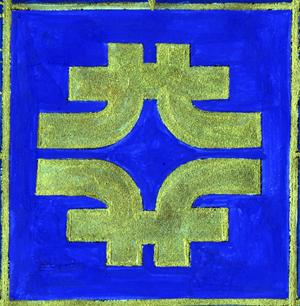
\includegraphics[height=0.50in]{$TEXMFHOME/Figures/Institutions/FNAL.jpg}

\includegraphics[height=0.50in]{$TEXMFHOME/Figures/Institutions/FortLewis.jpg}

\includegraphics[height=0.50in]{$TEXMFHOME/Figures/Institutions/GEUni.jpg}

\includegraphics[height=0.50in]{$TEXMFHOME/Figures/Institutions/Hawaii.jpg}

\includegraphics[height=0.50in]{$TEXMFHOME/Figures/Institutions/Houston.jpg}

\includegraphics[height=0.50in]{$TEXMFHOME/Figures/Institutions/ifusp.png}
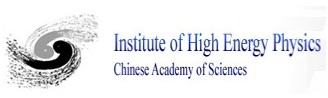
\includegraphics[height=0.50in]{$TEXMFHOME/Figures/Institutions/IHEP.jpg}

\includegraphics[height=0.50in]{$TEXMFHOME/Figures/Institutions/INFN.jpg}

\includegraphics[height=0.50in]{$TEXMFHOME/Figures/Institutions/INPO.jpg}
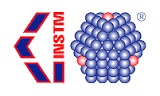
\includegraphics[height=0.50in]{$TEXMFHOME/Figures/Institutions/INSTM.jpg}
%
\includegraphics[height=0.50in]{$TEXMFHOME/Figures/Institutions/IPHC.jpg}

\includegraphics[height=0.50in]{$TEXMFHOME/Figures/Institutions/JINR.jpg}

\includegraphics[height=0.50in]{$TEXMFHOME/Figures/Institutions/Krakow.jpg}

\includegraphics[height=0.50in]{$TEXMFHOME/Figures/Institutions/Kurchatov.jpg}

\includegraphics[height=0.50in]{$TEXMFHOME/Figures/Institutions/Laurentian.jpg}

\includegraphics[height=0.50in]{$TEXMFHOME/Figures/Institutions/LNFINFN.jpg}

\includegraphics[height=0.50in]{$TEXMFHOME/Figures/Institutions/LPNHE.jpg}

\includegraphics[height=0.50in]{$TEXMFHOME/Figures/Institutions/logo_Lodz.jpg}

\includegraphics[height=0.50in]{$TEXMFHOME/Figures/Institutions/Manchester.jpg}

\includegraphics[height=0.50in]{$TEXMFHOME/Figures/Institutions/MEPhI.jpg}

\includegraphics[height=0.50in]{$TEXMFHOME/Figures/Institutions/MIPoli.jpg}

\includegraphics[height=0.50in]{$TEXMFHOME/Figures/Institutions/MIUni.jpg}

\includegraphics[height=0.50in]{$TEXMFHOME/Figures/Institutions/MSU.jpg}

\includegraphics[height=0.50in]{$TEXMFHOME/Figures/Institutions/NAUni.jpg}

\includegraphics[height=0.50in]{$TEXMFHOME/Figures/Institutions/NSU.jpg}

\includegraphics[height=0.50in]{$TEXMFHOME/Figures/Institutions/Petersburg.jpg}

\includegraphics[height=0.50in]{$TEXMFHOME/Figures/Institutions/PGUni.jpg}

\includegraphics[height=0.50in]{$TEXMFHOME/Figures/Institutions/PIUni.jpg}

\includegraphics[height=0.50in]{$TEXMFHOME/Figures/Institutions/PNNL.jpg}

\includegraphics[height=0.50in]{$TEXMFHOME/Figures/Institutions/Princeton.jpg}

\includegraphics[height=0.50in]{$TEXMFHOME/Figures/Institutions/Queens.jpg}
\includegraphics[height=0.50in]{$TEXMFHOME/Figures/Institutions/RHUL.jpg}
\includegraphics[height=0.50in]{$TEXMFHOME/Figures/Institutions/RMUnoUni.jpg}
\includegraphics[height=0.50in]{$TEXMFHOME/Figures/Institutions/RMTreUni.jpg}
\includegraphics[height=0.50in]{$TEXMFHOME/Figures/Institutions/SAUni.jpg}
\includegraphics[height=0.50in]{$TEXMFHOME/Figures/Institutions/SNOLab.jpg}
\includegraphics[height=0.50in]{$TEXMFHOME/Figures/Institutions/Sussex.jpg}
\includegraphics[height=0.50in]{$TEXMFHOME/Figures/Institutions/SSUni.jpg}
\includegraphics[height=0.50in]{$TEXMFHOME/Figures/Institutions/Temple.jpg}
\includegraphics[height=0.50in]{$TEXMFHOME/Figures/Institutions/TNFBK.jpg}
\includegraphics[height=0.50in]{$TEXMFHOME/Figures/Institutions/TNTIFPA.jpg}
\includegraphics[height=0.50in]{$TEXMFHOME/Figures/Institutions/TNUni.jpg}
\includegraphics[height=0.50in]{$TEXMFHOME/Figures/Institutions/TOPoli.jpg}
\includegraphics[height=0.50in]{$TEXMFHOME/Figures/Institutions/TOUni.jpg}
\includegraphics[height=0.50in]{$TEXMFHOME/Figures/Institutions/TRIUMF.jpg}
\includegraphics[height=0.50in]{$TEXMFHOME/Figures/Institutions/TUM.jpg}
\includegraphics[height=0.50in]{$TEXMFHOME/Figures/Institutions/UAM.jpg}
\includegraphics[height=0.50in]{$TEXMFHOME/Figures/Institutions/UCDavis.jpg}
\includegraphics[height=0.50in]{$TEXMFHOME/Figures/Institutions/UCLA.jpg}
\includegraphics[height=0.50in]{$TEXMFHOME/Figures/Institutions/UMass.jpg}
\includegraphics[height=0.50in]{$TEXMFHOME/Figures/Institutions/UOC.jpg}
\includegraphics[height=0.50in]{$TEXMFHOME/Figures/Institutions/USP.jpg}
\includegraphics[height=0.50in]{$TEXMFHOME/Figures/Institutions/logoUZ.png}
\includegraphics[height=0.50in]{$TEXMFHOME/Figures/Institutions/VTech.jpg}
\end{center}
%
%---
\clearpage
\newpage
\newpagecolor{white}
%---
\title{\DSk\ Intermediate Design Report}
\author{C.~E.~Aalseth}\affiliation{\PNNLaddress}
\author{S.~Abdelhakim}\affiliation{\IPNO}
\author{F.~Acerbi}\affiliation{\TNFBK}\affiliation{\TNTIFPA}
\author{P.~Agnes}\affiliation{\Houston}
\author{I.~F.~M.~Albuquerque}\affiliation{\USP}
\author{T.~Alexander}\affiliation{\PNNLaddress}
\author{A.~Alici}\affiliation{\BOUniPHY}\affiliation{\BOINFN}
\author{A.~K.~Alton}\affiliation{\Augustana}
\author{P.~Amaudruz}\affiliation{\TRIUMFaddress}
\author{F.~Ameli}\affiliation{\RMUnoINFN}
\author{P.~Antonioli}\affiliation{\BOINFN}
\author{S.~Arcelli}\affiliation{\BOUniPHY}\affiliation{\BOINFN}
\author{R.~Ardito}\affiliation{\MIPoliICA}\affiliation{\MIINFN}
\author{I.~J.~Arnquist}\affiliation{\PNNLaddress}
\author{P.~Arpaia}\affiliation{\NAUniEEIT}\affiliation{\NAINFN}
\author{D.~M.~Asner}\affiliation{\BNLaddress}
\author{A.~Asunskis}\affiliation{\BHSU}
\author{M.~Ave}\affiliation{\USP}
\author{H.~O.~Back}\affiliation{\PNNLaddress}
\author{A.~Barrado~Olmedo}\affiliation{\CIEMAT}
\author{G.~Batignani}\affiliation{\PIINFN}\affiliation{\PIUniPHY}
\author{M.~G.~Bisogni}\affiliation{\PIINFN}\affiliation{\PIUniPHY}
\author{V.~Bocci}\affiliation{\RMUnoINFN}
\author{A.~Bondar}\affiliation{\BINP}\affiliation{\NSU}
\author{G.~Bonfini}\affiliation{\AQLNGS}
\author{W.~Bonivento}\affiliation{\CAINFN}
\author{B.~Bottino}\affiliation{\GEUni}\affiliation{\GEINFN}
\author{M.~G.~Boulay}\affiliation{\Carleton}
\author{R.~Bunker}\affiliation{\PNNLaddress}
\author{S.~Bussino}\affiliation{\RMTreINFN}\affiliation{\RMTreUni}
\author{A.~Buzulutskov}\affiliation{\BINP}\affiliation{\NSU}
\author{M.~Cadeddu}\affiliation{\CAUniPHY}\affiliation{\CAINFN}
\author{M.~Cadoni}\affiliation{\CAUniPHY}\affiliation{\CAINFN}
\author{A.~Caminata}\affiliation{\GEINFN}
\author{N.~Canci}\affiliation{\Houston}\affiliation{\AQLNGS}
\author{A.~Candela}\affiliation{\AQLNGS}
\author{C.~Cantini}\affiliation{\ETHZ}
\author{M.~Caravati}\affiliation{\CAINFN}
\author{M.~Cariello}\affiliation{\GEINFN}
\author{M.~Carpinelli}\affiliation{\SSUniCHP}\affiliation{\CTLNS}
\author{A.~Castellani}\affiliation{\MIPoliICA}\affiliation{\MIINFN}
\author{P.~Castello}\affiliation{\CAUniEEE}\affiliation{\CAINFN}
\author{S.~Catalanotti}\affiliation{\NAUniPHY}\affiliation{\NAINFN}
\author{V.~Cataudella}\affiliation{\NAUniPHY}\affiliation{\NAINFN}
\author{P.~Cavalcante}\affiliation{\VTech}\affiliation{\AQLNGS}
\author{S.~Cavuoti}\affiliation{\NAUniPHY}\affiliation{\NAINFN}
\author{S.~Cebrian}\affiliation{\Zaragoza}
\author{B.~Celano}\affiliation{\NAINFN}
\author{R.~Cereseto}\affiliation{\GEINFN}
\author{W.~Cheng}\affiliation{\TOINFN}\affiliation{\TOPoli}
\author{A.~Chepurnov}\affiliation{\MSU}
\author{C.~Cical\`o}\affiliation{\CAINFN}
\author{L.~Cifarelli}\affiliation{\BOUniPHY}\affiliation{\BOINFN}
\author{M.~Citterio}\affiliation{\MIINFN}
\author{A.~G.~Cocco}\affiliation{\NAINFN}
\author{M.~Colocci}\affiliation{\BOUniPHY}\affiliation{\BOINFN}
\author{L.~Consiglio}\affiliation{\AQGSSI}
\author{F.~Cossio}\affiliation{\TOINFN}\affiliation{\TOPoli}
\author{G.~Covone}\affiliation{\NAUniPHY}\affiliation{\NAINFN}
\author{P.~Crivelli}\affiliation{\ETHZ}
\author{I.~D'Antone}\affiliation{\BOINFN}
\author{M.~D'Incecco}\affiliation{\AQLNGS}
\author{D.~D'Urso}\affiliation{\SSUniCHP}\affiliation{\CTLNS}
\author{M.~D.~Da~Rocha~Rolo}\affiliation{\TOINFN}
\author{M.~Daniel}\affiliation{\CIEMAT}
\author{S.~Davini}\affiliation{\GEINFN}
\author{A.~De~Candia}\affiliation{\NAUniPHY}\affiliation{\NAINFN}
\author{S.~De~Cecco}\affiliation{\RMUnoINFN}\affiliation{\RMUnoUni}
\author{M.~De~Deo}\affiliation{\AQLNGS}
\author{A.~De~Falco}\affiliation{\CAINFN}\affiliation{\CAUniPHY}
\author{G.~De~Filippis}\affiliation{\NAUniPHY}\affiliation{\NAINFN}
\author{D.~De~Gruttola}\affiliation{\SAINFN}
\author{G.~De~Guido}\affiliation{\MIPoliCHE}\affiliation{\MIINFN}
\author{G.~De~Rosa}\affiliation{\NAUniPHY}\affiliation{\NAINFN}
\author{G.~Dellacasa}\affiliation{\TOINFN}
\author{P.~Demontis}\affiliation{\SSUniCHP}\affiliation{\CTLNS}\affiliation{\INSTM}
\author{S.~DePaquale}\affiliation{\SAINFN}
\author{A.~V.~Derbin}\affiliation{\Petersburg}
\author{A.~Devoto}\affiliation{\CAUniPHY}\affiliation{\CAINFN}
\author{F.~Di~Eusanio}\affiliation{\Princeton}\affiliation{\AQLNGS}
\author{G.~Di~Pietro}\affiliation{\AQLNGS}\affiliation{\MIINFN}
\author{P.~Di~Stefano}\affiliation{\Queens}
\author{C.~Dionisi}\affiliation{\RMUnoINFN}\affiliation{\RMUnoUni}
\author{F.~Dordei}\affiliation{\CAINFN}
\author{M.~Downing}\affiliation{\UMass}
\author{F.~Edalatfar}\affiliation{\TRIUMFaddress}
\author{A.~Empl}\affiliation{\Houston}
\author{M.~Fernandez~Diaz}\affiliation{\CIEMAT}
\author{A.~Ferri}\affiliation{\TNFBK}\affiliation{\TNTIFPA}
\author{C.~Filip}\affiliation{\Cluj}
\author{G.~Fiorillo}\affiliation{\NAUniPHY}\affiliation{\NAINFN}
\author{K.~Fomenko}\affiliation{\JINR}
\author{A.~Franceschi}\affiliation{\LNFINFN}
\author{D.~Franco}\affiliation{\APC}
\author{G.~E.~Froudakis}\affiliation{\UOC}
\author{F.~Gabriele}\affiliation{\AQLNGS}
\author{A.~Gabrieli}\affiliation{\SSUniCHP}\affiliation{\CTLNS}
\author{C.~Galbiati}\affiliation{\Princeton}\affiliation{\AQGSSI}
\author{P.~Garcia~Abia}\affiliation{\CIEMAT}
\author{D.~Gasc\'on~Fora}\affiliation{\UB}
\author{A.~Gendotti}\affiliation{\ETHZ}
\author{C.~Ghiano}\affiliation{\AQLNGS}
\author{A.~Ghisi}\affiliation{\MIPoliICA}\affiliation{\MIINFN}
\author{S.~Giagu}\affiliation{\RMUnoINFN}\affiliation{\RMUnoUni}
\author{P.~Giampa}\affiliation{\TRIUMFaddress}
\author{R.~A.~Giampaolo}\affiliation{\TOINFN}
\author{C.~Giganti}\affiliation{\LPNHE}
\author{M.~A.~Giorgi}\affiliation{\PIUniPHY}\affiliation{\PIINFN}
\author{G.~K.~Giovanetti}\affiliation{\Princeton}
\author{M.~L.~Gligan}\affiliation{\Cluj}
\author{A.~Gola}\affiliation{\TNFBK}\affiliation{\TNTIFPA}
\author{O.~Gorchakov}\affiliation{\JINR}
\author{M.~Grab}\affiliation{\Krakow}
\author{R.~Graciani~Diaz}\affiliation{\UB}
\author{F.~Granato}\affiliation{\Temple}
\author{M.~Grassi}\affiliation{\PIINFN}
\author{J.~W.~Grate}\affiliation{\PNNLaddress}
\author{G.~Y.~Grigoriev}\affiliation{\Kurchatov}
\author{A.~Grobov}\affiliation{\Kurchatov}
\author{M.~Gromov}\affiliation{\MSU}
\author{M.~Guan}\affiliation{\IHEPaddress}
\author{M.~B.~B.~Guerra}\affiliation{\BHSU}
\author{M.~Guerzoni}\affiliation{\BOINFN}
\author{M.~Gulino}\affiliation{\ENUniCEE}\affiliation{\CTLNS}
\author{R.~K.~Haaland}\affiliation{\FortLewis}
\author{B.~R.~Hackett}\affiliation{\Hawaii}
\author{A.~Hallin}\affiliation{\Alberta}
\author{B.~Harrop}\affiliation{\Princeton}
\author{E.~W.~Hoppe}\affiliation{\PNNLaddress}
\author{S.~Horikawa}\affiliation{\AQGSSI}\affiliation{\AQLNGS}
\author{B.~Hosseini}\affiliation{\CAINFN}
\author{F.~Hubaut}\affiliation{\CPPM}
\author{P.~Humble}\affiliation{\PNNLaddress}
\author{E.~V.~Hungerford}\affiliation{\Houston}
\author{An.~Ianni}\affiliation{\Princeton}\affiliation{\AQLNGS}
\author{V.~Ippolito}\affiliation{\RMUnoINFN}
\author{C.~Jillings}\affiliation{\Laurentian}\affiliation{\SNOLABaddress}
\author{S.~Jimenez~Cabre}\affiliation{\CIEMAT}
\author{K.~Keeter}\affiliation{\BHSU}
\author{C.~L.~Kendziora}\affiliation{\FNALaddress}
\author{S.~Kim}\affiliation{\Temple}
\author{I.~Kochanek}\affiliation{\AQLNGS}
\author{K.~Kondo}\affiliation{\AQGSSI}
\author{G.~Kopp}\affiliation{\Princeton}
\author{D.~Korablev}\affiliation{\JINR}
\author{G.~Korga}\affiliation{\Houston}\affiliation{\AQLNGS}
\author{A.~Kubankin}\affiliation{\Belgorod}
\author{R.~Kugathasan}\affiliation{\TOINFN}\affiliation{\TOPoli}
\author{M.~Kuss}\affiliation{\PIINFN}
\author{M.~Kuzniak}\affiliation{\Carleton}
\author{M.~La~Commara}\affiliation{\NAUniPHARM}\affiliation{\NAINFN}
\author{M.~Lai}\affiliation{\CAUniPHY}\affiliation{\CAINFN}
\author{S.~Langrock}\affiliation{\Laurentian}\affiliation{\SNOLABaddress}
\author{M.~Lebois}\affiliation{\IPNO}
\author{B.~Lehnert}\affiliation{\Alberta}
\author{X.~Li}\affiliation{\Princeton}
\author{Q.~Liqiang}\affiliation{\IPNO}
\author{M.~Lissia}\affiliation{\CAINFN}
\author{G.~U.~Lodi}\affiliation{\MIPoliCHE}\affiliation{\MIINFN}
\author{G.~Longo}\affiliation{\NAUniPHY}\affiliation{\NAINFN}
\author{R.~Lussana}\affiliation{\MIPoliEIB}\affiliation{\MIINFN}
\author{L.~Luzzi}\affiliation{\MIPoliENE}\affiliation{\MIINFN}
\author{A.~A.~Machado}\affiliation{\Campinas}
\author{I.~N.~Machulin}\affiliation{\Kurchatov}\affiliation{\MEPhI}
\author{A.~Mandarano}\affiliation{\AQGSSI}\affiliation{\AQLNGS}
\author{L.~Mapelli}\affiliation{\Princeton}
\author{M.~Marcante}\affiliation{\TNUni}\affiliation{\TNTIFPA}\affiliation{\TNFBK}
\author{A.~Margotti}\affiliation{\BOINFN}
\author{S.~M.~Mari}\affiliation{\RMTreINFN}\affiliation{\RMTreUni}
\author{M.~Mariani}\affiliation{\MIPoliENE}\affiliation{\MIINFN}
\author{J.~Maricic}\affiliation{\Hawaii}
\author{M.~Marinelli}\affiliation{\GEUni}\affiliation{\GEINFN}
\author{D.~Marras}\affiliation{\CAINFN}
\author{A.~D.~Martinez~Rojas}\affiliation{\TOINFN}\affiliation{\TOPoli}
\author{C.~J.~Martoff}\affiliation{\Temple}
\author{M.~Mascia}\affiliation{\CAUniCHE}\affiliation{\CAINFN}
\author{A.~Masoni}\affiliation{\CAINFN}
\author{A.~Mazzi}\affiliation{\TNFBK}\affiliation{\TNTIFPA}
\author{A.~B.~McDonald}\affiliation{\Queens}
\author{A.~Messina}\affiliation{\RMUnoINFN}\affiliation{\RMUnoUni}
\author{P.~D.~Meyers}\affiliation{\Princeton}
\author{T.~Miletic}\affiliation{\Hawaii}
\author{R.~Milincic}\affiliation{\Hawaii}
\author{A.~Moggi}\affiliation{\PIINFN}
\author{S.~Moioli}\affiliation{\MIPoliCHE}\affiliation{\MIINFN}
\author{J.~Monroe}\affiliation{\RHUL}
\author{M.~Morrocchi}\affiliation{\PIINFN}
\author{T.~Mroz}\affiliation{\Krakow}
\author{W.~Mu}\affiliation{\ETHZ}
\author{V.~N.~Muratova}\affiliation{\Petersburg}
\author{S.~Murphy}\affiliation{\ETHZ}
\author{C.~Muscas}\affiliation{\CAUniEEE}\affiliation{\CAINFN}
\author{P.~Musico}\affiliation{\GEINFN}
\author{R.~Nania}\affiliation{\BOINFN}
\author{T.~Napolitano}\affiliation{\LNFINFN}
\author{A.~Navrer~Agasson}\affiliation{\LPNHE}
\author{M.~Nessi}\affiliation{\CERNaddress}
\author{I.~Nikulin}\affiliation{\Belgorod}
\author{A.~O.~Nozdrina}\affiliation{\Kurchatov}\affiliation{\MEPhI}
\author{N.~N.~Nurakhov}\affiliation{\Kurchatov}
\author{A.~Oleinik}\affiliation{\Belgorod}
\author{V.~Oleynikov}\affiliation{\BINP}\affiliation{\NSU}
\author{M.~Orsini}\affiliation{\AQLNGS}
\author{F.~Ortica}\affiliation{\PGUniCBB}\affiliation{\PGINFN}
\author{L.~Pagani}\affiliation{\UCDavis}
\author{M.~Pallavicini}\affiliation{\GEUni}\affiliation{\GEINFN}
\author{S.~Palmas}\affiliation{\CAUniCHE}\affiliation{\CAINFN}
\author{L.~Pandola}\affiliation{\CTLNS}
\author{E.~Pantic}\affiliation{\UCDavis}
\author{E.~Paoloni}\affiliation{\PIINFN}\affiliation{\PIUniPHY}
\author{G.~Paternoster}\affiliation{\TNFBK}\affiliation{\TNTIFPA}
\author{V.~Pavletcov}\affiliation{\MSU}
\author{F.~Pazzona}\affiliation{\SSUniCHP}\affiliation{\CTLNS}
\author{S.~Peeters}\affiliation{\Sussex}
\author{P.~A.~Pegoraro}\affiliation{\CAUniEEE}\affiliation{\CAINFN}
\author{K.~Pelczar}\affiliation{\AQLNGS}
\author{L.~A.~Pellegrini}\affiliation{\MIPoliCHE}\affiliation{\MIINFN}
\author{N.~Pelliccia}\affiliation{\PGUniCBB}\affiliation{\PGINFN}
\author{F.~Perotti}\affiliation{\MIPoliICA}\affiliation{\MIINFN}
\author{V.~Pesudo}\affiliation{\CIEMAT}
\author{E.~Picciau}\affiliation{\CAUniPHY}\affiliation{\CAINFN}
\author{C.~Piemonte}\affiliation{\TNFBK}\affiliation{\TNTIFPA}
\author{F.~Pietropaolo}\affiliation{\CERNaddress}
\author{A.~Pocar}\affiliation{\UMass}
\author{T.~Pollman}\affiliation{\TUM}
\author{D.~Portaluppi}\affiliation{\MIPoliEIB}\affiliation{\MIINFN}
\author{S.~S.~Poudel}\affiliation{\Houston}
\author{P.~Pralavorio}\affiliation{\CPPM}
\author{D.~Price}\affiliation{\Manchester}
\author{D.~A.~Pugachev}\affiliation{\Kurchatov}
\author{B.~Radics}\affiliation{\ETHZ}
\author{F.~Raffaelli}\affiliation{\PIINFN}
\author{F.~Ragusa}\affiliation{\MIUni}\affiliation{\MIINFN}
\author{M.~Razeti}\affiliation{\CAINFN}
\author{A.~Razeto}\affiliation{\AQLNGS}
\author{V.~Regazzoni}\affiliation{\TNUni}\affiliation{\TNTIFPA}\affiliation{\TNFBK}
\author{C.~Regenfus}\affiliation{\ETHZ}
\author{A.~L.~Renshaw}\affiliation{\Houston}
\author{S.~Rescia}\affiliation{\BNLaddress}
\author{M.~Rescigno}\affiliation{\RMUnoINFN}
\author{F.~Retiere}\affiliation{\TRIUMFaddress}
\author{Q.~Riffard}\affiliation{\APC}
\author{A.~Rivetti}\affiliation{\TOINFN}
\author{A.~Romani}\affiliation{\PGUniCBB}\affiliation{\PGINFN}
\author{L.~Romero}\affiliation{\CIEMAT}
\author{N.~Rossi}\affiliation{\RMUnoINFN}\affiliation{\AQLNGS}
\author{A.~Rubbia}\affiliation{\ETHZ}
\author{D.~Sablone}\affiliation{\Temple}\affiliation{\AQLNGS}
\author{P.~Sala}\affiliation{\CERNaddress}
\author{P.~Salatino}\affiliation{\NAUniCHE}\affiliation{\NAINFN}
\author{O.~Samoylov}\affiliation{\JINR}
\author{E.~S\`anchez~Garc\`ia}\affiliation{\CIEMAT}
\author{S.~Sanfilippo}\affiliation{\RMTreUni}\affiliation{\RMTreINFN}
\author{M.~Sant}\affiliation{\SSUniCHP}\affiliation{\CTLNS}
\author{D.~Santone}\affiliation{\RHUL}
\author{R.~Santorelli}\affiliation{\CIEMAT}
\author{C.~Savarese}\affiliation{\Princeton}
\author{E.~Scapparone}\affiliation{\BOINFN}
\author{B.~Schlitzer}\affiliation{\UCDavis}
\author{G.~Scioli}\affiliation{\BOUniPHY}\affiliation{\BOINFN}
\author{E.~Segreto}\affiliation{\Campinas}
\author{A.~Seifert}\affiliation{\PNNLaddress}
\author{D.~A.~Semenov}\affiliation{\Petersburg}
\author{A.~Shchagin}\affiliation{\Belgorod}
\author{E.~Shemyakina}\affiliation{\BINP}\affiliation{\NSU}
\author{A.~Sheshukov}\affiliation{\JINR}
\author{S.~Siddhanta}\affiliation{\CAINFN}
\author{M.~Simeone}\affiliation{\NAUniCHE}\affiliation{\NAINFN}
\author{P.~N.~Singh}\affiliation{\Houston}
\author{P.~Skensved}\affiliation{\Queens}
\author{M.~D.~Skorokhvatov}\affiliation{\Kurchatov}\affiliation{\MEPhI}
\author{O.~Smirnov}\affiliation{\JINR}
\author{G.~Sobrero}\affiliation{\GEINFN}
\author{A.~Sokolov}\affiliation{\BINP}\affiliation{\NSU}
\author{A.~Sotnikov}\affiliation{\JINR}
\author{R.~Stainforth}\affiliation{\Carleton}
\author{S.~Stracka}\affiliation{\PIINFN}
\author{G.~B.~Suffritti}\affiliation{\SSUniCHP}\affiliation{\CTLNS}\affiliation{\INSTM}
\author{S.~Sulis}\affiliation{\CAUniEEE}\affiliation{\CAINFN}
\author{Y.~Suvorov}\affiliation{\NAUniPHY}\affiliation{\NAINFN}\affiliation{\Kurchatov}
\author{A.M.~Szelc}\affiliation{\Manchester}
\author{R.~Tartaglia}\affiliation{\AQLNGS}
\author{G.~Testera}\affiliation{\GEINFN}
\author{T.~Thorpe}\affiliation{\AQGSSI}\affiliation{\AQLNGS}
\author{A.~Tonazzo}\affiliation{\APC}
\author{A.~Tosi}\affiliation{\MIPoliEIB}\affiliation{\MIINFN}
\author{E.~V.~Unzhakov}\affiliation{\Petersburg}
\author{G.~Usai}\affiliation{\CAINFN}\affiliation{\CAUniPHY}
\author{A.~Vacca}\affiliation{\CAUniCHE}\affiliation{\CAINFN}
\author{E.~V\'azquez-J\'auregui}\affiliation{\UNAM}
\author{M.~Verducci}\affiliation{\RMUnoINFN}\affiliation{\RMUnoUni}
\author{T.~Viant}\affiliation{\ETHZ}
\author{S.~Viel}\affiliation{\Carleton}
\author{F.~Villa}\affiliation{\MIPoliEIB}\affiliation{\MIINFN}
\author{A.~Vishneva}\affiliation{\JINR}
\author{R.~B.~Vogelaar}\affiliation{\VTech}
\author{M.~Wada}\affiliation{\CAINFN}
\author{J.~Wahl}\affiliation{\PNNLaddress}
\author{J.~J.~Walding}\affiliation{\RHUL}
\author{H.~Wang}\affiliation{\UCLA}
\author{Y.~Wang}\affiliation{\UCLA}
\author{S.~Westerdale}\affiliation{\Carleton}
\author{R.~J.~Wheadon}\affiliation{\TOINFN}
\author{R.~Williams}\affiliation{\PNNLaddress}
\author{J.~Wilson}\affiliation{\IPNO}
\author{Marcin~Wojcik}\affiliation{\Krakow}
\author{Mariusz~Wojcik}\affiliation{\Lodz}
\author{S.~Wu}\affiliation{\ETHZ}
\author{X.~Xiao}\affiliation{\UCLA}
\author{C.~Yang}\affiliation{\IHEPaddress}
\author{Z.~Ye}\affiliation{\Houston}
\author{G.~Zuzel}\affiliation{\Krakow}
\pagenumbering{roman}
\maketitle
\clearpage
%---
\onecolumngrid
\setcounter{tocdepth}{2}
\tableofcontents
%---
\makeatletter
\let\toc@pre\relax
\let\toc@post\relax
\makeatother
\clearpage
%---
\listoffigures
\clearpage
%---
\listoftables
\clearpage
%---
\newpage
\pagenumbering{arabic}
\clearpage
%---
\onecolumngrid
%\setcounter{tocdepth}{2}
%\tableofcontents
%---
\newpage
\pagenumbering{arabic}
\clearpage
%---
%---
\section{Executive Summary}
\label{sec:ExecutiveSummary}

{\bf \color{red} La parte iniziale del TDR riassume le motivazioni scientifiche e/o tecnologiche che hanno portato alla proposta per la realizzazione del progetto in questione, un’overview della soluzione proposta e l’evoluzione del progetto nel tempo. Si tratta di un sommario esecutivo dalla lunghezza di 1-2 pagine, che include anche una descrizione sommaria dei contenuti del documento.}

%---
\section{Physics Case}
\label{sec:PhysicsCase}


{\bf\color{red} In questa parte viene riassunto inizialmente il lavoro svolto durante la fase di R\&D del progetto, finanziata nella fase di CDR. Vengono descritti i risultati degli R\&D ma anche i problemi trovati in questa fase, e le soluzioni proposte per risolverli o soluzioni alternative. Vengono anche elencati ulteriori R\&D che si pensa di dover svolgere per finalizzare eventuali scelte tecniche
Inoltre viene descritto il progetto nelle sue generalità e nel suo contesto. Vengono discusse le motivazioni scientifiche che hanno portato alla proposta in questione, con una chiara indicazione degli obiettivi e dei risultati attesi.}


There is strong evidence from astronomical and cosmological observations for the existence of dark matter in our Universe. Weakly Interacting Massive Particles (\WIMPs) are a well-motivated dark matter candidate that may have been produced in the early Universe but are so massive and weakly interacting that they have yet to be observed in a terrestrial experiment. The observation of \WIMPs\ with masses up to about 1 \si{\TeV\per\square\c} is a major objective of the experimental program at the High Luminosity Large Hadron Collider. Future high energy colliders like the FCC-$hh$ (Future Circular Collider) will be able to extend these searches up to the  \SI{10}{\TeV\per\square\c} mass range~\cite{CERN:2017cq}. Direct and indirect dark matter detection techniques allow for a search program complementary to future colliders. For example, the direct detection of dark matter via elastic scattering of galactic \WIMPs\ from a liquid argon target is a demonstrated technique capable of probing masses well above the reach of the LHC.

Liquid argon (\LAr) is a particularly favorable target for the detection of WIMPs thanks to its excellent event discrimination capabilities. Scintillation light initiated by particles recoiling from atomic electrons (\ERs), the primary source of background in a WIMP direct detection experiment, has a time constant of approximately a microsecond. This is in stark contrast to the nanosecond time constant of scintillation light emitted during an expected WIMP-nuclear recoil event (\NR). The \DEAP\ experiment has exploited this effect via pulse shape discrimination (\PSD) to achieve \ER\ background rejection of \DEAPPSDRejection~\cite{Amaudruz:2018gr,Ajaj:2019wi}. Additional event discrimination in an argon-based detector was demonstrated by the \DSf\ (\DSfs) experiment, which uses a two-phase time projection chamber to measure both the prompt argon scintillation light and the ionized electrons resulting from a particle interaction in the detector. This technique provides excellent position resolution and efficient detector fiducialization while maintaining \PSD\ capabilities~\cite{Agnes:2015gu,Agnes:2016fz}.  \DSfs\ has performed a blind analysis of their data and observed no background events over a run period in excess of two years~\cite{Agnes:2018ep}. In addition to sensitivity to WIMPs with masses above \DSkHighMassThreshold, the two-phase \DSfs\ detector has extended its reach to WIMP masses below \DSlLowMassThreshold\ by detecting single ionizaton electrons extracted from the liquid argon volume~\cite{Agnes:2018fg,Agnes:2018ft}.  With careful control of \ER\ background from local radioactivity and a reduction of the \ce{^39Ar} background, a \DSlApproxMassScale\ \LAr\ detector has the potential to reach the ``neutrino floor'' of solar neutrinos in this low-mass parameter space.


Given the potential reach of an argon-based detector, scientists from all of the major groups currently using \LAr\ to search for dark matter, including \ArDM, \DSfs, \DEAP, and \mCLEAN, have joined to form the Global Argon Dark Matter Collaboration (\GADMC) with a goal of building a series of future experiments that maximally exploit the advantages of \LAr\ as a detector target. 


%---
\subsection{\DSk: The High-Mass Search Program}
\label{sec:DSk}


\begin{figure}[t!]
\includegraphics[width=\columnwidth]{Figures/DSk3D.PDF}
\caption[Artist rendering of the \DSks\ detectors]{Artist rendering of the \DSks\ detectors, with many components omitted for clarity of presentation.  The drawing shows the acrylic (\PMMA) sealed \TPC\  filled with \UAr, surrounded by the veto detector consisting of a \ce{Gd}-loaded acrylic Shell (\GdAS) sandwiched between two atmospheric argon (\AAr) active layers (the Inner Active Buffer, \IAB\ and the Outer Active Buffer, \OAB), all contained in the \pDUNE-like cryostat.  The \OAB\ is optically separated from the rest of the  \AAr\ by a copper vessel.  Technical designs of the support structure of the \TPC\ are already available, and intentionally omitted for clarity of presentation of the main elements.}
\label{fig:DSk3D}
\end{figure}


%\begin{figure}[t!]
%\begin{center}
%\includegraphics[width=\textwidth]{Figures/DSk3D.pdf}
%\caption[Drawing of the \DSk\ detector.]{Drawing of the \DSks\ detector: the \PMMA\ \TPC\ filled with \UAr\ surrounded by the veto detector made of a \ce{Gd}-loaded \PMMA\ shell between two \AAr\ active layers, all contained within a membrane cryostat. The outer active argon layer is optically separated from the \AAr\ by a membrane.  For clarity, the mechanical supports holding the veto and \TPC\ are not shown.}
%\label{fig:DSk3D}
%\end{center}
%\end{figure}


%\begin{figure}[t!]
%\begin{center}
%\includegraphics[width=0.8\textwidth]{Figures/TPC-acrylic-vessel-design.pdf}
%\caption[Drawing of the \DSk\ \LArTPC.]{Drawing of the \DSk\ \LArTPC, detailing the \PMMA\ sealed vessel, \TPC\ field cage, and \DSkPdms\ support structure.    For clarity, the mechanical supports holding the \TPC\ and many other engineering details are not shown.}
%\label{fig:DSk3D}
%\end{center}
%\end{figure}

The immediate objective of the \GADMC\ is construction of the \DSks\ two-phase \LAr\ detector, which will operate in Hall-C of the Gran Sasso National Laboratory (\LNGS).  \reffig{DSk3D} shows a 3D schematic of the \DSks\ detector. \DSks\ detector consists of two nested detectors housed within a \pDUNE-style membrane cryostat~\cite{Abi:2017wp,Acciarri:2016wz}.  

The inner detector is a dual-phase argon time projection chamber (\LArTPC) contained within a vessel made from ultra-pure  acrylic (\PMMA) and filled with \UAr.  The central active volume of the TPC is defined by eight vertical reflector panels and the top and bottom windows of the acrylic vessel. Instead of the traditional copper field cage rings and Indium-Tin-Oxide (\ITO) cathode and anode, \DSks\ will use poly(3,4-ethylenedioxythiophene) polystyrene sulfonate (also known as \PEDOT\ and commercialized under the name \Clevios~\cite{HeraeusDeutschlandGmbHandCOKg:2019wt}). All the TPC surfaces in contact with the active argon volume will be coated with  wavelength shifter tetraphenylbutadiene (\TPB) to convert \LAr\ scintillation light to a wavelength detectable by \SiPMs.  \DSkTilesNumber\ \SiPM-based PhotoDetector Modules (\DSkPdm) arrays will view the argon volume through the top and bottom windows of the acrylic vessel. The height of the \TPC\ is \DSkTPCHeight. The total mass of \LAr\ in the active volume is \DSkActiveMass.

The outer veto detector is made of a passive \ce{Gd}-loaded \PMMA\ shell surrounding the inner detector and between between two active \AAr\ layers.  The \ce{Gd}-loaded \PMMA\ shell moderates neutrons emitted from the \LAr\ \TPC\ until they capture on \ce{Gd}, resulting in the emission of multiple \grs.  The \grs\ interact in the \AAr\ layers and cause scintillation light that is detected by photodetectors, thereby providing an efficient veto of radiogenic neutrons that could result in a \NR\ in the TPC.  The \pDUNE-like cryostat will be surrounded by layers of plastic to moderate cosmogenic and radiogenic neutrons from the rocks surrounding Hall~C.


\begin{figure}[t!]
\begin{center}
\includegraphics[width=\textwidth]{./Figures/DSklSensitivitySimplified.pdf}
\caption[Current \DM\ limits and sensitivities for future experiments.]
{\SI{90}{\percent} C.L. exclusion limits showing leading results from direct (continuous lines, Ref.~\cite{Angloher:2012kl,Akerib:2017kg,Cui:2017kg,Aprile:2018ct,Agnes:2018ep,Agnes:2018fg}) and accelerator-based dark matter searches (region above the yellow line \cite{TheATLASCollaboration:2018to}) compared with sensitivities of future germanium-, xenon-, and argon-based direct searches (dashed lines, Ref.~\cite{Nelson:2014wy,Kudryavtsev:2015hy,Aprile:2015wv,Boulay:2017tn,Agnese:2017fn} and this work).  The ``neutrino floor'' curve follows the definition of Ref.~\cite{Billard:2014cx}. The 95\% C.L. limit from the ATLAS Experiment is shown for a benchmark model in which Dirac-fermion WIMPs interact with ordinary matter via a vector mediator with coupling strengths to quarks, leptons and WIMPs of 0.25, 0.01, and 1, respectively~\cite{Abercrombie:2015to}.}
\label{fig:DSklSensitivitySimplified}
\end{center}
\end{figure}

The \DSks\ detector will have ultra-low backgrounds and the ability to measure its backgrounds {\it in situ}, resulting in an expected sensitivity to \WIMP-nucleon cross sections of \DSkSensitivityOneGeVUnit\ (\DSkSensitivityTenGeVUnit) for \WIMPMassOneTev\ (\WIMPMassTenTev) WIMPs following a \DSkRunTimePlannedVerbal\ run.  This projected sensitivity is a factor of~\DSkSensitivityImprovementOneTeV\ better than currently-published results above \WIMPMassOneTev\ and covers a large fraction of the parameter space currently preferred by supersymmetric models.

The sensitivity would further improve to \DSkExtendedSensitivityOneGeVUnit\ (\DSkExtendedSensitivityTenGeVUnit) for \WIMPMassOneTev\ (\WIMPMassTenTev) WIMPs for a \DSkExtendedRunTimePlannedVerbal\ run with a \DSkExtendedExposure\ exposure, see \reffig{DSklSensitivitySimplified}.  During the \DSkExtendedExposure\ exposure, \DSkNuInducedBackgroundExtendedExposureBare\ \NRs\ events are expected from the coherent scattering of atmospheric neutrinos, making \DSks\ the first ever direct dark matter detection experiment to reach this milestone.  The \DSks\ experiment is foreseen to begin operating in 2022 and will either detect \WIMP\ dark matter or exclude a large fraction of favored WIMP parameter space.

\DSks\ is designed to operate with zero backgrounds, meaning that all sources of instrumental background are reduced to \BackgroundFreeRequirement\ over a \DSkExtendedExposure\ exposure.  All background from minimum-ionizing radiation sources will be completely removed thanks to the combined action of \PSD\ of the primary scintillation pulse and comparison of the primary and secondary scintillation (see \refsec{IM-SC-XenonComp} for details on the suppression of background from \PP\ scatters on electrons and Ref.~\cite{Aalseth:2018gq} for that from \ce{^222Rn}, \ce{^220Rn}, and progenies).  \reftab{NeutronBackground} shows the expected radiogenic neutron background contributions of the various detector components following all \TPC\ and veto cuts for the full \DSks\ exposure.  The only remaining background for \WIMP\ searches will be the signal from the coherent scattering of atmospheric neutrinos on argon nuclei, with an expected \DSkNuInducedBackgroundExtendedExposureUnit\ over the \DSkExtendedExposure\ exposure.  \DSks\ will thus be the first experiment in a position to detect this important signal.

This outstanding sensitivity to coherent nuclear recoils will enables \DSks\ to detect a supernova neutrino burst coming from anywhere in the Milky Way Galaxy and, for a majority of the galaxy, clearly identify the neutronization burst. \DSks\ would perform a flavor-blind measurement of the total neutrino flux and average energy, setting an overall normalization that is not affected by neutrino oscillations. When combined with a flavor-specific measurement from a detector like Super-Kamiokande or DUNE, this observation could have sensitivity to the neutrino mass hierarchy. 


%\begin{table*}[t]
%\small
%\begin{tabular}{lccccccc}
%\hline \hline
%\multirow{2}{*}{Material}
%										&Mass			&\ce{^238U}		&\ce{^226Ra}	& $^{232}$Th	&Neutrons		&+\TPC			&+\TPC+veto\\
%         								&[\si{tonne}]	&[\si{\milli\becquerel\per\kg}]
%																		&[\si{\milli\becquerel\per\kg}]
%																						&[\si{\milli\becquerel\per\kg}]
%																										&[\DSkExtendedRunTimePlanned]$^{-1}$
%																														&[\DSkExtendedExposure]$^{-1}$
%																																		&[\DSkExtendedExposure]$^{-1}$\\
%\hline
%\TPC\ Vessel							&\num{2.7}		&\num{1.2E-2}	&\num{10}		& \num{4.1E-3}	&\num{5.7E2}	&\num{0.17}		&\num{1.7E-2}\\
%\TPC\ SiPMs								&\num{0.12}		&-				& -				&-				&\num{5.4E3}	&\num{0.16}		&\num{1.6E-2}\\
%\TPC\ Electronics						&\num{1.0}		&-				& -				&-				&\num{1.2E4}	&\num{0.36}		&\num{3.6E-2}\\
%\TPC\ Mechanics							&\num{1.1}		&\num{3.9}		&\num{3.9}		&\num{1.9}		&\num{9.0E2}	&\num{1.8E-2} 	&\num{2.0E-3}\\
%Veto \SiPMs+elec.						&\num{0.40}		&-				&-				&-				&\num{6.4E3} 	&\num{0.10}		&\num{1.0E-2}\\
%Veto Acrylic							&\num{13}		&\num{1.2E-2}	&\num{10}		&\num{4.1E-3}	&\num{2.6E3}	&\num{4.2E-2} 	&\num{4.0E-3}\\
%Veto Reflectors							&\num{1.0}		&\num{1.2E-2}	&\num{1.0}		&\num{4.1E-3}	&\num{2.0E2}	&\num{2.4E-2} 	&\num{2.0E-3}\\
%Veto Steel								&\num{1.1}		&\num{3.9}		&\num{3.9}		&\num{1.9}		&\num{9.0E2}	&\num{1.4E-2}	&\num{1.0E-3}\\
%\ce{Gd_2(SO_4)_3} $\alpha$'s on self	&\num{0.26}		&\num{7.0}		&\num{7.0}		&\num{0.2}		&\num{1.1E2}	&\num{2.0E-3}   &\num{<1.0E-3}\\
%\ce{Gd_2(SO_4)_3} $\alpha$'s on \PMMA	&\num{0.26}		&\num{7.0}		&\num{7.0}		&\num{0.2}		&\num{3.6E2} 	&\num{6.0E-3}	&\num{1.0E-3}\\
%Copper Cage								&\num{1.0}		&\num{0.30}		&\num{0.30}		&\num{2.0E-2}	&\num{6.0}		&\num{<1.0E-3}	&\num{<1.0E-3}\\
%Cryostat Steel							&\num{250}		&\num{50}		&\num{1.0E3}	&\num{3.9}		&\num{1.0E6}	&-				&\num{<1.0E-3}\\
%Cryostat Insulation 					&\num{40}		&\num{3E3}		&\num{8.0E3}	&\num{3.0E3}	&\num{8.0E7}	&-				&\num{<1.0E-3}\\
%\hline
%{\bf Total}								&				&				&				&				&				&\num[math-rm=\mathbf]{0.9}
%																																		&\num[math-rm=\mathbf]{0.09}\\ 
%\hline
%\end{tabular}
%\caption[Radiogenic neutrons sourced by the detector construction materials and background before and after cuts.]{Radiogenic neutrons sourced by the \LArTPC\ construction materials, veto and cryostat materials, with details of expected contamination levels, background after \TPC\ cuts, and residual background after combined \TPC\ and veto cuts, all relative to the full \DSkExtendedRunTimePlanned\ run time and the full fiducial \DSkExtendedExposure\ exposure.  The number of neutrons source is calculated from the expected contamination levels and material composition.  Note that no specific activity is reported for the \TPC\ \SiPMs\ and associated electronics: in this case the predicted neutron yield is the results of an extremely detailed calculation, accounting for the cumulative contribution of several tens of components, individually assayed.  The same consideration holds for the veto \SiPMs\ and electronics, whose contribution is reported in combination.  For neutrons due to ($\alpha$,n) reactions from $\alpha$'s from impurities in \ce{Gd_2(SO_4)_3}, the contribution is broken down between those due reactions on \ce{Gd} sulfate itself and those due to reactions in the \PMMA\ matrix containing the \ce{Gd} sulfate; the mass fraction of \ce{Gd} in the \GdAS\ \SI{1}{\percent}, for the anticipated \SI{2}{\percent} concentration by mass of \ce{Gd_2(SO_4)_3}.  (For ease of conversion: $\SI{1}{\ppt}(\ce{^238U}) \simeq \SI{1.2e-2}{mBq/kg}$; $\SI{1}{\ppt}(\ce{^232Th}) \simeq$ \SI{4.1e-3}{mBq/kg}.)}
%\label{tab:NeutronBackground}
%\end{table*}

%---
\subsection{\DSl: The Low-Mass Search Program}
\label{sec:DSl}


In parallel to \DSks\ detector, the \GADMC\ will pursue the development of an approximately \DSlApproxMassScale\ detector specifically optimized for the detection of low-mass dark matter, \DSl\ (\DSls).  \DSls\ will achieve a lower energy threshold than \DSks\ by triggering on the electroluminescence signal from ionization electrons, thereby adding sensitivity to WIMP masses below \DSlLowMassThreshold\ at the expense of the \PSD\ power afforded by argon prompt scintillation light.  Without \PSD, contributors to the \ER\ background in \DSls\ must be reduced beyond the requirements of \DSks\ through careful detector design and material selection. While the \DSls\ experiment is outside the scope of this proposal, the implementation of \DSk\ project will have direct impacts on the technological advancements required to enable \DSls\ and the goal of reaching the neutrino floor for WIMP masses between \SI{1}{\GeV\per\c\squared} and \SI{10}{\GeV\per\c\squared}, see \reffig{DSklSensitivitySimplified}.  Among these are the development of low-background \DSkPdms~\cite{DIncecco:2018fx,DIncecco:2018hy} and the construction of the \Aria\ cryogenic distillation column, which will completely remove \ce{^85Kr} and reduce \ce{^39Ar} levels to the level of \SI{1}{\micro\becquerel\per\kg}.  The development of \DSls\ may exploit components of the \DSps\ detector under development at \CERN.  Funding for the development, construction, commissioning, and operation of \DSls\ will be separately requested via alternative funding programs.


%---
\subsection{Argo}
\label{sec:Argo}

The ultimate objective of the GADMC is the construction of the \Argo\ detector, which will have a \GADMCFiducialMass\ fiducial mass and will push the experimental sensitivity to the point at which the coherent scattering of atmospheric neutrinos becomes a limiting background. The excellent \ER\ rejection possible in argon will eliminate backgrounds from solar neutrinos, which will extend the sensitivity of \Argo\ beyond that of technologies with more limited \ER\ discrimination. The throughput  of the \Urania\ plant and \Aria\ facility will enable \ArgoTotalMass\ of \UAr\ to be extracted and purified over a period of about \ArgoExtractionPeriod.  In addition to dark matter detection, such a large detector would also have excellent sensitivity to a neutrino burst associated with a galactic supernova.  If located at \SNOLAB\ or at similar depth, \Argo\ will also have the potential to observe \CNO\ neutrinos for the first time and solve the Solar Metallicity Problem~\cite{Franco:2016ex}.  While the construction of \Argo\ is not within the scope of this proposal, the implementation of  \DSk\ project will pave the way for the development of \Argo\ towards the end of the next decade. 

Combined \DSks, \DSls, and \Argo, will completely cover the spin-independent \WIMP\ hypothesis parameter space down to the neutrino floor for WIMP masses from \SI{1}{\GeV\per\square\c} to several hundreds of \si{\TeV\per\square\c}.

%---
\subsection{Comparison with Xenon-Based Experiments and the ``Neutrino Floor''}
\label{sec:IM-SC-XenonComp}

\begin{figure}
\begin{center}
\includegraphics[width=\textwidth]{./Figures/NobleDiscoveryComp.pdf}
\caption{5$\sigma$ discovery potential of the leading future noble liquid dark matter searches.}
\label{fig:NobleDiscoveryComp}
\end{center}
\end{figure}

Next generation dark matter experiments will be sensitive to several sources of neutrinos via $\nu-e$ elastic scattering and coherent elastic neutrino scattering (\CEnNS) on nuclei (\NR). Atmospheric and diffuse supernovae neutrinos, which due to their high energies can produce \NRs\ in excess of \SI{20}{\keVr}, will be the dominant \CEnNS\ background contributor for WIMP masses above \DSkHighMassThreshold. Solar neutrinos are the main \CEnNS\ background for dark matter masses below \DSlLowMassThreshold. With  argon's ability to discriminate \ER\ from \NR\ to better than a part in \DEAPPSDRejection, \CEnNS\ represents the only irreducible background for a large exposure argon dark matter search. The neutrino background is exacerbated in liquid xenon detectors, which, due to their limited \ER\ rejection power, accept a non-negligible number of $\nu-e$ elastic scatters as signal. 

When calculating the discovery sensitivity of a large dark matter search experiment, one must fully account for the presence of neutrino-induced backgrounds.  We note that the position of the ``neutrino floor'', initially conceived as indicative of the maximum sensitivity attainable by an experiment in the presence of \CEnNS\ background, is critically dependent on the target, experimental technique, statistical analysis, neutrino flux uncertainty and theoretical cross section uncertainty. We therefore include a detailed accounting of the \CEnNS\ and $\nu-e$ backgrounds in the sensitivity and discovery potential curves shown in \reffig{DSklSensitivitySimplified} and \reffig{NobleDiscoveryComp}. We conservatively estimate a \SI{20}{\percent} uncertainty on the neutrino background for high-mass (\DSkHighMassThreshold) searches with \Argo.  This accounts for a \SI{15}{\percent} uncertainty on the atmospheric neutrino flux at mid-latitude locations, such as \SNOLAB\ or \LNGS, based on the latest data-driven models of cosmic primaries~\cite{Evans:2017hu} as well as models of solar cycle, seasonal, geographic, and geomagnetic dependence of the neutrino flux~\cite{Honda:2011ey,Barr:2006ih}.  Additionally, we account for a \SI{5}{\percent} theoretical uncertainty on the Standard Model interaction cross-section, driven by uncertainties on the nuclear form factor and the expected constraints that the COHERENT collaboration will place on non-Standard Model contributions using a \LAr\ target~\cite{Tayloe:2018jn}, which in turn is driven by their current \SI{10}{\percent} uncertainty on neutrino flux~\cite{Akimov:2017bs} and a \SI{6}{\percent} uncertainty on the \LAr\ response as measured by \SCENE~\cite{Cao:2015ks,Alexander:2013ke} and \ARIS~\cite{Agnes:2018cn}.  Planned improvements of COHERENT, including a sharper characterization of the neutrino flux and a measurement with a \LAr\ target, would further reduce the uncertainty on the neutrino background below \SI{10}{\percent}, strongly benefiting the \DSks, and \Argo\ experiments.

Within this framework, we calculate the 5$\sigma$ discovery potential for \DSks\ and \Argo\ and compare it with that of the near-future \LXe\ experiment LZ~\cite{Dobson:2018us}.  As seen from \reffig{NobleDiscoveryComp}, \DSks\ has significantly greater discovery potential than that of LZ.


%---
\subsection{Completed R\&D for \DSks Program}
\label{sec:technologies}

The following technologies are key to the success of \DSk\ project and the long term scientific goals of the \GADMC. Their development will also have potentially wide-reaching effects within the physics community.

{\bf Low-Radioactivity Underground Argon with \Urania~\cite{Aalseth:2018gq}:} 
The \DSfs\ experiment established that \UAr\ is depleted of \ce{^39Ar} by a factor of approximately 1400, a sufficiently low rate to be deployed in a detector the size of \DSks. However, constructing \DSks\ will require that large amounts of \UAr\ be procured in a timely fashion. This will be accomplished by Urania, an argon extraction and purification plant capable of extracting \UraniaUArRate\ of \UAr.  The Urania plant is fully funded by the INFN and will be built by a contracted vendor following specifications established by the Urania Project team. The tender process for the plant's final design, construction, and shipment to the installation site in Cortez, Colorado, is underway and will conclude by the of end of July 2019 with the selection of a contractor.  The preparation of the extraction site, as well as the installation and commissioning of the plant, falls under the responsibility of the U.S. \NSF-supported groups.  The Urania \UAr\ extraction plant is projected to collect approximately \UraniaTotalDSkProduction\ of argon for use in \DSks\ detector by 2022 and could continue to produce underground argon for \Argo\ and other interested particle physics experiments that require \UAr\ to achieve their scientific objectives.  

{\bf Purification and Active Depletion with \Aria~\cite{Aalseth:2018gq}:}
The \Aria\ plant is a \SI{350}{\m} tall cryogenic distillation column that was designed to explore the possibility of chemically separating argon isotopes.  The construction of \Aria\ is fully supported by \INFN\ and Regione Autonoma della Sardegna. 

{\bf SiPM-based Cryogenic Photosensors~\cite{Aalseth:2018gq,DIncecco:2018hy,DIncecco:2018fx}:}
The development of low-background, large-area, cryogenic silicon photomultiplier (SiPM) detectors capable of replacing conventional photomultiplier tubes is critically important for achieving the desired sensitivity of \DSks\ and other large-scale \LAr-based experiments, including DUNE, and LXe-based detectors, such as \nEXO~\cite{Ostrovskiy:2015jl} and NEXT~\cite{Cebrian:2017dy,GomezCadenas:2016cm,Cebrian:2015du}.  The \DSks\ photodetector modules will be assembled at the Nuova Officina Assergi (\NOA), a dedicated cleanroom packaging facility that will have future utility for any experiment needing large volume silicon detector production.

{\bf \pDUNE\ Liquid Argon Cryostat~\cite{Abi:2017wp,Acciarri:2016wz}:}
\DSks\ detector will operate within a membrane cryostat filled with liquefied atmospheric argon, a technology initially developed at \CERN\ for \pDUNE. Eliminating the organic liquid scintillator veto used in \DSfs\ for the \AAr\ veto has several advantages. With the the \DSks\ \LArTPC\ directly immersed in \AAr, the massive stainless steel vacuum cryostat necessary for \DSfs, and its correspondingly large contribution of background events, can be replaced with a transparent, radio-pure \PMMA\ vessel. Photodetector modules can then be mounted outside of the \PMMA\ vessel, reducing their contribution to the background rate and simplifying their assembly strategy. The \pDUNE\ cryostat has the added advantage that it is scalable, making it a technology appropriate for \Argo.

{\bf Sealed \PMMA\ \TPC~\cite{Boulay:2012er,Nantais:2013jp,Amaudruz:2018gr}:}
The \DEAP\ collaboration has extensive experience developing large, radio-pure sealed \PMMA\ vessels. This technology will be used to build the vessel for the \DSks\ \LArTPC, eliminating the need for some of the most problematic radiogenic neutron contributors in \DSfs, most notably the stainless steel cryostat. The \PMMA\ vessel will also reduce the complexity of the \TPC\ assembly.

%---
\subsection{Ongoing R\&D for \DSks Program}
\label{sec:OngoingRandD}

All the major technologies needed for the design and construction are proven and do not necessitate further R\&D by the collaboration as discussed in the preceding paragraph. Some limited developments are only needed in order to finalize the mass production for SiPM and the production of the Gd loaded acrylic panels for the construction of the neutron veto. In both cases the R\&D is actively on-going and will be finalized by 2020. 






%---
\section{Organization}
\label{sec:Organization}

{\bf \color{red} Definire la struttura organizzativa dell’esperimento:
\begin{itemize}
\item Spokesperson, 
\item Technical Coordinator,
\item Local Responsible,
\item Site Manager,
\item Funds Responsible,
\item GLIMO-S\&E.
\end{itemize}
}


\begin{figure*}[htbp!]
\includegraphics[width=\textwidth]{./Figures/ManagementChart.pdf}
\caption[The organization structure of the \GADMC\ and of the \DS\ project]{The organization structure of the \GADMC\ and of the \DS\ project.}
\label{fig:ManagementChart}
\end{figure*}

The organization structure of the \GADMC\ and of the \DS\ project is defined in \reffig{ManagementChart}. The governance of the \GADMC\ is carried out by two distinct branches: the policy-making branch and the executive branch.

The organization structure of the \DS\ project is defined in \reffig{ManagementChart}. The governance is carried out by two distinct branches: the policy-making branch and the executive branch.

Policy-making is done by the {\bf Institutional Board (IB)}. Each institution is represented within the IB by its PI. The IB is guided by an elected {\bf IB Chair} with a renewable \num{2}~year mandate. The IB is responsible for the definition of rules and the governance of the Collaboration, the overall organization of the Collaboration, the appointment of all managers belonging to the policy-making and executive branches; the final approval of major design changes proposed by the executive branch; and the control of financial and human resources.  The current IB Chair is G.~Batignani (Pisa), elected in November~2016 and re-confirmed in November~2018.

Within the policy-making branch there are three committees charged with providing recommendations to the IB and its Chair.  The members of the three committees are appointed by the IB upon proposal of the IB Chair, taking into account the composition of the Collaboration and the need to represent its diverse composition.  These three committees are:

\begin{compactitem}
\item[\bf The Advisory Board,] consisting of the IB Chair and \num{6}~senior IB members nominated by the IB Chair, of which \num{2}~members are from Italian institutions, \num{1}~member is from a US institution, \num{1}~member is from a Canadian institution, and \num{2}~members are from institutions outside the three countries already listed.  This committee is mandated with advising the IB Chair on IB management issues.
\item[\bf The Membership Committee,] consisting of \num{6}~members nominated by the Advisory Board and confirmed by the IB, as well as \num{2} {\it ex officio} Advisory Board members.  This committee addresses requests from new groups wishing to join the Collaboration, helps define the commitments of new groups, and maintains the database and mailing lists of the collaboration.
\end{compactitem}
\smallskip
There are two additional committees within the policy-making branch charged with providing recommendations to the IB on the communication of scientific and technological results.  The members of the two committees are appointed by the IB upon proposal of the IB Chair, taking into account the composition of the Collaboration and the need to represent its diverse composition.  The two committees are:

\begin{compactenum}
\item[\bf The Speakers' Bureau,] consisting of \num{5}~members nominated by the Advisory Board and confirmed by the IB, \num{1} {\it ex officio} Advisory Board member, and the SP and Deputy SP.  This committee appoints speakers at conferences and workshops and approves material that will be presented on behalf of the Collaboration.
\item[\bf The Editorial Board,] consisting of \num{6}~members nominated by the Advisory Board and confirmed by the IB.  This committee approves the start of paper preparation, guides the internal paper review process, and issues final approval of papers before publication.
\end{compactenum}

The executive branch of the \GADMC\ is led by an elected {\bf Spokesperson (SP)}.  The primary responsibility of the SP is to oversee the \DSks\ experiment, oversee any other scientific efforts pursued by the Collaboration, and act as the Collaboration's primary public face.  The SP is assisted by an elected {\bf Deputy SP (dSP)}.  The mandates of the SP and dSP are \num{3}~years, renewable.  C.~Galbiati and G.~Fiorillo were elected as SP and Deputy SP respectively in December 2016.

The \DSk\ project is organized into \num{3} sub-projects: {\bf the \DSks\ detector}, {\bf \Urania}, and {\bf \Aria}. Each of the sub-projects is managed by two {\bf Project Coordinators (PCs)}, {\it i.e.}, a {\bf Project Leader (PL)} and a {\bf Technical Coordinator (TC)}.  The PL manages the overall progress of the sub-project and is responsible for and coordinates the {\bf Level-1 (L1) Work Groups (WGs)} in which the sub-project tasks and objectives are subdivided and organized, ensuring that the design and construction of the sub-project is carried out on schedule, within the cost ceiling, and in a way that meets the performance and reliability requirements determined within the framework of \GADMC\ resource planning.  The PL plans the schedule and budget, sets deadlines, and monitors quality and progress of the sub-project under their oversight.  The TC is responsible for the sub-project construction and the technical integration of all its components. The TC ensures the implementation of engineering standards and procedures, monitors the overall construction of detectors and infrastructure, and is responsible for the sub-project's integration and safety. The \Aria\ sub-project, due to its complex nature, has an additional PC, a {\bf Community Liaison Officer} charged to act as a link with the local authorities in Sardinia.

In addition to the PCs defined above, three {\bf Project Scientists (PSs)} are charged with the scientific oversight of the detector design and construction to ensure that all technical decisions are fully compliant with the requirements of the project and compatible across all sub-systems.

The management of each sub-project is divided between {\bf Level-1 (L1) Managers} and {\bf Level-2 (L2) Managers}, who are responsible for the direction of the {\bf L1} and {\bf L2 WGs} in which the sub-project are organized and structured.

The {\bf Executive Board (EB)}, which is chaired by the SP and includes as members the dSP, the PSs, all PCs, and all L1 Managers, manages the executive branch of the \GADMC.  The IB Chair is an {\it ex officio} member of the EB.  The SP regularly invites senior PIs charged with significant organization and funding responsibilities but without a formal PC role to the EB meetings.

The PSs and the PCs of \DSks\ and \Urania\ report to the EB.  The PCs of \Aria\ report to the {\bf Scientific Responsible (SR) of \Aria}, which is jointly appointed by \INFN\ and the Regione Autonoma della Sardegna.  The SR of \Aria\ is C.~Galbiati, the inventor and founder of the \Aria\ program.  The SR of \Aria\ reports to the EB.

All PCs and PSs are nominated by the SP to the EB, proposed by the EB to the IB, and appointed by the IB.  PCs are required to pledge that \DSks\ will be their top scientific priority and that they will dedicate a dominant fraction of their research time to their effort within the \GADMC.  The EB and by the IB monitor closely the effectiveness of the PCs.

The L1 Managers are proposed by the PCs, confirmed by the EB, and appointed by the IB.  The L1 Managers report to the PCs.  The L2 Managers are proposed by the L1 coordinators in concurrence with the PCs, confirmed by the EB, and appointed by the IB.  The L2 Managers report to the L1 Managers.

The {\bf Technical Board (TB)}, chaired by the SP and with a membership of the dSP, the PSs, all PCs, and all L1 and L2 Managers, is responsible for the execution of the project.  The IB Chair is an {\it ex officio} member of the TB.  All TB meetings and calls are open to the entire Collaboration.  The TB is the forum where all major and minor decisions affecting the project are debated and finalized.  In its decision making process, the TB typically operates by building consensus.  The TB also monitors the execution of the individual sub-projects and discusses matters at the interface between different sub-projects.  All TB meetings are prepared and chaired by the \DSks\ TC.

The \DS\ resource coordination is delegated to a {\bf Resources Coordinator (RC)}, who has responsibility for the administration of the common fund.  The RC is appointed by the IB upon proposal of the EB.
  
The {\bf Resources Review Board (RRB)} is made up of representatives from the funding agencies providing major contributions to the project, the IB Chair, the SP, the dSP, the RC, and the {\bf Country Representatives (CRs)}, who are appointed by the assembly of PIs supported by any given funding agency and is in charge of the relationship with said agency. The RRB responsibilities include the monitoring and management of the financial instruments that constitute the \GADMC\ resources, defining the national and regional contributions to the project, developing the MoU, and approving in-kind contributions.  The {\bf Financial Board (FB)} is composed of the {\bf CRs} and advises the SP on the specific allocation of tasks and funding requests.

A requirement of the \LNGS\ Safety Management System is the appointment of a collaborator as a {\bf Group Leader in Matters of Safety (GLIMOS)}. The GLIMOS has the primary responsibility for health and safety within the Collaboration, providing an interface with \LNGS.  The GLIMOS is appointed by the \LNGS\ Director upon recommendation by the Collaboration.  An additional requirement of the \LNGS\ Environmental Management System is the appointment of a collaborator as contact person for environmental issues or {\bf Referente Ambientale dell'Esperimento (RAE)}.  The RAE acts as the link between the experimental collaboration and \LNGS\ for all matters concerning environmental protection.  The RAE is appointed by the \LNGS\ Director upon recommendation by the Collaboration management

%---
\subsection{Specific Roles and Responsibilities}
\label{sec:Organization-RolesResponsibilities}

\reftab{ManagerialRoles} offers a brief summary of the most significant executive responsibilities within the 3 sub-projects.

\begin{table}[t]
\begin{center}
%\resizebox{\textwidth}{!}{
\begin{tabular}{cccc}
\hline
\hline
\multirow{3}{*}{{\bf Project Scientists}}
						&\multirow{3}{*}{}					&P.~Meyers			&Princeton\\
						&									&W.~Bonivento		&\INFN\ Cagliari\\
						&									&A.~Razeto			&\INFN\ \LNGS\\
\hline
\multirow{2}{*}{{\bf \DSks\ Project Coordinators}}
						&Project Leader						&E. Scapparone		&\INFN\ Bologna\\
						&Technical Coordinator				&An.~Ianni			&Princeton\\
\hline
\multirow{14}{*}{{\bf \DSks\ L1 Managers}}
						&\DSp\ Managers						&G.~Fiorillo		&\INFN\ Napoli\\
						&Technical Integration Manager		&T.~Napolitano 		&\INFN\ LNF\\
						&Materials Manager					&R.~Santorelli		&CIEMAT\\
						&\ArDM\ Manager						&C.~Regenfus		&ETH Z\"urich\\
						&Inner Detector Manager				&H.~Wang			&UCLA\\
						&Deputy Inner Detector Manager		&E.~Pantic			&UC Davis\\	
						&Outer Detector Manager				&G.~Testera 		&\INFN\ Genova\\			
						&Deputy Outer Detector Manager		&J.~Monroe			&RHUL\\	
						&PhotoElectronics Manager			&A.~Razeto			&\INFN\ \LNGS\\
						&Electronics Manager				&M.~Rescigno		&\INFN\ Roma 1\\
						&Calibration Manager				&J.~Maricic			&Hawai'i\\
						&Offline Manager					&D.~Franco			&CNRS/IN2P3\\
						&\ReD\ Manager						&L.~Pandola 		&\INFN\ \LNS\\
						&Outer Cryostat Manager				&M.~Nessi			&\CERN\\
\hline
\multirow{2}{*}{{\bf \Urania\ Project Coordinators}}
						&Project Leader						&M.~Simeone			&\INFN\ Napoli\\
						&Technical Coordinator				&A.~Renshaw 		&University of Houston\\
\hline
\multirow{3}{*}{{\bf \Urania\ L1 Managers}}
						&Plant Manager						&M.~Simeone 		&\INFN\ Napoli\\
						&Site Preparation and Installation	&A.~Renshaw			&Houston\\
						&Extraction							&H.~Back			&\PNNL\\
\hline
\multirow{5}{*}{{\bf \Aria\ Project Coordinators}}
						&Project Leader						&W.~Bonivento		&\INFN\ Cagliari\\
						&Deputy Project Leader				&F.~Gabriele 		&\INFN\ \LNGS\\
						&Technical Coordinator				&R.~Tartaglia 		&\INFN\ \LNGS\\
						&Deputy Technical Coordinator		&M.~Razeti			&\INFN\ Cagliari\\
						&Community Liason Officer			&A.~Devoto			&\INFN\ Cagliari\\
\hline
\multirow{2}{*}{{\bf \Aria\ L1 Managers}}
						&\SeruciOne\ Manager				&F.~Gabriele 		&\INFN\ \LNGS\\
						&\DArT\ Manager						&W.~Bonivento		&\INFN\ Cagliari\\
\hline
\end{tabular}%}
\caption[Managerial roles of the project]{Overview of the most significant managerial roles within the \DS\ sub-projects.}
\label{tab:ManagerialRoles}
\end{center}
\end{table}

%%---
%\subsection{Partnerships}
%% that is capable of collecting a \ArgoExposure\ exposure while eliminating all backgrounds beyond \NR\ events induced by atmospheric and diffuse supernova background neutrinos. These scientists also agreed to form the Global Argon Dark Matter Collaboration (\GADMC), a consortium of institutes active in the development of argon dark matter experiments.  
%
%The Global Argon Dark Matter Collaboration (\GADMC) is composed of scientists from four \LAr\ dark matter projects (\ArDM\ at \LSC, \DSfs\ at LNGS, and \DEAP\ and \mCLEAN\ at \SNOLAB) who have agreed to unify efforts and construct \DSk\ at \LNGS~\cite{Boulay:2017tn}. These same scientists have signed a Letter of Intent signaling their interest in continuing the collaboration beyond \DSks\ to build a \LAr\ detector with a several hundred tonne fiducial mass. The \GADMC\ will oversee the open access of the currently operating \LAr\ dark matter experiments (\DSfs\ and \DEAP) and scientific data to all \GADMC\ institutions, coordinate the construction of \DSks\ at \LNGS, and coordinate the development of a future \LAr\ dark matter detector with a several hundred tonne fiducial mass.
%
%The \GADMC\ collaboration is currently composed of \num{59} institutions and \num{371} scientists from 15 nations: Brazil, Canada, China, France, Germany, Greece, Italy, Mexico, Poland, Romania, Russia, Spain, Switzerland, the United Kingdom, and the United States of America.
%
%\DSks\ was jointly proposed to the US \NSF, the Italian \INFN, and \LNGS, the host laboratory, in December~2015.  The experiment was first reviewed by a joint panel charged by the Italian \INFN\ and the US \NSF.  The joint review was made possible by NSF statute NSF-14-1999 ``Dear Colleague Letter - International Activities within the Physics Division - Potential International Co-Review''~\cite{USNationalScienceFoundation:2014vy} following approval by the US State Department.  Following the first joint review, the experiment was also reviewed by the \INFN\ {\it Commissione Scientifica Nazionale Seconda} (CSN2), the \INFN\ {\it Comitato Tecnico Scientifico} (CTS),  the \LNGS\ Scientific Committee, and the ``Particle Astrophysics -- Experiment'' panel of \NSF.  Following all reviews, the experiment was approved by \INFN\ and \LNGS\ in April~2017 and by \NSF\ in October~2017.  Following a meeting of participating international funding agencies and laboratories held at the Embassy of Canada in Rome in September~2017, the experiment was officially supported by three participating underground laboratories: the host laboratory \LNGS, Laboratorio Subterr\'aneo de Canfranc (\LSC), and \SNOLAB.  Future reviews of the experiment's progress may also involve a coordinated effort by the Directorates of the three laboratories.
%
%\INFN\ has provided most of the capital funds needed to support the \DSks\ project. R\&D and laboratory set-up costs have been covered by INFN CSN2. Additional funding in Italy, including support for the \Urania, \Aria, and \NOA\ facilities, comes from special and regional funds, the Ministero dello Sviluppo Economico (MISE), the Ministero dell'Istruzione, from the Universita e Ricerca (MIUR), the Regione Abruzzo, and the Regione Autonoma della Sardegna.  The Regione Autonoma della Sardegna and INFN instituted a Comitato di Indirizzo to manage the Aria project.  The Regione Autonoma della Sardegna and \INFN\ instituted a {\it Comitato di Indirizzo} to oversee and monitor the \Aria\ project.
%
%Several groups from Canada joined the Collaboration in September~2017. They have secured funding for the large scale extraction of low-radioactivity argon from \CFI\ in Canada and funding for \DEAP\ R\&D from \NSERC.  An internal proposal for capital funds to support \DSks\ activities was submitted to \TRIUMF\ in October~2017 and was approved for funding.  A proposal to the Canadian \CFI\ for additional capital funds will be submitted October 2019.
%
%University groups from Poland, Russia, Spain, and Switzerland are funded to work on \DSks\ by their funding agencies.  University groups from France, Germany, and the UK are currently participating with support from internal resources and are preparing proposals to each of their funding agencies.
%
%Recently, \INFN\ and The Institute of High Energy Physics of the Chinese Academy of Sciences (\IHEP) reached an agreement to produce the acrylic material for both the \TPC\ and the veto detectors in China.  The production will be carried out by DonChamp, Inc. in Changzhou, the same company providing acrylic for the \JUNO\ experiment.  The \IHEP\ group submitted a request for capital funding to the Chinese Ministry of Science to support the acquisition of the \PMMA\ for the the veto detector and the \LArTPC.
%
%The \DSks\ experiment is hosted by \LNGS.  The \LNGS\ Scientific Committee, which meets two times per year, has oversight of the experiment and has assigned two Committee members as reviewers of \DSks.  The reviewers evaluate technical developments, schedule compliance, and collaboration issues, and report their findings to the \LNGS\ Scientific Committee.  The \LNGS\ Scientific Committee regularly requests that the \GADMC\ provide a written report from the collaboration two weeks before its meetings and present technical results during the meetings' open session, and that the Collaboration management be available for discussion in its closed sessions.  The \LNGS\ Scientific Committee issues a report with its findings after each meeting, which details the progress of the Collaboration and offers recommendations.  The \GADMC\ is also requested to release an annual document to \LNGS\ for inclusion in the {\em LNGS Annual Report}.
%
%Within \INFN, the experiment is regularly reviewed by the CSN2, which oversees technical developments and budget, collaboration, and schedule issues.  CSN2 appoints six permanent referees charged with the review and monitoring of \DSks.  CSN2 meets every second month and on average deals with \DSks\ matters in its plenary session twice per year.  
%
%A strong connection between the \DSks\ funding agencies is fostered through ad-hoc meetings between the \INFN\ management and the management of other funding agencies, including the US \NSF, the US \DOE, the Chinese \IHEP, the French \INDPT, and \CERN. In addition, the \DSk\ management has organized six meetings at the Canadian Embassies of Italy, France, Spain, Mexico, and Poland, and at the Italian Consulate in Montreal, Canada.  The six meetings celebrated the Nobel Prize in Physics awarded to Prof. Art McDonald, who is a founding member of the \GADMC\ and an active participant in \DSks, and took the opportunity to present to a broad audience, which included agency officials and government representatives, the short- and long-term plans of the \GADMC.
%
%
%%---
%\subsection{External Organization and Communication}
%
%The Spokesperson is responsible for external communications.  Relationships with the funding agencies are maintained by the Country Representatives and by the Spokesperson.
%
%
%%---
%\subsection{Institutional Responsibilities}
%
%The assignment of tasks and responsibilities to the various collaborating institutions is captured in a Primavera P6-based resource-loaded work breakdown structure (WBS) managed by the \DSks\ TC and by the project controls team. The WBS is presented in schematic form in \reffig{WBS} and a summary of the institutional participation by task is summarized in \reftab{InstitutionalResponsibilities}.
%
%\begin{table}[t]
%\begin{center}
%\begin{tabular}{lc}
%\hline
%\hline
%\multirow{1}{*}{{\bf Outer cryostat}} 				&\INFN\ (L), \CERN,	UCLA, Princeton\\
%\hline
%\multirow{1}{*}{{\bf Inner detector}} 				&UCLA (L), \FNAL, UMass, \INFN, Alberta, Carleton, Queens, Houston, UC Davis\\
%\hline
%\multirow{1}{*}{{\bf Photoelectronics}} 			&\INFN\ (L), \GSSI, UMass, Princeton\\ 
%\hline
%\multirow{1}{*}{{\bf Outer detector}}				&Genova (L), \LNGS, AstroCeNT, Virginia Tech, Royal Holloway, \IHEP\\
%\hline
%\multirow{1}{*}{{\bf Calibration}}					&Hawai'i (L), Temple, Princeton, BNRU/RSU, Virginia Tech, Krakow, \LNGS, \LNF\\
%\hline
%\multirow{1}{*}{{\bf Electronics}}					&\INFN\ (L), \CERN, \TRIUMF\\
%\hline
%\multirow{1}{*}{{\bf Online\&Offline SW}} 			&APC Paris (L), \INFN, LPNHE, Paris\\ 		
%\hline
%\multirow{1}{*}{{\bf Material screening}} 			&CIEMAT (L), \SNOLAB, Krakow, \INFN, \LSC, LNL, Zaragoza\\
%\hline
%\multirow{1}{*}{{\bf \ReD}}	 						&\INFN\ (L), APC, LNS, USP\\
%\hline
%\multirow{1}{*}{{\bf \DSps}}						&\INFN\ (L),  most \GADMC\ institutions\\
%\hline
%\multirow{1}{*}{{\bf \Urania }} 					&\INFN\ (L), Houston (L), UMass, \PNNL, Carleton\\											
%\hline
%\multirow{1}{*}{{\bf \Aria }} 						&\INFN\ (L), Princeton, \FNAL, \CERN\\	
%\hline
%\multirow{1}{*}{{\bf \DArT }} 						&\LSC\ (L), ETHZ, CIEMAT, APC, Carleton, Zaragoza\\		
%\hline
%\end{tabular}%}
%\caption[Breakdown of institutional responsibilities]{Breakdown of institutional responsibilities. Lead institutions are marked with (L).}
%\label{tab:InstitutionalResponsibilities}
%\end{center}
%\end{table}
%
%%---
%\subsection{Partnerships}
%% that is capable of collecting a \ArgoExposure\ exposure while eliminating all backgrounds beyond \NR\ events induced by atmospheric and diffuse supernova background neutrinos. These scientists also agreed to form the Global Argon Dark Matter Collaboration (\GADMC), a consortium of institutes active in the development of argon dark matter experiments.  
%
%The Global Argon Dark Matter Collaboration (\GADMC) is composed of scientists from four \LAr\ dark matter projects (\ArDM\ at \LSC, \DSfs\ at LNGS, and \DEAP\ and \mCLEAN\ at \SNOLAB) who have agreed to unify efforts and construct \DSk\ at \LNGS~\cite{Boulay:2017tn}. These same scientists have signed a Letter of Intent signaling their interest in continuing the collaboration beyond \DSks\ to build a \LAr\ detector with a several hundred tonne fiducial mass. The \GADMC\ will oversee the open access of the currently operating \LAr\ dark matter experiments (\DSfs\ and \DEAP) and scientific data to all \GADMC\ institutions, coordinate the construction of \DSks\ at \LNGS, and coordinate the development of a future \LAr\ dark matter detector with a several hundred tonne fiducial mass.
%
%The \GADMC\ collaboration is currently composed of \num{59} institutions and \num{371} scientists from 15 nations: Brazil, Canada, China, France, Germany, Greece, Italy, Mexico, Poland, Romania, Russia, Spain, Switzerland, the United Kingdom, and the United States of America.
%
%\DSks\ was jointly proposed to the US \NSF, the Italian \INFN, and \LNGS, the host laboratory, in December~2015.  The experiment was first reviewed by a joint panel charged by the Italian \INFN\ and the US \NSF.  The joint review was made possible by NSF statute NSF-14-1999 ``Dear Colleague Letter - International Activities within the Physics Division - Potential International Co-Review''~\cite{USNationalScienceFoundation:2014vy} following approval by the US State Department.  Following the first joint review, the experiment was also reviewed by the \INFN\ {\it Commissione Scientifica Nazionale Seconda} (CSN2), the \INFN\ {\it Comitato Tecnico Scientifico} (CTS),  the \LNGS\ Scientific Committee, and the ``Particle Astrophysics -- Experiment'' panel of \NSF.  Following all reviews, the experiment was approved by \INFN\ and \LNGS\ in April~2017 and by \NSF\ in October~2017.  Following a meeting of participating international funding agencies and laboratories held at the Embassy of Canada in Rome in September~2017, the experiment was officially supported by three participating underground laboratories: the host laboratory \LNGS, Laboratorio Subterr\'aneo de Canfranc (\LSC), and \SNOLAB.  Future reviews of the experiment's progress may also involve a coordinated effort by the Directorates of the three laboratories.
%
%\INFN\ has provided most of the capital funds needed to support the \DSks\ project. R\&D and laboratory set-up costs have been covered by INFN CSN2. Additional funding in Italy, including support for the \Urania, \Aria, and \NOA\ facilities, comes from special and regional funds, the Ministero dello Sviluppo Economico (MISE), the Ministero dell'Istruzione, from the Universita e Ricerca (MIUR), the Regione Abruzzo, and the Regione Autonoma della Sardegna.  The Regione Autonoma della Sardegna and INFN instituted a Comitato di Indirizzo to manage the Aria project.  The Regione Autonoma della Sardegna and \INFN\ instituted a {\it Comitato di Indirizzo} to oversee and monitor the \Aria\ project.
%
%Several groups from Canada joined the Collaboration in September~2017. They have secured funding for the large scale extraction of low-radioactivity argon from \CFI\ in Canada and funding for \DEAP\ R\&D from \NSERC.  An internal proposal for capital funds to support \DSks\ activities was submitted to \TRIUMF\ in October~2017 and was approved for funding.  A proposal to the Canadian \CFI\ for additional capital funds will be submitted October 2019.
%
%University groups from Poland, Russia, Spain, and Switzerland are funded to work on \DSks\ by their funding agencies.  University groups from France, Germany, and the UK are currently participating with support from internal resources and are preparing proposals to each of their funding agencies.
%
%Recently, \INFN\ and The Institute of High Energy Physics of the Chinese Academy of Sciences (\IHEP) reached an agreement to produce the acrylic material for both the \TPC\ and the veto detectors in China.  The production will be carried out by DonChamp, Inc. in Changzhou, the same company providing acrylic for the \JUNO\ experiment.  The \IHEP\ group submitted a request for capital funding to the Chinese Ministry of Science to support the acquisition of the \PMMA\ for the the veto detector and the \LArTPC.
%
%The \DSks\ experiment is hosted by \LNGS.  The \LNGS\ Scientific Committee, which meets two times per year, has oversight of the experiment and has assigned two Committee members as reviewers of \DSks.  The reviewers evaluate technical developments, schedule compliance, and collaboration issues, and report their findings to the \LNGS\ Scientific Committee.  The \LNGS\ Scientific Committee regularly requests that the \GADMC\ provide a written report from the collaboration two weeks before its meetings and present technical results during the meetings' open session, and that the Collaboration management be available for discussion in its closed sessions.  The \LNGS\ Scientific Committee issues a report with its findings after each meeting, which details the progress of the Collaboration and offers recommendations.  The \GADMC\ is also requested to release an annual document to \LNGS\ for inclusion in the {\em LNGS Annual Report}.
%
%Within \INFN, the experiment is regularly reviewed by the CSN2, which oversees technical developments and budget, collaboration, and schedule issues.  CSN2 appoints six permanent referees charged with the review and monitoring of \DSks.  CSN2 meets every second month and on average deals with \DSks\ matters in its plenary session twice per year.  
%
%A strong connection between the \DSks\ funding agencies is fostered through ad-hoc meetings between the \INFN\ management and the management of other funding agencies, including the US \NSF, the US \DOE, the Chinese \IHEP, the French \INDPT, and \CERN. In addition, the \DSk\ management has organized six meetings at the Canadian Embassies of Italy, France, Spain, Mexico, and Poland, and at the Italian Consulate in Montreal, Canada.  The six meetings celebrated the Nobel Prize in Physics awarded to Prof. Art McDonald, who is a founding member of the \GADMC\ and an active participant in \DSks, and took the opportunity to present to a broad audience, which included agency officials and government representatives, the short- and long-term plans of the \GADMC.
%
%
%%---
%\subsection{External Organization and Communication}
%
%The Spokesperson is responsible for external communications.  Relationships with the funding agencies are maintained by the Country Representatives and by the Spokesperson.
%
%
%%---
%\subsection{Institutional Responsibilities}
%
%The assignment of tasks and responsibilities to the various collaborating institutions is captured in a Primavera P6-based resource-loaded work breakdown structure (WBS) managed by the \DSks\ TC and by the project controls team. The WBS is presented in schematic form in \reffig{WBS} and a summary of the institutional participation by task is summarized in \reftab{InstitutionalResponsibilities}.
%
%\begin{table}[t]
%\begin{center}
%\begin{tabular}{lc}
%\hline
%\hline
%\multirow{1}{*}{{\bf Outer cryostat}} 				&\INFN\ (L), \CERN,	UCLA, Princeton\\
%\hline
%\multirow{1}{*}{{\bf Inner detector}} 				&UCLA (L), \FNAL, UMass, \INFN, Alberta, Carleton, Queens, Houston, UC Davis\\
%\hline
%\multirow{1}{*}{{\bf Photoelectronics}} 			&\INFN\ (L), \GSSI, UMass, Princeton\\ 
%\hline
%\multirow{1}{*}{{\bf Outer detector}}				&Genova (L), \LNGS, AstroCeNT, Virginia Tech, Royal Holloway, \IHEP\\
%\hline
%\multirow{1}{*}{{\bf Calibration}}					&Hawai'i (L), Temple, Princeton, BNRU/RSU, Virginia Tech, Krakow, \LNGS, \LNF\\
%\hline
%\multirow{1}{*}{{\bf Electronics}}					&\INFN\ (L), \CERN, \TRIUMF\\
%\hline
%\multirow{1}{*}{{\bf Online\&Offline SW}} 			&APC Paris (L), \INFN, LPNHE, Paris\\ 		
%\hline
%\multirow{1}{*}{{\bf Material screening}} 			&CIEMAT (L), \SNOLAB, Krakow, \INFN, \LSC, LNL, Zaragoza\\
%\hline
%\multirow{1}{*}{{\bf \ReD}}	 						&\INFN\ (L), APC, LNS, USP\\
%\hline
%\multirow{1}{*}{{\bf \DSps}}						&\INFN\ (L),  most \GADMC\ institutions\\
%\hline
%\multirow{1}{*}{{\bf \Urania }} 					&\INFN\ (L), Houston (L), UMass, \PNNL, Carleton\\											
%\hline
%\multirow{1}{*}{{\bf \Aria }} 						&\INFN\ (L), Princeton, \FNAL, \CERN\\	
%\hline
%\multirow{1}{*}{{\bf \DArT }} 						&\LSC\ (L), ETHZ, CIEMAT, APC, Carleton, Zaragoza\\		
%\hline
%\end{tabular}%}
%\caption[Breakdown of institutional responsibilities]{Breakdown of institutional responsibilities. Lead institutions are marked with (L).}
%\label{tab:InstitutionalResponsibilities}
%\end{center}
%\end{table}
%
%%The outer cryostat task is managed by \CERN\ and \INFN\ and has active participation from UCLA (cryogenic system) and Princeton. 
%
%%The inner detector task is led by UCLA (overall design and cryogenic system) with  contributions from \FNAL\ (cryogenics); Roma1 (test facility); Alberta, Carleton and Queens (machining and assembly of the acrylic parts, TPB coating); Napoli (intergration), Houston (extraction grid); and UC Davis (HV system, field and reflector cage). 
%
%%The photoelectronics task is led by \INFN\ with contributions from Bologna (overall coordination, motherboards, \NOA\ coordination, optical link), \GSSI\ and \LNGS\ (overall system design, front end electronics and tests, optical link), Cagliari (optical link), Pisa (PDMs), Genova and  Naples (testing), Princeton (\SiPM\ packaging), and Milano (cabling). 
%
%%The DAQ task is led by Roma1 with contributions from TRIUMF (readout boards and software) and \LNGS\ (infrastructure and power supply). 
%
%%The outer detector task is led by Genova with contributions from \LNGS\ (\TPB\ evaporation), AstroCeNT (reflectors), Royal Holloway (simulation), and \IHEP\ (\PMMA\ and \ce{Gd}-loaded \PMMA).
%
%%The calibration task is led by Hawaii with contributions from Temple (deployment of external systems); Princeton, BNRU/RSU, Virginia Tech and Krakow (source procurement); and Princeton, \LNGS, and LNF (on-site installation).
%
%%The online and offline software task is led by APC Paris with important contributions from Roma1 (offline software) and LPNHE Paris.
%
%%The Material screening task is led by CIEMAT with materials screenings performed  at \SNOLAB, Krakow, \LNGS\ and \LSC, with additional contributions from LNL (copper cleaning) and Zaragoza (cosmogenic activation studies). 
%
%%The \ReD\ calibration is experiment is led by \INFN\ with contributions from APC, Napoli, Cagliari, Genova, Roma1, LNGS, LNS, Roma3, and USP.
%
%%The \DSps\ effort is led by  Napoli but is a collaborative effort including most of the \DSk\ institutions.
%
%%\Urania\ is led by Napoli (plant design) and Houston (site preparation and installation), and has very important contributions from BNL and PNNL (extraction), as well as Carleton (storage and shipping). 
%
%%\Aria\ is led by \INFN\ with important contributions from Princeton (design and coordination), Cagliari (overall coordination and contact with local authorities) and has important contributions from \LNGS\ (technical coordination and plant management), Napoli (coordination), \FNAL, and \CERN.
%
%%\DArT\ is led by \LSC\ with contributions from ETHZ, CIEMAT, APC, Carleton, and Zaragoza.
%
%%---
%\subsection{Community Relations and Outreach}
%
%The \GADMC\ outreach group, led by {\it Museo Storico della Fisica e Centro Studi e Ricerche Enrico Fermi}, has started the production of a promotional video that starts with a basic introduction to dark matter and its search, continues with a discussion of the design and implementation of the \DSks\ experiment, and concludes with an overview of the societal benefits of the overall \GADMC\ program.  The promotional video will be used online and during live events, such as conferences, seminars, and presentations devoted to the general public.  It will include 2D and 3D video simulations of the future \DSks\ detector, video footage of key elements and locations of the experiment, video recording from the \Aria\ facility featuring the \SeruciZero\ column and the ongoing preparation for \SeruciOne, and simulations of the \Urania\ facility.  The voiceover will be available in several languages.
%
%The Princeton-Gran Sasso Summer School that was established during the operations of \DSf\ is being reinstated and will focus on high-school and undergraduate students from the Cortez-Durango area in Colorado, USA, the area where the \Urania\ plant will be installed and operated.  The program is expected to benefit the underrepresented Native American population through a partnership established with Fort Lewis College in Durango, CO, USA.  The students selected for the program will be offered a course in physics in Princeton followed by an internship at one of the project facilities or partnering institutions for real-world training in technical STEM related areas.
%
%Additional outreach activities will include the organization of visits to \LNGS\ and to the \Seruci\ site of \Aria\ by secondary school students. Students will be prepared in advance of their visit by one-day masterclasses at their local institutions administered by \GADMC\ researchers, during which they will learn about dark matter and the experimental strategy for its detection.  During their visits, they will participate in interactive tutorials on data analysis and will then perform measurements of the cosmic ray flux at different depths using \SiPM-based cosmic ray telescopes.

%---
\section{Project Overview}
\label{sec:ProjectOverview}

{\bf\color{red}Sulla base del disegno concettuale e dei risultati della fase di ricerca e sviluppo identificati nel paragrafo 2 del CDR si illustra la configurazione finale dell’apparato proposto. Le caratteristiche dell’esperimento, quelle dei sistemi e dei sottosistemi 
principali devono essere descritte e riassunte tramite tavole e schema del PBS (Product Breakdown Structure), un esempio mostrato in figura 1.
Vengono altresì mostrati i requisiti del progetto nella presente configurazione.}


\begin{figure*}[t!]
\includegraphics[width=\textwidth]{./Figures/DSk-Overall.pdf}
\caption[Artist rendering of the \DSks\ experiment in Hall C of \LNGS]{Artist rendering of the \DSks\ experiment in Hall C of \LNGS.}
\label{fig:Overall-Design}
\end{figure*}

Many fundamental design parameters for the \DSk\ (\DSks) experiment are based on the successful experience of the \DS\ Collaboration in constructing, commissioning, and operating the \DSf\ (\DSfs) detector in a background-free mode. The many technical details of \DSf\ can be found in~\cite{Agnes:2015gu,Agnes:2016cp,Agnes:2016fw,Agnes:2016fz,Agnes:2016tx,Agnes:2017ck,Agnes:2017cl,Agnes:2017cz,Agnes:2017ec,Agnes:2018cn,Agnes:2018dt,Agnes:2018ep,Agnes:2018fg,Agnes:2018ft}.  The \DSks\ liquid argon time projection chamber (\LArTPC) will, too, be deployed at \LNGS\ in the underground Hall\,C, at the center of a newly constructed active veto system.  \reffig{Overall-Design} shows the rendering of the future installation of \DSks\ in the underground Hall~C of \LNGS and \reffig{DSk3D} shows an overview of the detailed arrangement of the \LArTPC\ and its anti-coincidence veto detector.  The \DSks\ experiment is designed to operate for a minimum of \DSkExtendedRunTimePlanned\ while maintaining an irreducible background level in the \WIMP\ search region of less than \BackgroundFreeRequirement\ for the total exposure.  To achieve this goal, the design parameters of the \DSks\ experiment have been taken directly from \DSfs, where possible.  Design changes have been made where needed in order to accommodate for the much larger size of \DSks\ and to allow the experimental design to be scalable to a detector at the multi-hundred tonne scale.  In building this preliminary design, issues that have arisen because of design choices or materials selections have been dealt with by limited design modifications, and further optimization will continue as the final development work is completed and a full technical design is made.  

\DSks\ will be built by the Global Argon Dark Matter Collaboration (GADMC) and will consist of two detectors: the inner detector and the veto detector, both hosted in a \pDUNE-like cryostat~\cite{Abi:2017wp,Acciarri:2016wz}.   The inner detector is a \LArTPC\ filled with underground argon (\UAr).  The veto detector is made of a plastic shell, loaded with Gd, surrounding the inner detector, sandwiched between two active atmospheric argon (\AAr) layers.  

%\begin{figure}[t!]
%\includegraphics[width=\columnwidth]{Figures/DSk3D.PDF}
%\caption[Artist rendering of the \DSks\ detectors]{Artist rendering of the \DSks\ detectors, with many components omitted for clarity of presentation.  The drawing shows the acrylic (\PMMA) sealed \TPC\  filled with \UAr, surrounded by the veto detector consisting of a \ce{Gd}-loaded acrylic Shell (\GdAS) sandwiched between two atmospheric argon (\AAr) active layers (the Inner Active Buffer, \IAB\ and the Outer Active Buffer, \OAB), all contained in the \pDUNE-like cryostat.  The \OAB\ is optically separated from the rest of the  \AAr\ by a copper vessel.  Technical designs of the support structure of the \TPC\ are already available, and intentionally omitted for clarity of presentation of the main elements.}
%\label{fig:DSk3D}
%\end{figure}

The decision to abandon an organic liquid scintillator veto and to host \DSks\ within a \pDUNE-like cryostat was originally motivated by the need of minimizing the environmental impact on underground \LNGS\ operations, but carries significant performance advantages.  Indeed, operating the \TPC\ directly in the \pDUNE-like cryostat eliminates the need of a cryostat in the immediate proximity of the \UAr\ target, which would significantly contribute to the residual background.  We therefore adopted a new design, with the \UAr-filled \TPC\  immersed in a bath of liquefied \AAr\ held at the same temperature and pressure.  This then allows for the use of a \TPC\ vessel fabricated from the same ultra-pure poly(methyl methacrylate) (acrylic or \PMMA) developed for the \DEAP\ experiment, and thus eliminating the need for a dedicated cryostat or \UAr\ containment vessel.  The outer walls of the \TPC\ will sit approximately \SI{2}{\m} away from inner wall of the cryostat.  The \pDUNE-like cryostat may be surrounded by layers of plastic for moderation of cosmogenic and radiogenic neutrons from the rocks surrounding the \LNGS\ Hall\,C, this option is being investigated.

While this overview section gives a general outline of the project and introduces the major features of the experiment as they stand in the current preliminary design, the real details are given in the subsequent sections. The development of the \SiPM\ photosensors, the \LArTPC\ and its cryogenics and gas handling system, and the materials screening plan that will ensure the radio purity of the experiment, are detailed in Sec.~\ref{sec:PE}, Sec.~\ref{sec:TPCCryo} and Sec.~\ref{sec:Materials}, respectively.  The plan for the calibration of the experiment is given in Sec.~\ref{sec:Calibration}, the design of the veto detector is presented in Sec.~\ref{sec:Veto}, and the details about the data acquisition system and the plan for offline computing are given in Sec.~\ref{sec:DAQ} and Sec.~\ref{sec:Computing}, respectively.  The two ancillary detectors, ReD and \DSp, are described in Sec.~\ref{sec:Red} and Sec.~\ref{sec:Proto}.  Finally, the design and use of the atmospheric argon cryostat, modeled after the ones deployed for ProtoDUNE, are given in Sec.~\ref{sec:Cryostat}, while the procurement of the underground argon (\UAr) target is detailed in the final section, Sec.~\ref{sec:Argon}.  Note that the following forms a preliminary design for an experiment capable of the stated physics goals, but may change as the technical details evolve in the final engineering stages.  \DSks\ will be built to operate for a minimum of \DSkExtendedRunTimePlanned, providing the best sensitivity to high-mass \WIMP\ dark matter.

Energy deposits in the \LAr\ target result in the production of excited and ionized argon atoms, according to the underlying process for recoiling electrons or nuclei. Excited argon atoms, which can also be produced by recombining ionization charge, lead to an efficient formation of argon excimers decaying via the emission of scintillation light characterized by two decay time constants. Both of the components are combine to yield an instant light signal, called \SOne. Due to the deep UV nature (around \ArWaveLength) of this scintillation light, which is absorbed by most materials, a thin layer of wavelength shifter, tetraphenyl butadiene (TPB), must cover all exposed surfaces to convert the photons to those of optical wavelengths for detection by photosensors. Ionization electrons escaping recombination are drifted to the top of the \LAr\ by an applied electric field, where an electric field stronger than the field applied to drift the electrons, extracts the electrons into the gas pocket above the liquid. Here the strong field accelerates the electrons, enough for them to excite (but not ionize) the argon gas, producing a secondary scintillation signal \STwo, proportional to the ionization charge.  Photosensors placed behind the wavelength shifter-coated windows at the top and bottom of the \TPC, read out both scintillation signals (\SOne\ and \STwo) of each event. \SOne\ is used for energy determination, as well as for pulse shape discrimination (PSD).  The latter is derived from the ratio of the prompt and delayed light fractions. \STwo\ is used for energy and 3D position measurements of the event, the vertical coordinate is measured from the drift time between \SOne\ and \STwo, and the horizontal coordinates from the light pattern resulting in the top photosensors from \STwo. 

The octagonal \LArTPC\ will have a height of \DSkActiveHeight\ and a distance between parallel walls of \DSkActiveDiameter.  It will be instrumented with a new kind of photosensors, arrays of \SiPMs, arranged in assemblies called photodetector modules (\DSkPdms). Each \DSkPdm\ has an area comparable to that of a \SI{3}{\inch} photomultiplier tube (\PMT ), with the \LArTPC\ containing \DSkTilesNumber\ \DSkPdms\ in total.  Substantial effort was put into the development of this technology, since \SiPMs\ promise a higher effective quantum efficiency, higher reliability at \LAr\ temperature, and a much higher radiopurity than \PMTs. All of these properties are crucial for \DSks\ since the PSD, which is the most important mechanism for background discrimination in \LAr, depends critically on the light yield.  Additionally, the large material budget of \PMTs\ is often a limiting factor for neutron- and gamma-induced backgrounds. The \LArTPC\ will be equipped with arrays of \SiPMs, totaling \DSkTilesArea\ in area.

In comparison to \DSfs, where a full digitization and recording of the waveform of each \PMT\ could be achieved, a custom scheme for the sampling of the two-orders-of-magnitude higher channel count of the \DSks\ \SiPM\ \DSkPdms\ has to be developed. Design parameters for the data acquisition (DAQ) system are driven by rates and occupancies, as well as leading edge timing and limited charge information from each channel, while compromising as little as possible on energy resolution and pulse-shape discrimination. %The DAQ system is described in Sec.~\ref{sec:DAQ}.

All components of the detector, especially the inner components, like the \LArTPC, the \SiPM\ arrays, and cables, must be made from materials of the highest radiopurity to keep backgrounds as small as possible.

The veto detector consists of three separate volumes:

\begin{compactitem}
\item An inner volume of active liquid \AAr, called the Inner Argon Buffer (\IAB), surrounding the \TPC;
\item A passive shell of acrylic loaded with Gd, called the \ce{Gd}-loaded Acrylic Shell (\GdAS), of octagonal shape mounted around the \IAB.  The \GdAS\ surrounds the TPC in all directions (lateral, top and bottom, with exceptions due to the signal and utility service holes). 
\item An outer active volume of \AAr, called the Outer Argon Buffer (\OAB).
\end{compactitem}

A copper cage which acts as a Faraday cage provides the optical insulation from the rest of the \AAr\ external to OAB and, at the same time, it realizes the necessary electric shield for reducing external noise from contaminating the detector signals.  The details of the veto design and expected performance are given in Sec.~\ref{sec:Veto}.

In order to demonstrate and test technological developments on a scale relevant to \DSks, the collaboration will build and operate a \DSpApproximateMass\ prototype. The project is called \DSp\ (\DSps) and is described in Sec.~\ref{sec:Proto}. \DSp\ will be at an intermediate scale between \DSfs\ and \DSks, able to test a number of full size components intended for use in \DSks.  The size of \DSps\ was chosen to be able to validate detector and \DSkPdm\ components, including the readout system, both from the mechanical and performance aspects of the experiment. The full size cryogenic system will also be tested in this way, especially the argon condenser, the gas pump, and the heat recovery system. Functionality and stability control, as well as safety issues during power failures, purification flow rates and general controls are meant to be explored. \DSps\ also serves to validate the readiness of the various production lines in the different institutions of the collaboration to ensure quality control and assurance for the production of components for \DSks.


%---
%\subsection{Calibrations}
%\label{sec:Overview-Calibrations}

For the \DSk\ detector to reach its physics goals, a comprehensive plan of calibrations for the \LArTPC\ and Veto detectors is necessary.  The calibration equipment and techniques specific to the \DSks\ experiment are described in detail in Sec.~\ref{sec:Calibration}.  In addition to this, it will be important to also utilize measurements taken with external calibration experiments placed within the line of sight of a neutron beam.  In the \SCENE\ experiment,\cite{Cao:2015ks,Alexander:2013ke} a monochromatic, low energy, pulsed neutron beam at the Notre Dame Institute for Structure and Nuclear Astrophysics was used to study the scintillation light yield from recoiling nuclei in a small \LArTPC, but only down to \SCENERecoilsEnergyMax.  The \ARIS\ experiment was exposed to the highly collimated and quasimonoenergetic LICORNE neutron beam at the Institut de Physique Nucl\'eaire d'Orsay (IPNO) in order to study the scintillation response to nuclear and electronic recoils~\cite{Agnes:2018cn}.

The collaboration is now expanding this external calibration work with a new external calibration experiment, the Recoil Directionality (\ReD ) experiment, described in Sec.~\ref{sec:Red}. The \ReD\ detector is a small \LArTPC\ (similar in size to \SCENE ) equipped with the same \SiPM\ tiles planned for use in \DSks. \ReD\ is designed to select and measure single neutron elastic scatters on argon nuclei, by means of a large acceptance neutron spectrometer, composed of an array of liquid scintillator detectors.  Kinematic requirements of the neutron interactions will allow for the precise detection of nuclear recoils in the \LAr, since the neutron energy, scattering angle, and drift field direction can all be precisely measured with the use of external neutron detectors.

  
\section{Photoelectronics}
\label{sec:PE}

Silicon photomultipliers (\SiPMs) are one of the key enabling technologies for large-scale \LAr-based dark matter experiments.  \SiPMs\ will also play an important role in the next generation of \LAr-based neutrino detectors, such as DUNE~\cite{Acciarri:2016wz}, and liquid xenon based detectors for neutrinoless double beta decay, such as nEXO~\cite{Ostrovskiy:2015jl}.  \SiPMs\ have a number of performance advantages over traditional \PMTs, including higher photon detection efficiency (\PDE) and much better single-photon resolution, all while operating at much lower bias voltage. \SiPMs\ can also be efficiently integrated into tiles that cover large areas and feature better radio-purity than \PMTs.

\begin{figure}[!thbp]
\includegraphics[width=0.49\textwidth]{./Figures/PDM-photo.jpg}
\includegraphics[width=0.49\textwidth]{./Figures/MB-photo_cut.jpg}
\caption[The first \DSkPdm\ and first motherboard resulting from the assembly of \DSkPdms]{{\bf Left:} Single channel PhotoDetector Module (\DSkPdm) consisting of   a \DSkTileAreaStd\ tile of  \DSkTileSiPMsCustomNumber\ \SiPMs\ and a front-end board.  {\bf Right:}  The \DSks\ motherboard assembled with \DSkSQBPdmsNumber\ \DSkPdms.}
\label{fig:PDM+MB}
\end{figure}


%---
\subsection{PhotoDetector Modules (\DSkPdm)}

For \DSks, the photosensing unit will be a ``PhotoDetector Module'' (\DSkPdm), consisting of a large tile of \SiPMs\ covering a total area of \DSkTileAreaStd\ operating as a single detector (see the left panel of Figure~\ref{fig:PDM+MB}).  Besides the tile, each module will also contain a cryogenic preamplifier board that will amplify and shape the signal in the immediate proximity of the sensor.  The output of the cryogenic amplifier will be passed on to a signal transmitter, also integrated into the \DSkPdm, and responsible for transmission of the signal through the cryostat penetration.  Finally, the \DSkPdm\ will also include the mechanical structure required to assemble all components and to efficiently dissipate heat in the \LAr\ target, minimizing the production of bubbles. An intelligent power distribution system is also foreseen, capable of disabling individual \DSkPdms\ in case of failure.

The unique challenge in readout presented by \SiPMs\ is mainly due to their capacitance. At \DSkSiPMCapacitancePerArea, a single \SiPM\ with a \DSkSiPMAreaStd\ surface area passes the \si{\nano\farad} scale for capacitance.  Yet, the experiment foresees a photo-sensing area of \DSkTilesArea.  The readout of a \LAr\ calorimeter faced a similar challenge, with capacitance for the individual cells often passing the \si{\nano\farad} scale~\cite{Willis:1974do}.  Early developments on \LAr\ calorimeter readout~\cite{Radeka:1974ca,Radeka:1988ku,Chase:1993dj,Chase:1997fk} demonstrated that the use of a transimpedance amplifier (\TIA) is preferable to a charge integration amplifier where the noise and rise time are very strongly affected by the large detector capacitance.  With this in mind, the \DS\ Collaboration has developed and optimized a \TIA\ (schematic is shown in the left panel of Figure~\ref{fig:TIA+2s3p}) with performance at \LArNormalTemperature\ in mind~\cite{DIncecco:2018fx}.  The specific goal was to maximize the amplification factor while preserving a stable signal bandwidth and \SNR.

The \SiPMs\ readout scheme strongly affects the PDM performance in terms both of \SNR\ and bandwidth of the signal. A hybrid readout scheme, with parallel-series combination of \SiPMs,  first introduced for the MEG experiment~\cite{Ootani:2013cn,Cattaneo:2016dq}, solves at once these two problems. In this configuration, the output signal of an individual \SiPM\ is reduced by a factor equal to the number of \SiPMs\ put in series, but this disadvantage is offset by the attenuation of the noise gain due to the reduction in the input capacitance. Most importantly, a strong improvement of the bandwidth with respect to the parallel readout scheme is achieved, with six \SiPMs\ easily readout by connecting in parallel three branches of two \SiPMs\ put in series (known as the 2s3p configuration~\cite{DIncecco:2018hy}, see right panel of Figure~\ref{fig:TIA+2s3p}) with a bandwidth comparable to the one achievable with a single \SiPM\ in input. Four such readout quadrants are fit in a single PDM, with their output signals summed at the transmission stage.

\begin{figure}[t!]
\includegraphics[width=0.49\textwidth]{./Figures/tia-schem.pdf}
\includegraphics[width=0.49\textwidth]{./Figures/2s3p-schem.pdf}
\caption[Schematic of the transimpedance amplified and summing circuits]{{\bf Left:}  Schematic diagram of the transimpedance amplifier circuit developed to  readout \SiPMs.  {\bf Right}: Schematic diagram of the 2s3p readout scheme optimized for summing six \SiPM\ signal together.}
\label{fig:TIA+2s3p}
\end{figure}


%---
\subsection{Signal Transmission}

The signal transmission from the \DSkPdms\ to the warm electronics is of primary importance for the experiment. Given the high number of independent channels, cables would introduce a large mass in the cryostat with the inherent problems of radio-purity and heat load. The delivery of the PDM signals to the outside world through optical fibers will solve at once these two problems. For this purpose an optical analog cryogenic transmitter has been developed. The prototype boards of the opto-link system (optical driver and optical receiver board) have been recently produced. The optical receiver board (32 channels) was successfully tested, while the optical driver board (25 channels) is at the moment undergoing testing.

The \DSkPdms\ will be located above the anode and below the cathode, fully covering the top and bottom faces of the \LArTPC\ active volume, to detect both the \SOne\ and \STwo\ signals with high efficiency.  The top and the bottom photon readout assemblies will consist of \DSkTilesHalfNumber\ \DSkPdms\ each.  Multiple \DSkPdms\ are mounted to a single motherboard to form two larger basic mechanical units called the square board (\SQB)  and the triangular board (\TRB),  described in Sec.~\ref{sec:TPC} and shown  in Figure~\ref{fig:3D-TRB-SQB}.  The \SQB\ and \TRB\ have the same edge size of \DSkSQBTRBSize.  The \SQB\ and \TRB\ are then used to form the full readout planes (shown in Figure~\ref{fig:TPC-SiPM_pattern}).  The total number of readout channels (top and bottom) is \DSkTilesNumber.


%---
\subsection{\DSkPdm\ Fabrication and Characterization}

Following the successful construction of the first Photo-Detector Module (PDM) in March 2018, the Photo-Electronics Working Group proceeded to the construction of the first Motherboard, shown in  Figure~\ref{fig:PDM+MB}. The FBK company delivered two SiPM runs: the first one with standard doping SiPMs (cell size \DSkSiPMSPADSizeStd\ and quenching resistor \DSkSiPMSPADQuenchingResistorSingleDoping(\LINNormalTemperature)) and the second one with triple doping SiPMs (cell size \DSkSiPMSPADSizeTripleDoping\ and quenching resistor \DSkSiPMSPADQuenchingResistorTripleDoping(\LINNormalTemperature)). Since the latter SiPM type is considered the best candidate for the \DSks\ experiment, we decided to use the single doping SiPMs for the first Motherboard construction, so that the triple doping type could be mounted later, taking advantage of the experience gained with the mounting of the first Motherboard.

\begin{figure} [t]
\includegraphics[width=\columnwidth]{./Figures/Rq.png}
\caption[Variance of impedance of \SiPMs\ quenching resistors]{Average \SiPM\ quenching resistor value vs. wafer number measured at \SI{20}{\celsius} and \SI{-40}{\celsius}.}
\label{fig:Rq} 
\end{figure} 

This \SiPM\ run was characterized by a reasonable yield at \SI{-40}{\celsius} of about \SI{50}{\percent}.  A detailed inspection of the SiPM quenching resistor ($R_q$) showed good uniformity for most of the wafers, while the first and the second wafers (W1,W2) had a \SI{20}{\percent} larger $R_q$ (see Figure~\ref{fig:Rq}). The optimal working voltage of the \SiPM\ is expected to change as a function of $R_q$, so in the forthcoming mass production by the LFoundry company, where hundreds of \SI{8}{\inch} SiPM wafers are scheduled, this quenching resistor spread is not an issue since the \SiPMs\ with similar $R_q$ can be paired.  In this way, each Motherboard, with \DSkPdms\ biased at the same voltage, will be made of devices with similar $R_q$. Due to the limited \SiPMs\ available in the present production we had to use all of them to make the first Motherboard, and thus all were biased with a common voltage despite the slight difference in $R_q$.  As a consequence, the tiles made with \SiPMs\ belonging to wafers~1 and~2 were fed with an overvoltage lower than the optimal one for some of the \SiPMs, i.e. \SI{5}{\volt}.  It is worth noting that a dedicated facility for the Motherboard production is not available yet, and therfore the use of equipment through outsourcing and  additional man power was therefore required.

The tile and the Front-End Board PCBs were made with an \ArlonFiveFiveNT\ substrate, following the experience gained during the first PDM construction. The electronic components were mounted with outsourced equipment, under the supervision of LNGS personnel. The tile PCBs were tested both at warm and at cryogenic temperatures to verify the correct circuit impedance. After the wafer dicing, the SiPMs were shipped from FBK to Princeton University, where the first Motherboard tiles were bonded by personnel from LNGS, Princeton University and TIFPA. A cryogenic epoxy for the SiPM back-side and a wire-bonding connection for the front-side was used. The 27 tiles, each made of \DSkTileSiPMsCustomNumber\ SiPMs, were then shipped to LNGS, using multipurpose acrylic boxes, designed by the Pisa group. This box allows for safe shipping of the tile, offering an adequate protection of the SiPM wire bonding and, at the same, time allows the tile characterization in liquid nitrogen by permitting the insertion of the Front End Board without removing the tile from the box. The tiles underwent a comprehensive test at LNGS both at warm temperature and in LN, including the reverse I-V curve measurement, the power spectrum and the charge spectra. We found just one tile out of the 27 with two SiPM branches (4 SiPMs) not working properly. Another tile showed a noise level higher than the average. These two tiles were therefore excluded from the list of the tiles selected to populate the first Motherboard.

As an example, the left side of Figure~\ref{fig:I-V-SNR} shows the tile I-V curves taken at \LINNormalTemperature, indicating a homogeneous behavior.  

\begin{figure} [t]
\includegraphics[width=0.49\columnwidth]{./Figures/IV_77K.pdf}
\includegraphics[width=0.49\columnwidth]{./Figures/SNR.pdf}
\caption[\SiPM\ $I$-$V$ curves and \SNR]{{\bf Left:} Reverse I-V curves for the \SiPM\ tiles measured at \LINNormalTemperature.  {\bf Right:} \SNR\ of the \num{27} bonded \SiPM\ tiles.}
\label{fig:I-V-SNR} 
\end{figure} 


The right panel of Figure~\ref{fig:I-V-SNR} shows the signal to noise ratio (\SNR) for the 27 tiles at their optimal voltage.  It is worth noting that all of them have a \SNR\ larger than the minimum \SNR\ of \DSkTileChargeSNRSpecification, required by the \DSk\ experiment specifications. For each tile, the \SNR\ was obtained relying on several different procedures and analysis methods.  The bar length in the figure represents the spread of each measurement, depending on the method used.  The signal-to-noise ratio (\SNR) is defined as the ratio between the gain and the width of the baseline noise peak. The gain is measured by fitting the center values of the amplitude multiple peaks and evaluating the slope of a linear fit. The baseline noise is extracted from the average standard deviation of the waveform in a pre-pulse window, 500 ns long, using 500 samples. For most tiles, the distribution of the standard deviation is not symmetric around the peak.  The most important contribution to the noise baseline is the presence of one or more photoelectrons not stimulated by the laser pulse. These can originate from a SiPM having an excess of dark-rate or more probably by an excess of after-pulsing.

Since the distribution is not symmetric, the estimate of the baseline noise is intrinsically biased and two options are possible, corresponding to the mean value or the most probable value (mode). Consequently the \SNR\ is defined in a confidence interval between $\SNR_{\rm min} = {\rm gain}/{\rm noise}_{\rm mean}$ and $\SNR_{\rm max} = {\rm gain}/{\rm noise}_{\rm mode}$.

Figure~\ref{fig:SNR2} shows the \SNR\ obtained with the common over-voltage of \SI{5}{\volt}. Although a few tiles, as expected, manifest a \SNR\ slightly below \DSkTileChargeSNRSpecification, the \SNR\ is quite good for all tiles used in the assembly of the first Motherboard.


%---
\subsection{Motherboard Assembly}

Before assembling the first Motherboard, a full mock-up made of an aluminum Motherboard structure, an FR4 Motherboard strip PCB, \DSkSQBPdmsNumber\ dummy tiles and FEBs, and the PDM acrylic mechanics was mounted at Bologna. Each PCB had the same dimensions of the final one, while the HV/LV and signal layers were not included in the stack-up. The mounting required just a few hours and the overall procedure was validated, while the mechanics of the different components nicely merged, suggesting just a few minor mechanical improvements. 

After these tests, the tiles were finally shipped to Pisa, while the \DSkPdm\ pillars and the copper Motherboard structure were milled at Bologna using \SI{99.997}{\percent} pure copper sold by the Luvata Company. The first Motherboard was equipped with a PCB strip connecting the \DSkPdms, made of a thin stack-up (\SI{0.5}{\milli\meter}) based on a Pyralux substrate and shipped to Pisa to start the mounting of the \DSkSQBPdmsNumber\ \DSkPdms\ on the Motherboard. 

The \DSkPdms\ were assembled in the Pisa clean room, following the prescriptions used for the first \DSkPdm, assembled in March 2018. The mounting of the \DSkSQBPdmsNumber\ \DSkPdms\ on the Motherboard was finalized in few days.  A picture of the first Motherboard, fully equipped with the first \DSkSQBPdmsNumber\  \DSkPdms\ is shown in the right panel of Figure~\ref{fig:PDM+MB}.

In summary the construction of the first Motherboard required the production, testing, selection and bonding of more than 600 \SiPMs. Although a cryogenic probe and an automatic bonder were not available yet, the Collaboration was able to increase the number of successfully built \DSkPdms\ from 1 to \DSkSQBPdmsNumber, in just \num{6} months. The bonding yield exceeded \SI{95}{\percent} (just 1 tile out of the 27 showed problems with the \SiPM\ bonding strategy), while the satisfactory \DSkPdm\ \SNR\ demonstrated the validity of the full Motherboard construction process.

After the completion of the first motherboard, equipped with \DSkSQBPdmsNumber\ \DSkPdms\ each containing  \DSkTileSiPMsCustomNumber\ single dose SiPM's, the collaboration moved to the construction of a second Motherboard, equipped with triple dose \SiPMs.   At the moment, half of the \DSkPdms\ have already been assembled and mounted in the copper structure. The remaining \DSkPdms\ will be mounted within the summer of~2019.  The FEBs were already successfully tested, while the \SiPM\ tiles are currently undergoing testing in LN. The next step in the photo-electronics schedule is the production of about  \DSkPdmsSecondBatchNumber\ \DSkPdms\ for the \DSps\ detector. These \SiPMs\ will be produced by the LFoundry Company in Avezzano, Italy.  The first run is expected in the summer of~2019. 

\begin{figure}[t!]
\includegraphics[width=0.5\columnwidth]{./Figures/SNR2.PDF}
\caption[\SNR\ of the \SiPMs\ tiles of the first motherboard]{\SNR\ of the \DSkSQBPdmsNumber\ \SiPM\ tiles populating the first motherboard while.  Data were recorded while operating the \SiPM\ tiles at an over-voltage of \SI{5}{\volt}.}
\label{fig:SNR2} 
\end{figure} 


%---
\subsection{Mass Production}

The first engineering run, finalized in September 2018 and tested shortly after, showed the capability of the silicon foundry to implement the FBK technology.  The produced \SiPMs\ showed good performance at both room temperature and in liquid nitrogen. A second LFoundry engineering run, presently ongoing, is devoted to the development of the through silicon vias (TSV). This post-production rework requires some delicate mechanical manipulation of the SiPM wafers.

The \DSks\ \SiPM\ packaging foresees the production of more than \DSkPdmsNumberWithSpares\ \DSkPdms\ in \DSkPdmsContructionTime. This remarkable effort requires a large clean room, relying on cutting edge technology equipment and trained personnel.  The \GADMC\ selected for the \NOA\ \DSks\ \SiPM\ packaging facility a clean room at the {\it Tecnopolo dell'Aquila}, with surface exceeding \DSkPdmsCleanRoomSurface.  The clean room will be soon refurbished to comfortably host the needed equipment and personnel.  This facility will be managed by \GSSI, through an agreement with \INFN\ that will soon be finalized.  Concerning the procurement of the equipment for the \DSks\ \DSkPdms\ mass production, the cryogenic probe tender was just approved by the \INFN\ Executive Board and the flip-chip bonder tender will follow in the weeks to come.
%---
\subsection{Inner Detector and Cryogenics System}
\label{sec:TPCCryo}


%---
\subsubsection{\DSks\ \LArTPC}  
\label{sec:TPC}


The \DSk\ \LArTPC\ is the dark matter detector and the central element of the experiment, with all auxiliary detectors and systems specified and designed in support of it.  The \DSks\ \LArTPC\ will use \DSkCryogenicsCapableLArMass\ of \LAr\ extracted from an underground source as the target material for \WIMP\ detection.   An ultra-pure acrylic vessel is used to contain the \LAr.  Features directly fabricated onto the inner surfaces of the acrylic vessel will form the \TPC\ itself.  These feature are the \TPC\ field cage system, the anode and the cathode and are implemented on the acrylic panels with a commercial conductive polymer coating, called \Clevios.  Use of this coating eliminates the use of metal conductive materials. 

The same pure acrylic material, in the form of \DSkPMMATPCBackPanelThicknessESR\ thick sheets, is used to hold the Enhanced Specular Reflector (\ESR) reflector foils installed to maximize light collection. The \TPC\ is designed such that all the inner surfaces facing the active volume are coated with \TPB, a wavelength shifter, to ensure the complete conversion of the \ArWaveLength\ argon scintillation light to \TPBWaveLength, where the \SiPMs' peak in their PDE.  Two identical photosensor arrays of \DSkTilesHalfNumber\ channels each are placed on top and bottom of the \TPC, but outside of the acrylic vessel. The \TPC\ is mounted inside a neutron veto detector, whose most important component is a \DSkPMMAVetoPanelThickness\ thick, gadolinium loaded, acrylic shell that completely incapsulates the \TPC. This plastic shell defines two \DSkVetoLArThickness\ thick active volumes, respectively named the inner and outer buffer, filled with liquid \AAr. The buffers are further segmented with \ESR, also coated with \TPB. The whole apparatus is placed inside a light and electromagnetic shield barrier, contained in the \pDUNE-like cryostat filled with \AAr.

\begin{table}
\rowcolors{3}{gray!35}{}
\centering
\begin{tabular}{lc}
\hline
\hline
{\bf \DSks\ \TPC\  Dimensions} 		&\\
\hline
\TPC\ Drift Length					&\DSkActiveHeight\\
Octagonal Inscribed Circle Diameter	&\DSkActiveDiameter\\ 
Total \LAr\ Mass 					&\DSkTotalMass\\
Active \LAr\ Mass 					&\DSkActiveMass\\
Fiducial Cut Distance (vertical)	&\DSkVetoFVTPCcutz\\
Fiducial Cut Distance (radial)		&\DSkVetoFVTPCcut\\
Fiducial \LAr\ Mass 				&\DSkFiducialMass\\
\hline
{\bf Nominal \TPC\ Fields and Settings}
									&\cellcolor{white}\\
\hline
Drift Field 						&\DSkDriftField\\
Extraction Field  					&\DSkExtractionField\\
Luminescence Field 					&\DSkElectroLuminescenceField\\
Cathode Voltage 					&\DSkCathodePotential\\
Extraction Grid Voltage		  		&\DSkGridPotential\\
Anode Voltage  						&\DSkAnodePotential\\
Gas Pocket Thickness  				&\DSkGasPocketThickness\\
Grid Wire Spacing  					&\DSkLArOverGridPitch\\
Grid Optical Transparency  			&\DSkGridTrasparency\\
\hline
{\bf \SiPM\ \DSkPdm}				&\cellcolor{white}\\
\hline
Number of \DSkPdm\ on \TPC\ Top		&\DSkTilesHalfNumber\\
Number of \DSkPdm\ on \TPC\ Bottom	&\DSkTilesHalfNumber\\
\DSkPdm\ Effective Area 			&\DSkTileAreaStd\\ 
\hline
\end{tabular}
\caption[\DSks\ \LArTPC\ detector parameters]{\DSks\ \LArTPC\ detector parameters.}
\label{tab:LArTPC-Parameters}
\end{table}

{\bf Sealed \PMMA\ Vessel:} An acrylic (\PMMA) vessel will be used to confine the \UAr\ rather than a metallic vessel, since \PMMA\ is extremely radiopure, resulting in a residual neutron background estimated to be \DSkVetoPMMANeutronResidualBackground\ for the exposure of \DSkExtendedExposure.  As described above, the \TPC\ active volume is confined in all directions by the sealed \PMMA\ vessel that is formed by bonded plates or panels. In order to use the \UAr\ more efficiently, all the \UAr\ will be sealed in this \PMMA\ vessel, so that no other external vessel will be required (as shown in Figure~\ref{fig:TPC_acrylic}).  The body of the \PMMA\ vessel will be fused together by \DSkPMMATPCThickness\ thick acrylic plates, and then flanged and sealed with the top and the bottom lid, that serve as the anode plate and cathode plate of the \TPC, respectively.

\begin{figure}[!thbp]
\centering
\includegraphics[width=\columnwidth]{./Figures/TPC-acrylic-vessel-design.PDF}
\caption[Artist rendering of the \PMMA\ vessel and the \TPC]{Artist rendering of the \PMMA\ vessel and the \TPC.}
\label{fig:TPC_acrylic}
\end{figure}

The ESR-acrylic reflector panels are located inside the acrylic vessel. The top and bottom \DSkPdm\ arrays are placed outside of the acrylic vessel, immersed in the \AAr\ of the neutron veto detector. \DSkPdm\ arrays will be isolated from any light generated in the veto detector.  In this way, \DSkActiveMassRatio\ of the total argon is active, resulting in the most efficient usage of \UAr. All cables, \HVFTs, and most mechanical structures are moved outside of the \UAr\ volume as well, resulting in less outgassing and hence higher purity of the \UAr. 

The \HV\ Cathode connection through the acrylic vessel is being studied and a new design will be tested to adapt the cable connection to the cathode itself. The acrylic vessel design integrates the \HV\ connection so that the contact point is outside the vessel. In this case, both the \HV\ cable and the \HVFT\ are in the \AAr\ volume. The \HVFT\ will penetrate through the veto cryostat.

A commercial conductive and transparent Polymer coating, \Clevios, is found to be a very promising alternative to the traditionally used indium tin oxide (\ITO) thin film coating. \Clevios\ is being used in industrial applications such as transparent electrodes for touch panels and printed electronics. The main advantage of \Clevios\ is its composition.  Being a water-based solution, the large-area coating needed for the anode and cathode will be easier to accomplish with respect to an \ITO\ coating.  A sample of \CleviosFirstTestSampleMass\ has been procured for the radioactivity assay. The initial ICP-MS assay results from PNNL are encouraging, and further analysis of Rn emanation is scheduled at Krakow. In terms of the optics, three coating samples of \Clevios\ on acrylic plates were provided by The Heraeus Company. The wet coating thickness of each sample is \CleviosSampleThicknessFour, \CleviosSampleThicknessEight\ and \CleviosSampleThicknessTwelve, respectively, and their transparency has been measured at Princeton University. A \CleviosTestAbsorptionFour\ absorption at \DSfPMTWaveLength\ was observed for a \CleviosSampleThicknessFour\ thick \Clevios\ layer, which is a good result comparable to the \DSkITOTransparency\ transparency of \ITO\ measured in \DSfs. Further studies, including coated thickness resistivity, \TPB\ coating on \Clevios, and durability in \LAr\ are ongoing. Besides the anode and cathode, the new design replaces the bulky copper field shaping rings with \Clevios\ conductive coatings. Consequently, the use of this polymer will reduce the expected background, as well as the total cost, and make the fabrication and installation of the \TPC\ simpler. 

{\bf LArTPC Size Consideration:} Since the \SiPM\ tiles are all square shaped, the \DSks\ \TPC\ will be an octagonal shape to best fit the coverage of the \DSkPdm, while optimizing the fiducial mass.  The size of the \TPC\ is determined by the patterning strategy of the \SiPMs, driven by the design size of the square and triangular motherboards (SQB and TRB, respectively).  Figure~\ref{fig:TPC-SiPM_pattern} shows the current \SiPM\ pattern strategy for both the top and bottom arrays. Each array consists of \DSkArraySQBNumber\ \SQBs\ and \DSkArrayTRBNumber\ \TRBs. Each \TRB\ contains \DSkTRBPdmsNumber\ \DSkPdms\ and each \SQB\ contains \DSkSQBPdmsNumber\ \DSkPdms, as shown in Figure~\ref{fig:3D-TRB-SQB}. 
% new MR
The \TRB\ design has been simplified by using exactly the same mechanical and electrical configuration (for dispatching power and bias to the \DSkPdms) as in the \SQB, while simply filling only the relevant \DSkTRBPdmsNumber\ photo-detectors. This is possible now that the top and bottom arrays are free of mechanical constraints due to the cryostat present in previous configurations.
%
Thus, the number of \DSkPdms\ used in each array is \DSkTilesHalfNumber, while the total number envisioned in the \TPC\ is \DSkTilesNumber.  Based upon this pattern strategy, and considering that the edge of the active volume of the \TPC\ will shrink about \DSkEdgeActiveVolumeShrinkage\ from the edge of the \SiPM\ array, the distance from edge to edge of the octagonal active volume will be \DSkActiveDiameter.  The height of the \TPC\ will be \DSkTPCHeight. With this design, the total mass of \LAr\ in the active volume and fiducial volume (with \DSkVetoFVTPCcutz\ vertical and \DSkVetoFVTPCcut\ lateral cuts) are \DSkActiveMass\ and \DSkFiducialMass\ respectively. 

\begin{figure}[t!]
\centering
\includegraphics[width=\columnwidth]{Figures/TPC-SiPM_pattern.png}
\caption[\DSkPdm\ patterning scheme]{Patterning scheme for the \DSkPdms.  Pink lines indicate the edges of the \TPC\ active volume.}
\label{fig:TPC-SiPM_pattern}
\end{figure} 

{\bf Reflector Panel:} In order to get rid of the conventional \PTFE\ reflectors, which would be the predominant source of neutron background and Cherenkov background due to the enormous mass required for \DSks, ESR foils will be used as the \TPC\ reflector. The ESR is a thin layer foil which has reflectivity of \DSkESRReflectivity\ for \DSfPMTWaveLength\ light, with a thickness of only \DSkESRThickness.  In order to hold the ESR foils in place and maintain their flatness during the operations, \DSkPMMATPCBackPanelThicknessESR\ thick UVT acrylic sheets will be used. The thickness of the backside acrylic sheet is chosen to be \DSkPMMATPCBackPanelThicknessESR, providing the panels with enough strength to maintain the flatness of the ESR foils. %All the Cherenkov light introduced by this acrylic sheet and any other material outside will be blocked by the ESR foil. 
The surface of each ESR foil facing the active \LAr\ volume will be coated with \TPB. 

\begin{figure}[t!]
%\includegraphics[width=0.49\textwidth]{./Figures/MB_TRB.PNG}
\includegraphics[width=0.49\textwidth]{./Figures/MB_SQB.PNG}
%\caption[\DSks\ \DSkPdm\ motherboard designs]{Schematic drawings of the two types of \DSks\ \DSkPdm\ motherboard arrangements.  {\bf Left:} triangular with \DSkTRBPdmsNumber\ \DSkPdms\ arranged for center and edge placement.  {\bf Right:} square with \DSkSQBPdmsNumber\ \DSkPdms.}
\caption[\DSks\ \DSkPdm\ motherboard designs]{Schematic drawings of the \DSks\ \DSkPdm\ motherboard arrangement.}
\label{fig:3D-TRB-SQB}
\end{figure}

The entire reflector panel of the \TPC\ is shown in Figure~\ref{fig:re_panel}. The ESR mountings are strategically arranged such that no gaps can develop during the cool down of the \TPC, hence guaranteeing \DSkTPBCoverage\ \TPB\ coverage. Each ESR-acrylic sub assembly will be fixed by several acrylic screws, with the screw heads facing the active volume. To avoid losing any light, each head of the screw will also be coated with \TPB. By design, some space is left between the acrylic and the ESR to allow venting of any gas during the filling with \LAr, but also to allow the \LAr\ to fill the space between the back of the ESR and the acrylic panel. The flat and corner assemblies will be mounted on the field cage, which is attached to another set of acrylic structures by \PTFE\ screws. The ESR holding panels are not connected at the corners in order to accommodate the shrinkage when the assemblies are cooled to \LAr\ temperature. Overlaps between ESR foils at each joint are also designed for the same reason. A small mock-up to mimic the shrinkage has been built at UC Davis, whose results have confirmed the design concept. Repeated tests in liquid nitrogen showed that all parts moved in the desired way during cooling down and warming up, which proves the design idea.

\begin{figure}[t!]
\centering
\includegraphics[width=\columnwidth]{./Figures/TPC-reflector_panel.png}
\caption[3D model of the full \DSks\ \LArTPC\ reflector panels system]{3D model of the full \DSks\ \LArTPC\ reflector panels system.}
\label{fig:re_panel}
\end{figure}

{\bf Field Region:} Within the sealed acrylic vessel, the electrode features of the \TPC\ are realized using the \Clevios\ conductive polymer coated directly onto the acrylic vessel. The inner surface of the acrylic vessel will be machined with grooves such that recessed areas have geometries similar to an electrode ring, and when coated with the \Clevios\ comprise the \TPC\ field-shaping rings that are highly uniform across the height of the \TPC.  

The relative permittivity of \LAr\ and \GAr\ are \LArRelativePermittivity\ and \GArRelativePermittivity, respectively.  By applying electric potentials of zero, \DSkGridPotential, and \DSkCathodePotential\ to the anode, extraction grid and cathode, respectively, three different field regions are formed in the \TPC:

\begin{compactitem}
\item The uniform drift field of \DSkDriftField\ in the liquid phase, formed by the geometry of the field cage. The drift distance between the cathode \Clevios\ layer and the extraction grid is \DSkTPCHeight;
\item The extraction field in the liquid phase above the grid is \DSkExtractionField. The distance between the extraction grid and the surface of the \LAr\ is \DSkLArOverGridThickness;
\item The electroluminescence field in the gas phase is \DSkElectroLuminescenceField. The gas gap between the surface of the \LAr\ and the \Clevios\ layer acting as the anode is \DSkGasPocketThickness\ thick.
\end{compactitem}

These values are based on the settings used for \DSfs, while since the \DSks\ gas pocket will be operating at a higher pressure, the extraction and luminescence fields will be scaled by the ratio of the electric field to the pressure of the gas pocket. The final values to be used will be confirmed with the \DSps\ detector that is designed to confirm final design choices for the \DSks\ \LArTPC.

As the top boundary of the active volume, a \DSkPMMATPCThickness\ thick acrylic window serves as the diving bell to maintain a stable gas pocket. A thin layer of \Clevios\ conductive polymer is coated on the inner surface to act as the anode and a layer of \TPB\ coated onto the \Clevios\ layer to shift the scintillation light wavelength. The \Clevios\ layer coating geometry is optimized for gas pocket electroluminescence field uniformity, as shown in the left panel of Figure~\ref{fig:TPC_anode_cathode}. Right below the liquid surface is the extraction grid, composed of stainless steel wires (not shown in figure) stretched in parallel with \DSkWirePitch\ spacing and held in place via small posts set into a stainless steel frame. Slots going in the radial direction and on the rim of the acrylic diving bell act as a concentric guide, to compensate the different thermal expansion coefficients between the acrylic and stainless steel while maintaining precise alignment.  The \LAr\ level will be maintained at the top surface of the grid frame.  Suitable tensions will be pre-loaded on each of the grid wires to minimize the sagging, an effect that would distort the electroluminescence field. The frame must be stiff enough to sustain the total tension load of all wires, while having as little mass as possible. Both simulation studies and prototyping tests are well underway and have presented a feasible design for the extraction grid.

\begin{figure}[t!]
\centering
\includegraphics[width=0.49\columnwidth]{./Figures/TPC-anode.PDF}
\includegraphics[width=0.49\columnwidth]{./Figures/TPC-cathode.PDF}
\caption[\DSks\ \LArTPC\ anode and cathode regions]{{\bf Left:} 3D model of the \LArTPC\ anode and extraction grid region.  {\bf Right:} 3D model of the \LArTPC\ cathode region.}
\label{fig:TPC_anode_cathode}
\end{figure}

The bottom boundary of the active volume, shown in the right panel Figure~\ref{fig:TPC_anode_cathode}, is a \DSkPMMATPCThickness\ thick acrylic window coated with a thin layer of \Clevios\ on both sides. A layer of \TPB\ will be coated on the top \Clevios\ layer for wavelength shifting. The edge of the top \Clevios\ layer is in contact with a C-profile feature on the walls of the acrylic vessel, which acts as a field shaping ring and smooths the electric field lines in the corner of the cathode region. Similarly, the bottom \Clevios\ layer is in contact with a smoothing-profile solid guard copper ring to provide connection for the ground bias and electric field minimization. The  \DSkPMMATPCThickness\ thick acrylic window can easily sustain the applied electric field with this design. Figure~\ref{fig:TPC_Field} shows the full field mapping modeled with the COMSOL Multiphysics software. Since the vessel is sealed, there is no path for HV to break through the acrylic at the cathode region. To confirm this, a full scale mock-up will be built to confirm the cathode HV delivery method around the acrylic vessel bottom.   The bottom surface of the cathode acrylic window will have a convex shape to avoid bubble accumulation.  Any bubbles generated by the bottom photon detector array, or any other parts, will be driven outwards and rise to the top of the \AAr\ cryostat.


\begin{figure}[!t]
\centering
\includegraphics[height=0.95\textheight]{./Figures/TPC-Field-Map.PNG}
\caption[Simulated electric field mapping of the \DSks\ \LArTPC]{Equipotential lines mapping in the \DSks\ \TPC\ showing an extremely uniform field distribution, modeled with the COMSOL Multiphysics program.  Parameter settings for the calculation are those defined in \reftab{LArTPC-Parameters}.}
\label{fig:TPC_Field}
\end{figure}

A one tonne-scale prototype with full features of the \DSk\ \TPC\ will then be built to validate the design comprehensively. General considerations, such as the requirements of surface and bulk contamination, coating procedures, handling and bonding of acrylic, are based on knowledge available within the \GADMC. Detailed plans and procedures are currently being developed. All mock-up designs and tests will use final \DSks\ geometries and full size components in order to confirm the validity of the final \DSks\ mechanical design and functional parameters. The \DSks\ \LArTPC\ parameters are summarized in Table~\ref{tab:LArTPC-Parameters}.


%---
\subsubsection{Cryogenics} 
\label{sec:Cryogenics}

\begin{table*}[!t]
\rowcolors{3}{gray!35}{}
\centering
\begin{tabular}{lc}
\hline\hline
{\bf Parameter}															&{\bf Value}\\ 
\hline\hline
{\bf \pDUNE\ Cryostat parameters for \AAr} 								&\\
\hline\hline
\pDUNE\ Cryostat inner width											&\pDUNECryostatInnerWidth\\
\pDUNE\ Cryostat inner height											&\pDUNECryostatInnerHeight\\
\LAr\ height in \pDUNE\ Cryostat										&\pDUNELiquidHeight\\
Total \AAr\ in \pDUNE\ Cryostat 										&\pDUNELArMass\\
\pDUNE\ Cryostat insulation per unit area								&\pDUNEWallHeatLeakArea\\
Thermal Heat Load of \pDUNE\ Cryostat 									&\pDUNECryostatHeatLoad\\
\TPC\ \DSkPdm\ Cold Electronics Power									&\TPCPdmPower\\
Veto \DSkPdm\ Cold Electronics Power 									&\VetoPdmPower\\
\AAr\ System Design Mass Circulation Speed 								&\DSkCryogenicsAArFlowTotal\\
{Minimum heat recovery efficiency of \AAr\ heat exchanger}				&$>$\DSkCryogenicsRecoveryExchangerEfficiency\\
\AAr\ Turn Over Time 													&\DSkAArTurnOverTime\\
{Total Cooling Power Required}											&\DSkAArCryogenicsTotalPower\\
\LAr\ boiling threshold at \DSkLArBoilingThresholdDepth\ depth			&\DSkLArBoilingThreshold\\
Minimum \AAr\ condenser cooling power to hold \LAr\ inventory			&\pDUNECryostatHeatLoad\\
\pDUNE\ \AAr\ top pressure												&\pDUNEAArTopPressure\\
\hline\hline
{\bf \TPC\ Cryogenics Parameters for \UAr} 								&\\
\hline\hline
Total \UAr\ mass during normal operation								&\DSkTotalMass\\
\TPC\ \UAr\ Cryogenics Design Mass Circulation Speed 					& \DSkCryogenicsGasFlowTotal\\
{Minimum heat recovery efficiency of \UAr\ heat exchanger}				&$>$\DSkCryogenicsRecoveryExchangerEfficiency\\
\UAr\ Turn Over Time 													&\DSkUArTurnOverTime\\
{Total Cooling Power Required for \UAr}									&\DSkUArCryogenicsTotalPower\\
\UAr\ Turn Over Time 													&\DSkUArTurnOverTime\\
																		&$>$\DSkCryogenicsDSfElectronMeanLife\\
\multirow{-2}{*}{\UAr\ electron lifetime required for stable \STwo\ generation}	\cellcolor{gray!35}
																		&\cellcolor{gray!35}($<$\DSfUArChemicalPurity\ \ce{O2} equiv.)\\	
\cellcolor{white}Pressure stability achieved in \DSf\					&\cellcolor{white}\DSfCryogenicsPressureStability\ (RMS)\\
Nominal flow rate of single \DSk\ \GAr\ circulation pump				&\DSkCryogenicsQdriveSpeed\\
Total mass of \LIN\ storage in cooling system							&\DSkCryogenicsLINStorageMass\\
Efficiency of radon purification by activated charcoal trap				&\SI{<2}{\micro\becquerel\per\kilo\gram} after trap\\
{ Maximum required helium leak rate at all welds and joints}			&\DSkCryogenicsHeliumLeakCheckRequirement\\
\hline
\end{tabular}
\caption[\DSk\ cryogenics system parameters]{\DSk\ cryogenics system parameters.}
\label{tab:Cryo-parameters}
\end{table*}

The main system parameters of the cryogenics system are given in Table~\ref{tab:Cryo-parameters}.  The parameters that are listed in bold are considered to be system requirements, most often driven from experience gained during operations of the \DSfs\ cryogenics system.

The cryogenics system is derived from the successful scheme of the \DSfs\ cryogenics and gas handling system. Additional lab tests, already performed over the past 4 years, demonstrated individual or integrated features required for the performance of the control system and the safety of the large amount of \UAr\ in the \DSk\ system. A full P\&ID diagram is already developed as shown in Figure~\ref{fig:DSCryo}. There are two major linked systems: one for the \AAr\ in the veto shield inside the \pDUNE\ cryostat and one for the \UAr\ in the sealed acrylic vessel for the \LArTPC.  The \AAr\ cryogenics system can be the same as the demonstrated  \pDUNE\  system already built at \CERN, or an optimized version specific for the \LNGS\ installation. The \UAr\ cryogenics system for the \TPC\ will be an upgraded system based on \DSfs. The \pDUNE\ cryostat is a passively insulated system so that its thermal load is not subject to the availability of the electric power. Liquid nitrogen is the primary cooling source of the entire cryogenics system. A minimum storage of the liquid nitrogen is maintained such that the system will be protected during power failure mode. A full scale version of the condenser box for the underground argon has already been designed and all parts procured. The cryogenics test of the condenser is planned at the \CERN\ cryogenic division in summer 2019.

Heat exchangers are strategically placed throughout the system for \LAr\ filling and \LAr\ removal at the various required speeds for the different operational modes. The continuous argon circulation for purification is driven by a set of specialized gas argon pumps (developed within the collaboration). Combined with the integrated heat exchanger systems, the system can handle high circulation rates (\DSkCryogenicsAArFlowTotal\ \AAr, and \DSkCryogenicsGasFlowTotal\ \UAr) drawing either, or both, liquid and gas phase argon to effectively remove electronegative impurities.  The designed P\&ID system allows the use of SAES hot getter to effectively remove \ce{N_2}, \ce{CO_2}, and \ce{O_2}. The total cooling power of the cryogenics system is designed to handle the total heat load from the power dissipated by the cold electronics operating inside the liquid argon volume.

The cryogenics system for the \LArTPC\ in \DSks\ shares the same principle as that fully demonstrated in \DSfs, which has been running smoothly for five years. The long-term \TPC\ pressure stability, an essential parameter for \STwo\ resolution, has been achieved with incredible success, quantified as \DSfCryogenicsPressureStability\ RMS.  A drift electron lifetime of \DSfElectronMeanLife\ has been achieved, resulting in an oxygen contamination in \LAr\ of less than \DSfUArChemicalPurity, which is greatly beneficial to the low-mass dark matter search, as recently published in~\cite{Agnes:2018fg, Agnes:2018ft}. The immunity to total power failure (including UPS system failure), as tested in the commissioning phase and verified by a recent accident of total \LNGS\ blackout, secures the safety of the entire \LArTPC, especially the valuable \UAr. 

\begin{figure}[!t]
\includegraphics[rotate=90,height=0.95\textheight]{./Figures/DarkSide-20k-Cry-P&ID.pdf}
\caption[\DSks\ cryogenics system P\&ID]{\DSks\ cryogenics system P\&ID.}
\label{fig:DSCryo}
\end{figure}

%\begin{figure}[!t]
%\includegraphics[height=0.95\textheight]{./Figures/DSk-UArCryogenics.PDF}
%\caption[\DSks\ condenser box]{\DSks\ condenser box.}
%\label{fig:DSCondenser}
%\end{figure}

\begin{figure}[!t]
\includegraphics[width=0.8\textwidth]{./Figures/condenser_box_crop.png}
\caption[\DSks\ condenser box design]{\DSks\ condenser box design.}
\label{fig:DSCondenser}
\end{figure}


\begin{figure}[!t]
\includegraphics[angle=-90,width=0.8\textwidth]{./Figures/condenser_box_picture.jpg}
\caption[\DSks\ condenser box at CERN]{\DSks\ prototype condenser box realized at CERN.}
\label{fig:DSCondenserPicture}
\end{figure}

The features of the \DSfs\ cryogenics system are fully implemented into the \DSks\ system, not only by simply scaling up the argon volume, but also upgrades based on experience and lessons learned.  A major improvement is to increase the circulation speed to the required \DSkCryogenicsGasFlowTotal, to initially reach the purity requirement of \LAr\ in a couple of turn-over times of \DSkUArTurnOverTime.  Another major improvement is to increase the cooling power needed to accommodate such a large circulation speed.  A full-size prototype \LAr\ condenser, the core component in the cryogenics system, has been built and tested at UCLA, and a cooling power of \DSkCryogenicsCondenserCoolingPowerMaxTested\ (latent heat only) has been achieved, nearly twice that needed for the \DSks\ \UAr\ cooling requirement.  
%The main components of the \UAr\ cryogenics system condenser box have already arrived at CERN and are ready for welding and the first test to follow in summer 2019.   
The  \UAr\ cryogenics system condenser box design have been finalized and the CERN safety review has been passed. Final welding of all the components have been performed over summer and the system is now ready for test in the next months.



The \UAr\ cryogenics system is made up of several sub-systems (while the \AAr\ system will be similar except at larger scale in volume and power, but with lower requirements on purity): the liquid argon handling system, the liquid nitrogen reserve system, the purification system, the cold box, the gas circulation pump, the recovery and storage system, the integrated heat exchanger system, and heat exchangers close to the \TPC.  The overall schematic is shown in Figure~\ref{fig:DSCryo}, including the \AAr\ cryogenics system for the veto detector, which employs the same principle.  Two cryogenics systems share the same liquid nitrogen reserve loop, but have separate argon loops of \UAr\ and \AAr, respectively.  Also shown in the figure is the condenser box integrated with the heat exchangers and inline radon trap. 

The \LAr\ handling system delivers the clean radon-free \UAr, which is initially stored in the recovery storage system capable of storing the full target of \UAr\ for \DSks.  Two options are being considered, full liquid phase storage or gas phase high-pressure storage. The gas handling system will be adopted to either solution in order to pre-purify the \UAr\ before filling the TPC volume.   The system is also designed such that the \UAr\ can be recuperated from the inner detector to the recovery system, as needed, if an emergency occurs or at the end of the experiment.

The \LIN\ reserve system is a closed loop with a \LIN\ plant located outside of Hall\,C and a few local liquid nitrogen dewars.  The system delivers liquid nitrogen as the source of cooling power to the condensers in the inner detector \UAr\ cryogenics system, the \AAr\ cryogenics system, and the recovery system, if liquid phase storage is chosen, and recuperates the boiled-off nitrogen gas to liquify it back into the \LIN\ system.  The \UAr\ purification system purifies the argon in gas phase during the circulation.  A commercial SAES getter system has already been proven to work well in \DSfs\ and an identified model with increased circulation capability will be used in \DSks.

The cold box, as shown in Figure~\ref{fig:DSCondenser}, is one of the key components of the \DSks\ cryogenics system, which contains all the major cryogenic handling components.  Apart from the condenser, the cold box contains five heat exchanger modules to efficiently pre-cool the argon gas by cold nitrogen gas and cold outgoing argon gas.  In this way the necessary cooling power is reduced dramatically.  The radon trap is placed between the coldest and the second coldest heat exchanger modules to ensure that the argon passing through is still in its gas phase, while at its lowest temperature, which maximizes the radon removal efficiency.  Eight cryogenic valves and several temperature and pressure sensors are also installed to control and monitor the system.  Tubings are chosen as \DSkCryogenicsTubesDiameter\ OD stainless steel, in order to accommodate the argon circulation speed up to \DSkCryogenicsGasFlowTotal. 

The stainless steel \LAr\ condenser contains \DSkCondenserTubeNumber\ \DSkCryogenicsCondenserTubesDiameter\ OD top-sealed tubes finely patterned on a thick plate as the thermal exchanging part of the condenser.  The condenser is therefore separated into the nitrogen volume on the top and the argon volume on the bottom.  A so-called {\it chicken feeder} is mounted at the end of the liquid nitrogen delivery tube to maintain a continuous liquid nitrogen dropping.  The flow of the evaporated nitrogen gas is monitored by a mass flow meter and adjusted by a control valve, both located at ambient temperature.  The control valve uses the \LArTPC\ pressure from both \UAr\ and \AAr\ as feedback signal to automatically adjust the evaporated nitrogen gas flow rate, which is essentially the cooling power of the condenser, hence in return maintains the \LArTPC\ pressure at the desired set point and balanced with \AAr\ system with an incredible stability, as demonstrated in \DSfs.

Based on the successful demonstration of the gas circulation pump in \DSfs, which provides a speed up to \DSfCryogenicsGasFlowLINBoost, the gas circulation pump of \DSks\ uses the similar design, relying on two components: linear motors and reed valves.  The linear motors, consisting of a piston and cylinder pair, can provide a continuously adjustable pumping power.  The reed valves guide the gas flow direction when the linear motors going back and forth.  Two balanced linear motors will be placed face to face, to counteract the vibration produced during the motor operation. The combination of the linear motors and the reed valve allows the pump to work in a frictionless condition, resulting in a long lifetime.  The initial fast circulation requires a speed of \DSkCryogenicsGasFlowTotal\ to achieve a good \UAr\ purity level, and then the circulation speed can be decreased to only maintain the purity and stability. This minimum flow could be very low since the \UAr\ system essentially is embedded in the \AAr\ system while all cold electronics are outside the \UAr\ volume so no cooling power is required. To achieve such a high circulation speed, flexibility of operations, as well as the ease of the pump development, two individual circulation pumps will be placed in parallel, each providing a circulation rate up to \DSkCryogenicsQdriveSpeed.  A full-size prototype circulation pump has been fabricated at UCLA and Princeton, and passed the initial tests.  It was shipped to \CERN\ and is being certified for the EU safety requirement. Once fully tested,  it will be integrated into the prototype cryogenics system for the full-system test.

The heat exchangers close to the TPC are basically large heat exchangers using many tubes as the thermal exchanging parts, similar to the concept of the \LAr\ condenser described above, but with a much increased thermal exchanging surface area.  Outgoing \LAr\ from the \LArTPC\ absorbs heat from the incoming liquid-gas mixture of purified argon here, boils off into gas phase, and then enters the circulation loop.  This heat exchanger is located above the \LArTPC\ and ensures that all outgoing argon above it will be in gas phase, avoiding otherwise a large argon head height coming directly from the \LArTPC\ to the lowest heat exchanger modules in the cold box.  This would result in an argon pressure below its triple point at some point in the argon loop and causing argon to freeze.  Another set of near TPC heat exchangers are strategically placed close to bottom level of the \UAr\ TPC for fast recovery during the draining stage. This lower level heat exchanger is completely passive during normal operations and only useful during the draining phase. The entire near TPC heat exchangers are immersed in \LAr\ inside the \pDUNE\ cryostat, which serves as a thermal bath for them.

The integration and tests of the full scale \UAr\ cryogenics system at \CERN\ is ongoing. The first pass FEA engineering has proven the design load is as anticipated and fabrication is officially approved. All condenser box components, large pneumatic cryogenics valves and associated auxiliary components are on site at CERN for integration. The full scale cryogenics test of the \DSk\ \UAr\ system will be performed over the summer of~2019.  
%---
\section{Material Assays}
\label{sec:Materials}

Trace radioactivity in detector materials can be a dominant background for the direct dark-matter searches. In addition to this bulk contamination, a major source of background can be caused by the cosmogenic activation of the materials and by the surface contamination (due to radon diffusion and plate out of the radon daughters produced in the surrounding air).
Beta and alpha particles produced by the radionuclide decays can typically contribute to the background only if the atom is in contact with the \LAr\,target, while gammas and neutrons, the last ones from spontaneous fission and $(\alpha,n)$ interactions, can produce background from more distant sites.

A strategy for selecting the materials, as well as machining, storing, transporting and mounting the detector components, is mandatory in order to control the backgrounds and to maximize the physics reach of \DSks. This will be accomplished by developing the ``background budget'' to identify materials' purity requirements. In addition to the assays on the raw purchased materials, performed to identify the right technologies and compositions, we are developing cleaning and handling procedures to meet radiopurity standards, and performing assays to validate processes for the construction and commissioning of the detector and its components.

In \DSks\,this responsibility is delegated to the Materials and Assays Working Group (\MAWG), a single Working Group within the collaboration, comprised of experts in each of the assay methods and representatives from each institution that hosts assay capabilities. The group coordinates and schedules the assays according to the pre-evaluated radiopurity requirements, the urgency, the capacity of the available assaying resources and their queue.

The goal is to assay and approve {\it all} materials or items selected to reside within the cryostat, particularly by scrutinizing the entire $^{232}$Th and $^{238}$U decay chains. This calls for multiple assays with multiple techniques for each sample, as different techniques are applicable to different sub-chains of the $^{232}$Th and $^{238}$U decay chains. These results are combined with the $(\alpha,n)$ cross-sections, calculated according to the chemical composition of the material in order to extract the neutron yield expected in the detector.


%---
\subsection{Radio-purity database}
\label{sec:Mat-DB}

The need for fast access to, and exchange of data between different Working Groups (WG) is addressed by the DarkSide Materials Database (MDB). Information on the radioactive content of materials to be used for \DSks\,construction is stored therein, and is crucial for the comprehensive estimation of the background budget for the experiment. The MDB contains all the relevant information about samples: chemical composition, origin (production batch), data-sheets, pictures, part of the detector where it will be placed, history of assays etc. This information is included in the total background budget estimation and carefully evaluated. Rules for handling and cleaning of samples, developed and verified during the screening process, are also stored in the database. Later, during the detector construction and integration, reproducible results of the estimated internal background may be expected upon application of the provided handling and cleaning procedures.

The database helps to systematize the radioactive background budget estimation, material selection and tracking, assay prioritization, and cleaning and handling methods. Additionally, the database is also used to balance the workload and assay resources between numerous institutions involved in the task by coupling assay needs with assay capabilities of members of the Materials WG.

\begin{figure*}[!t]
\center\includegraphics[width=\textwidth]{./Figures/mdb_structure.png}
\caption[\DSks\ materials database structure]{A simplified \DSks\ materials database structure. Information on each relevant aspect of the assay process is stored in the database, facilitating the management of the whole assay process.}
\label{fig:mdb_structure}
\end{figure*} 

The MDB structure reflects the flow of the material assay process, aiding material selection and application during the construction phase of the experiment. The database consists of several cross-related tables, holding information on the status of the assay requests, screening methods, samples, assay results and people (institutions) involved (see Fig.~\ref{fig:mdb_structure}). It also keeps track of the queues in different facilities, and the history and the current status of any assay performed within the \MAWG. A convenient web-based interface is provided for the users (see Fig.~\ref{fig:mdb_results}), dedicated to: ease submission of new assay requests from other Working Groups; browse and report of the assay results (including uploading the results); and to manage the assay status of the samples and queues at different facilities.

\begin{figure*}[!t]
\center\includegraphics[width=\textwidth]{./Figures/mdb_results.png}
\caption[Web interface of \DSks\ materials database]{Interface web page, presenting a selection of assay results for various types of capacitors. The database is also used to manage the assay process of each sample.}
\label{fig:mdb_results}
\end{figure*} 

Assay results obtained for the materials used for \DSfs\,were also imported to the new database. Currently the database stores almost 2000 assay results (more than 120 assays performed since 2017) of nearly 300 samples, and counts (see Tab.~\ref{t:mdb_assays}). The \MAWG\ has established protocols to efficiently handle the radioactive budget of the experiment.


%---
\subsection{Managing Assay Capabilities}
\label{sec:MatAssay-RadiopurityManagement}

To ensure the radiopurity of all detector materials to the levels defined by the background model, the \MAWG\ has developed a radiopurity assay program that takes advantage of facilities throughout the collaboration. Overall, it is anticipated that this program will span approximately three years and will involve around a thousand more assays, including searches for radiopure materials, development and validation of cleaning and handling procedures, and screening of all detector components. The collaboration has extensive and diverse assay capabilities that are sufficient to complete this program on schedule, with extra capacity to handle additional unforeseen assays. Estimates of the capacity available to \DSks\ for each assay type are summarized in Tab.~\ref{t:mdb_estimate}. The assay challenges are organized into six focus areas: mass spectrometry (\ICPMS), radon emanation, direct gamma assay (HPGe), surface assays (alpha activity), cosmogenic activation and materials handling and process development.


%---
\subsection{Radioactive budget}
\label{sec:Mat-Bdg}

The radioactive budget states the expected background of everything that goes into the detector, taking into account material's (element) radiopurity, mass, composition, shape and location. These parameters are the input of Monte Carlo simulations, performed using a Geant4-based package written within the collaboration and called G4DS. The result of the simulation is the efficiency of our detector for rejecting the background coming from different sources, either because of geometrical reasons or because of active tagging of undesired events. The neutron budget is calculated on a single-element basis, so the mentioned inputs (radiopurity, composition and the position in the detector) are needed for every component of the detector.

The most critical requirement in terms of radiopurity is given by the $\alpha$ activity, mainly caused by the naturally occurring radioactive chains of $^{232}$Th and $^{238}$U and potentially producing neutrons through $(\alpha,n)$ reactions. The cross section of this reaction is calculated using the {\it neucbot} program, where the energy spectrum of neutrons is generated as well. Hence, the (chemical) composition and construction of each component needs to be known with sufficient detail in order to calculate the interaction cross-sections correctly.

Provided that some construction elements may be in similar locations, and that a component may  be used in different places, a cross-linked, multi-tab spreadsheet is used to calculate the expected neutron budget. Propagation of any modifications or updates in a coherent way is easy to maintain. A summary of background budget components is tabulated in a user-friendly form, collecting all the relevant information structured following the same organization scheme as the Working Groups in the collaboration (Veto, TPC, PhotoElectronics, etc). \MAWG\ is in close cooperation with other WGs through dedicated group representatives, aiding selection of proper construction materials at the early stages of the design. The background budget is constantly evolving and converging as the material assay campaign progresses, such that more components' activities are determined. It is estimated that over 1000 more assays will be performed until the completion of the detector construction, for more than 150 expected material samples.

\begin{table}[t!]
\center\begin{tabular}{lc}
\hline
\hline
Assay Method					&Number of assays\\
\hline 
\ICPMS							&50\\
Germanium spectroscopy			&40\\
Chemical extraction	of \ce{Po}	&20\\
Surface $\alpha$'s counting		&5\\
Radon emanation					&5\\
Other							&3\\
\hline 
\end{tabular}
\caption[Summary of \DSks\ assays performed]{Summary of the assays performed since~2017 in preparations of the \DSks\ construction, with breakdown by assay method.}
\label{t:mdb_assays}
\end{table} 

\begin{table}[!t]
\center\begin{tabular}{lc}
\hline\hline
\multirow{2}{*}{Assay Method}	&Capacity\\
								&[assays per year]\\
\hline
ICP-MS							&60\\
Germanium spectroscopy			&35\\
Chemical extraction	of \ce{Po}	&20\\
Surface $\alpha$'s counting		&10\\
Radon emanation					&10\\
\hline 
\end{tabular}
\caption[Summary of the assay capabilities available for \DSks]{Summary of the assay capabilities available for \DSks.}
\label{t:mdb_estimate}
\end{table}  
%---
\section{Calibration}
\label{sec:Calibration}

Calibrations for both the \TPC\ and the Veto range from low-level detector issues, such as the single-photoelectron response of individual photosensors, to high-level physics issues like the acceptance as a function of energy for nuclear recoils. The combination of radioactive sources, neutron generators, and light sources ensures a robust calibration plan to reach ultimate science goals of \DSks. 


%---
\subsection{Distributed Gas Sources}

Full volume calibration of the \TPC\ will be achieved with distributed gas sources: \Kr\ and \Rn. Gas sources are simple to implement, since they are added to the argon recirculation stream and feature short halflifes, quickly decaying out from the argon target volume. The monoenergetic decays of \Kr, distributed through the active volume of the \TPC, can give a key calibration point in the \WIMP\ recoil energy region. The 3D reconstruction of events in the \TPC\ allows a full mapping of position-dependence of the light yield using the \Kr\ source. This means that, while broad dissemination through the active volume is important, a uniform distribution is not required. 

The \Kr\ decays quickly ($\tau$ = \KrEightThreeMOneMeanLife) to a  stable nuclide and causes no long-term contamination or background to the WIMP search. The \DSks\ \Kr\ source is based on the source used successfully in \DSfs.  A tiny droplet of a solution of \ce{^83Rb} ($\tau$=\RbEightThreeMeanLife) is adsorbed into a piece of charcoal, which, after drying, is placed between two particulate filters in a branch of the argon recirculation system  which is normally isolated by valves and can separately be pumped to vacuum.  In \DSfs, an initial \CalDSfKrSourceActivity\ of \ce{^83Rb}\ gave a \ce{^{83m}Kr} trigger rate of hundreds of \SI{}{\hertz}, even though the flow subsequently passed through a cooled radon trap.  In \DSks, the challenge will be to get the \ce{^{83m}Kr}  broadly distributed in the \DSkActiveMass\ active mass before it decays.  To further this, \LAr\ will be returned to the TPC after repurification via numerous tubes whose endpoints will be distributed over the surface area of the \TPC\ side panels.

\ce{^220Rn} and its short-lived daughters produce several \grs, $\beta$'s, and $\alpha$'s of various energies, making it an attractive distributed calibration source that can be implemented in a similar manner as the \Kr\ source, except fo the need to bypass the charcoal trap before insertion into the gas stream.  The source of \ce{^220Rn} may be prepared as an electroplated \ce{^228Th} on stainless steel or copper.  Enclosed in a small metal-sealed and vacuum-tight volume equipped with a VCR/CF port.  The advantages of the \ce{^220Rn} source are the following:

\begin{compactitem}
\item \ce{^220Rn} and its daughters are short-lived, the longest half-life in the chain is \BiTwoOneTwoHalfLife\ for \ce{^212Bi}, therefore the activity introduced into the detector will disappear after a few days;
\item The high energy alphas appearing in the chain (\BiTwoOneTwoAlphaTwoEnergy, \BiTwoOneTwoAlphaOneEnergy, \RnTwoTwoZeroAlphaEnergy, \PoTwoOneSixAlphaEnergy, and \PoTwoOneTwoAlphaEnergy);
\item The coincident \ce{^220Rn}-\ce{^216Po} and \ce{^212Bi}-\ce{^212Po} decays will allow to study the homogeneity of the distributed sources, and possible \LAr\ flow patterns as well as potential ``dead volumes'' that are not affected by the \LAr\ circulation;
\item Drift of the charged ions inside the \LAr\ volume (interesting also with respect to Po isotopes from the \ce{^222Rn} chain);
\item Low-energy $\beta$'s appearing in the chain may be used for calibrations of the low-energy response of the detector.
\end{compactitem}

To avoid removal of the \ce{^220Rn} source by the charcoal trap it should be bypassed during the calibration run.  Release of \ce{^220Rn} from the source should be done in a way that avoids contamination of the detector with residual \ce{^224Ra} (half-life \RaTwoTwoFourHalfLife) or \ce{^228Th} (half-life \ThTwoTwoEightHalfLife).  A similar risk exists for the \ce{^{83m}Kr} source, but has been thoroughly mitigated and never observed.


%---
\subsection{Gamma Sources}

Three external \gr\ sources, \ce{^57Co}, \Ba, and \Cs, are planned for use in the \TPC\ calibration. The combination of these sources in the absence of \ArThirtyNine\ gives an excellent calibration of the electron recoil PSD band, energy scale and provide valuable data for tuning of the detector response in the Monte Carlo simulation. The \gr\ sources were chosen to span the energy range of interest in combination with the distributed \Kr\ source: \KrEightThreeMOneTwoECEnergy\ for \Kr, \CoEnergy\ for \ce{^57Co}, \BaEnergy\ for \Ba, and \CsEnergy\ for \Cs.  Sources will be miniature in size to be inserted inside the source guide tube for \TPC, the overall design of which is shown in Figure~\ref{fig:Calibration-OverallSystemDesign}.

\begin{figure}[t!]
\includegraphics[width=\textwidth]{./Figures/TPC_calibration_system2.jpg}
%\includegraphics[width=\textwidth]{./Figures/Calibration-OverallSystemDesign.png}
\caption[Schematic of the sources insertion system]{Schematic representation of the system of guide tubes for insertion of sources.}
\label{fig:Calibration-OverallSystemDesign}
\end{figure}


%---
\subsection{Neutron Sources}

Neutron sources are of particular interest for calibration of the nuclear recoil PSD band and the efficiency of the neutron veto, a key feature of the \DSks\ design.  Small \alphan\ sources such as \AmBe\ and \AmC\ will be fabricated for this purpose. \AmBe\ is utilized as a tagged neutron source utilizing \AmBeGammaEnergy\ gamma in \AmTwoFourOneGammaTwoBR\ cases. \AmC\ can serve as a gamma-free source for Veto neutron calibration, after slowing down alphas for \alphan\ reaction to always produce daughters in the ground state. Sources will be small in size to be delivered with the source guide. 

While the \AmC\ source represents the best choice for calibration of the neutron detection efficiency, interactions in the source holder and materials between the source and the \TPC\ produced significant electron recoil background in the \DSfs\ \TPC, problematic for characterization of the nuclear recoils of argon nuclei. The \AmBe\ source was shown to be more suitable for this calibration. The \AmBeGammaEnergy\ \gr\ is promptly emitted in the \ce{^9Be}($\alpha$,n)\ce{^12C} nuclear reaction in about \SI{56}{\percent} of cases. By tagging the \AmBeGammaEnergy\ \gr\ in the Veto in a very tightly constrained time interval prior to the signal in the TPC, a very pure sample of nuclear recoils is obtained. The \AmBe\ calibration in \DSfs\ provided the best available nuclear recoil calibration of the \DSfs\ \TPC\ {\it in situ}, and was in excellent agreement with the nuclear recoil calibration from the stand-alone SCENE experiment~\cite{Cao:2015ks}.

%The main novelty planned for the \AmBe\ calibration is a custom production of a miniature (a few \SI{}{\milli\meter}) \AmBe\ source, since the typically available commercial sources cannot fit within the planned narrow guide tube system. The miniature \AmBe\ source will rely on the procedure developed by the neutrino group at the University of Alabama~\cite{Ostrovkskiy:2012wv}. The group successfully fabricated an \AmBe\ source with an outer capsule dimension of just \CalAmBeSourceDiameter\ in diameter and \CalAmBeSourceLength\ long, with an activity of \CalAmBeSourceNeutronYield~neutrons per second using \CalAmBeAmSourceAmActivity\ of \ce{^241Am}. Fig.~\ref{fig:Cal-AmBeMiniatureUA} shows the outer and inner source capsules. The inner capsule is made of tungsten to efficiently suppress the \CalAmCSourceGammasEnergy\ gamma emission from the \ce{^241Am}. A very pure \ce{Be} powder is mixed with \ce{^241Am} high purity powder in an alcohol solution in a miniature test tube with a special micropipette and then transferred into the tungsten capsule. After the alcohol evaporates, the procedure is repeated. In the end, the mixture of \AmBe\ is compressed with a wire for higher source activity. The wire is also used to seal the tungsten capsule. The tungsten capsule is placed inside the stainless steel capsule and welded shut.  The source is then ready for certification and use. The outside capsule has a threaded part to attach the source to the rest of the calibration system.

%\begin{figure}[!t]
%\centering
%\includegraphics[width=\columnwidth]{./Figures/Cal-AmBeMiniatureUA.jpg}
%\caption[Pictures of the miniature \AmBe\ neutron source]{{\bf Left:} the outer capsule of the custom made \AmBe\ source from the Alabama group~\cite{Ostrovkskiy:2012wv}.  {\bf Right:} the inner tungsten capsule of said \AmBe\ source.}
%\label{fig:Cal-AmBeMiniatureUA}
%\end{figure}

Photoneutron sources such as \YBe\ emit nearly monoenergetic \YBeNeutronEnergy\ neutrons, suitable for the low energy end of the nuclear recoil band. However, such source requires a %\TungstenShieldThickness\ 
thick tungsten or lead shield to block copious \grs\ present in the source. 
%Thus, this source is very bulky and requires a separate deployment system. Deployments will be monitored via a camera system to avoid any undesirable contact while operating in a delicate Veto.


%---
\subsection{Guide Tube System}

Implementation of calibration sources is being finalized, following the completion of the designs of the \TPC\, the Veto, and the \AAr\ cryostat. In parallel, plans are being developed for the calibration needs of the \DSks\ prototype detectors for x-y positioning, light yield and nuclear recoil calibration. While work is still in progress, the overall schematic of how to guide radioactive sources from the roof of the \AAr\ cryostat, down around and inside of the Veto detector, and then back up to the cryostat roof, is shown in Figure~\ref{fig:Calibration-OverallSystemDesign}.  The guide tube systems have been designed for simple, safe and efficient calibration of the Veto and \TPC\ using radioactive sources. They will allow deployment of the sources inside the Veto without direct contact with the argon, eliminating risks associated with it. 

The guide tube system will bring radioactive sources from the top of the \AAr\ cryostat, to locations along the \TPC\ exterior. The sources will be delivered through an enclosed stainless steel tube coming vertically down from the top of the cryostat, passing by the \TPC\ \PMMA\ vessel and around its bottom. The guide tubes will be \CalGuideTubeDiameter\ (\CalGuideTubeDiameterInches) in diameter to minimize shadowing, dead space and radioactive background coming from the stainless steel. The stainless steel tube segments will be connected with Swagelok connectors. In addition, relatively small tube diameter will help for tighter control of the source location, especially important in the case of the gamma sources. 

The miniature sources will be attached to the stainless steel guide wire that will be pushed with a wire driver powered by a stepper motor. A sleeve, made out of the PTFE tubing, will envelope the guide wire and the source to significantly reduce friction while the source and its guide wire are being pushed around. The wire driver will be equipped with a set of encoders and two sensor boxes for accurate positioning of the source. A pair of ring type inductive proximity sensors placed inside the sensor box will be used to reset the encoders when sources pass through a sensor at exactly known locations. The system will be purged with a low pressure nitrogen to eliminate any residual radioactivity that may have entered into the tubes.

Except for the sensor box, all other parts of the guide tube system that require power, control and nitrogen flow will be at the top of the \AAr\ cryostat.  An elaborate testing program must be performed to ensure high quality and safety of the calibration when using the guide tube system. All parts will be radio-assayed and the entire system will be tested off-site for robustness, precision and reliability. Dedicated survey is planned to record the exact guide tube path around the \TPC\ \PMMA\ vessel.  
\subsection{Veto Detector}
\label{sec:Veto}

%---
\subsubsection{Overall Design}

Benefiting from the implementation of a \pDUNE-like \AAr\ cryostat, the Veto detector will utilize \AAr\ as the scintillation material. The Veto detector is composed of three separate volumes; a passive octagonal acrylic shell loaded with gadolinium called the GdA and mounted around the \TPC\ and providing $4-~\pi$ coverage, a  \DSkVetoIABThickness\ thick inner volume of active liquid \AAr\ called the Inner Argon Buffer (IAB) and sandwiched between the \TPC\ vessel and the GdA, a  \DSkVetoOABThickness\ thick outer active volume of \AAr\ called the Outer Argon Buffer (OAB) contained between the GdA and the outer copper Faraday Cage.  The Faraday Cage will contain the Veto and \TPC\ and optically and electrically isolate them from the remaining outermost \AAr\ volume contained within the cryostat.  A schematic drawing of the Veto concept is shown in the left side of Figure~\ref{fig:VetoScheme}, as well as a 3D cut-away drawing which presents the preliminary design.

\begin{figure}[!t]
\includegraphics[height=0.43\textheight]{./Figures/Veto.pdf}
\includegraphics[height=0.43\textheight]{./Figures/Veto-CutAway.jpg}
\caption[Schematic and 3D cut-away view of the \DSks\ veto detector]{{\bf Left:} schematic conceptual view of the veto detector.  {\bf Right:} 3D cut-away view of the \DSks\ veto detector.}
\label{fig:VetoScheme}
\end{figure}

The required thickness of both the \IAB\ and \OAB\ of about \DSkVetoOABThickness\ has been determined by MC simulation. The required thickness of the \GdAS\, determined by the same simulation,  is about \DSkVetoGdASThickness\ with a required \ce{Gd} loading of \DSkVetoGdPercentage\ by weight.  The \GdAS\ moderates neutrons emitted from all of the detector materials, particularly from the ones which make-up and surround the \LArTPC, while also enhancing the neutron capture probability with the inclusion of the \ce{Gd}.  The capture of the neutron on a \ce{Gd} nucleus results in the emission of multiple \grs.  These \grs\ interact in the \IAB\ and \OAB, their detection efficiency setting the required \GdAS\ thickness and \ce{Gd} loading fraction, as well as the minimum required \IAB\ and \OAB\ thickness.  \grs\ are detected by use of scintillation light emitted by the liquefied \AAr\ in both the \IAB\ and \OAB. 

The Veto will be built coupling \GdAS\ plates each one with thickness of \DSkVetoGdAsSheetThickness\, that is half of the nominal one of \DSkVetoGdASThickness\, with liquid Argon flowing in between. The reference size of each vertical plate is approximately 60 X 200 cm. Plates of proper size and shape will be mounted on top and bottom covering the TPC in all the directions.
Proper holes for cables and services will be allocated.

Vertical segmentation of the \IAB\ and \OAB\ is foreseen to reduce the pile-up rate of \ce{^39Ar} events from the \AAr.  The concept of this is shown in the cut-away view of the detector in the right panel of Figure~\ref{fig:VetoScheme}, while the exact details are still being optimized by use of the Monte Carlo simulation. 

\SiPMs\ will be mounted on the sides of the \GdAS\ such that they are facing both the \IAB\ and \OAB: we foresee about \DSkVetoTotalPDMs\ \SiPMs\ in total, \DSkVetoIABPDMs\ of them facing the \IAB\ and \DSkVetoOABPDMs\ the \OAB\. The basic detector element is the same \DSkPdm\ used in the \TPC, but with a different front-end board coupled to it that is optimized for the geometry of the Veto detector. 
The baseline option is the use of a front end board realized with a custom ASIC (integrated electronics) developed
within the DarkSide collaboration.
 Very promising results in terms of signal to noise have been already obtained with 
a front end board equipped with a prototype ASIC coupled to a tile at cryogenic temperature (see Figure~\ref{fig:asic_finger}).

\begin{figure}[!t]
\includegraphics[height=0.3\textheight]{./Figures/Laser7_8_15peaks.pdf}
\caption[Preliminary Veto ASIC front-end performance.]{Results of tests of the Veto ASIC prototype front-end with tile 49 (single doping) in liquid argon with illumination from laser pulses.
Peaks corresponding to up 15 photo-electrons are clearly resolved. In these test conditions we had 2.8 mV/phe.}
\label{fig:asic_finger}
\end{figure}

Further tests are in progress whose results, together with Montecarlo simulation of the VETO optical response, will set the final specifications (mostly about the necessary dynamic range) of the next ASIC prototype that will be produced and tested in the following months.
About 10-20 \SiPMs\ will be mounted of each plate and there will be a dedicated control board (called Veto Steering Module) for each plate carrying the bias to \SiPMs\ and control signals. Each plate together with its electronics is then  the basic modular unit of the Veto (Veto Detector Unit- VDU).

All of the inner surfaces of the Veto, including the external walls of the \TPC\ and the walls of the vertical sectors, will be covered with reflector foils coated with wavelenght shifter (TPB), so that the VUV argon scintillation light is shifted to longer wavelengths where the \LAr\ is very transparent. This light is then trapped within a segment of the Veto detector by multiple reflections until it reaches a \SiPM. 
The use of reflector foils coated with TPB is a well proven technology. However, some challenges are related to the need to evaporate TPB on very large surfaces  (of the order of many hundreds square meters), therefore we are also investigating the possibility to use PEN (polyethylene naphthalate) in alternative to TPB.  PEN  reflector foils can be laminated, thus offering a simplified procedure during the preparation and assembly phases of the VETO elements. Tests are in progress to confirm that the fluorescence yield~\cite{Kuzniak:2018dcf} of PEN matches our needs.

The optimal number of segments is being studied with Monte Carlo simulation. We expect no more than \DSkVetoMaxSectorPerSide\ segments for each edge of the octagon. The segments are not liquid tight to allow flow of the argon through them, with a dedicated fluid-dynamics simulation planned to be performed to ensure that the \LAr\ can be properly re-circulated throughout the proposed geometry.

The overall Veto detector design and the Monte Carlo simulation results will be validated using smaller prototype setups.  Due to the nested nature of the detector system, strategic planning for the detector integration is also a big part of the development planning.

This conceptual design promises to achieve the most important criteria for the \DSks\ detector, which is the efficient detection of neutrons such that no instrumental background interferes with the potential nuclear recoil signal from a \WIMP\ scattering off of an argon nucleus.   The design concept is scalable and lends well to serve as the basis for the future \ArgoTotalMass\ scale detector designed to collect an exposure of \ArgoExposure\ in absence of instrumental background. The Veto design is based on elements which require no R\&D and therefore can be built out of materials already available, with the only exception being the gadolinium loaded acrylic. We have established good contacts and an agreement with a company available to test in its laboratory techniques to mix gadolinium compounds with liquid MMA before starting the polymerization process. Taking into account that we do not need  the final Gd-doped acrylic to be transparent to light (it acts only as passive neutron moderator), and that the homogeneity of the mixture is also not a critical parameter, several known difficulties related to metal loading into plastic scintillators are not an issue.
After the first laboratory tests, samples \DSkVetoGdAsSheetThickness\ thick, have been obtained realizing a dispersion of nano-grains of $Gd_2O_3$ in the MMA using the industrial production line.
Work is in progress to characterize the mechanical and cryogenic properties of the resulting material and also to select the producer of the Gadolinium compound with the radio-purity 
matching our needs.
%Monte Carlo simulation has also shown that an alternative solution can be implemented which uses gadolinium foils interleaved with thin acrylic layers.  it turns out that this does not spoil the performance of the Veto and is considered as a backup solution in case the R\&D for producing the mixture of Gd and MMA is not as successful as planned. We also note that the acrylic for the construction of the \LArTPC\ vessel and the \GdAS\ will be contributed by the IHEP group, which is preparing to start a much larger production for the JUNO experiment.  The acrylic radiopurity is reported to be close to that of Ref.~\cite{Nantais:2013jp}.  


%---
\subsubsection{Assembly}

The assembly sequence starts with the mounting of the bottom part of the GdAS along with its \DSkPdms. This component will rest on a stainless steel support structure (Veto support structure) that is itself supported by the cryostat floor via temporary feet. The \TPC\ is then lowered into its place above the bottom of the Veto detector. Once in place, the TPC is mechanically connected to the support structure of the Veto through mounting pillars. This choice has been driven by the aim of reducing the mass of the support structure of the TPC and avoiding relative movements between the TPC and the VETO during construction, commissioning and detector operation. 

Once the \TPC\ is fixed to the Veto support structure, the lateral panels of the GdAS and their \DSkPdms\ are mounted.  The vertical thin panels that divide the IAB into segments are then installed. The top GdAS panels are assembled next. Once the construction of the IAB is completed, \DSkPdms\ are installed on the external surfaces of the GdAS and the panels which divide the OAB into segments are integrated. Then the copper frames that are used as the main structure of the Faraday cage are installed in the outermost part of the Veto. Finally the Veto detector is hanged from the cryostat roof using a dedicated support structure and several Kevlar ropes. One the Veto detector construction is completed, the temporary pillars used to support the Veto on the cryostat floor during the construction are removed. 

\begin{figure}[!t]
%\includegraphics[height=0.75\textheight]{./Figures/Veto-Assembly.pdf}
%\includegraphics[height=0.75\textheight]{./Figures/Veto-Faraday.pdf}
\includegraphics[height=0.4\textheight]{./Figures/Veto-Assembly_new.jpg}
\includegraphics[height=0.4\textheight]{./Figures/Veto-Faraday_new.jpg}
\caption[3D drawings of the \DSks\ Veto detector.]{{\bf Right} Conceptual view of the placement of the \TPC\ within the Veto support structure. {\bf Left} 3D drawing of the \DSks\ Veto detector, along with the temporary bottom support structure used for assembly and the Faraday cage.}
\label{fig:VetoAssembly}
\end{figure}

%----
\subsubsection{Background Rejection}

The combination of the signals occurring inside the \IAB\ and \OAB, within a given time window, is used to tag and reject neutron captures.  If a neutron produces a signal in the \TPC, it will mimic that of a \WIMP\ signal, meaning that it produces a single energy deposit with energy in the range \DSkROIEnergyRange.  This also includes fiducial volume cuts which exclude events occurring at a distance from the \TPC\ walls less than \DSkVetoFVTPCcut\ in the radial direction and less than \DSkVetoFVTPCcutz\ from the top and bottom.  For events that pass this fiducialization, the Veto is then searched within a time window of  \DSkVetoTimeCut\ around the \TPC\ trigger time. To minimize dead time losses due to $\beta$-decay from \ce{^39Ar} in the veto filled with \AAr,  a \ABSingleThreshold\ threshold is set for each of the two parts of the Veto detector, while a lower \ABCoincidenceThreshold\ threshold is set for events with coincidence signals in both parts of the Veto detector.

The design of the Veto and the choice of all the materials used to build the entire detector are set by the requirement of having less than \BackgroundFreeRequirement\ untagged neutrons during the total exposure of \DSkExtendedExposure.  The radioactive contamination of the materials used to build the Veto is therefore also considered and limits are set by requiring that the corresponding neutron background induced in the \TPC, after the implementation of all analysis cuts, is well below the above mentioned threshold of \BackgroundFreeRequirement\ in \DSkExtendedExposure.

\begin{table*}[t]
\small
\begin{tabular}{lccccccc}
\hline \hline
\multirow{2}{*}{Material}
										&Mass			&\ce{^238U}		&\ce{^226Ra}	& $^{232}$Th	&Neutrons		&+\TPC			&+\TPC+veto\\
         								&[\si{tonne}]	&[\si{\milli\becquerel\per\kg}]
																		&[\si{\milli\becquerel\per\kg}]
																						&[\si{\milli\becquerel\per\kg}]
																										&[\DSkExtendedRunTimePlanned]$^{-1}$
																														&[\DSkExtendedExposure]$^{-1}$
																																		&[\DSkExtendedExposure]$^{-1}$\\
\hline
\TPC\ Vessel							&\num{2.7}		&\num{1.2E-2}		&\num{10}			& \num{4.1E-3}		&\num{1.1E3}	&\num{0.17}		&\num{1.7E-2}\\
\TPC\ SiPMs							&\num{0.12}		&-				& -				&-				&\num{1.1E4}	&\num{0.16}		&\num{1.6E-2}\\
\TPC\ Electronics						&\num{1.0}		&-				& -				&-				&\num{2.5E4}	&\num{0.36}		&\num{3.6E-2}\\
\TPC\ Mechanics						&\num{1.1}		&\num{3.9}		&\num{3.9}		&\num{1.9}		&\num{1.8E3}	&\num{1.8E-2} 		&\num{2.0E-3}\\
Veto \SiPMs+elec.						&\num{0.40}		&-				&-				&-				&\num{1.3E4} 	&\num{0.10}		&\num{1.0E-2}\\
Veto Acrylic							&\num{13}			&\num{1.2E-2}		&\num{10}			&\num{4.1E-3}		&\num{5.2E3}	&\num{4.2E-2} 		&\num{4.0E-3}\\
Veto Reflectors							&\num{1.0}		&\num{1.2E-2}		&\num{1.0}		&\num{4.1E-3}		&\num{4.0E2}	&\num{2.4E-2} 		&\num{2.0E-3}\\
Veto Steel								&\num{1.1}		&\num{3.9}		&\num{3.9}		&\num{1.9}		&\num{1.8E3}	&\num{1.4E-2}		&\num{1.0E-3}\\
\ce{Gd_2(SO_4)_3} $\alpha$'s on self		&\num{0.26}		&\num{7.0}		&\num{7.0}		&\num{0.2}		&\num{2.1E2}	&\num{2.0E-3}  	&\num{<1.0E-3}\\
\ce{Gd_2(SO_4)_3} $\alpha$'s on \PMMA		&\num{0.26}		&\num{7.0}		&\num{7.0}		&\num{0.2}		&\num{7.2E2} 	&\num{6.0E-3}		&\num{1.0E-3}\\
Copper Cage							&\num{1.0}		&\num{0.30}		&\num{0.30}		&\num{2.0E-2}		&\num{1.2E1}	&\num{<1.0E-3}	&\num{<1.0E-3}\\
Cryostat Steel							&\num{250}		&\num{50}			&\num{1.0E3}		&\num{3.9}		&\num{1.0E6}	&-				&\num{<1.0E-3}\\
Cryostat Insulation 						&\num{40}			&\num{3E3}		&\num{8.0E3}		&\num{3.0E3}		&\num{8.0E7}	&-				&\num{<1.0E-3}\\
\hline
{\bf Total}								&				&				&				&				&				&\num[math-rm=\mathbf]{0.9}
																																		&\num[math-rm=\mathbf]{0.09}\\ 
\hline
\end{tabular}
\caption[Radiogenic neutrons from detector materials and background before and after cuts.]{Radiogenic neutrons sourced by the \LArTPC\ construction materials, veto and cryostat materials, with details of expected contamination levels, background after \TPC\ cuts, and residual background after combined \TPC\ and veto cuts, all relative to the full \DSkExtendedRunTimePlanned\ run time and the full fiducial \DSkExtendedExposure\ exposure.  The number of expected neutrons is calculated from the expected contamination levels and material composition.  Note that no specific activity is reported for the \TPC\ \SiPMs\ and associated electronics: in this case the predicted neutron yield is the results of an extremely detailed calculation, accounting for the cumulative contribution of several tens of components, individually assayed.  The same consideration holds for the veto \SiPMs\ and electronics, which contribution is reported in combination.  For neutrons due to ($\alpha$,n) reactions resulting from $\alpha$'s originating from impurities in \ce{Gd_2(SO_4)_3}, the contribution is broken down between those due to reactions on \ce{Gd} sulfate itself and those due to reactions in the \PMMA\ matrix containing the \ce{Gd} sulfate; the mass fraction of \ce{Gd} in the \GdAS\ \SI{1}{\percent}, for the anticipated \SI{2}{\percent} concentration by mass of \ce{Gd_2(SO_4)_3}.  (For ease of conversion: $\SI{1}{\ppt}(\ce{^238U}) \simeq \SI{1.2e-2}{mBq/kg}$; $\SI{1}{\ppt}(\ce{^232Th}) \simeq$ \SI{4.1e-3}{mBq/kg}.)}
\label{tab:NeutronBackground}
\end{table*}

\DSks\ is designed to operate with zero backgrounds, meaning that all sources of instrumental background are reduced to \BackgroundFreeRequirement\ over a \DSkExtendedExposure\ exposure.  All background from minimum-ionizing radiation sources will be completely removed thanks to the combined action of \PSD\ of the primary scintillation pulse and comparison of the primary and secondary scintillation (see \refsec{IM-SC-XenonComp}
%the ``Project Narrative'' 
for details on the suppression of background from \PP\ scatters on electrons and Ref.~\cite{Aalseth:2018gq} for that from \ce{^222Rn}, \ce{^220Rn}, and progenies).

We focus here on the leading source of background, that is neutrons from the \LArTPC\ construction materials.  We simulated the response of the \LArTPC, \IAB, and \OAB\ to $(\alpha,n)$, which is expected to be the dominant contribution to the instrumental background budget. The geometry of the \LArTPC\ is that described in the rest of the document.  The \LArTPC\ vessel is made of \DSkPMMATPCThickness-thick \PMMA, which helps to mitigate backgrounds by moderating the neutrons coming from the detector's construction materials.  For the \PMMA, we assume the purity achieved in Ref.~\cite{Nantais:2013jp}, while for the \ce{Gd}-loaded acrylic, we assume the purity of the scintillator of Ref.~\cite{Barabash:2017cu}.

The results of the Monte Carlo simulation are summarized in Table~\ref{tab:NeutronBackground}, where it is seen that the final results meet the goal of \BackgroundFreeRequirement\ in the full \DSkExtendedExposure\ exposure.  The two main sources of contamination are the electronics of the \SiPMs\ and the insulation of the cryostat.  The collaboration is now working to further improve the materials selection, which could reduce the expected neutron flux coming from those components.

The only remaining background for \WIMP\ searches will be the signal from the coherent scattering of atmospheric neutrinos on argon nuclei, with an expected \DSkNuInducedBackgroundExtendedExposureUnit\ over the \DSkExtendedExposure\ exposure.  \DSks\ will thus be the first experiment in a position to detect this important signal. 

Surface contamination due to plate-out of radon on the surfaces is an additional source of background that can not be neglected. Radon is present in the outdoor air with a concentration of few to \SI{10}{Bq/m^3}, while inside buildings and in underground laboratories the concentration is typically higher (up to 120-\SI{150}{Bq/m^3} ). \ce{^{210}Pb} atoms accumulate on every surface of materials exposed to air and decay to \ce{^210Bi} that produces \ce{^{210}Po}. This is the potentially dangerous isotope because the $\alpha$ originating in its decay could produce neutrons. We estimate the concentration of \ce{^{210}Pb} adsorbed on an acrylic surface using data measured for polyethylene exposed to the SNOLAB air.  We roughly expect a few tens of neutrons (before the analysis cuts) per day during the time which the entire surface of the acrylic is exposed to atmospheric air. This sets specific requirements for the cleanliness of the acrylic surfaces and on the mounting procedures of the Veto, which must be done in a radon free environment.
%---
\section{Data Acquisition}
\label{sec:DAQ}

The current design for the \DSks\ electronics and its data acquisition system (\DAQ) accommodates both the large number of sensors and the long drift-time (expected maximum electron drift time is \DSkDriftTimeBig) of the \LArTPC, as well as the readout of the Veto detector.  The trigger rate during normal dark matter search data taking has three major contributions: background events from detector materials, background events from \ce{^39Ar}, and random triggers.  In order to estimate the first term, the event rate measured in the \UAr\ exposures of \DSfs\ is taken, excluding the contribution from the \PMTs\ and from the remaining \ce{^39Ar} in \DSfs.  This is scaled by the ratio of surface areas of \DSks\ and \DSfs, a factor of \DSkOverDSfAreaRatio, obtaining an expected rate of \DSkTriggerSurfaceRate.  It is noted that these events will be concentrated at the surfaces of the active volume.  

By using \UAr\ and making the assumption of an \ce{^39Ar} reduction factor of \DSkDArThreeNineDepletion\ with respect to \AAr,  there will still be an additional rate of about \DSkTriggerDArThreeNineRate\ generated by \ce{^39Ar} decays, uniformly distributed throughout the active volume.  In summary, events with correlated \SOne\ and \STwo\ signals are expected in \DSks\ at a rate of about \DSkTriggerTotalRateBig.  On the other hand, the average singles rate per channel is dominated by the dark count rate (\DCR) of the \SiPMs.  With the required \DSkSiPMDCRSpecificationBig\ specification, this will imply a singles rate per \DSkPdm\ of about  \DSkTileDCRSpecificationBig.  The event rate in the Veto detector, instead, will be dominated by \ce{^39Ar} decays in the instrumented \AAr\ buffers. 


%---
\subsection{General DAQ scheme}

The baseline scheme for the \TPC\ and Veto detector \DAQ\ electronics hardware foresees an optical signal receiver feeding a differential signal to a flash ADC digitizer board that is connected to a large Field Programmable Gate Array (\FPGA).  The digital filtering capability within the digitizer board would allow the discrimination of single photoelectron signals and the determination of the time and charge of the individual channel pulses.  For large and slow signals, such as the \STwo\ ionization-born pulses in the \TPC, the digitizer board would provide a downsampled waveform matching the expected signal bandwidth of a few \si{\MHz}. 

The combination of the data processing will provide the needed data reduction to allow trigger-less operation of the readout for the \TPC.  Data from the Veto and \TPC\ detectors will be transferred to the front-end data processing units where further data reduction will be performed.  Finally the data will be passed to an online event building processor that will select interesting events and write them to permanent storage.

In normal data taking mode, an event could be identified by a coincidence of hits in the \TPC\ within a specified time window.  A coincidence of \DSkTriggerThresholdHits\ hits in \DSkTriggerThresholdWindow\ would result in a random trigger rate well below \DSkTriggerRandomRate.  Nuclear recoil events at the trigger threshold, producing about \DSkWIMPMinPE\ in \DSkWIMPMinPETimeWindow, would result in the collection of \DSkWIMPMinTwoHundredns\ within the first \DSkTriggerThresholdWindow.  Thus, the trigger would be \SI{100}{\percent} efficient for the \WIMP-like signals of interest.  

The event building and software trigger stage is realized with modern commodity \CPUs\ and connected through fast ethernet with the front-end DAQ processors.  Given the low expected rate, the trigger-less option is foreseen to be feasible to implement.  The expected combined event size for the \TPC\ and Veto detectors is projected to be well below \DSkDAQGlobalEventSizeUpperLimit.

Synchronization between the \TPC\ and Veto \DAQ\ is fundamental for the effectiveness of the design, and will be provided and maintained during the data taking.  The clock source of the \TPC\ \DAQ\ will be used as reference and digital signals (like GPS time stamps or trigger IDs) will be generated to uniquely identify each event regardless of the trigger origin or the detector.  A pulsed signal distributed to all the modules will be used to check and correct the alignment of each channel among the \TPC\ and Veto detectors.

The \DAQ\ system will be located in an electronics room which will be placed on the roof of the \AAr\ cryostat.  The environment will allow personnel access while minimizing the length of the optical fibers used to transmit the data from the \TPC\ to the signal receivers.


%---
\subsection{Digitizers}

The basic readout element of the proposed \DSks\ \DAQ\ system is a multi-channel board hosting several fast \ADCs\ linked to a large \FPGA\ for digital signal processing.  This will be connected to a host \CPU\ for control, monitoring and data formatting using as an output channel through a \DSkDAQEthernetRate\ ethernet connection to an external computer.  The \ADC\ will have \DSkDAQADCBits\ bits resolution and \DSkDAQADCSamplingRate\ sampling speed.  The board will accommodate one octal fADC chip for each of the \num{8} mezzanine boards, allowing if to handle 64 channels in total with a single board with a VME64~6U form factor.  Data from the \ADCs\ will be sent using high bandwidth JESD interface directly to a large \FPGA.  The board will host a Xylinx made Zync Ultrascale+ with a quad-core ARM Cortex A53 processor.  Recent progress on this development includes the full implementation of the JESD interface and the ability to output data at the maximum specified speed.  Specialized firmware is to be provided by the collaboration for noise filtering, basic data formatting and zero suppression to be implemented in the \FPGA.

The development of this electronics board is an ongoing partnership between  the \CAEN\ Company from Viareggio, Italy, which was selected as the provider of the electronics by the \INFN, and the collaboration.  The basic layout of the boards and the components that will comprise them have been selected and the first prototype will be available for testing in the summer of 2019.  In the meantime, work in close cooperation between the \GADMC\ and the \CAEN\ firmware experts is ongoing to implement the needed signal filtering algorithms.  In parallel, a \DAQ\ system for the initial prototype \TPC\ tests has been deployed at \CERN\ in order to acquire data from up to two \DSkPdm\ Motherboards, amounting to \DSpZeroPdmsNumber\ \DSkPdm\ channels.


%---
\subsection{DAQ software}

The Maximum Integrated Data Acquisition System (MIDAS) has been chosen as a framework for developing the \DAQ\ readout and related online control software for the \DSks\ detector.  The \MIDAS\ \DAQ\ package has been used extensively within the DEAP-3600 experiment, and together with the \CAEN\ hardware provides a nice baseline for the digitization and recording of the raw data. A collaboration between the \MIDAS\ and \CAEN\ developers has been established to ensure that the interfacing of the front-end hardware is compatible with the back-end hardware and software that will ultimately compile and write the data to permanent storage.

\MIDAS\ is also well suited for handling the \DAQ\ of the \DSps, for which, at least in the first stage, has a readout strategy and hardware implementation similar to those used in the DEAP-3600 experiment.  The DEAP-3600 hardware is mainly composed of 32xVME-V1720 and 4xVME-V1740 using the proprietary \CAEN\ CONET2 optical link to \num{5} different computers, providing optimum individual link data throughput using the A3818C PCIe interface.  The \DSps\ readout will be, in the first phase, based on \num{5} CAEN VME-V1725 and a custom trigger module developed by the TRIUMF group.  This system has been already installed at \CERN\ in the first part of 2019 in order to provide the \DAQ\ system for the first \DSpZeroPdmsNumber\ channels (\DSpZeroMBNumber\ motherboards) of \DSps.  In a later stage, the readout for \DSps\ will be based on the new digitizer boards from \CAEN, previously described.  Work has started toward designing an evolution of the \MIDAS\ software to accommodate the new hardware boards and provide the needed event building and software trigger capability.


\subsection{Computing}
\label{sec:Computing}

The data storage and offline processing system must support transfer, storage, and analysis of the data recorded by the \DAQ\ system, for the entire lifespan of the experiment.  It must provide for production and distribution of simulated data, access to conditions and calibration information and other non-event data, and provide resources for the physics analysis activities of the collaboration. Necessary components for data storage and offline systems are the software framework and services, as well as the data management system, user-support services, and the world-wide data access and analysis job-submission system.  The design of the system is built upon the knowledge acquired in the construction and operations of the \DSfs\ detector. 

The large number of channels in the \LArTPC\ makes it impractical to digitize and save the full waveform of each channel, as done in \DSfs.  Nevertheless, the charge and hit time information that will be saved will preserve all the necessary details about the amplitude and time evolution of the signals generated in the target. With appropriate filtering and compression, in addition to the expected background reduction described elsewhere in this document, the amount of data selected for recording in \DSks\ is expected to be only a few times that of \DSfs.  The \DSfs\ experiment typically collects about \DSfDataTotalRate, of which \DSfDataLaserRate\ come from laser calibrations, with the remaining \DSfDataDMSRate\ from the dark matter search.  The size of a \DSfs\ laser calibration event is about \DSfDataLaserSize, while the size of a dark matter search data event is about \DSfDataDMSSize.  This is expected to decrease by a factor of \DSkDSfDataReductionFactor\ in \DSks, despite the much larger number of channels.  Taking into account the event size and data rate, the improved background rejection and data filtering, and using the experience from \DSfs, the short-term storage required at the experimental site is expected to be \DSkDataStorageLNGSShortDisk.  The total storage inventory required for the experiment is expected to be more than \DSkDataStorageTotalDiskNewProposalExtended, including the storage needed for simulated and reconstructed events. 


%---
\subsubsection{Computing systems and data workflow}
The primary event processing will occur at the experimental site in the software trigger farm. Pre-processed data is archived on the temporary storage at the experimental site and copied to central computing centers (Tier-1/Tier-2). These facilities archive the pre-processed data, provide the reprocessing capacity, provide access to the various processed versions, and allow analysis of the processed data. Derived datasets produced in the physics analyses are also copied to the Tier-1/Tier-2 facilities for further analysis and long-term storage. The Tier-1/Tier-2 facilities also provide the simulation capacity for the \DSks\ experiment. 

Bulk data processing is expected to be performed using low cost commodity cluster computing based on commercial \CPUs.  Final data analysis will be performed either directly at the Tier-1/Tier-2 centers or on commercial \CPUs\ hosted at institutes participating in the experiment.  There is also the option of using the considerable free resources available on the Open Source Grid, which many experiments are currently using to run their reconstruction and analysis jobs.

The amount of short term storage currently available at \LNGS\ for \DSfs\ consist of \DSfDataStorageLNGSShortDisk\ of front-end storage used as temporary buffer and located in the underground laboratory, plus \DSfDataStorageLNGSLongDisk\ of disk space in the above ground computing center for short- and long-term storage of \DSfs\ data.  From there, raw data are copied to \CNAF\ and Fermilab for reprocessing and analysis.  \CNAF\ is making available \DSfDataStorageCNAFDisk\ of disk storage and \DSfDataStorageCNAFTape\ of tape storage.  At Fermilab, there is \DSfDataStorageFNALDisk\ of fault-tolerant disk storage and about \DSfDataStorageFNALTape\ on the dCache-based tape system for long-term storage.  It is expected that much of this inventory will be recycled for the \DSks\ experiment, aside from what is necessary for ongoing storage of \DSfs\ raw data.  Any necessary additional tape storage will be purchased and installed. The total amount of storage for the ten years of data-taking, including calibration and simulated data, is \DSkDataStorageTotalDiskNewProposalExtended\ of disk storage and \DSkDataStorageTotalDiskNewProposalExtended\ of tape storage. The processing power currently used for reprocessing and analysis of \DSf\ data includes a farm of \DSfCPUsLNGS\ at \LNGS\ for production and validation, plus \DSfCPUsCNAF\ at \CNAF\ and \DSfCPUsFNAL\ (soon to increase to \DSfCPUsFNALUpgrade) on the Fermilab grid system.  

Currently, a single \DSfs\ event takes about a half of a second to reconstruct on a typical \SI{2.8}{\giga\hertz} processor, meaning that \DSkOffLineCoresRealtimeReconNumber\ dedicated cores can maintain reconstruction in realtime for an event rate up to \DSkComputingRealtimeMaxEventRate.  Assuming a factor two increase in the cpu time needed to reconstruct an event,  a factor ten to simulate a full event, a real data plus calibration event rate of  \DSkRealtimeCalibrationEventRate, and a sample of simulated events of the same dimension of the real-data one, \DSks\ needs \DSkOffLineCoresRealtimeReconNumber\ dedicated cores to maintain reconstruction in realtime of the collected real data + calibration events, and \DSkOffLineCoresSimulationNumber\ dedicated cores to produce the simulated samples. Moreover, \DSkOffLineCoresReprocessOneYearNumber\ physical cores are sufficient to reprocess all physics events collected in one year in a three month time period. 

%---
\subsubsection{Software Environment}
\DSks\ will adopt an object-oriented approach to software, based primarily on the C++ programming language,  with some components implemented using other high level languages (Python etc.). A software framework has been built up during the \DSfs\ experiment which provides flexibility in meeting the basic processing needs of the experiment, as well as in  responding to changing requirements. In order to support code reuse, build a system optimized for both the offline and software trigger environment, and provide common user access to low-level algorithms used for I/O and data persistency, the C++ code will make heavy use of object oriented abstract interfaces techniques.

The reconstruction combines information from the \TPC\ and the veto detectors. A typical reconstruction algorithm takes one or more collections of information from the event data model (EDM) raw data stream as input, calls a set of modular tools, and outputs one or more collections of reconstructed objects. Common tools are shared between reconstruction algorithms, exploiting abstract interfaces to reduce dependencies.  Analysis of calibration data will also be performed within the reconstruction and simulation software environment. 

\DSks\ will produce roughly \DSkAnnualDataProduction\ of data annually, combining the data processing, simulation, calibration, and distributed analysis activities.  A data storage and management infrastructure is necessary to allow efficient storage and access to all this data.  Two types of data storage are foreseen.  The first is a file-based data and the second is relational-database-resident data.  File storage is used for bulky items such as event data (physics data, calibration data and simulation data). Database storage is used for other types of information, including technical data like detector production, installation, survey and geometry data, online/TDAQ databases, conditions databases (online and offline), offline processing configuration and bookkeeping information, and to support distributed data and database management services. File-based storage of C++ objects will be implemented through the use of ROOT I/O, which provides high performance and highly scalable object serialization to random-access files. Database storage will be based on SQL-based relational databases (MySQL and SQLite). All these technologies are widely used and well tested in HEP experiments. 

Computing resources will be accessed through Grid middleware components and services.  These provide services for software installation and publication, production operations, and data access for analysis through a uniform security and authorization infrastructure, as well as interfaces for remote job submission and data retrieval, and job scheduling tools designed to optimize utilization of computing resources. The Grid infrastructure will be based on the infrastructure and the software tools and services developed for the LHC Computing Grid (LCG) project.

The High-Level Software Trigger (HLST) provides the online event selection. The  trigger is based on an online version of the \DSfs\ reconstruction software, which has been optimized and tailored for the \DSks\ online environment running on farms of Linux PCs and/or GPUs farms.  Overall, the HLST has to provide the required rate reduction and pre-processing of raw data, including the production of global event records in analysis EDM format. The HLST will use the offline computing environment, allowing \DSks\ considerable commonality in the design and management of the selection software itself.  This also allows the HLST to use various offline software components, like detector description, calibrations, EDM, and reconstruction algorithms.  The same infrastructure can be used for data monitoring by simply replacing or augmenting the selection algorithms with those for monitoring.

%---
\subsubsection{Simulation}
\GFDS\ is a \Geant-based simulation toolkit specifically developed for \DS. The modular architecture of the code was developed in order to describe the energy and time responses of all the detectors belonging to the \DS\ program, namely \DSts, \DSfs, and \DSks, but other variations of the geometries as well. For each of them, \GFDS\ provides a rich set of particle generators, detailed geometries, real data tuned physical processes, and the full optical propagation of the photons produced by scintillation in liquid argon and by electroluminescence in gaseous argon.  The main goals of \GFDS\ are to accurately describe the light response, calibrate the energy responses in \SOne\ and \STwo\ and the time response expressed by the \FNine\ variable, tuning of the analysis cuts and their efficiency estimation, prediction of the electron and nuclear recoil backgrounds, and definition of the signal acceptance band.  

\GFDS\ tracks photons up to their conversion to photoelectrons, which occurs when a photon reaches the active region of a photosensor and survives according to the quantum efficiency. The conversion of the photoelectron into a charge signal is handled by the electronic simulation, an independent, custom-made C++ code. The electronic simulation embeds all the effects induced by the photosensors (e.g. after-pulse and cross talk) and by the electronics itself (e.g. saturation). The electronic simulation also has the option to overlap simulated events and real data baselines in order to provide more realistic simulations.  As output, it produces waveforms for each channel with the same data format of the real data, in order to be processed by the same reconstruction code. 

\GFDS\ can also track events generated by \FLUKA\ and \TALYS\ simulation codes, previously developed within the collaboration.  The \FLUKA\ simulation is mostly used to study cosmogenic neutrons and isotope productions, while \TALYS\ is used for (alpha,n) reactions, both providing input for the prediction of the nuclear recoil background. 
\section{The R\lowercase{e}D Experiment}
\label{sec:Red}

The \ReD\ project aims to characterize the light and charge response of the \LArTPC\ to neutron-induced nuclear recoils, especially at low energy, and to explore for the possible directional dependence suggested by the \SCENE\  experiment~\cite{Alexander:2013ke,Cao:2015ks}. \ReD\ encompasses the irradiation of a miniaturized \LArTPC\ with a neutron beam at the INFN, Laboratori Nazionali del Sud (LNS), Catania. Neutrons are produced via the reaction p($^{7}$Li,$^7$Be) from a primary $^{7}$Li beam delivered by the TANDEM accelerator of LNS.  A $\Delta E/E$ telescope, made by two Si detectors, identifies the charged particles ($^{7}$Be) which accompany the neutrons emitted towards the \TPC. Neutrons scattered from the \TPC\ are detected by using an array of nine \RedLNSNeutronSpectrometerDetectorsPMTsDiameter\ liquid scintillator (LSci) detectors,  using \RedLNSNeutronSpectrometerDetectorsScintillatorType\ liquid scintillator coupled to \RedLNSNeutronSpectrometerDetectorsPMTsType\ \PMTs.  The \ce{Si} telescope and the \TPC\ are not at the same height: this is mandatory in order to tag neutron scatterings (n,n') from a non-horizontal interaction plane. All LSci are placed such to tag recoils having the same energy, i.e. the same scattering angle with respect to the incident neutron, but different angle with respect to the drift field of the \LArTPC, thus allowing to search for a possible directional response. Thanks to the support provided by INFN CSN2, the entire set-up has been procured, integrated, commissioned and deployed to the ``80 deg'' beamline of LNS. The first beam run test took place in June-July, 2018. 

The core detector of \ReD\ is a custom-made \TPC\ designed by UCLA, which is a miniaturized version of the \LArTPC\ for \DSks.  The \TPC\ is a cube with size of about \GAPTPCActiveDiameter.  An acrylic vessel defines the active volume, with the top and bottom acrylic windows \ITO\ coated to allow for the application of the electric field, and the side ESR-acrylic sandwich reflection panels to maximize the reflectivity of the chamber. All of the internal surfaces are coated with TPB to wavelength shift the argon scintillation light. The drift field is kept uniform along the drift coordinate by means of the field shaping rings, deposited by thin-coating the walls of the acrylic vessel with \ITO. The drift length, extraction length and electroluminescence length of the \ReD\ \TPC\ are 5~cm, 3~mm and 7~mm, respectively. The \ReD\ \TPC\ uses all the innovative features of the \DSks\ design, in particular the optoelectronic readout based on \SiPM\ developed by FBK and the cryogenic electronics. Two 5x5~cm$^2$ tiles are available from FBK, each made by 24 rectangular \SiPMs.  The tile on the top of the \LArTPC\ has a 24-channel readout, in order to improve the $(x,y)$ sensitivity, while the bottom tile has a standard 4-channel readout.  A dedicated 24-channel Front End Board (FEB) has been designed and produced by INFN-Na in collaboration with INFN-Bo and LNGS. 

The \LArTPC\ is contained in a new cryogenic system. The commissioning of the system was carried out in Naples. Starting from April 2018, the new \TPC\ and cryogenic system were operated and tested. Measurements were taken with lasers, low-energy $\gamma$ sources and neutrons from a DD generator. This allowed for the first characterization of the \LArTPC\ and for an integrated test of: operating procedures, photosensors, \DAQ, slow control, data handling and reconstruction algorithms. The system was successfully operated 
in single and double phase modes, with a light yield of about 10~phe/keV at null field. The new LabVIEW-based slow control developed by INFN-Genova was also integrated and commissioned. The set-up was irradiated in Naples with the DD neutron gun from the Temple University, such to assess the PSD performance of the \LArTPC. The run also included one LSci, allowing for the first test of the \DAQ\ for a system made by two different types of detectors. All nine LSci detectors had been previously tested and characterized at INFN-Roma1. 

The commissioning and the characterization of the system in Naples opened the way for the deployment of the system at the beamline of \LNS.  The entire set-up (\TPC\ with cryogenic system, liquid scintillators with their \PMTs\ and the mechanical support structure) was shipped and re-assembled in Catania in June 2018. Meanwhile, the beamline had been refurbished on the basis of the experimental design, optimized with dedicated Monte Carlo simulations, and the mechanical clearance requirements. The configuration was conceived to allow the tagging of nuclear recoils between 20 and 100~keV traveling in the parallel and orthogonal directions with respect to the \TPC\ drift field, by varying the primary beam energy only. Furthermore, having a dedicated liquid scintillator at small scattering angles opens the possibility to study the response of the \TPC\ to very low-energy nuclear recoils, O(1~keV).  A new scattering chamber was installed with a new beam pipe. The $\Delta E/E$ telescope was installed inside the vacuum scattering chamber, commissioned and consists of two Si detector (20 $\mu$m and 200 $\mu$m thickness, respectively) by ORTEC. 

Initially, the cryostat and the liquid scintillators had to be mechanically aligned with respect to the target with a precision of the order of a few mm. The alignment was performed by following a detailed procedure worked out in advance. The \ReD\ set up in Catania is displayed in Fig.~\ref{fig:BeamlinePhoto}. 

\begin{figure}[t!]
\centering
\includegraphics[width=\columnwidth]{./Figures/BeamLineDisplay.pdf}
\caption[Picture of the \LNS\ beamline in use for \ReD]{Photo of the ``80 deg'' beamline at \LNS, after the deployment and alignment of \ReD.  The targets and the Si telescope are hosted inside the vacuum scattering chamber.}
\label{fig:BeamlinePhoto}
\end{figure}

After the scientific approval of the project by the Scientific Committee (PAC) of \LNS, a test beam run was scheduled in June-July 2018, meant for technical tests and commissioning. The individual detectors were first commissioned and tested individually, by using the laser and radioactive sources. Light yield and timing were checked by using $^{241}$Am and $^{22}$Na, respectively.  A $^{252}$Cf fission neutron source was used to characterize the pulse shape discrimination performance of both the \LArTPC\ and the LSci detectors. The light yield of the \TPC\ was measured to be about 8.5~phe/keV, while the electron drift lifetime about 250~$\mu$s, i.e. much longer than the total drift time (about 40~$\mu$s at the operational field of 0.2~V/cm), with no hints of degradation in time. The calibration of the LSci detectors indicated a \SI{50}{\percent} trigger efficiency at 20~keV$_{ee}$ and a time resolution of 1.2~ns (rms), which is sufficient for the measurement of the time-of-flight.

The integration of the three detector systems was done with the TANDEM beam.  Neutrons were produced by sending a $^{7}$Li 28~MeV beam onto a set of CH$_2$ targets having thickness between 150 and 250~$\mu$g/cm$^2$. The intensity of the beam impinging on the target after the collimator, measured by the Faraday Cup installed at the far end of the beam pipe, ranged between 0.5 and 7~nA. The \DAQ\ software handled 41 readout channels from three FADC boards (CAEN~V1730), at 500 MHz sampling rate. A data-to-disk rate of 40~MB/s has been achieved. The Si telescope was placed at 5~deg with respect to the beam. The scattering kinematics allows for two solutions with $^{7}$Be in this direction, one having an associated 7.5~MeV neutron at 22.5~deg, the other with a 2~MeV neutron at 45~deg. The \LArTPC\ is at 22.5~deg from the target, i.e. it is hit by 7.5~MeV neutrons, produced in association with the $^{7}$Be detected by the Si telescope. The beam energy and the scattering angles cause the experiment to select nuclear recoils in the \TPC\ of approximately 70~keV.
 
About 24 hours of data have been taken in the best operating conditions.  Data has been taken in both single and double phase modes and with two different trigger schemes, i.e. ``Si and TPC'', ``Si and any PMT''. The latter scheme yields a large fraction of accidentals, due to the large singles rate of the \PMTs\ (kHz), but it gives potential access to low-energy recoil in the \TPC, which would fail to trigger the TPC (low \SOne, or \STwo\ only).  Those events can later be searched for offline in the data analysis. Typical trigger rates were between 0.1 and 0.7~Hz. Events were observed with the proper signature, i.e. a $^{7}$Be nucleus detected by the telescope, a nuclear recoil in the \LArTPC\ and a neutron scattering in the liquid scintillators. Neutron-induced recoils events in the \TPC\ and in the LSci detectors are clearly separated from $\gamma$ signals, either physical or accidental, by means of pulse shape analysis. As expected, the time difference $\Delta t$ between the pairs of detectors features a peak of physical coincidences, sitting on a plateau of accidentals. The scatter plot of the amplitudes of the $\Delta E$ and $E$ Si detectors is displayed in the left side of Figure~\ref{fig:bananaplot}.  It shows the ability of the telescope to discriminate the charged products of the beam-target reactions, i.e. the main $^{7}$Li band due to elastic scattering and the two $^{7}$Be \emph{loci} corresponding to the two solutions allowed by kinematics. The right side of Figure~\ref{fig:bananaplot} shows the same distribution (zoomed), with the black markers referring to the events having a coincident signals in the \TPC. As expected, coincident events between Si and TPC are mostly associated to $^{7}$Be \emph{locus} from the ``correct'' kinematical solution.

\begin{figure}[t!]
\centering
\includegraphics[width=\columnwidth]{./Figures/SiData_Li.pdf}
\caption[Preliminary data from the \ReD\ experiment]{{\bf Left:} scatter plot of the amplitudes of the $\Delta E$ and $E$ Si detectors, placed at 5~deg with respect to the beam axis. {\bf Right:} zoom of the previous scatter plot in the region of the $^{7}$Be \emph{loci}; the black markers are events having a coincident signal in the \TPC.}
\label{fig:bananaplot}
\end{figure}

After another LNS test beam in September 2018, the ReD TPC has been transported back to Naples, to complete the characterization and re-commissioning in the lab there. Tests have been performed to characterize the basic TPC performance in terms of light yield, uniformity, electric field configuration and S2/S1 ratio in double phase. The system was calibrated with ordinary $\gamma$-sources and with an internal $^{83m}$Kr source, which generates a uniform distribution of mono-energetic events.  Activities are still ongoing to characterize the extraction and multiplication fields. A campaign was also carried out at LNS to measure the neutron detection efficiency of the liquid scintillators, using a fission $^{252}$Cf source.  A test beam for the characterization of the neutron beam is going to be performed at LNS in June 2019 and for this run only the Si detectors and the LSci detectors will be deployed.  

The ReD project has received scientific approval by the Scientific Committee of LNS (PAC) for a five-week beam allocation that is granted for 2019.  Upon completion, the \ReD\ \LArTPC\ will be transported back to Catania and a new beam run with the full setup will be scheduled. 
\subsection{\DSp}
\label{sec:Proto}

%---
\subsection{Prototype Overview and Status}
The objective of the \DSps\ experiment is the construction and operation of a prototype detector of intermediate size (\DSpApproximateMass), to fully validate the new \DSks\ technologies for their integrity in both the mechanical and functional aspects.  The prototype will be constructed using the materials planned before screening, in order to speed up the mechanical validation, and will therefore not necessarily be a physics-results oriented detector. This may evolve over time to include elements of the detectors as materials are screened and made available, and eventually all parts could be replaced with radio pure materials to form the basis of another experiment with high-sensitivity to low-mass \WIMPs.  Thus, \DSps\  is not intended to replace validation and tests made in laboratories, but rather complement them with the integration with the rest of the detector.  The prompt execution of \DSps\ is crucial to fulfill the overall schedule of \DSks.  \DSps\ is on the critical path of the project.

The program for \DSps\ is expected to span over three different phases:
\begin{compactenum}
\item Design, construction and assembly at test site of the \LArTPC, with the size available for two motherboards integration;
\item Integration of \DSpZeroPdmsNumber\ preproduction \DSkPdms\ to the \LArTPC; assembly, commissioning, and operation of full read-out and DAQ for \DSpZeroPdmsNumber\ \DSkPdms; The $x y$ resolution and \STwo\ gas pocket optimization will be done during this phase.
\item Assembly and commissioning of full system, including \DSpPdmsNumber\ first production PDMs; full readout and DAQ operational; evolution towards final configuration. 
\end{compactenum}

The plan for \DSps\ was reviewed, approved, and funded by the CNS2 of INFN. Funding has already been secured from the NSF for the development and fabrication of multiple components for the \TPC, the cryogenics system and resources for kick-starting the \UAr\ extraction site preparations.  Requests for funding from other participating groups are being evaluated or will be submitted in the near future.

In August 2017 the collaboration and \LNGS\ reached and finalized an agreement \cite{Mapelli:2017vn} with the Accelerator \& Technology Sector of \CERN\ and its Technical Division to construct and commission the \DSks\ cryogenics at \CERN, with support from the Cryogenics Group and the Vacuum, Surfaces and Coatings Group (both groups are part of CERN's Technical Division). The extension of this program to carry out the first surface operation of \DSps\ at \CERN\ before moving the detector to \LNGS\ was agreed by the \CERN\ Accelerator \& Technology Sector via an Addendum to the above agreement. The necessary space and facilities are the same as for the test on the \DSk\ cryogenics and are already allocated.

A cryostat for \DSps\ has been built by Tecno Alarm, s.r.l., Roma, and delivered to \CERN\ in August 2018 (see Figure~\ref{fig:proto-cern}).  The \DSlCryostatUCont\ U/Th AISI 304 L Stainless Steel was procured from NIRONIT Edelstahlhandel GmbH \& Co and it is good enough to be used for a possible physics run in \LNGS.

\begin{figure}[!t]
\centering
%\includegraphics[width=\columnwidth]{./Figures/CERN-ProtoLab.JPG}
\includegraphics[width=0.43\columnwidth]{./Figures/Proto1t_Cryostat.jpg}
\includegraphics[width=0.55\columnwidth]{./Figures/Cryogenics-Test-Layout-crop.pdf}
\caption[The \DSps\ cryostat at \CERN]{The \DSps\ cryostat  at CERN.}
\label{fig:proto-cern}
\end{figure}

\begin{figure}[!t]
\centering
%\includegraphics[height=0.95\textheight]{./Figures/proto_1ton.png}
\includegraphics[width=0.98\textwidth]{./Figures/proto_1ton_newdesign_crop.png}
\caption[Conceptual design of the \DSps\ detector]{Conceptual Design of the \DSps\ detector.  The cryostat has already been built and delivered at \CERN, see \reffig{proto-cern}.}
\label{fig:proto_1ton}
\end{figure}

Assembly and test of the \DSks\ cryogenics will take place at \CERN, during the summer and last quarter of 2019. A layout of the complete test system currently under construction is displayed in Figure~\ref{fig:proto-cern}. Construction of \DSps\ is expected at the end of 2019 or early 2020. The first test operation with a reduced number of photosensors is expected by summer 2019, followed by a second operation with a full complement of \DSkPdms\ by early 2020. Full characterization of the prototype performance and physics runs will be performed after installation at LNGS. The detailed program of the activities to be carried out underground is under study.

We anticipate that, since the \DSps\ will be a stand alone system, sharing the \DSks\ cryogenics system at \LNGS\ will not be possible. However over the past few years of R\&D for the \DSks\ cryogenics, we have realized and tested several key components which will be more than capable of handling the prototype system. These parts can be used for \DSps\ with minor system integration together with most of the \DSfs\ and existing R\&D devices.

\subsubsection{The \DSps\ \TPC}

The \DSps\ \TPC\ mechanics, including the structural elements, the field cage, the reflector cage, the transparent cathode, the transparent anode (also serving as a diving bell for the containment of the gaseous phase), the \SiPM\ \DSkPdm\ assemblies, the high-voltage feed through system, will all be built utilizing, on a scaled down overall dimension, the same design and construction techniques foreseen for the baseline of \DSks\ (see Figure~\ref{fig:proto_1ton}). 

The photodetector modules will be arranged to cover the top and bottom of the \TPC. Both top and bottom planes consist of \DSpPdmsHalfNumber\ photodetector modules assembled into \DSpSQBsNumber\ \SQBs\ and \DSpTRBsNumber\ \TRBs. As described in section~\ref{sec:DAQ}, the readout chain will employ commercial components used during the first phase, allowing for full digitization of the signals.  The final electronics components that will be used in \DSks\ will be used as they become available at each stage of the development. It is also foreseen that the optical signal transmission will be tested on a significant number of channels with this detector.

The \DSps\ photosensors are contained in \DSpMBNumber\ Motherboards made of one set of \DSpSQBsNumber\  (\SQB) and \DSpTRBsNumber\  (\TRB) \DSkPdms\ on top, and another identical set on bottom.  With both planes, the \DSps\ \TPC\ requires \DSpPdmsNumber\ \DSkPdm\ to be fully covered. Bonding \DSpSipmsNumber\ \SiPMs\ in a few months is one of the most critical tasks of this detector, to maintain the overall project schedule. %The NOA facility will not be operative before summer 2019, while the schedule foresees a delivery of the \DSpMBNumber\ Motherboards by the end of 2019.
%The production of the \SiPMs\ by the LFoundry company requires a technological transfer from the FBK company. The time schedule agreed between the two companies foresees the delivery of the first \SiPMs\ by the end of February 2019.
%The time window available to bond the \DSpPdmsNumber\ tiles stays therefore between the devil and the deep blue: on one side the \SiPMs\ will not be available before February 2019 while on the other side the NOA personnel have to start their equipment learning by fall 2019, that includes periods spent in the company headquarters.
The construction strategy relies on two bonding facilities, the first one located at Princeton University and the second one at LNGS. According to the experience gained in the past months, a bonding rate of \DSpSipmsBondingRate\ is feasible.  We therefore need \DSpSipmsBondingTime\ to bond the \DSpPdmsNumber\ tiles across the two facilities.

The man power at \LNGS\ can be provided by the NOA contracts, while finding man power at Princeton University is more challenging. Different options were evaluated, and others are under consideration. The University of Manchester (UK) has identified a candidate who will spend a significant amount of time in the course of the next year to be trained, and then do the work.  A tight connection between the two production sites has to be provided, to include the harmonization of the procedures and quality assurance test. A person to provide this interface is being identified.  \LNGS\ requires a significant increase of man power since after the bonding the tiles will be equipped with a Front End Board (\FEB), and then mounted and tested at \LNGS. After the assembly, the tiles and the \FEB\ will be tested in \LIN.  The first Motherboard, made of \DSkSQBPdmsNumber\ \DSkPdms, was just assembled.  The Motherboard will be shipped to Napoli, where a comprehensive test at cryogenic temperature is scheduled.

A powerful test facility has to be prepared at Napoli, requiring extra man power. The procedures and the tools to ship the Motherboard from Pisa to Napoli and from Napoli to \CERN\ have to be carefully planned and made available. 


%---
\subsubsection{Materials for DarkSide-Proto}

Since \DSps\ is a test bench of \DSks, it won't be used to demonstrate the material radio-purity requirements of \DSks, however, it will be built with the goal of achieving the best radio-purity conceivable at the time of the construction, based on the current results of materials assay campaign. Additionally, \DSps\ can be used to assess the possible contamination related to the detector construction procedures (\TPC\ and PE), evidencing material cleaning/handling issues.

The assessment of the \DSps\ radioactive budget will be obtained through the material assay campaign and the Monte Carlo simulation. The validation of the predictions concerning the neutron/gamma originated by the material contamination will be only possible through data taken underground with the \DSps\ deployed in a properly shielded environment. A physics run, focused on the low-mass WIMP search, will be eventually possible with the \STwo-only analysis in the keV region. In this context, the minimization of the low-energy gamma background of the prototype will be extremely important to employ as early as possible.

\begin{figure}[!t]
\centering
\includegraphics[height=0.6\textheight]{./Figures/mini-proto.png}
\caption[Schematics of the setup for the optimization of the \STwo\ signals]{Schematics of the setup for the optimization of the \STwo\ signals.}
\label{fig:mini-proto}
\end{figure}

\begin{figure}[!t]
\centering
\includegraphics[angle=-90,width=0.6\textwidth]{./Figures/proto0_mockup.jpeg}
\caption[Picture of the mounted test TPC for the optimization of the \STwo\ signals.]{Picture of the mounted test TPC for the optimization of the \STwo\ signals.}
\label{fig:proto0_mockup}
\end{figure}

%---
\subsubsection{Validation tests and operation}

Upon successful completion of the test phase of the different parts, we plan to measure the overall performance of the \DSps\ through some key parameters, such as the \SOne\ light yield, the electron drift time, electro-luminescence field and gas pocket thickness uniformity for high resolution of \STwo\ signals and the $x y$ position reconstruction. For the purpose of optimizing the \STwo\ signals, the first two Motherboards will be assembled into a small \TPC\ with reduced size drift length (\DSpZeroDriftLength) to avoid pile-up (see Figure~\ref{fig:mini-proto}). Full test of the \SOne\ response and therefore of the \SiPM\ readout chain can be obtained at the surface by switching off the electroluminescence field. The configuration of the gas pocket (geometry and field) can be varied by changing the distance between the anode and the wire grid, the width of the gas pocket, as well as the electro-luminescence field. The \STwo\ pulse shape can be precisely studied along with different gas pocket configurations, aiming to provide us the best solution for the future \LArTPC\ design.  This set-up will also allow for early studies of the \STwo\ formation and readout, to be carried out while the pre-production of the remaining Motherboards of the prototype is ongoing. The final set-up is shown in Fig.~\ref{fig:mini-proto}, equipped with two \DSkMBs. Currently a TPC equipped with only one mockup \DSkMB\ above the anode has been built and is undergoing test in \LAr. Upon completion of this first preliminary test a functioning \DSkMB\ equipped with pre-production \DSkPdms\ will be installed in the TPC and a first run will be performed to study specifically \STwo\ signal.


\subsection{AAr Cryostat}
\label{sec:Cryostat}

Figure~\ref{fig:DSk3D} shows the \DSk\ system conceptual sketch, including the copper electromagnetic and light shield, the Veto detector and the \LArTPC, all contained within the large \AAr\ cryostat.  A \pDUNE-like cryostat will be employed to house the \LAr\ bath which the \TPC\ is immersed in and also acts as the main component of the Veto detector. This allows to minimize the material of the \TPC\ vessel and therefore to limit the possible radio-contaminations very close to the active volume.  

\begin{figure*}[!t]
\includegraphics[height=0.30\textwidth]{./Figures/ProtoDUNE-Cryostat-Inner-Photo.jpg}
\includegraphics[height=0.30\textwidth]{./Figures/Membrane-concept.jpg}
\caption[Details of the \AAr\ cryostat]{{\bf Left} Interior view of the \pDUNE\ cryostat used for the single phase \LArTPC\ test at \CERN.  {\bf Right} Cryostat insulation construction details from GTT.}
\label{fig:Cryostat}
\end{figure*}

Figure~\ref{fig:Cryostat} shows the finished \pDUNE\ cryostat internal view while being cleaned, as well as the layout of passive thermal insulation materials that were used to construct the cryostat.  The design concept for the \DSks\ cryostat is based on the experience matured with the construction of \pDUNE\ cryostat. The technique is adopted from the LNG (Liquified Natural Gas) carriers and vessels, which has proven over many years its solidity and reliability. 

\begin{figure*}[!t]
%\includegraphics[width=0.80\textwidth]{./Figures/CryostatExterior.jpeg}
\includegraphics[height=0.6\textheight]{./Figures/cryostat_iso_crop.png}
\caption[3D view of the large \AAr\ cryostat]{3D conceptual external view of the \DSks\ \AAr\ cryostat.}
\label{fig:CryostatExternal}
\end{figure*}

\begin{figure*}[htbp]
%\includegraphics[width=\textwidth]{./Figures/Cryostat-InternalAssembly.jpeg}
\includegraphics[height=0.6\textheight]{./Figures/cryostat_section_view_crop.png}
\caption[Cross-sectional view of the large \AAr\ cryostat]{Cross-sectional view of the large \AAr\ cryostat containing the \LArTPC\ and Veto detectors and showing the top-cap concept.}
\label{fig:CryostatAssembly}
\end{figure*}

%\begin{figure*}[!t]
%\includegraphics[height=0.45\textwidth]{./Figures/cryostat_iso.png}
%\includegraphics[height=0.45\textwidth]{./Figures/cryostat_section_view.png}
%\caption[3D and cross-sectional view of the large \AAr\ cryostat]{{\bf Top:} 3D cad view  view of the \DSks\ \AAr\ cryostat. {\bf Bottom:} Cross-sectional view of the large \AAr\ cryostat containing the \LArTPC\ and Veto detectors and showing the top-cap concept.}
%\label{fig:CryostatViews}
%\end{figure*}

Two cryostats of the same size as the one proposed here have been constructed at \CERN\ and one of them has been brought into operation in the second half of 2018. The experience gained there in the design, construction and operation will be fully translated to the \DSks\ project, through the involvement of the \CERN\ group that was responsible for the construction and operations of the \pDUNE\ cryostat. For that reason, the same mechanical constraints, dimension and thermal properties have been kept. The  \DSks\ cryostat is an improved version based on the experiences gained during the construction of the two \pDUNE\ cryostats, namely optimized fabrication and construction and access specific for \DSks\ project. A 3D conceptual view of the external part of the cryostat being planned for \DSks\ is shown in Figure~\ref{fig:CryostatExternal}. 

To make it as easy as possible for the access and support of the sub-systems of the \TPC\ and the Veto detectors, all components will now be inserted from the roof of the cryostat, with a ``closing cap'' concept being implemented. This has been previously deployed by the CERN team during other large-dual phase \TPC\ R\&D experiments and tested with the construction and operation of the first demonstrator for the \pDUNE\ project.  A cross-sectional view of the concept is shown in the right side of Figure~\ref{fig:CryostatAssembly}.  The plan is to assemble the bottom and sides of the Veto detector using a temporary support frame underneath the Veto detector, and then lower the TPC down into the Veto detector while it is attached to the closing cap, see Figure~\ref{fig:VetoAssembly}.  Once in place, the remaining parts of the Veto detector could be assembled, the entire detector system support transferred to the detector support system of the cryostat, and finally the temporary supports of the Veto detector that we required during construction removed.  At this point, the two detector volumes, that of the \TPC\ and that of the Veto, would be filled simultaneously such that the \LAr\ height in both volumes is equal at all times in order to reduce the mechanical stress on all of the detector components.

As mentioned in Sec.~\ref{sec:TPCCryo}, the \AAr\ cryogenics system will be built based on the combined experiences of the  \pDUNE\  cryogenics and the \DSfs\ cryogenics. The final optimization decision will be made taking into account that the different requirements of the \AAr\ cryostat for \DSks\ compared to those for \pDUNE, and the available space in Hall\,C of \LNGS. Penetrations on the roof of the cryostat are being finalized such to meet the requirements of the other sub-systems, as well as to provide the mechanical stability of the cryostat ceiling. The design and development plan will follow the successful experience of \pDUNE, with expert engineering assistance provided by the \CERN\ group, while already a firm baseline design is in place and schematically shown in the left side of Figure~\ref{fig:DSCryo}, along with the rest of the \DSks\ cryogenics system.
%---
\subsection{Argon Procurement and Purification}
\label{sec:Argon}

A broad strategy has been developed to increase the production of \UAr\ to procure the target required for \DSk.  The \Urania\ project will extract and purify the \UAr\ from the \ce{CO2} wells at the Kinder Morgan Doe Canyon Facility located in Cortez, CO, at a maximum production rate of \UraniaUArRate.  
%It will be necessary to make a final chemical purification of the \UAr\ before deployment into the \LArTPC\ (driven by the filtration capacity of the getter purification unit), bringing the chemical impurity levels to those shown in Table~\ref{tab:getter}.  Additionally, it would be beneficial to further deplete the \UAr\ of \ce{^39Ar}, giving extended sensitivity to \DSk\ and producing argon with a level of \ce{^39Ar} that is acceptable to be used in an experiment such as \Argo.  
The \Aria\ project will serve to chemically purify the \UAr\ to better than the levels shown in Table~\ref{tab:getter} using a cryogenic distillation column called \SeruciOne. The ultimate goal of the \Aria\ project is to process argon through \SeruciOne\ to achieve an additional depletion factor between \AriaDepletionPerPass\ and \AriaDepletionPerTwoPass\ (on top of the reduction of \ce{^39Ar} already seen in the \UAr).  

The procurement of the \UAr\ for \DSk\ is broken into two main operations, extraction of the \UAr\ by \Urania\ and then chemical purification by \Aria\ using \SeruciOne.  

\begin{table}[t!]
%\rowcolors{3}{gray!35}{}
%\small
\centering
\begin{tabular}{cc}
\hline\hline
\multirow{2}{*}{Element}
			&Inlet Purity\\
			&[\si{ppm}]\\
\hline
\ce{CH_4}	&\SI{<0.25}{}\\
\ce{CO}		&\SI{<0.1}{}\\
\ce{CO_2}	&\SI{<0.1}{}\\
\ce{H_2}	&\SI{<1}{}\\
\ce{H_2O}	&\SI{<1}{}\\
\ce{N_2}	&\SI{<1}{}\\
\ce{O_2}	&\SI{<1}{}\\
\hline
\end{tabular}
\caption[Inlet argon purity required for operation of the \DSk\ getter]{Inlet argon purity required for operation of the \DSk\ getter.}
\label{tab:getter}
\end{table}


%---
\subsubsection{\Urania}
The Urania project will extract at least \UraniaTotalDSkProduction\ of low-radioactivity \UAr, providing the required \DSkTotalMass\ of \UAr\ to fill \DSk.   The \Urania\ project will also lay the groundwork for \UAr\ procurement for future, larger argon-based detectors such as \Argo.  The goal of the \Urania\ project is to build a plant capable of extracting and purifying \UAr\ at a maximum rate of \UraniaUArRate, from the same source of \UAr\ that was used for the \DSf\ detector.  

The opportunity to build \Urania\ has grown from the strong relationship between the \DS\ Collaboration and the Kinder Morgan Corporation. Based on gas analysis of the Cortez stream provided to Kinder Morgan by the \DS\ Collaboration during the extraction of the \DSf\ \UAr\ target, a major industrial partnership between Kinder Morgan and Air Products was established in order to extract helium from the \ce{CO2} at Kinder Morgan's Doe Canyon facility.  The Air Products helium plant began operation in \UraniaHeStartDate\ and presently supplies \UraniaHeNationalReserveFractionEquivalentRate\ of the production rate to the National Helium Reserve. 

The \DS\ Collaboration reached an agreement with Kinder Morgan to feed the \Urania\ plant with a small fraction ($\sim$\UraniaGasFeedFraction) of the gas stream returned to Kinder Morgan by Air Products after helium extraction.  This gas stream holds two significant advantages over the gas stream used to extract the \UAr\ for \DSf: it is completely dehydrated,  and it contains only trace amounts of helium. These features greatly simplify the process for \UAr\ extraction by the \Urania\ plant, while ensuring the same radioactivity levels, or better.  Argon from the active \ce{CO2} wells in southwestern Colorado have been found to contain very low levels of the radioactive isotope  \ce{^39Ar}, with the concentration shown to be a factor of \DSfUArArThreeNineDepletion\ below that of argon derived from the atmosphere \cite{Agnes:2016fz}. In an effort lasting more than \SI{5}{\years}, \DSf\ collaborators at Princeton and Fermi National Accelerator Laboratory (Fermilab) extracted and purified \DSfUArMassDelivered\ of \UAr, slightly more than the  \DSfTotalMass\ needed for the target material in the \DSf\ detector. 

The \Urania\ feed gas stream is \UraniaCOTwoFeedFraction\ \ce{CO2}, plus a few percent of \ce{N2}, one percent \ce{CH4}, \UraniaArFeedFraction\ of \UAr, and traces of higher hydrocarbons.  The processing scheme of the \UAr\ extraction plant is optimized for this feed composition in order to achieve an \UAr\ purity of better than \SI{99.9}{\percent}.  A modular plant consisting of skid-mounted units deployable on concrete platforms is being designed to carry out the processing.

The \UAr\ extraction plant will consist of three gas-processing units, as shown in Fig.~\ref{fig:Urania-PID}, followed by a cryogenic distillation unit.  The gas-processing units are two \ce{CO2} liquefier/strippers followed by a pressure swing adsorption unit (\PSA).   The first liquefier accepts gas at \UraniaGasFeedAvePressure, with a flow rate of \UraniaGasFeedFlow\ and a temperature of \SI{5}{\celsius}.  At these conditions, the \ce{CO2} partially condenses and the stream is separated into 2-phases (gas/liquid) as it goes to the first stripper.  In the column a controlled quantity of heat is given by a hot fluid working between the chiller condenser and the column reboilers.  The light products are vaporized and recovered from the top of the column in gas phase.  The heavy products (mainly \ce{CO2}) are collected from the bottom, compressed to \UraniaGasReturnPressure\ and returned to Kinder Morgan as a liquid. The light products coming from the column head are cooled down in the second step to approximately \SI{-50}{\celsius} and sent to the second stripper.  The first column produces \UraniaFirstUnitOutputFlow\ of product flow, a factor of \UraniaFirstUnitFlowReduction\ reduction in the amount of gas to be processed by the more complex downstream units.  

\begin{figure*}[!t]
\centering
\includegraphics[rotate=90, height=\textheight]{./Figures/Urania-PID.pdf}
\caption[Process Flow Diagram for the \Urania\ \UAr\ extraction plant]{Process Flow Diagram (PFD) for the \Urania\ \UAr\ extraction plant.}
\label{fig:Urania-PID}
\end{figure*}

The second liquefaction and stripping unit further reduces the \ce{CO2} content, in a similar process as the first stripping unit. The separated \ce{CO2} is joined with that from the first unit and returned to Kinder Morgan.  The product gas from the second stripper is re-heated in a heat exchanger and delivered to the \PSA\ unit, which separates the light fractions, including the argon, from the remaining \ce{CO2}.   The \PSA\ is composed of four adsorption beds to allow continuous operation with short time adsorption cycles.  The desorption of \ce{CO2} is made by decreasing the pressure on the bed.  To optimize the performances, the operation of the adsorbers are combined by coupling the purge and pressure swing phases.  At the outlet of the \PSA\ adsorption tanks, one buffer tank is provided in order to dampen process fluctuations and allow for continuous operations of the final distillation process.  The \PSA\ off-gas is delivered to a recycle compressor and sent back to the second \ce{CO2} stripper inlet for reprocessing.  

The \PSA\ is the most critical unit of the entire process since the dynamic adsorption conditions are the most difficult to simulate and predict.  Optimization of the sorbent and other operational parameters is being done via a small scale lab setup in which breakthrough tests are being performed for a variety of gas species. A screening test setup for the \Urania PSA sorbent, is in use at Universit\`a degli Studi di Napoli ``Federico II'' for the characterization and selection of sorbents for the PSA unit of \Urania. Sorbent screening relies on measurements of the breakthrough curves of the different gas species for the candidate sorbents.  A selection of sorbents which could work for the \PSA\ unit have already been identified, while the final selection of the exact sorbent to be used in the \UAr\ extraction plant will be determined by the test results and consultation with the contracted company who will build the plant.

%\begin{figure}[!t]
%\centering
%\includegraphics[width=0.45\textwidth]{./Figures/Urania-PSATestPlant.jpg}
%\caption[Screening test plant for the \Urania\ PSA sorbent]{Test plant in use at Universit\`a degli %Studi di Napoli ``Federico II'' for the characterization and selection of sorbents for the PSA unit %of \Urania.}
%\label{fig:Urania-PSATestPlant}
%\end{figure}

The final unit of the \UAr\ extraction plant consists of three cryogenic distillation columns.  The \ce{CO2}-free product coming from the \PSA\ plant is pre-cooled and sent to the first column, which works at a lower pressure (\SI{\sim9}{\barg}) for the removal of \ce{CH4}.  The second column is used to remove the remaining light fractions from the resulting \ce{N2}-rich stream, and the third to perform the final purification of the \UAr\ using a batch distillation process.  In addition to removing the \ce{CH4} and \ce{N2} at this point, any \ce{^85Kr} present in the stream will also be removed by the series of three cryogenic distillation columns.  The \ce{CH4}-rich and \ce{N2}-rich distillation wastes are returned to Kinder Morgan along with the \ce{CO2}.  The final product, \UraniaArFinalPurity\ pure \UAr, will be taken in liquid form from the top of the last column and a small portion collected into a tank to check the quality of the argon.  The majority of the liquid \UAr\ will be sent to the appropriate cryogenic vessels for shipment to Sardinia, where it will undergo final chemical purification by the \SeruciOne\ column.

The Urania project has recently made significant strides, most importantly with the closing of the tender for the construction and shipment of the argon extraction plant by the \INFN\ and announcement of the winner.  The closing of the tender has been done withing the proposed schedule, and the timeline for the extraction of the \UraniaTotalDSkProduction\ of \UAr\ required for the \DSks\ experiment has now been set and integrated with the overall project schedule.  It is now expected that the execution of the contract for the production of the plant will be done in the fourth quarter of the 2019 calendar year.  

The plant will be delivered to the Kinder Morgan Doe Canyon Facility in the first month of 2021. The current plan is to install and commission the plant in the first three quarters of the 2021 calendar year, allowing for extraction of the \UraniaTotalDSkProduction\ of \UAr\ by the middle of the 2022 calendar year, in order to meet the \DSk\ schedule. The preparation of the extraction site is being planned now and will be managed by the collaboration with help from the Kinder Morgan CO2 Company and the contractors hired to carry out the work. Site preparations for developing the facility before the arrival and installation of the plant will begin as soon as the necessary land development permits have been secured and the RFQ process has been completed. 

%The shipment from Colorado to Sardinia will be done by boat in order to minimize the cosmic activation of the argon. For the shipment of the \UAr\ from Colorado, two options are under investigation.   The first option, which was determined to be the baseline method, is to ship the \UAr\ in liquid phase using custom built cryogenic vessels.  This is a more efficient and cost effective method, compared to shipping the \UAr\ in gas phase. The custom built cryogenic vessels will have a double wall structure, there will be two inner volumes with the larger one containing the \UAr\ and the smaller containing \LIN.  The outer volume would be at ultra-high vacuum to thermally insulate the two inner volumes from the atmosphere at ambient temperature.  During the transport, a \LIN\ fed condenser would slowly re-liquify the \UAr\ as it evaporated away, ensuring that none of the \UAr\ would be lost during the trip.  
%A schematic view of the cryogenic vessel design is shown in Fig.~\ref{fig:Urania-UArShipping}.  
%A minimum of five cryogenic vessels is foreseen enabling one for \Urania\ production, one for \Aria\ feed, one for \Aria\ production, and two traveling between Sardinia and LNGS for delivery and then LNGS and Sardinia for further production of \UAr, at all times.

%\begin{figure}[!t]
%\centering
%\includegraphics[width=\textwidth]{./Figures/Urania-UArShipping.pdf}
%\caption[Schematic view of \UAr\ cryogenic shipping %vessel]{Schematic view of the cryogenic shipping vessel design, one of the two options for argon shipment from Colorado to Sardinia.}
%\label{fig:Urania-UArShipping}
%\end{figure}

%In the case of cryogenic shipping, the extracted \UAr\ will be shipped to Sardinia in batches of \UraniaUArShipmentMass\ (roughly every \SI{100}{\days}) in liquid phase, also eliminating the need to liquify the \UAr\ to be reprocessed by the \Aria\ column. After chemical purification in \Aria, the \UAr\ will then be shipped to \LNGS, also in batches of \UraniaUArShipmentMass, and stored in the argon recovery system.  In order to minimize the exposure to cosmic rays, the argon will be stored underground at Seruci and/or \LNGS\ for any necessary long durations.

The shipment from Colorado to Sardinia will be done by boat in order to minimize the cosmic activation of the argon. For the shipment of the \UAr\ from Colorado, the current baseline design is to ship the \UAr\ in high-pressure gas cylinders placed in trailer skids which can be hauled by trucks.  This option is made possible by special cylinders which allow for the storage of argon at pressures up to \SI{400}{\bar}.  With pressures of this magnitude, and cylinders that are able to be the size of large trailers, the number of trailers that would be required for the total \DSks\ detector target is something that is manageable, on the order of \numrange{10}{20} depending on the storage pressure.  The overall benefit of this option, instead of going with a cryogenic vessel option, is that the gas can be maintained in the cylinders for years without the need of any type of consumable to prevent the loss of the argon.  This would basically eliminate the risk of losing any of the \UAr\ during the transport and storage, other than potential loss of the shipment.  The Urania project team is now collecting all of the information that is required to make the technical and economic assessment of the high-pressure gas cylinder shipping option which will be a commercially available solution.


%---
\subsubsection{\Aria}
The aim of  \Aria\ is to perform chemical purification of the \UAr\ extracted by \Urania.  \Aria\ will also be the test bench to develop active depletion of \ce{^39Ar} from the \UAr\ to possibly provide \DAr\ targets for future larger-scale \LAr\ detectors.  \Aria\ consists of a \AriaSeruciHeight\ tall distillation column, \SeruciOne, capable of separating isotopes with cryogenic distillation, a process that exploits the tiny difference in volatility due to the difference in isotopic mass~\cite{Lindemann:1919bq,Urey:1932gl,deBoer:1948br,deBoer:1948fc,deBoer:1939cs,Bigeleisen:1961cm}.

The design of the plant started in April~2015 with seed funding from the US NSF through \grant{PHY}{1314507}.  \Aria\ is to be installed in a underground  vertical shaft of  \AriaMonteSinniDiameter\ diameter and \AriaSeruciHeight\ depth,  located at the Seruci mine campus of CarboSulcis, a mining company owned by the Regione Autonoma della Sardegna (\RAS).  In February~2015 a proposal was submitted to the Italian \INFN\ and \RAS, and the funding for the \SeruciOne\ column was approved on July 24, 2015.  Construction of \SeruciOne\ modules started in September 2015 in a Italian company.    

The measurements of the relative volatility of argon isotopes~\cite{Boato:1962hg,Boato:1961hb,Boato:1959bn} and their theoretical interpretation~\cite{Casanova:1964gm,Casanova:1960dj,Fieschi:1961cd} marked the birth of the Italian school of condensed matter in Genoa and Milan.  The study of the relative volatility of argon isotopes was recently revisited~\cite{CanongiaLopes:2003ju,Calado:2000iq} and shows a promising path for the separation of \ce{^39Ar} from \ce{^40Ar}.  Following these studies, \DS\ collaborators developed the framework for comparing \ce{^39Ar} to \ce{^40Ar}.  Algorithms developed to calculate the relative volatility of argon isotopes, based on the extensive and detailed models available in the literature, predict that the volatility of \ce{^39Ar} relative to \ce{^40Ar} is \AriaArVolatiityRatio, and that it stays constant within theoretical uncertainties in the range of temperatures practical for the distillation of argon (\AriaArDistillationTemperatureRange).  The small volatility difference can be used to achieve active isotopic separation by using a cryogenic distillation system with thousands of equilibrium stages.

The design of the \Aria\ plant was optimized on the basis of high-precision numerical methods for estimating the isotopic separation of \ce{^39Ar} from \ce{^40Ar}.  \DS\ Collaborators developed two independent numerical codes, one based on the McCabe-Thiele method~\cite{McCabe:1925be}, and a second based on the Fenske-Underwood-Gilliland (FUG) method and its derivative, the Wynn-Underwood-Gilliland (WUG) method~\cite{Underwood:1949dw,Gilliland:1940ja,Fenske:1932do}.  Calculations for the isotopic separation power of \ce{^39Ar} from \ce{^40Ar} and of the processing rate were performed with the custom codes, as well as with software routines supported by commercial chemical engineering CAD programs, such as Aspen~\cite{AspenTechnologyInc:2015ux}.

\begin{figure*}[!t]
\centering
\includegraphics[width=\textwidth]{./Figures/Aria-Block-Diagram.pdf}
\caption[Block diagram of \Aria]{Block diagram of the cryogenic system of the \Aria\ plant.}
\label{fig:Aria-Block-Diagram}
\end{figure*}

Fig.~\ref{fig:Aria-Block-Diagram} illustrates conceptually the Aria plant. The process for isotopically separating \ce{^39Ar} from \ce{^40Ar} consists primarily of two loops: the process loop where the argon is distilled and the \ce{^39Ar} is separated from the \ce{^40Ar}, and the refrigeration loop where nitrogen gas and liquid is used to evaporate and to condense the argon. Most of the heat is recovered, thanks to the compressor that pumps the nitrogen gas evaporated in the condenser to the reboiler and to the pumps that move the liquid nitrogen produced in the reboiler to the condenser, making the system as efficient as possible.  In Fig.~\ref{fig:Aria-Block-Diagram} all the sub-parts of the plant are represented:
\begin{compactitem}
\item Feed station, to filter and regulate the feed to the column;
\item Compressor station, to bottle the distillate at the bottom;
\item Vacuum system, to keep a good vacuum in the cold-box, in order to minimize the heat losses;
\item \ce{LN2} storage;
\item Nitrogen condenser system, consisting of 4 Stirling cryo-refrigerators needed to re-condense the nitrogen, used in a closed loop.
\end{compactitem}

\SeruciOne\ will consist of \AriaCentralModulesNumber\ modules of \AriaCentralModulesHeight\ height, plus a top module (condenser) and a bottom module (reboiler).
% \SeruciOne\ will serve to prove the isotopic separation power of the cryogenic distillation method.  \SeruciOne.  All modules will be pre-assembled at the factory and ready for deployment in the shaft.  The refurbishment of the \SeruciOne\ mine shaft is now well underway, in order to make it suitable to host the column.  The availability of the unused well in the mining site of \SeruciOne\ to house the column will allow for the construction of the plant with minimal environmental impact and relatively low cost. Once completed, it will be the highest distillation column in the world. 

Calculations indicate that \SeruciOne\ will be able to process \UAr\ at a rate of \AriaChemicalRate\ removing all chemical impurities (including traces of \ce{N2}, \ce{O2}, and \ce{Kr}) with a separation power better than \AriaChemicalPerPass\ per pass.  Additionally, \SeruciOne\ can be used in a different mode of operations to test the isotopic separation of the argon, in order to further reduce the \ce{^39Ar} content in the \UAr.  The same models which have been used to calculate the chemical purification rate, have also been used to show that \SeruciOne\ would be able to isotopically separate the \UAr\ at a rate of \AriaSeruciOneRate, while obtaining an \ce{^39Ar} depletion factor of \AriaDepletionPerPass\ per pass. 

All modules for \SeruciOne\ have already been built and passed a series of quality assurance checks.  During the first check, the process column and all the service pipes were individually checked for leaks at room temperature.  Then, the pipes were wrapped with super-insulation and everything was assembled into the cold box.  The second check was a full module check, with an additional check done on the bottom reboiler module at \SI{77}{\kelvin}.  To date, all modules have passed both checks at room temperature and the bottom module has passed the final cold temperature check.  

\begin{figure*}[!t]
\centering
\includegraphics[width=0.9\textwidth]{./Figures/Aria_Seruci0_3D.pdf}
\caption[3D drawing of \SeruciZero\ plant]{3D drawing of \SeruciZero\ plant}
\label{fig:Aria-Seruci0-3D}
\end{figure*}


\begin{figure*}[!t]
\centering
\includegraphics[width=0.9\textwidth]{./Figures/Aria_Seruci0_nitrogen_PID.pdf}
\caption[P\& ID of \Aria\ (I)]{Piping \& Instrument Diagram for \SeruciZero (I). }
%C-330A-101 Rev.5 (3-3).pdf.
\label{fig:Aria-Column-PandID1}
\end{figure*}

\begin{figure*}[!t]
\centering
\includegraphics[width=0.9\textwidth]{./Figures/Aria_Seruci0_column_PID.pdf}
\caption[P\& ID of \Aria\ (II)]{Piping \& Instrument Diagram for \SeruciZero. The design for \SeruciOne\ is identical with the exception of the number of central modules: \AriaCentralModulesNumber\ instead of just 1. The N2 cooling circuit is included with the two Vanzetti pumps (P-101 e P-102) and the Kaeser compressor (K-101).}
\label{fig:Aria-Column-PandID2}
\end{figure*}

\begin{figure*}[!t]
\centering
\includegraphics[width=0.9\textwidth]{./Figures/Aria_Seruci0_extraction_PID.pdf}
\caption[P\& ID of \Aria (III9]{Piping \& Instrument Diagram for \SeruciZero (III).}
%C-330A-101 Rev.5 (1-3).pdf.}
\label{fig:Aria-Column-PandID3}
\end{figure*}

\SeruciZero\ is a  test column, whose drawing and  P\&ID are shown in 
Figures~\ref{fig:Aria-Seruci0-3D} and  Figures~\ref{fig:Aria-Column-PandID1} to \ref{fig:Aria-Column-PandID3}, respectively, that is made with the  \SeruciOne\ top and bottom modules and  a single central module. The plant  has been installed in an outdoor assembly hall at Nuraxi Figus, Italy, seen in Figure~\ref{fig:SeruciZero}.  The goal  of \SeruciZero\ is  to confirm the proper operation of the three main components of the \SeruciOne\ column, as well as to gain experience in operating the column on a smaller scale and to put in place the standard operating procedures.  
During the month of July 2019 the test column was put in operation with nitrogen both as refrigerant and liquid to be distilled. Stable distillation conditions were reached during more than two weeks time. A new run is foreseen during October 2019 to precisely determine distillation parameters and verify the theoretical predictions. A run with argon is also foreseen to test the plant operation with the final gas.

\begin{figure*}[!t]
\centering
\includegraphics[height=0.95\textheight]{./Figures/Aria.png}
\caption[The \SeruciZero\ cryogenic distillation column]{The \SeruciZero\ cryogenic distillation column, installed in the {\it Laveria} building of Carbosulcis in Nuraxi Figus, Sardinia, Italy.}
\label{fig:SeruciZero}
\end{figure*}

% old text in NSF IDR
%Concerning the installation of \SeruciOne, all the documents needed for the authorization request for installation were submitted in May 2018 to the competent authorities. During the first half of 2019, several meetings have been held, both with the fire brigade and with other local and county offices, entities and authorities. The authorization were eventually obtained.  During  2018 a complete cleaning and preparation of the well at the Seruci site has been performed.  A well-defined coring procedure was concluded in 2018. After the examination of the rocks samples, the design for the \SeruciOne\ supporting structure was detailed. The tender was completed in Autumn 2018, and at the beginning of 2019 a carbon steel sample platform was delivered to the mine  and installed in the Seruci well.  The test was successful and was very useful in order to define all  installation steps. 
%The goal is to receive all of the platforms by the end of May 2019 and to install them inside the  well by the end of 2019.

% update text from W.Bonivento (30/9/19)
Concerning the installation of \SeruciOne, all  authorizations were eventually obtained.  During  2018 a complete cleaning and preparation of the well at the Seruci site has been performed.  A well-defined coring procedure was concluded in 2018. After the examination of the rocks samples, the design for the \SeruciOne\ supporting structure was detailed. All the platforms were delivered. Installations of the first platforms in the well has started.


%An additional storehouse has been selected in order to provide a ``confined area'' for storage and for operations at the Seruci site. It has been completely refurbished and equipped with TV-CC system for security monitoring.  To date, 15 of the remaining 27 \SeruciOne\ central modules have been stored in the \SeruciZero\ warehouse, while the other 12 of them are stored in the \SeruciOne\ warehouse. 

\subsubsection{\DArT} 
The \DArT\ experiment will re-use the \ArDM\ infrastructure with minimal modifications made and will consists of a radio-pure single-phase \LAr\ detector with about one liter contained inside of its active volume.  The \DArT\ detector itself will be placed inside the middle of the \ArDM\ vessel.  \DArT\ will be filled with argon to be tested in order to measure the content of \ce{^39Ar}.  The detector will be readout by two cryogenic \SiPMs\ each with a surface area of \DSkSiPMAreaMaxcm.  The \SiPMs\ and the readout electronics will come from the \DSks\ production chain. 

The \ArDM\ detector will act as an active veto against internal and external radiation. For this purpose, we are building a dedicated single phase setup with a new set of low-radioactive photo-multipliers (PMT). However, we will also retain the entire present double phase setup for later use, e.g.~for measurements of large quantities of depleted argon.

Extensive GEANT4-based simulations were performed using the Monte Carlo simulation package inherited from the \DSf.  These simulations show that  \DArT\  will  achieve a sub-\DArTUArPercentErrorWithoutLeadWithDepletionTen\ measurement when operated inside the \ArDM\ detector, for \ce{^39Ar} concentrations a factor of ten smaller that those of \AAr, and in about a week of running.  A \DArTUArPercentErrorWithoutLeadWithDepletionHundred\ measurement could be made for \ce{^39Ar} concentrations as low as two orders of magnitude (statistical uncertainty only) smaller than those in \AAr. This setup will also be useful to characterize the performance of \Aria, which is expected to suppress the \ce{^39Ar} content by a factor of \AriaDepletionPerPass\ per pass.  

A very important addition to the setup described above will consist of adding a \DArTLeadBeltMass\ lead belt about \DArTLeadBeltHeight\ tall around the \ArDM\ vessel, at the mid-height position.  This will suppress the impact of external photons that dominate the background budget and allow for the measurement of even larger \ce{^39Ar} depletion factors, corresponding to that of the \UAr.  If the depletion levels are those already measured in the past (i.e. of \DSfUArDepletion), it will be possible, according to our simulations, to measure them with a \DArTUArPercentErrorWithLead\ uncertainty in about a week of running. Upper limits can be set on depletion factors of order \DArTUArDepletionWithLead\ (statistical uncertainty only), i.e. \UAr\ with one  distillation pass in Aria.

The argon from \Urania\ is expected to be available only after mid-2021. However, it is planned that after the run of \DSfs\ at LNGS, presumably at the end of 2019, its argon will be measured with \DArT\ to cross-check the original measurement taken with \DSfs\ and to test the new setup. This  \DArT\  experiment is expected to become a useful facility within LSC for the years to come, since it will be needed to measure samples of the extracted argon from \Urania\ over time.  An Expression of Interest and a TDR were recently submitted to the LSC Directorate. Detector construction in all collaborating institutions has already started.   
%---
\newpage

\section{Logistics and services}
\label{sec:TechnicalDesign}

%{\bf\color{red}
%Viene descritto lo spazio richiesto presso le aree dei laboratori di superficie e sotterranei.
%In questa parte inoltre vengono descritte nel dettaglio tutte le scelte tecniche fatte, la loro %implementazione e conseguentemente i sistemi e sottosistemi. In particolare si richiedono le specifiche %funzionali e tecniche dell’infrastruttura, degli impianti e delle attrezzature in termini di:
%\begin{itemize}
%\item opere civili, 
%\item impianti elettrici, 
%\item HVAC (riscaldamento, ventilazione e condizionamento dell’aria), 
%\item acqua di raffreddamento/ deionizzata, 
%\item aria compressa,
%\item attrezzature in pressione, 
%\item sistemi da vuoto e criogenici, 
%\item sistemi di sollevamento e trasporto, 
%\item supervisione e controllo, 
%\item sicurezza, 
%\item  IT, 
%\item radioprotezione, 
%\item meccanica, 
%\item elettronica.
%\end{itemize}
%Si richiede di allegare i documenti tecnici al momento disponibili dalla Collaborazione (esempio: P\&I, schede tecniche, elaborati tecnici, …).
%}

%--
%\subsection{Installation Space and Services Needed}
%\label{sec:SpaceAndService}

The complex installation procedures has been described in details in Section~\ref{sec:InstallationSequence}. Here we give the general overall size of the needed spaces and services to be available in Hall C for a smooth, fast and successful construction of the \DSks detector as described in the previous chapter, and for the operations of the detector.

It is to be noted preliminary that the installation sequence is designed to use all the Hall-C floor from the entrance up to the CTF and other Borexino installations. This arrangement which anticipate vacating the space allocated, as of this writing, to the Sabre PoP is optimal from the point of view of simplifying and thus speeding up considerably the installation of the outer cryostat. In addition the same space would be used for installation of counting rooms and other vital equipment for 
\DSk that otherwise would need to be installed on steel structures overhanging the Sabre PoP space, complicating the design, the cost and the construction phase of those structures.
In particular we stress that in the installation sequence discussed previously, the Sabre PoP area is foreseen as working area for outer cryostat lateral walls pre-assembly and as temporary disposal area for inner cold structure membrane parts. After the outer cryostat completion, that area will be used to mount the metallic structure supporting cryogenics systems and counting/control rooms. This is illustrated in the final configuration of \DSk detector and facilities shown in Figure~\ref{fig:Ds20kInstallSequence5} where we find on the left side of the outer cryostat, corresponding to current Sabre PoP area, the metallic structure with cryogenics services and counting/control rooms, and on the right side, close to Hall-C entrance, the radon free clean room. 

\vspace{1cm}

In the following we give a summary of the requirements and needs for the installation and for the operations of the \DSk detector, in terms of working area needs, space allocations, electricity, services, disposals and cryogenics.

\subsection{Installation Space and Working Area}
\label{sec:SpaceAndService}

\begin{itemize}

\item Total available surface in Hall C: 14m x 26m (or 2 x 14m x 14m). The surface needed for cryostat installation is 14m x 14m, and additional 14m x 14m for cryostat parts pre-assembly. 
\item Connections panels for construction phase (“quadri da cantiere”) to be procured by the client company: four 3-phases panels (32A each) for a simultaneous use of welding machines;
\item Mono-phase connection plugs of 230 VAC (16A each)
\item Panel 24VAC for lighting inside the cryostat.
\item Oil free pressurized air with 6.3bar, 300 l/min with 3000 l/min peaks. Request installation of this service to the lab.
\item Availability of Hall C cranes, in particular:
\begin{itemize}[label=-]
\item Use of the 20+20 tons arch crane for cryostat lateral wall positioning and cryostat roof operations
\item Use of the flat 5 ton cranes for cryostat parts assembly, metallic structure and clean room mounting, test cryostat and TPC mounting operations.
\end{itemize}
\item Unloading Station availability in the TIR gallery.
\item Temporary disposal area in Surface labs for cryostat parts arriving at LNGS before and during the installation phase. 
\item Gas detection systems (Oxygen detectors) and fire protection systems in Hall C.
\end{itemize}

%--
\subsection{Electrical Power for \DSks Operation}
\label{sec:ElectricalPower}

\newcommand{\TotalPowerConsumption}{\SI{222}{\kW}}
\newcommand{\TotalUPSPowerConsumption}{\SI{85}{\kW}}

A total power of \TotalPowerConsumption is needed for \DSks:

\begin{itemize}
\item Cryostat (reference as in CERN NP04 cryostat) : 27KW 
\item DAQ (see Air Conditioning System) 
\item Ancillaries (Water Plant, Exhaust, Radon Abatement System, Lighting): 50KW 
\item Nitrogen Recovery System: 100KW (connection already there in Borex electric box)
\item Air Conditioning System: 45KW 
\end{itemize}
\vspace{\baselineskip}

In addition a powerful UPS line is needed (funding not yet provisioned) with a total capability of delivering \TotalUPSPowerConsumption for the time needed to put in safe conditions all the delicate equipment: 
\begin{itemize}
\item Cryostat and external AAr cryogenics: 10KW
\item DAQ: 45KW 
\item Gas Panel: 25KW 
\item Control System: 5KW 
\end{itemize}

%--
\subsection{Nitrogen, Argon and Water Services for \DSks Operation}
\label{sec:NitrogenArgonAndWater}

For cooling purposes the following Water supply is needed:
\begin{itemize} 
\item Cryo-coolers and AAr external cryogenics: yet to be finalized, in charge of the collaboration. 
\item Detector cryogenics, argon re-circulation: 1.0 mc/h 
\item Air Conditioning System, for DAQ cooling: 45KW (1.5 mc/h)
\item Fan-coil building : to be provided from LNGS services.
\item Radon Abatement System, already in place for DS50: 0.45 mc/h water cooling re-circulation.
\end{itemize} 

\vspace{\baselineskip}

For Nitrogen and Argon the following facilities are foreseen:
\begin{itemize}
\item Use of the \SI{20}{\cubic\meter} Nitrogen LINDE tank placed in the TIR gallery. Already in use by \DSf\ and Borexino. 
\item Use of High Purity Nitrogen system, already in use by \Dsf\ and Borexino.
\item Use of the already exiting Nitrogen recovery system. The system is  ready to be used. It is instrumented with two Stirling engines, and with a distribution system for the recovered nitrogen in gaseous phase and for the disposal of the recovered liquid nitrogen in the 20 m3 LINDE tank. Already in use by \Dsf\ and Borexino.
\item Use of a \SI{10}{\cubic\meter} buffer Argon tank for 5.0 Argon to be used for cryostat filling operations and to be located externally to Hall C, along the TIR gallery with a distribution line serving Hall-C. This item is requested to the lab in the frame of the LINDE contract renewal.  
\end{itemize}

%--
\subsection{Underground Argon Storage and Transport}
\label{sec:UndegroundArgonStorage}
\begin{itemize}
\item The current \DSks\ detector and cryogenic services layout implies the use of the TIR gallery for the storage of depleted underground Argon (UAr) arriving from the ARIA plant in Sardinia.
\item The UAr transportation system and containers will also play the role of UAr recovery system, it is therefore foreseen that it is disposed in TIR gallery for the whole experiment lifetime.
\item The dimensions, volumes and operational working points of UAr shipping and storage system will be specified as soon as they will be defined in detail.
\end{itemize}


%--
\subsection{IT Infrastructure}
\label{sec:ITInfrastructure}

Data connection with external would need 2 fibers with 10 Gbps bandwidth (to be updated)

%In order to successfully achieve the installation process, the commissioning and the operations of the DarkSide-20k detector and its ancillary infrastructures at Laboratori Nazionali del Gran Sasso, the collaboration requests the following services to be available in the Hall C:

%Electrical power: 
%⁃  Normal line: 
%	⁃  Cryostat (reference as in CERN NP04 cryostat) : 27KW 
%	⁃  DAQ (see Air Conditioning System) 
%	⁃  Ancillaries (Water Plant, Exhaust, Radon Abatement System, Lighting): 50KW 
%	⁃  Nitrogen Recovery System: 100KW (connection already there in Borex electric box)
%	⁃  Air Conditioning System: 45KW 
%⁃  TOTAL power: 222 KW 
% UPS line: 
%	⁃  Cryostat and external cryogenics: 10KW
%	⁃  DAQ: 45KW 
%	⁃  Gas Panel: 25KW 
%	⁃  Control System: 5KW 
%⁃  TOTAL power: 85 KW 
%
%Cooling water : 
%	⁃  Cryo-coolers and external cryogenics: TBD 
%	⁃  Detector cryogenics: 1.0 mc/h 
%	⁃  Air Conditioning System: 45KW (1.5 mc/h)
%	⁃  Fan-coil building : to be provided from LNGS services.
%	⁃  Radon Abatement System: 0.45 mc/h 
%
%Nitrogen:
%	⁃  Use of the 20 m3 LINDE tank placed in the TIR gallery (currently in use by DS50 and Borexino 
%	⁃  Use of High Purity Nitrogen system
%Nitrogen recovery system:
%	⁃  Already existing and ready to be used. It is instrumented with two Stirling engines, and with a distribution system for the recovered nitrogen in gaseous phase and for the disposal of the recovered liquid nitrogen in the 20 m3 LINDE tank.
%Argon:
%	⁃  Use of a 10 m3 buffer Argon tank for 5.0 Argon to be used for cryostat filling operations and to be located externally to Hall C, along the TIR gallery with a distribution line serving Hall C.
%Data connection:
%	⁃  2 fibers with 10 Gbps bandwidth.
%
%Hall C cranes:
%	⁃  In particular the use of the 20+20 tons arch crane for cryostat installation and cryostat roof operations
%	⁃  the use of the flat cranes for clean room mounting, test cryostat and TPC mounting operations.
%	⁃  removal of the 5 ton cranes to optimize the operations of the 20+20 tons arch crane.
%Services:
%	⁃  Unloading Station availability in the TIR gallery.
%	⁃  Gas detection systems (Oxygen detectors) and fire protection systems in Hall C.
%
%Needs for cryostat construction in Hall C:
%
%	⁃  Total available surface in Hall C: 14m x 26m (or 2 x 14m x 14m). The surface needed for cryostat installation is 14m x 14m, and additional 14m x 14m for cryostat parts pre-assembly. 
%	⁃  Connections panels for construction phase (“quadri da cantiere”):
% Four 3-phases panels (32A each) for s simultaneous use of welding machines.
%Mono-phase connection plugs of 230 VAC (16A each)
%⁃  Panel 24VAC for lighting inside the cryostat.
%⁃  Pressurized air: oil free, 6.3bar, 300 l/min with 3000 l/min peaks.

%Depleted Underground Argon:
%	⁃  The current DarkSide-20k detector and cryogenic services layout implies the use of the TIR gallery for the storage of depleted underground argon (UAr) arriving from the ARIA plant in Sardinia.
%	⁃  The UAr transportation system and containers will also play the role of UAr recovery system, it is therefore foreseen that it is disposed in TIR gallery for the whole experiment lifetime.
%	⁃  The dimensions, volumes and operational working points of UAr shipping and storage system will be specified as soon as they will be defined.

\input
%---
%\newpage
%\clearpage
%\setcounter{page}{1}
%\section*{References}
%\vspace{-10mm}
%---
\bibliographystyle{src/ds}
\bibliography{src/ds}
\end{document}